\graphicspath{{./Figs/}}

\chapter{Results and Discussion} 

\section{Wind Tunnel Results}
This chapter outlines the final wind tunnel results for all three main configurations; tractor, pusher and no propeller. It outlines the main trends in the stability coefficients Cl, Cn, and Cm corresponding to the \acrshort{MAV} model's roll, yaw and pitch. These results are analysed with critical observations and trends identified. A validation of the wind tunnel results is also conducted with VAP 3.5 to compare the accuracy of the results obtained with any discrepancies explained.

%\todo{Table of variables/geometry which defines the MAV}


\subsection{Aerodynamic Coefficient of Lift}
\Cref{fig:Cl_10ms_6000} and \ref{fig:Cl_10ms_11000} show that as the motor speed increases from 6000RPM to 11000RPM the coefficient of lift increases slightly for both the tractor and pusher configurations. The tractor configuration sees an increase in the lift coefficient beyond the stall point, while the pusher configuration has a linear decrease in the lift coefficient beyond the stall point. Increasing the airspeed to 20m$s^{-1}$ at the higher 11000RPM speed delays the \acrshort{MAV} model's stall as the angle of attack increases in all configurations. Increasing the airspeed when the motor is at 6000RPM increases the max coefficient of lift seen for the pusher configuration and delays stall. Null also found that propellers on wings during low Reynolds flight increased the performance of the wing at high angles of attack \cite{Null2005} with a delayed stall also observed. The tractor configuration has a deeper stall beyond the stall point when airspeed is at 20m$s^{-1}$, and leads to a more unrecoverable aircraft if stall were to occur as due to a loss of lift. It also gives little room for error or warning to correct the \acrshort{MAV}s position to avoid a stall. These trends due to airspeed are shown between \Cref{fig:Cl_10ms_6000} and \ref{fig:Cl_20ms_6000} as well as between \Cref{fig:Cl_10ms_11000} and \ref{fig:Cl_20ms_11000}.

\begin{figure}[H]
    \centering
    \begin{subfigure}[b]{0.467\textwidth}
        \centering
        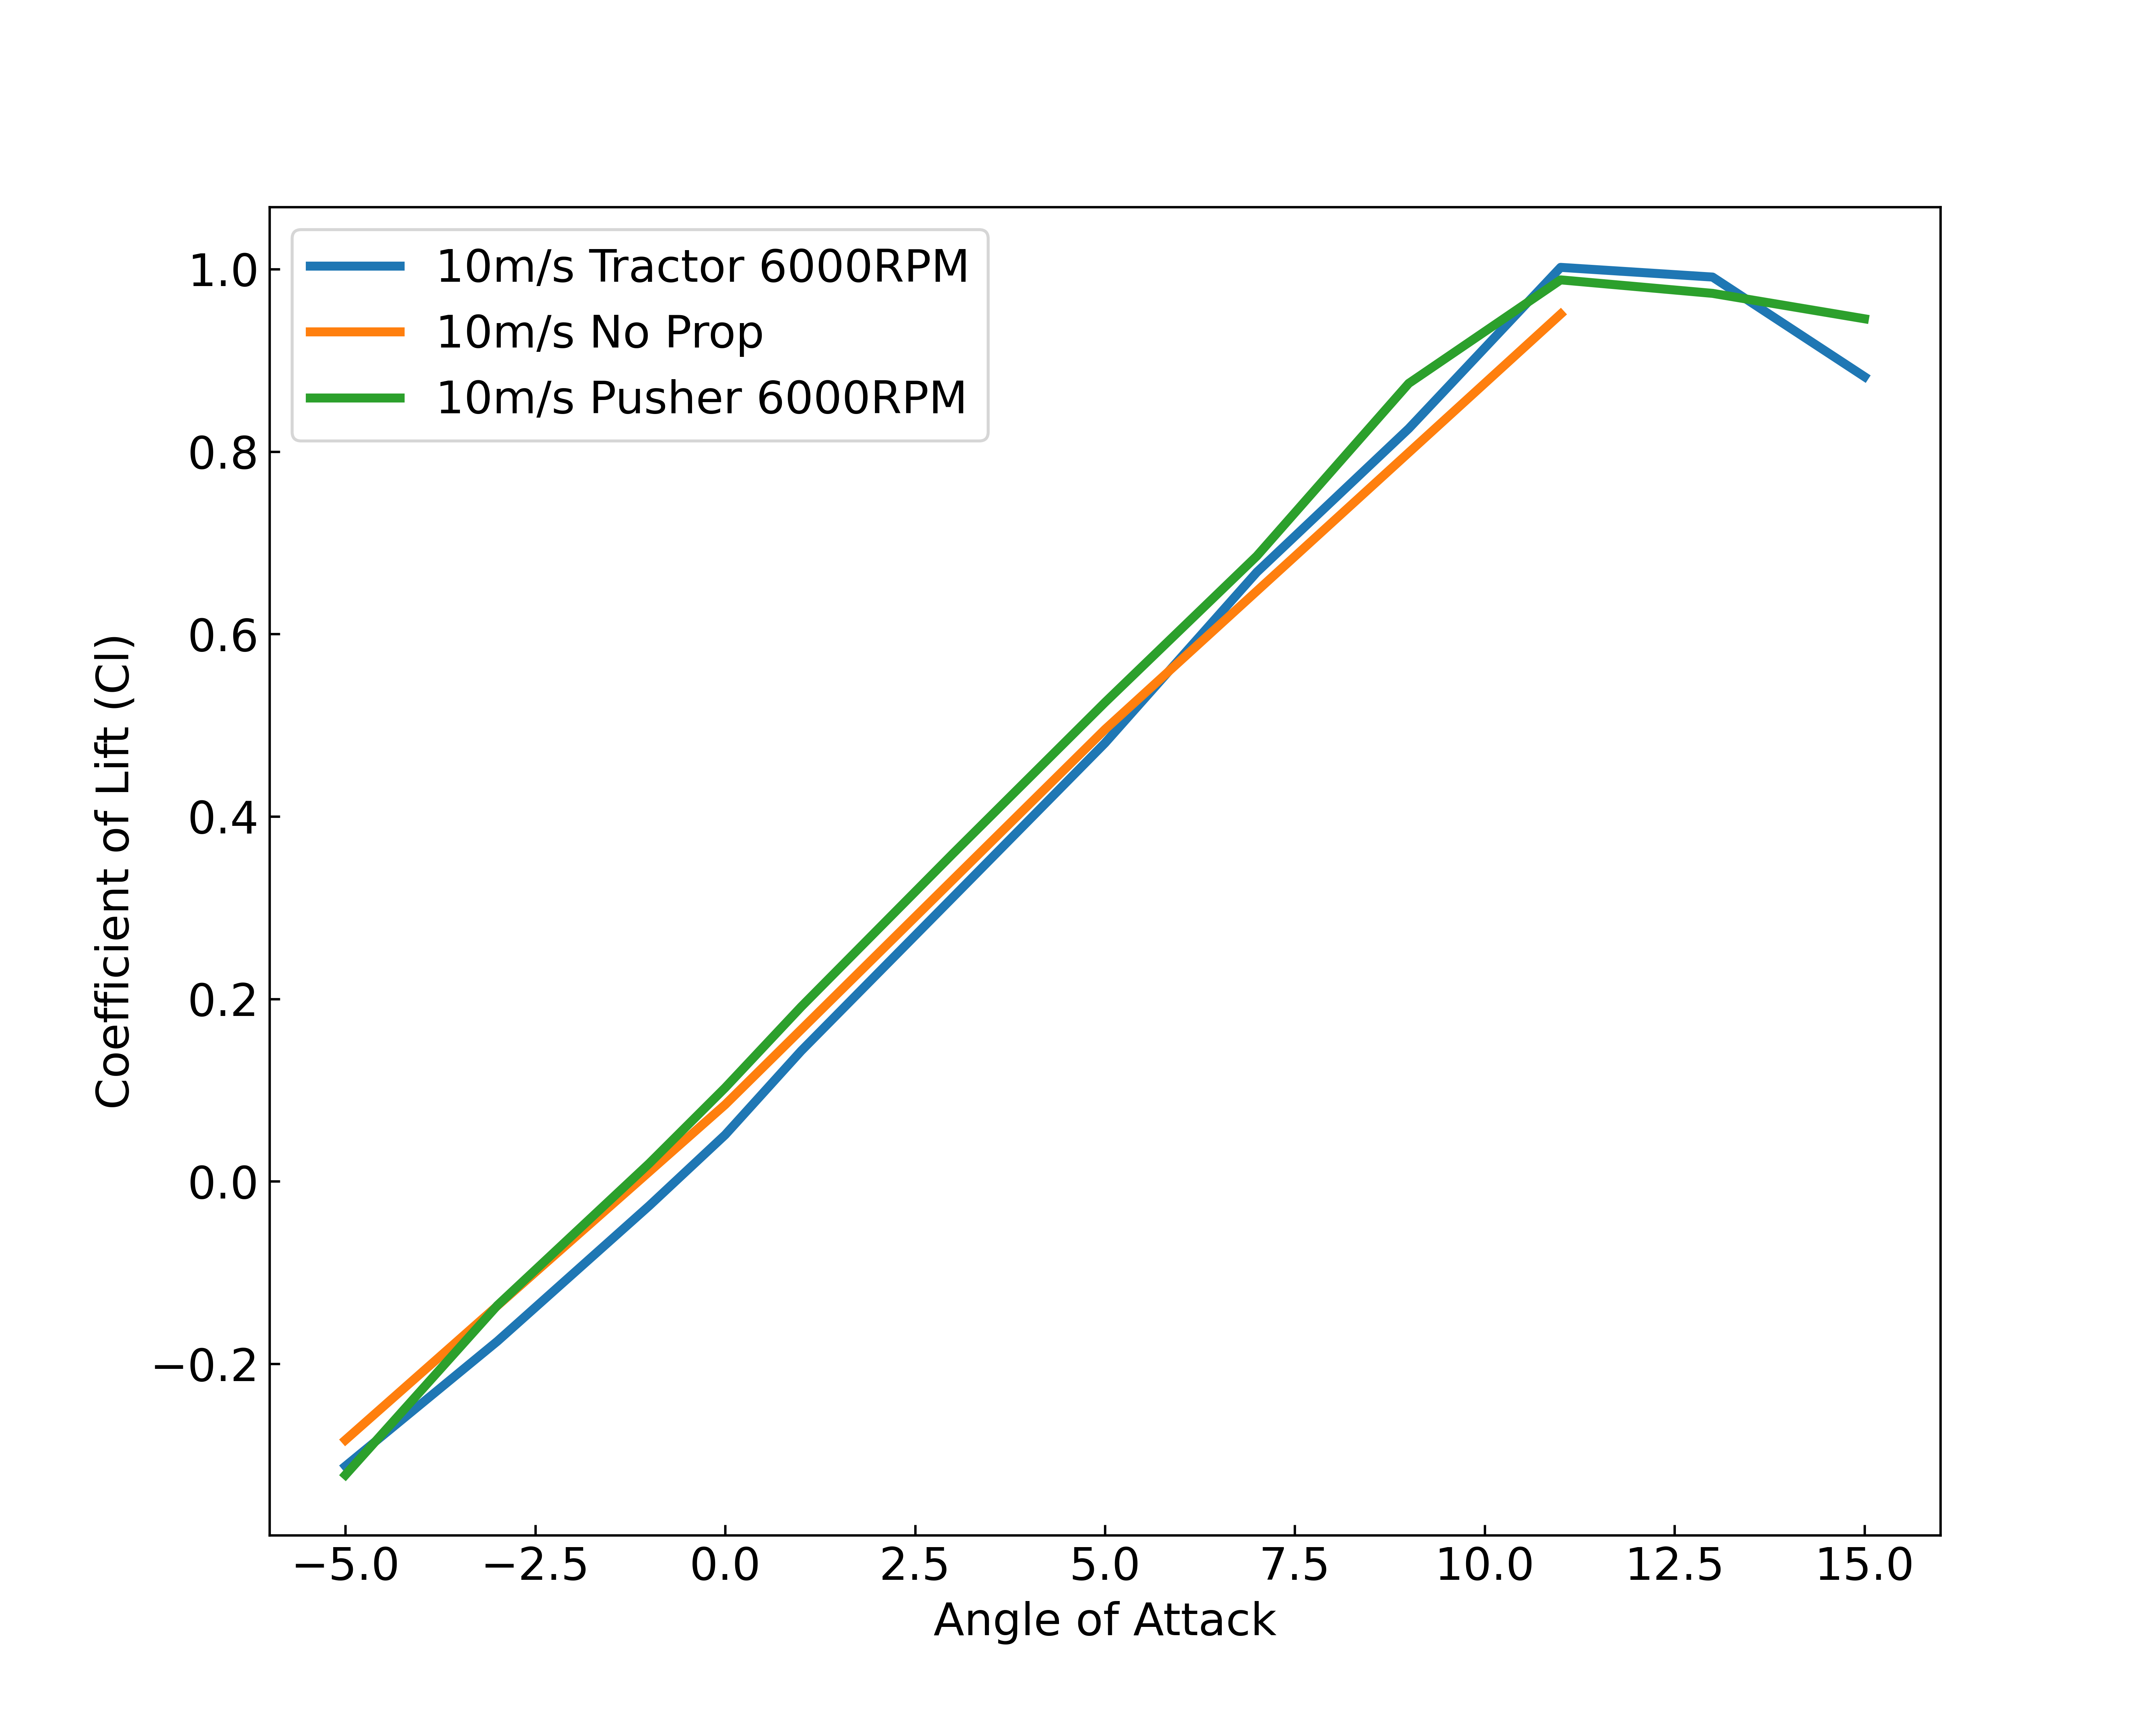
\includegraphics[width=\textwidth]{05_Results/Figs/Cl/10ms_6000RPM_Cl.png}
        \caption{Coefficient of lift at 10m/s airspeed and 6000RPM motor speed}
        \label{fig:Cl_10ms_6000}
    \end{subfigure}
    \begin{subfigure}[b]{0.467\textwidth}
        \centering
        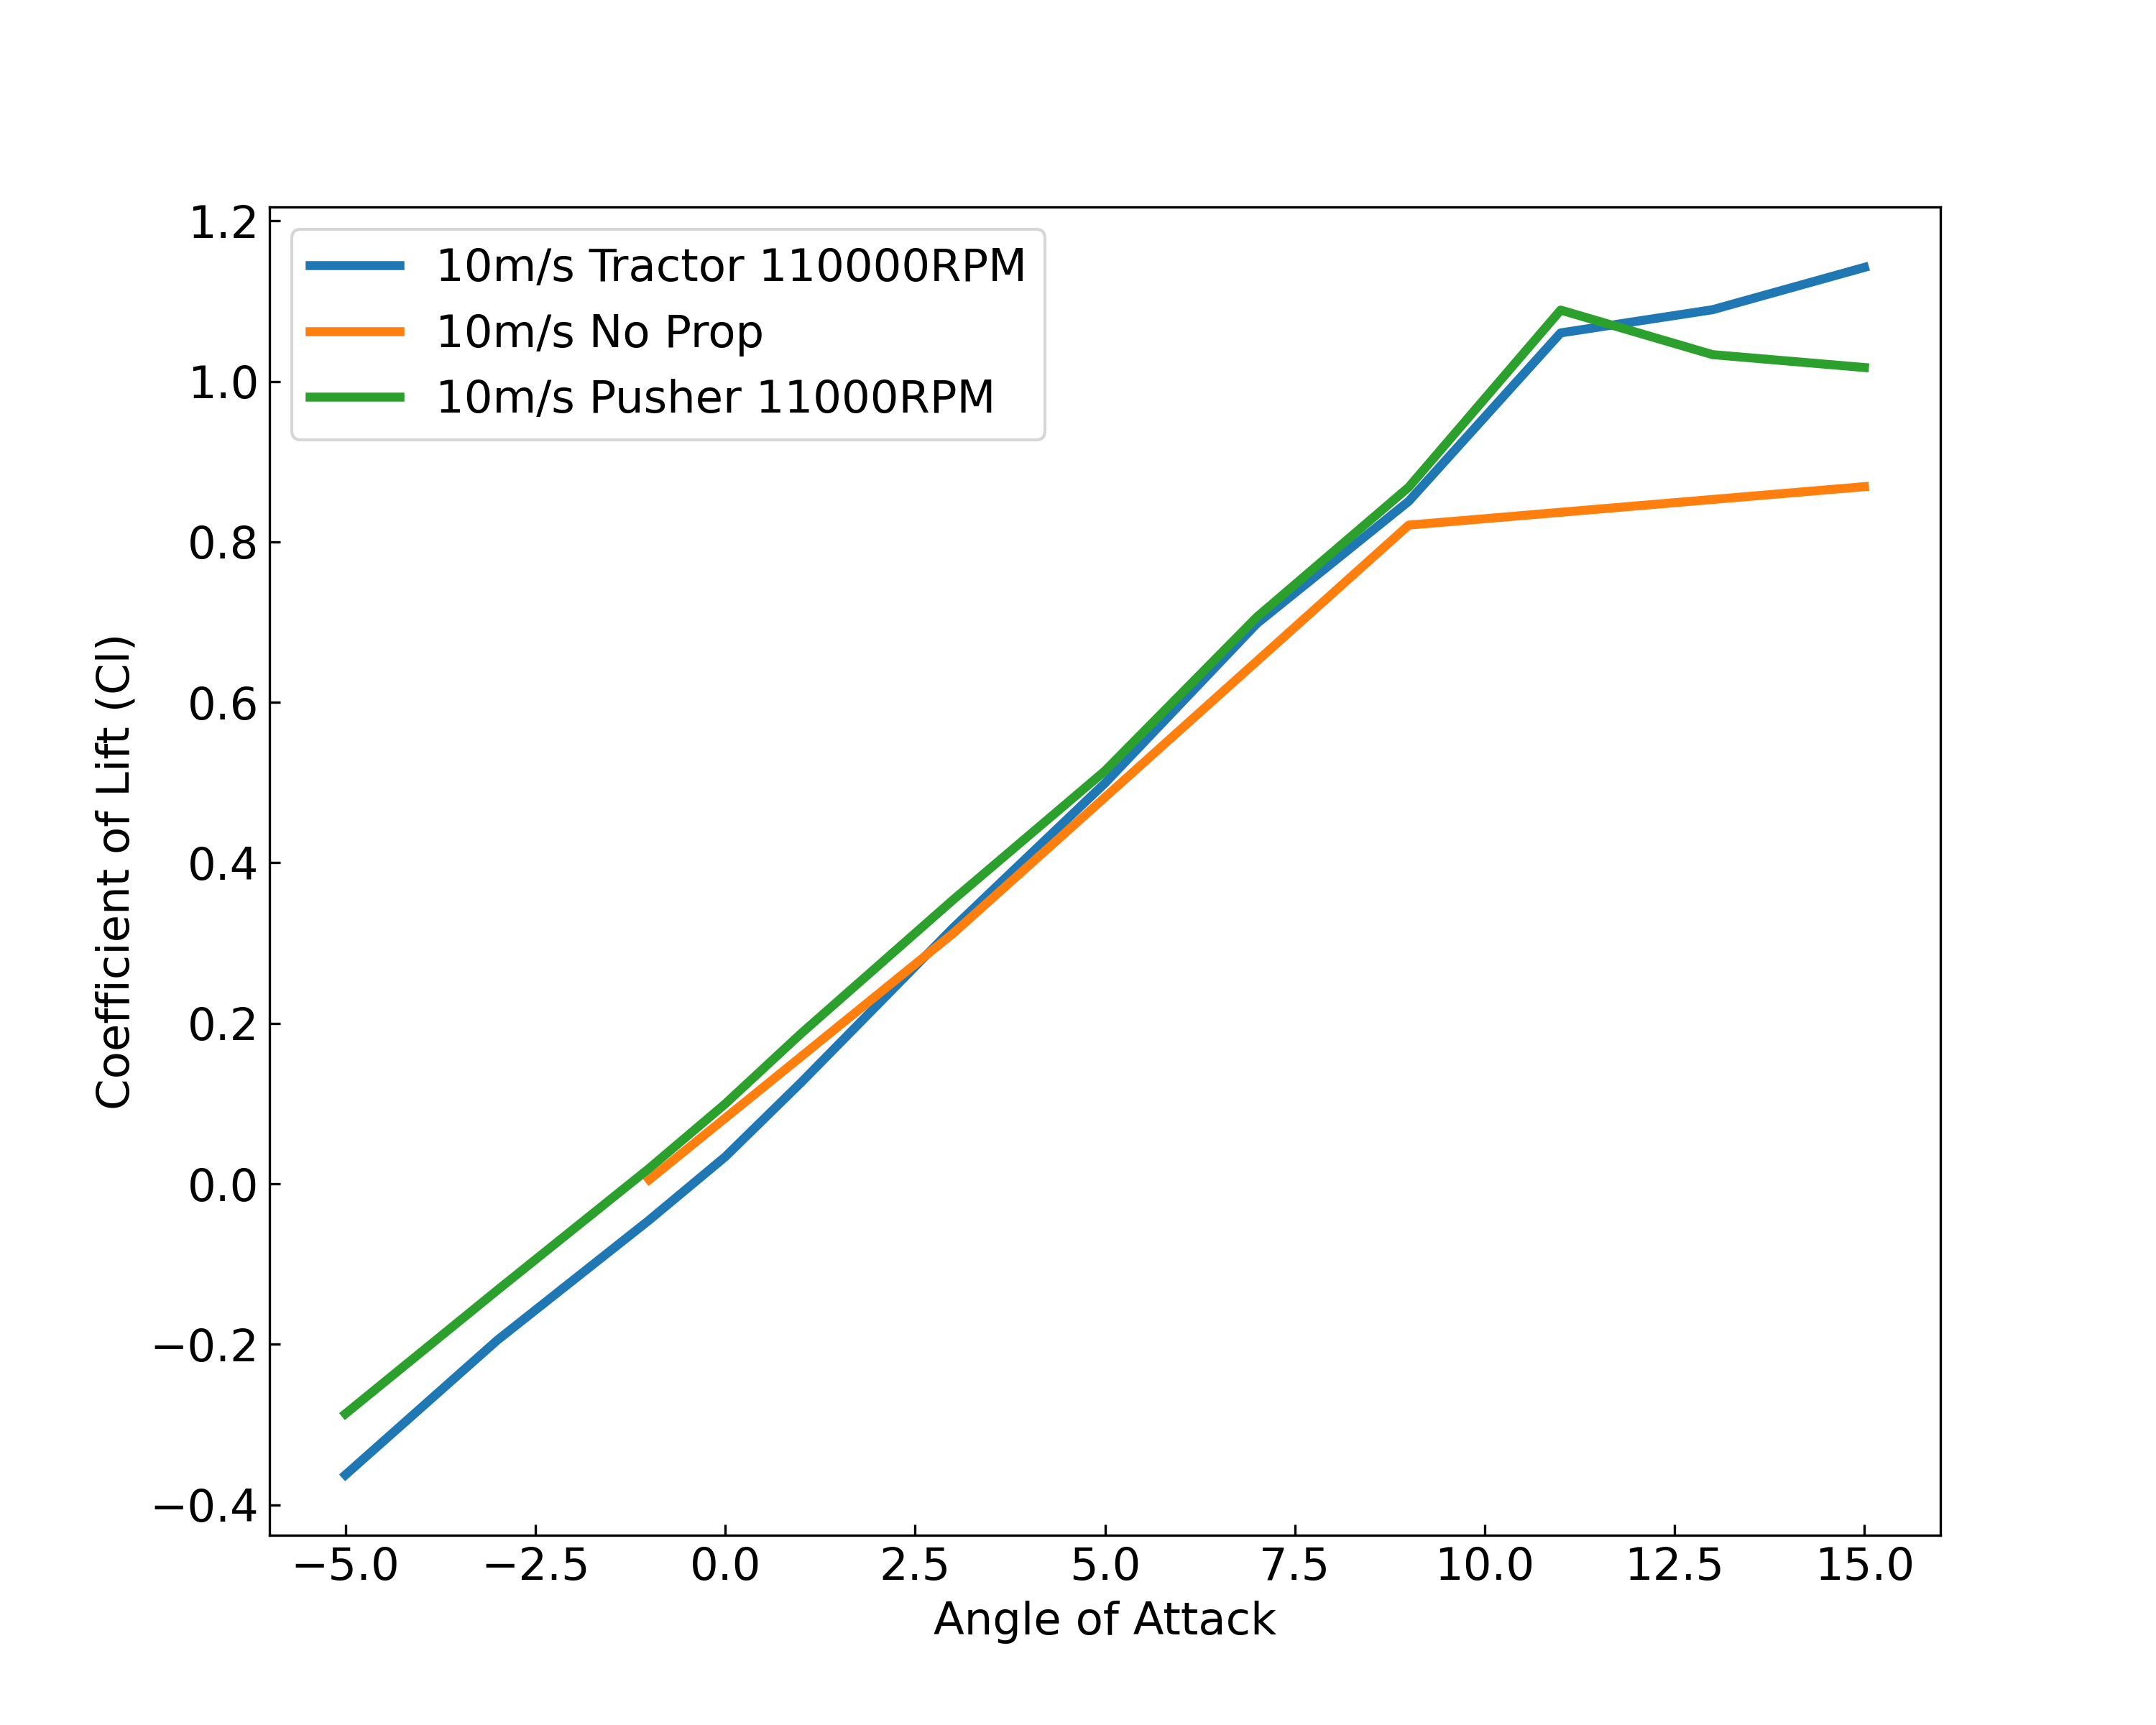
\includegraphics[width=\textwidth]{05_Results/Figs/Cl/10ms_110000RPM_Cl.png}
        \caption{Coefficient of lift at 10m/s airspeed and 11000RPM motor speed}
        \label{fig:Cl_10ms_11000}
    \end{subfigure}
    \begin{subfigure}[b]{0.467\textwidth}
        \centering
        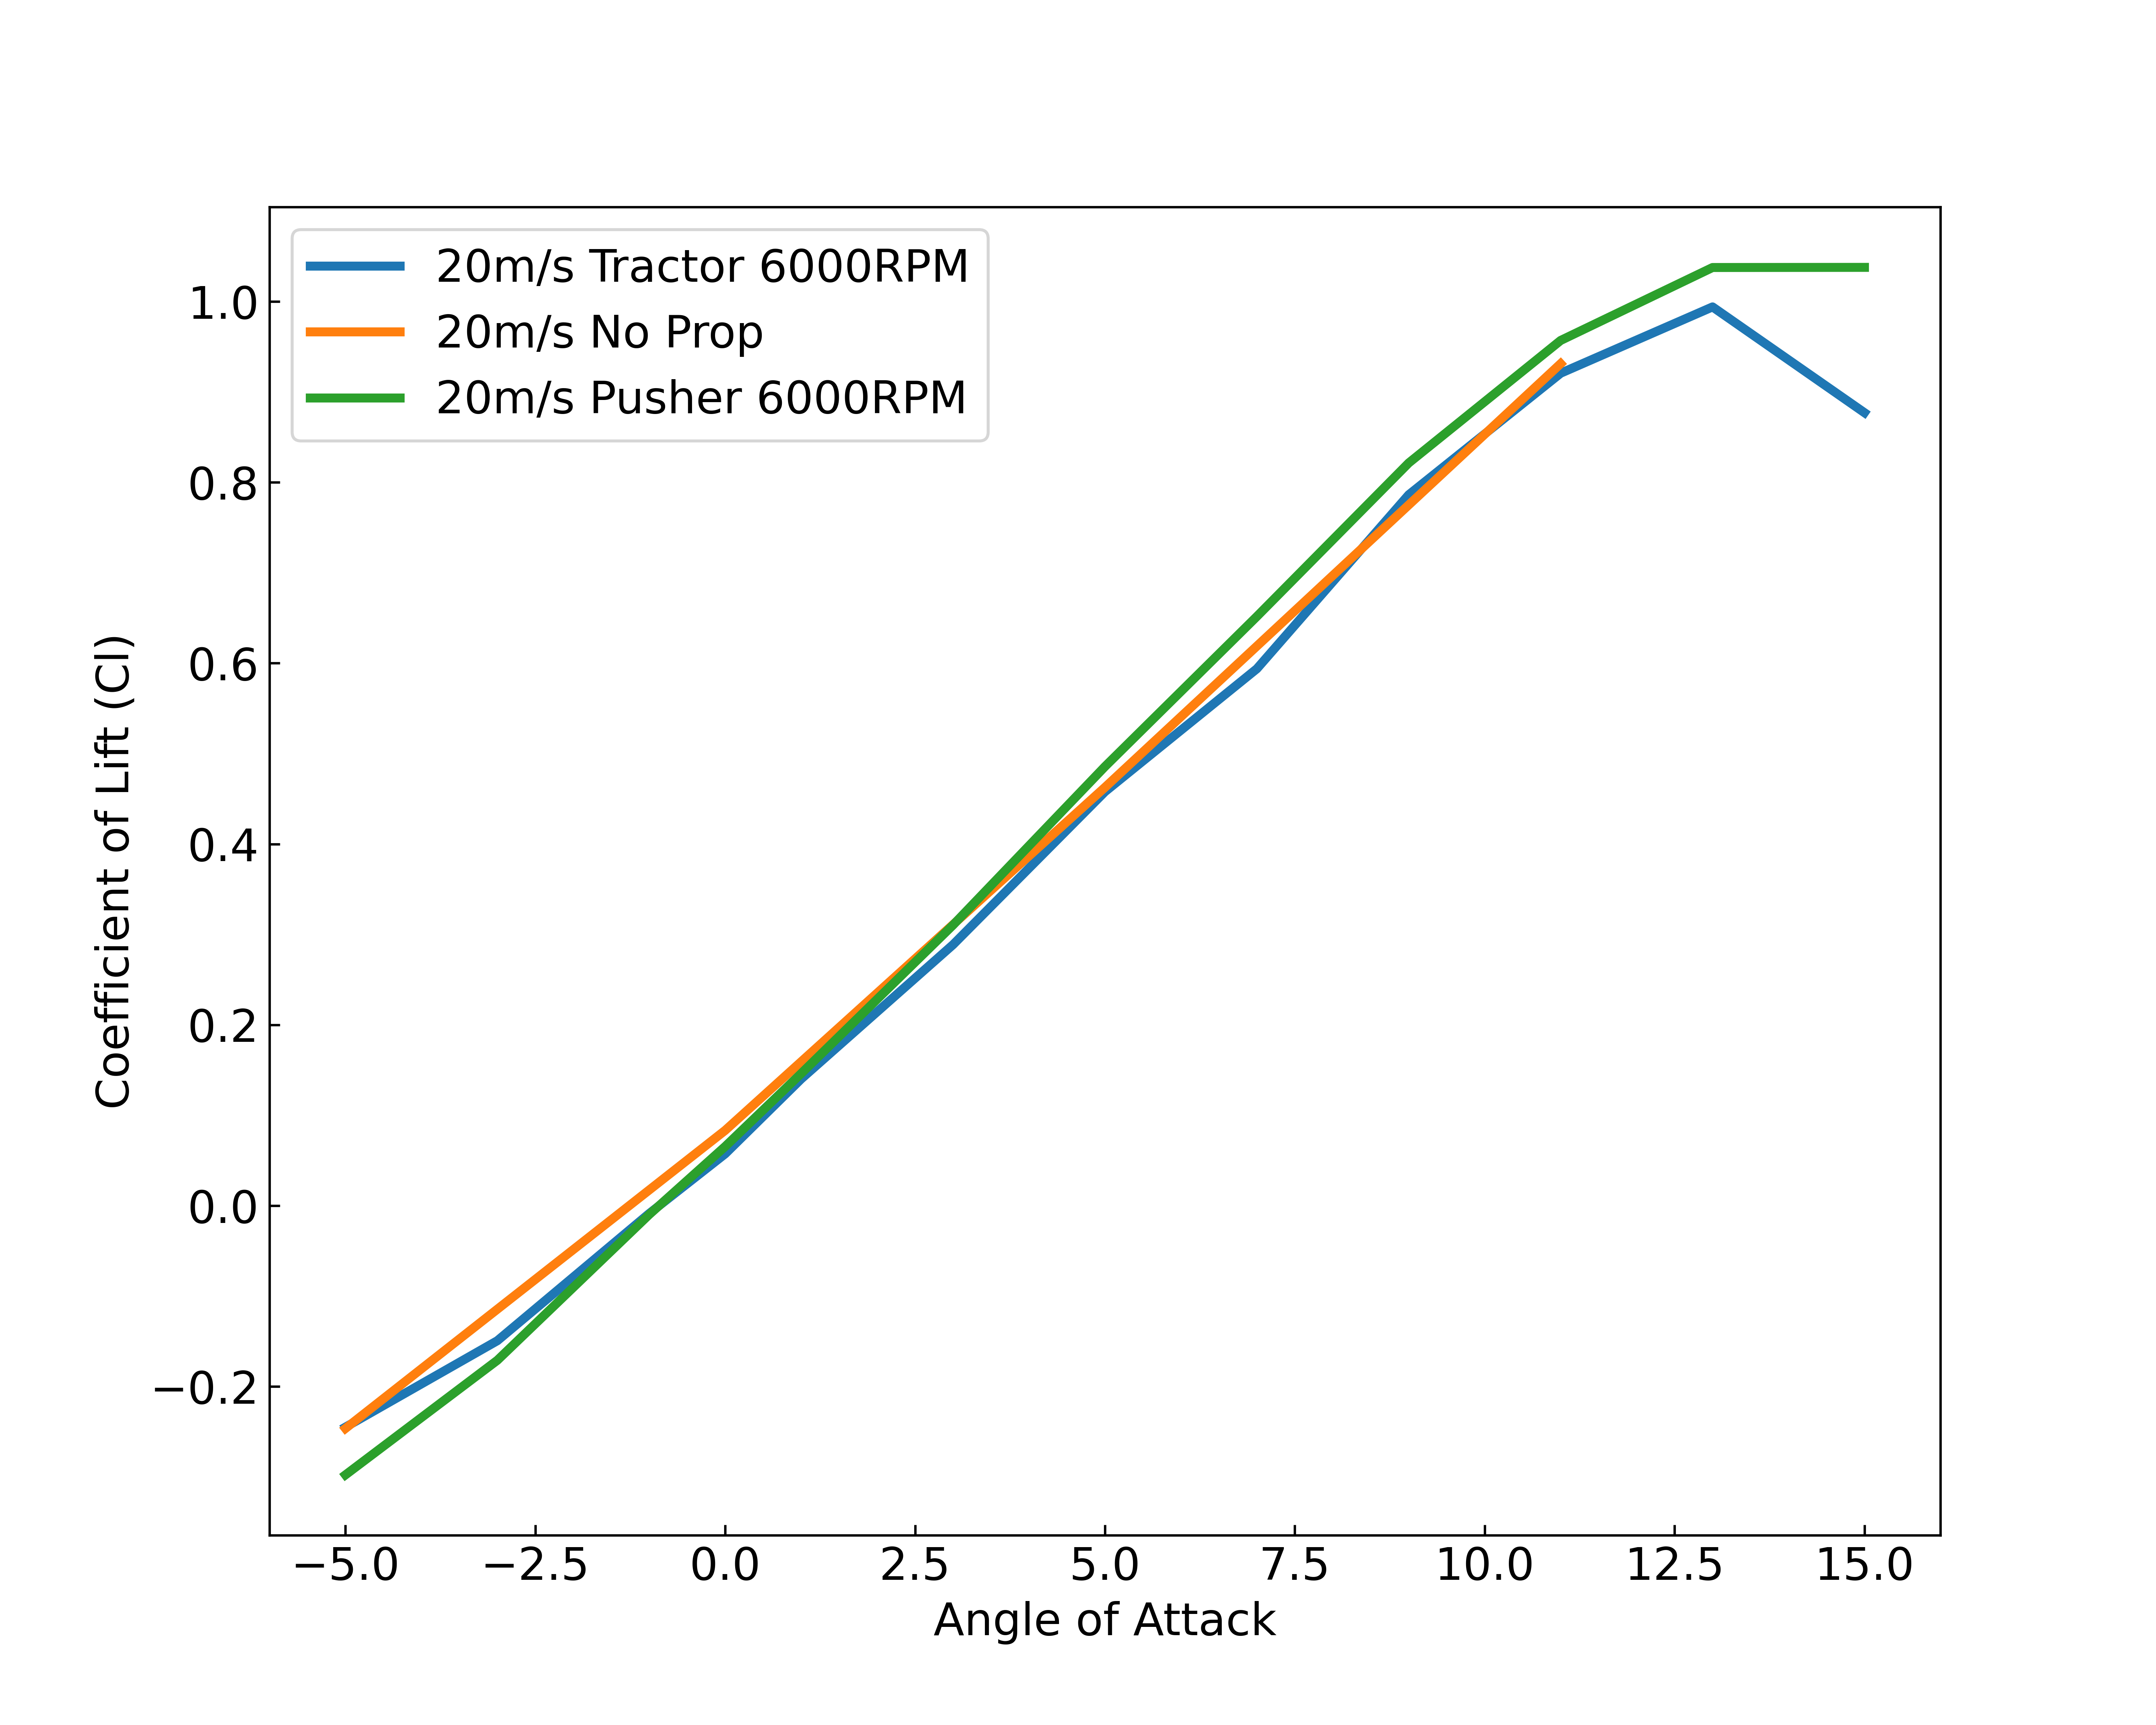
\includegraphics[width=\textwidth]{05_Results/Figs/Cl/20ms_6000RPM_Cl.png}
        \caption{Coefficient of lift at 20m/s airspeed and 6000RPM motor speed}
        \label{fig:Cl_20ms_6000}
    \end{subfigure}
    \begin{subfigure}[b]{0.467\textwidth}
        \centering
        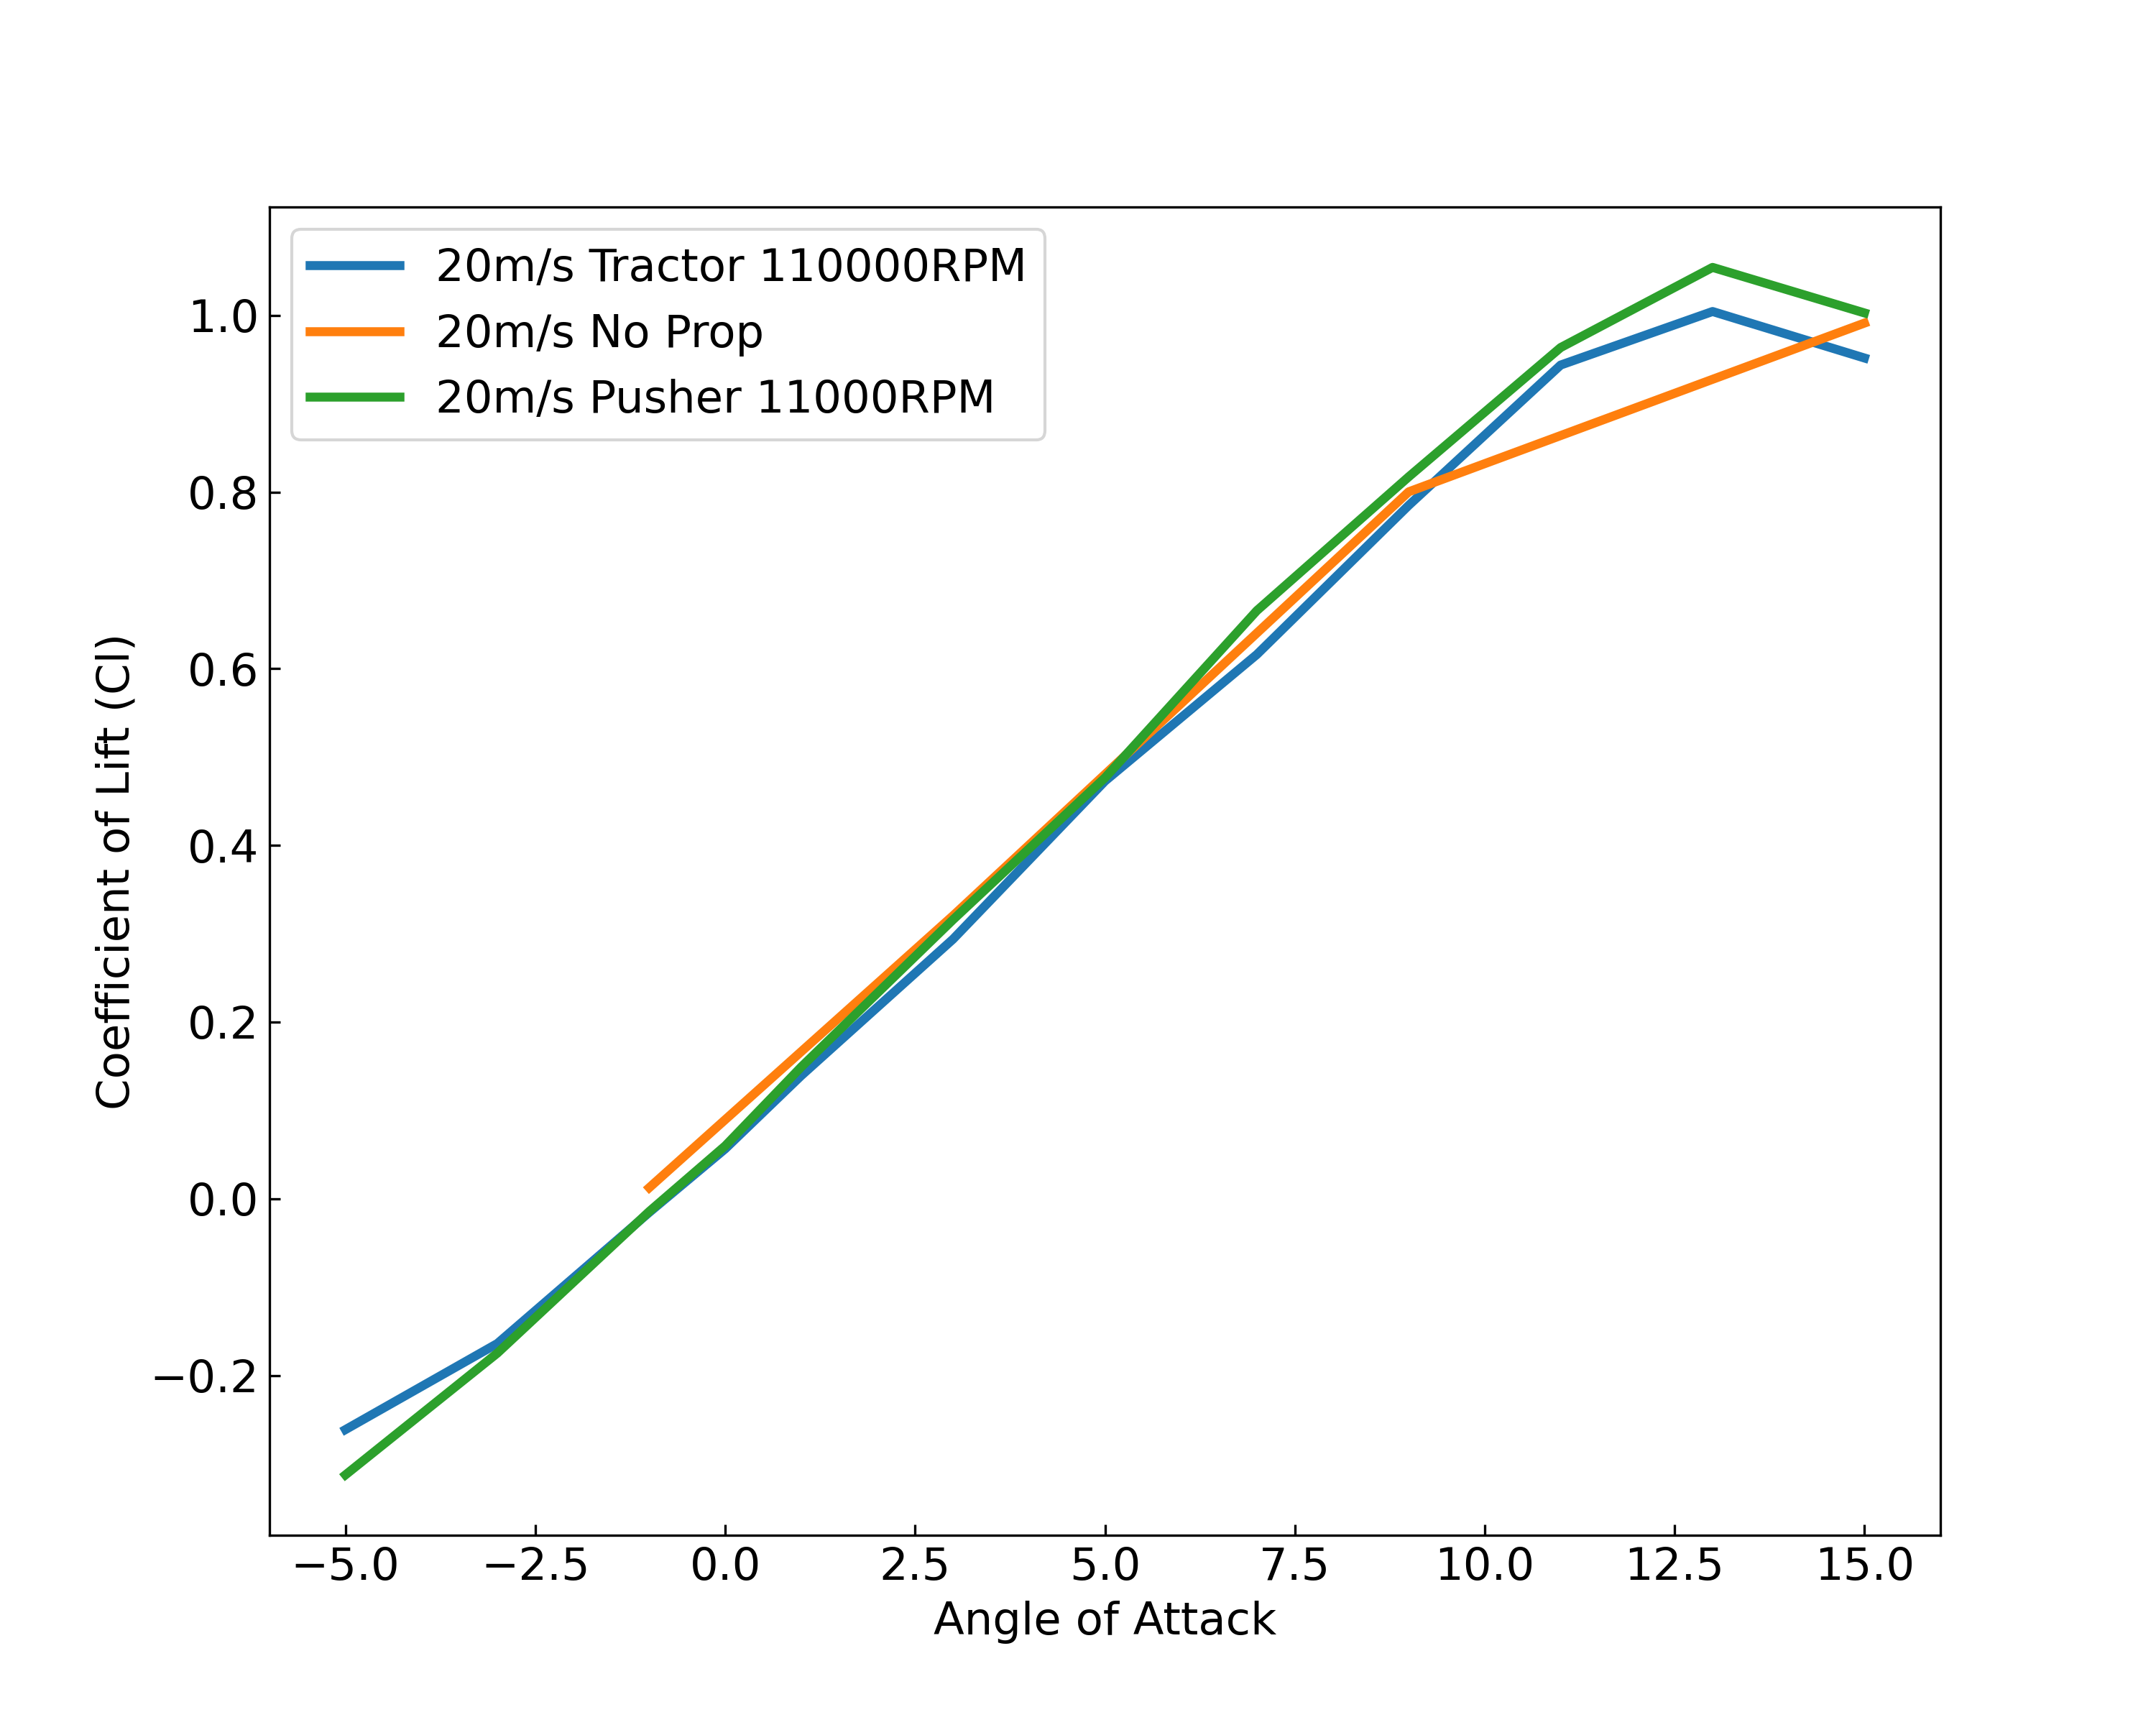
\includegraphics[width=\textwidth]{05_Results/Figs/Cl/20ms_110000RPM_Cl.png}
        \caption{Coefficient of lift at 20m/s airspeed and 11000RPM motor speed}
        \label{fig:Cl_20ms_11000}
    \end{subfigure}
    \caption{Coefficient of lift variation with various conditions for the pusher, tractor and no propeller configurations }
\end{figure}

\subsection{Aerodynamic Coefficient of Thrust Minus Drag Force}
Figure \ref{fig:Cd_11000RPM} shows that as the wind tunnel airspeed increased, the thrust minus drag coefficient (referred to as the force coefficient) shifted upwards for both the pusher and tractor configuration. The overall force for both the tractor and puller configuration at 10m$s^{-1}$ airspeed is negative and shifts to positive value as the airspeed increases to 20m$s^{-1}$. This is due to the thrust produced by the propeller decreasing as the airspeed increases for both the tractor and puller configurations. The force curve shifts into negative values for the tractor and puller configurations due to the thrust produced by the propeller. As the overall force is a measure of the thrust minus drag, the overall force becomes negative, shifting the coefficient of force curve into negative values. As the airspeed increases, the force coefficient is also seen to increase for the pusher and tractor configuration with increasing airspeed. This shifts the coefficient of force curves upwards as the airspeed increases. The highest force coefficient occurred when no propeller operated on the \acrshort{MAV} model. Ananda concluded that for tractor configuration propeller-wing set up in a low-speed wind tunnel, the flow transitions to turbulent flow earlier. This reduces the drag and increases the lift-to-drag ratio \cite{Ananda2018}. This shows a discrepancy with the results seen in this study. However, Ananda's setup involved a motor being mounted in front of the wing with no direct attachment; hence, the forces are not directly applied to the wing \cite{Ananda2018}. When no propeller is added, no significant changes are seen in airspeed for the force coefficient. The tractor configuration, in general, has a lower overall thrust minus drag than the pusher configuration; hence, the force coefficient is lower for the tractor configuration. This is most clearly seen at 20m$s^{-1}$ in Figure \ref{fig:Cd_11000RPM}. This could possibly be due to less thrust being produced in the tractor configuration, however further investigation is needed as the motor thrust was not separately measured during wind tunnel testing. 




\begin{figure}[H]
    \centering
    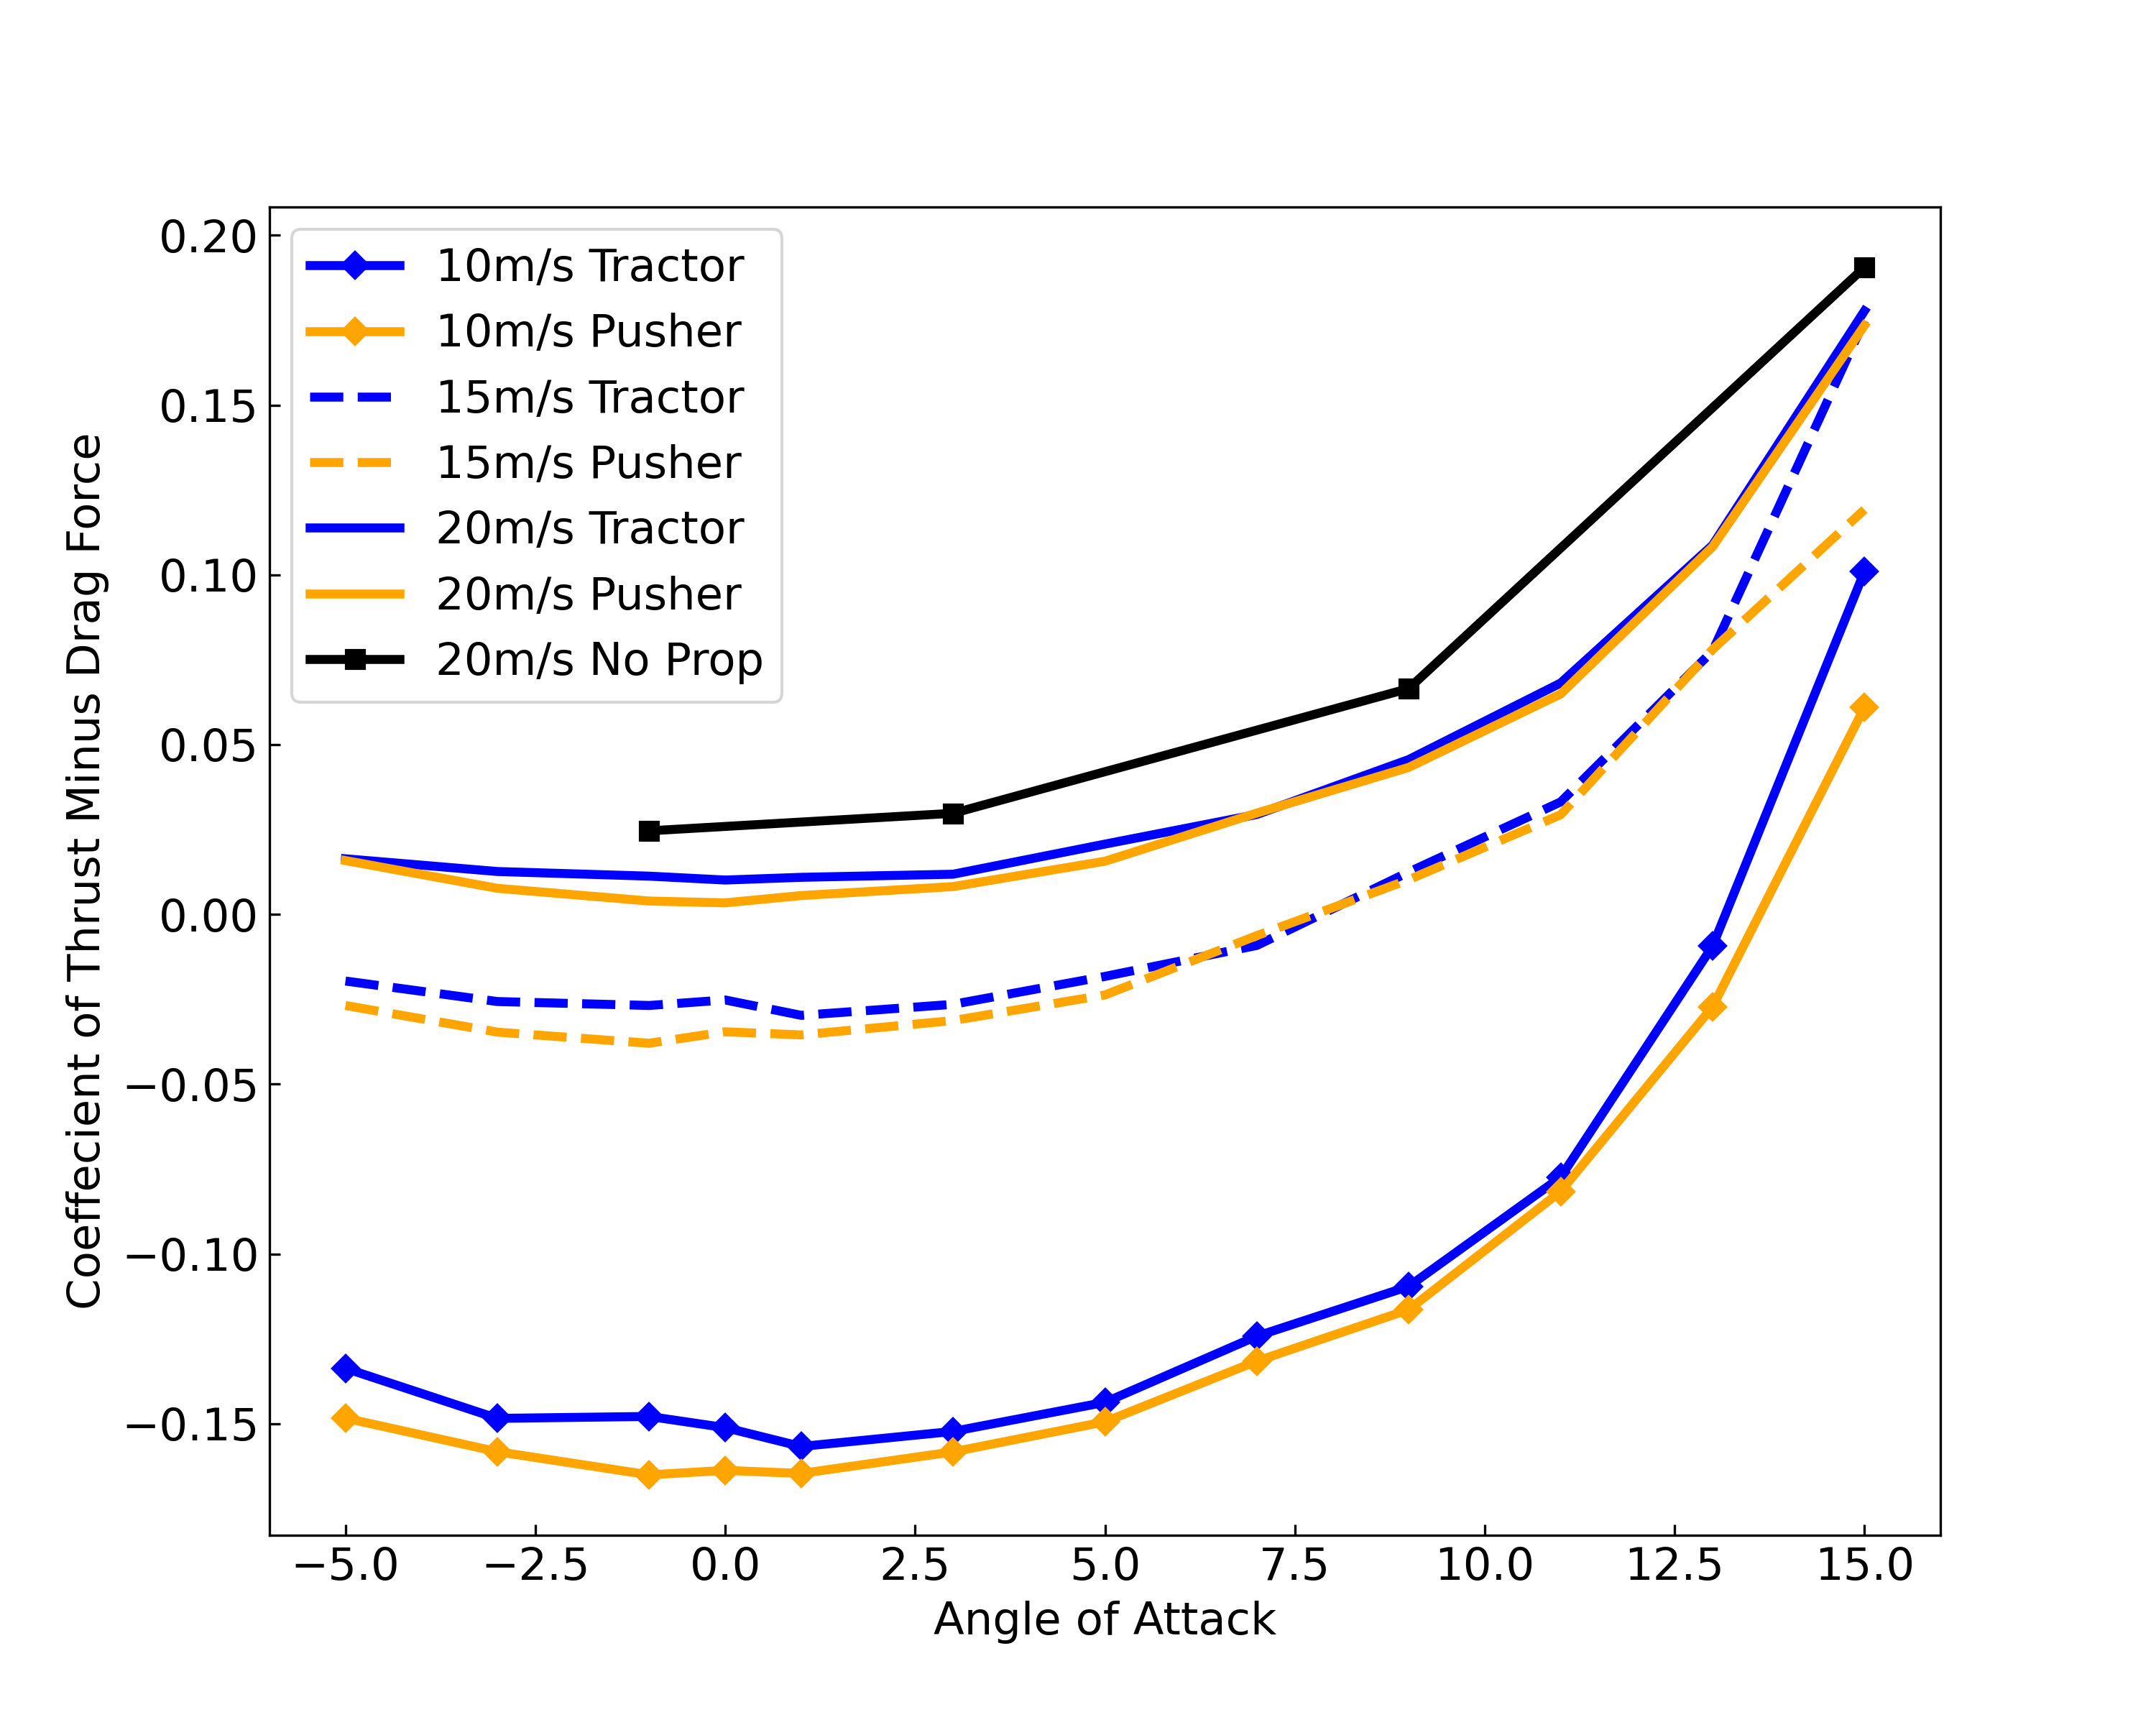
\includegraphics[scale = 0.45]{05_Results/Figs/Cd/110000RPM_Cd.png}
    \caption{Coefficient of drag variation at 11000RPM motor speed for the tractor, pusher and no propeller configurations}
    \label{fig:Cd_11000RPM}
\end{figure}

Figure \ref{fig:tesing2} shows that the coefficient of force shifts downwards as the propeller RPM increases from 6000RPM to 11000RPM at an airspeed of 10m$s^{-1}$. This trend changes as the airspeed increases due to the propellers beginning to windmill as the airspeed increases to 20m$s^{-1}$ (the tractor and pusher configuration at 6000RPM propeller as shown in Appendix \ref{app:wtr}). The increased propeller adds additional drag to the \acrshort{MAV} model causing this shift in the coefficient of force downwards. The tractor configuration again has a lower overall thrust minus drag than the pusher configuration, conclusive reasons for this cannot be made as the motor thrust was not separately recorded. 


\begin{figure}[H]
    \centering
    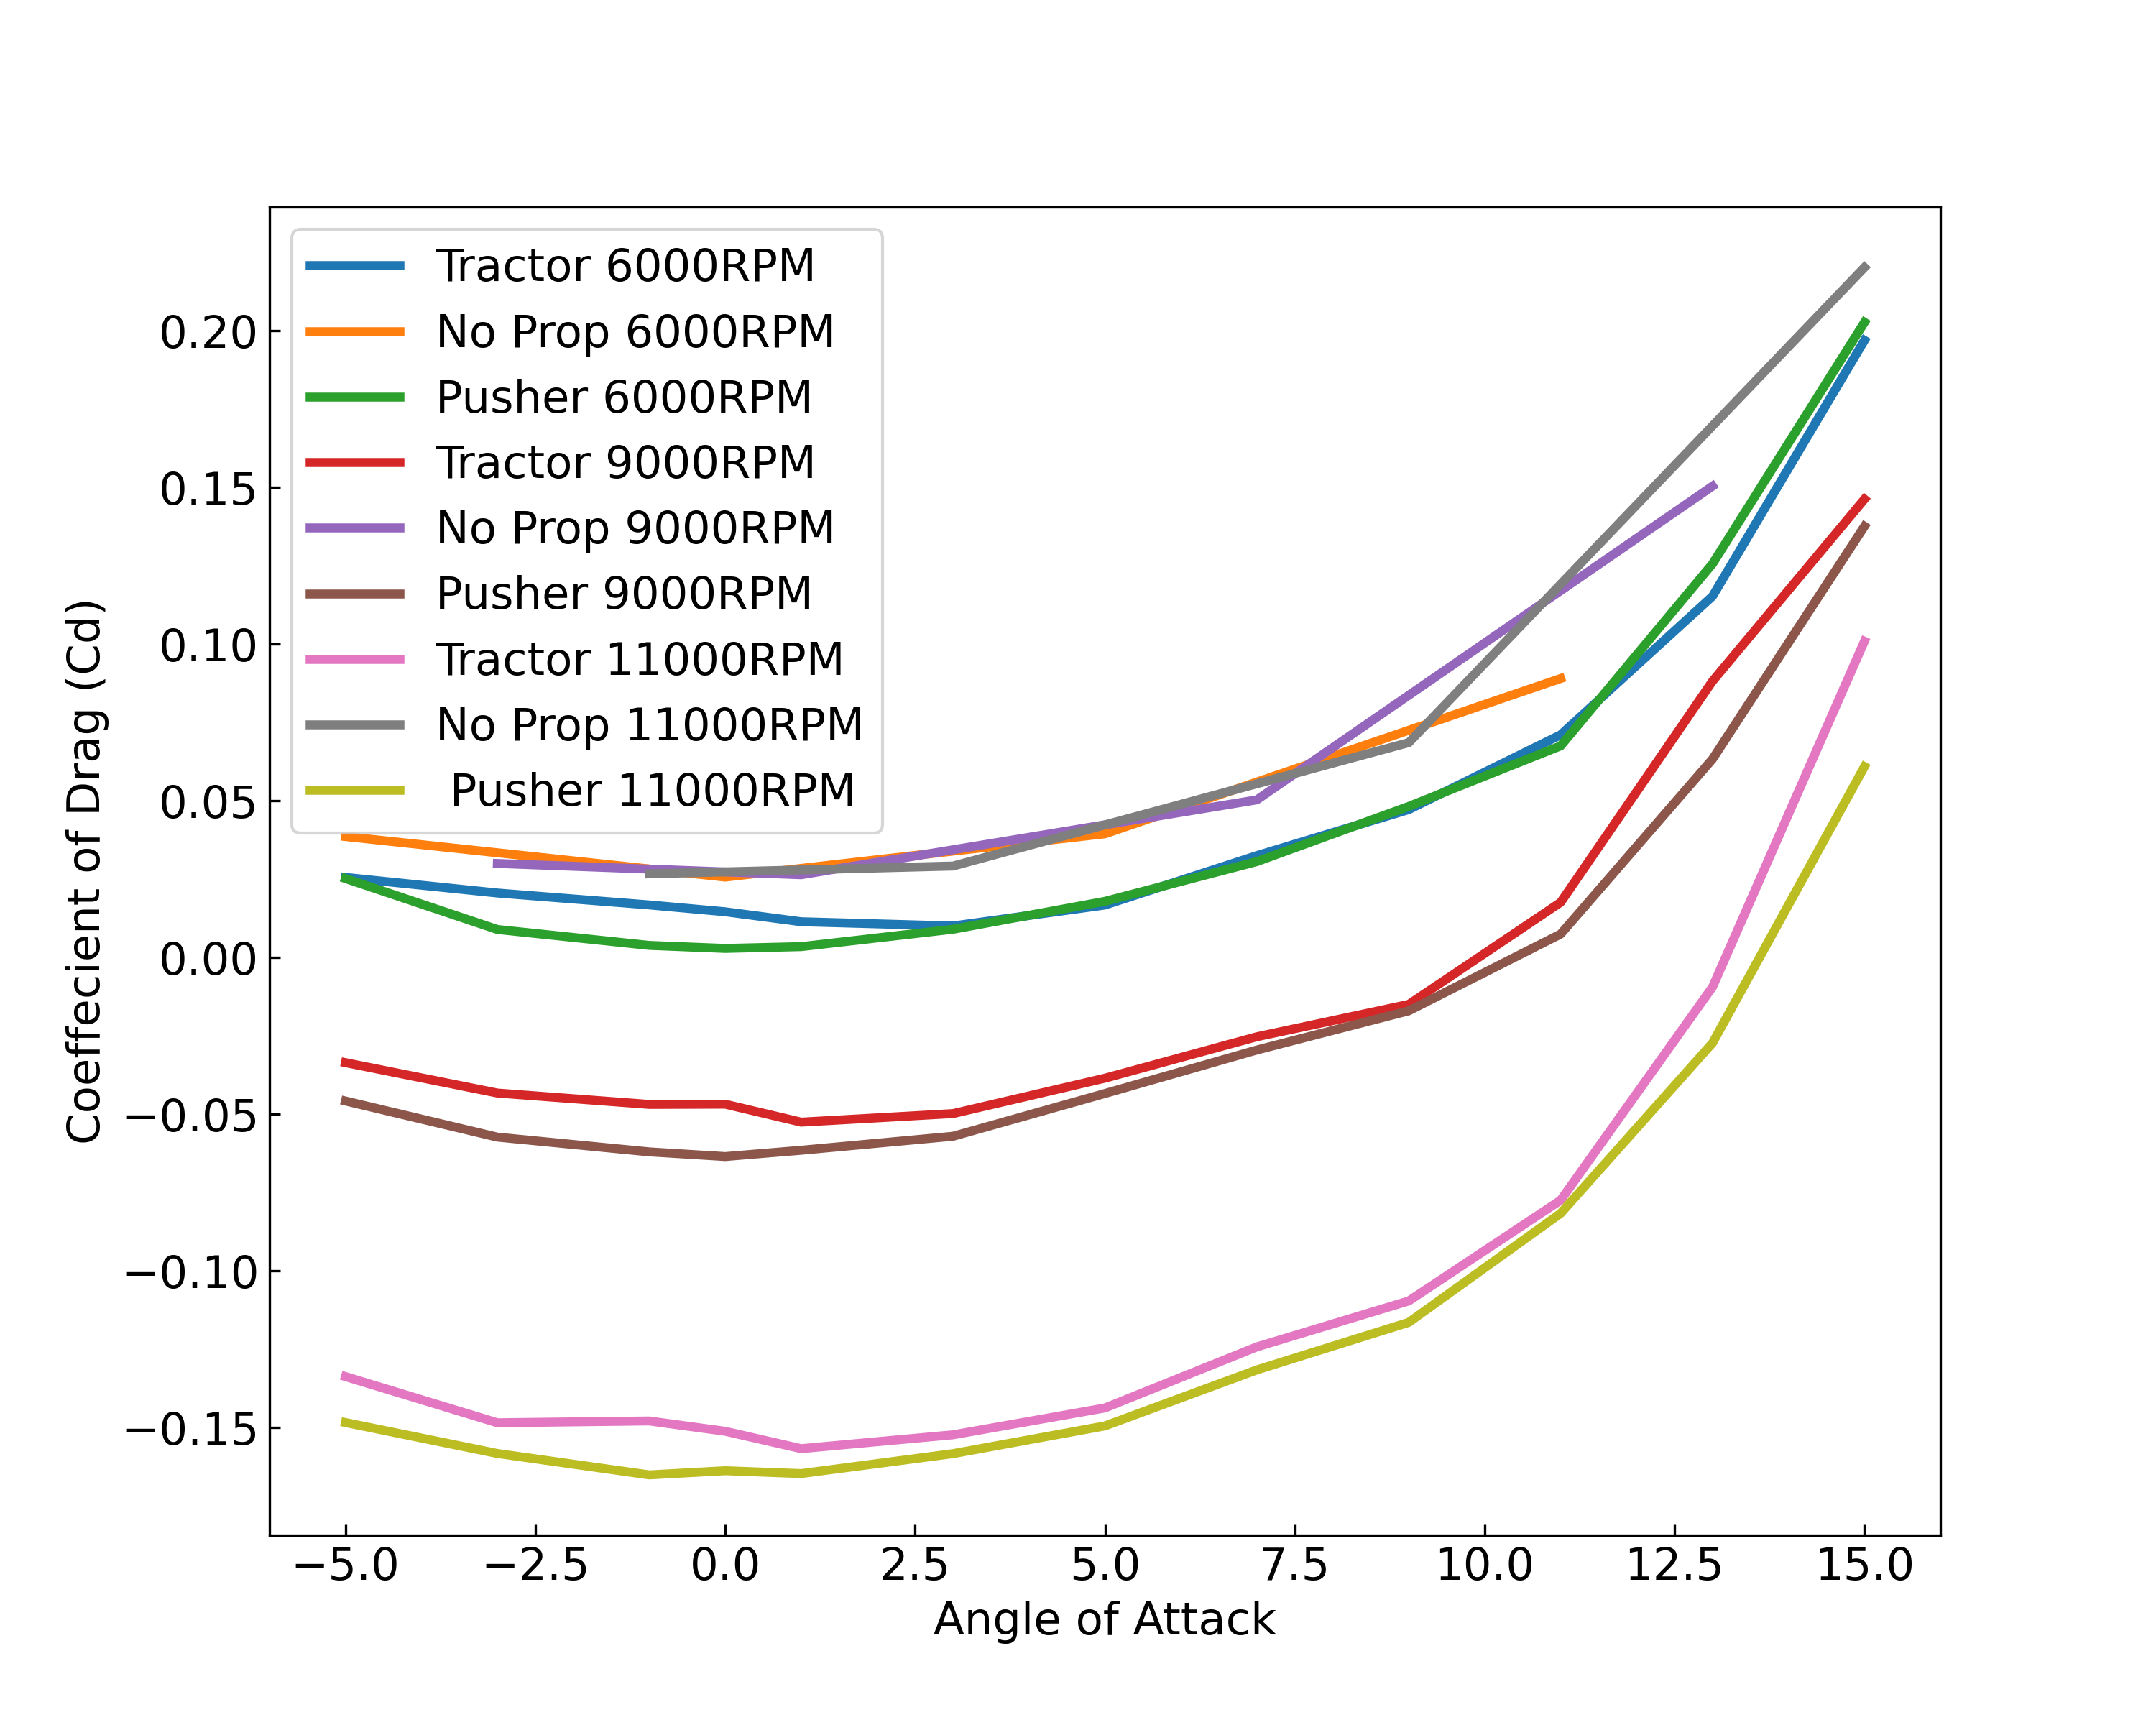
\includegraphics[scale = 0.45]{05_Results/Figs/Cd/10ms_Cd.png}
    \caption{Coefficient of drag variation at 10ms airspeed for the tractor, pusher and no propeller configuration}
    \label{fig:tesing2}
\end{figure}



\subsection{Pitching Moment Coefficient}

Figures \ref{fig:Cm_10ms_6000} to \ref{fig:Cm_20ms_11000} show that for all cases, the pitching moment of the \acrshort{MAV} model decreases as the angle of attack increases. This leads to a stable \acrshort{MAV} in all cases as the longitudinal stability is maintained due to the pitching down motion of the \acrshort{MAV} as the \acrshort{AoA} increases. Figures \ref{fig:Cm_10ms_6000} to \ref{fig:Cm_20ms_11000} also show that as the motor speed increases from 6000RPM to 11000RPM, the tractor configuration experienced a decrease in pitching coefficient compared with the no propeller model up until stall at approximately 12$^\circ$ \acrshort{AoA}. The pusher configuration experienced an increase in the pitching moment compared with the no-propeller model. This shows that as the airspeed and propeller speed increase, the tractor configuration becomes less stable, while the pusher configuration becomes more stable. Increasing the airspeed decreased the pitching moment for all motor speeds.

\begin{figure}[H]
    \centering
    \begin{subfigure}[b]{0.467\textwidth}
        \centering
        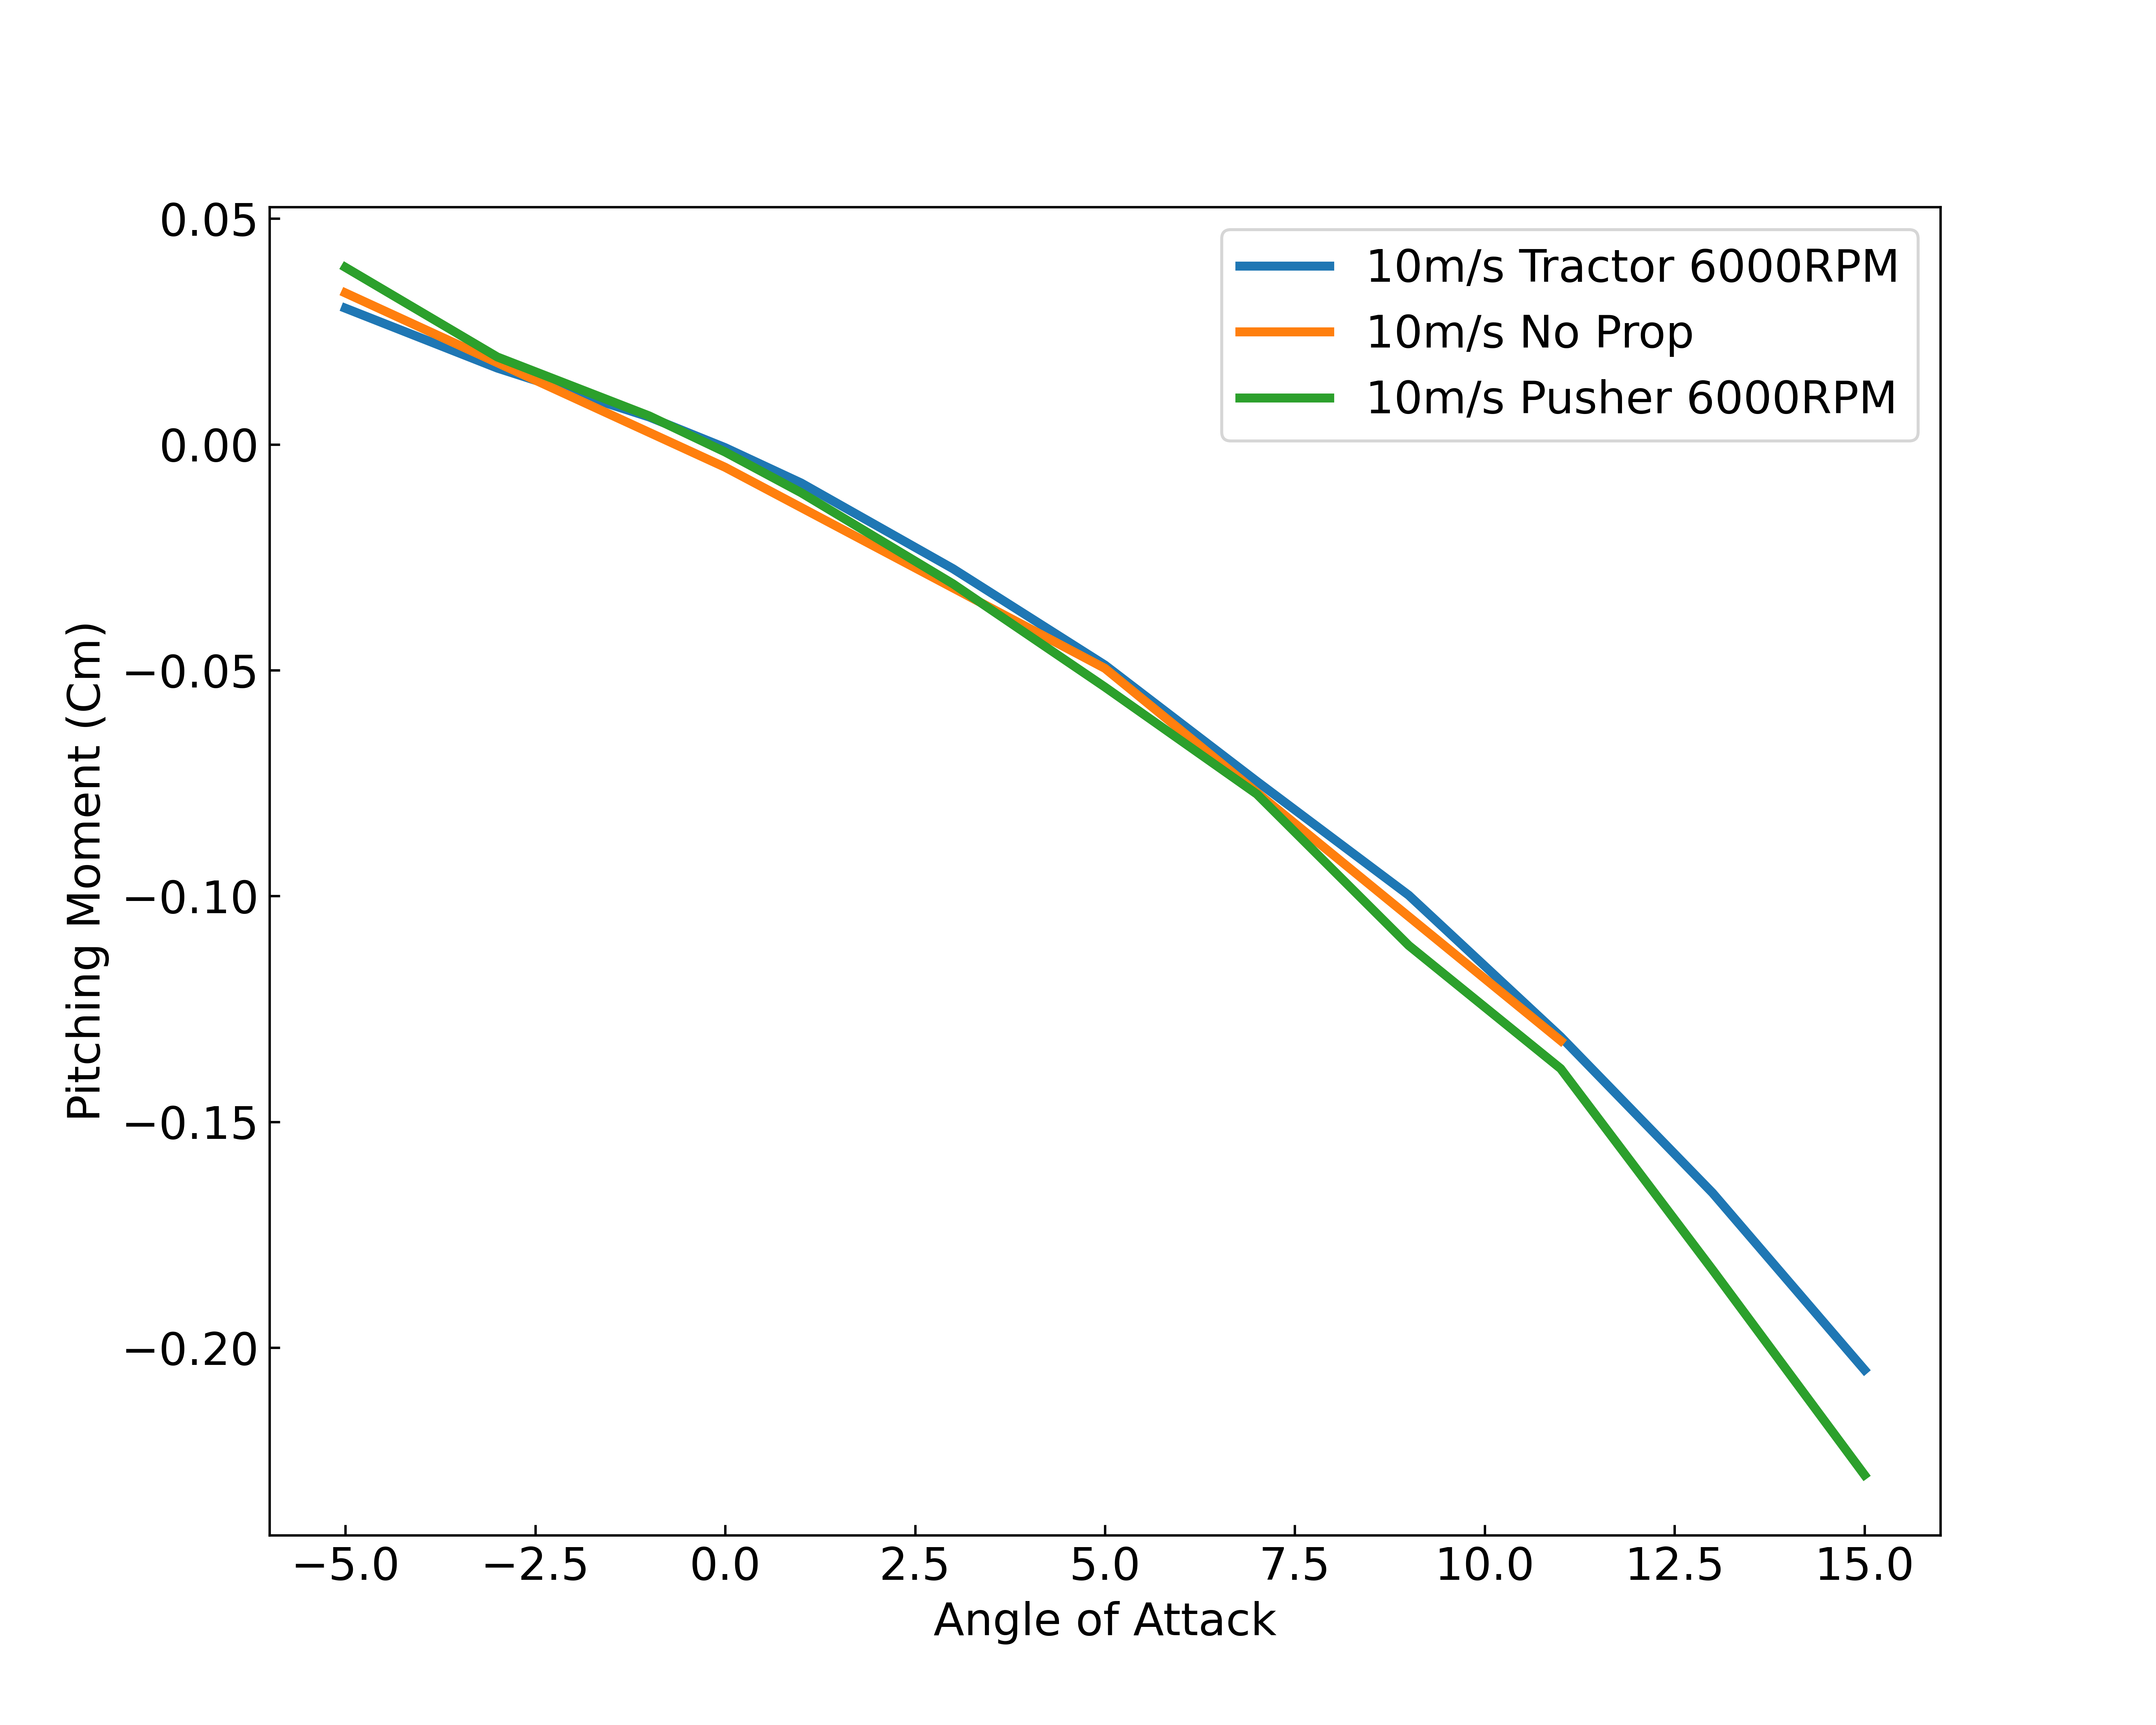
\includegraphics[width=\textwidth]{05_Results/Figs/Cm/10ms_6000RPM_Cm.png}
        \caption{Pitching Moment Coefficient at 10m/s airspeed and 6000RPM motor speed}
        \label{fig:Cm_10ms_6000}
    \end{subfigure}
    \begin{subfigure}[b]{0.467\textwidth}
        \centering
        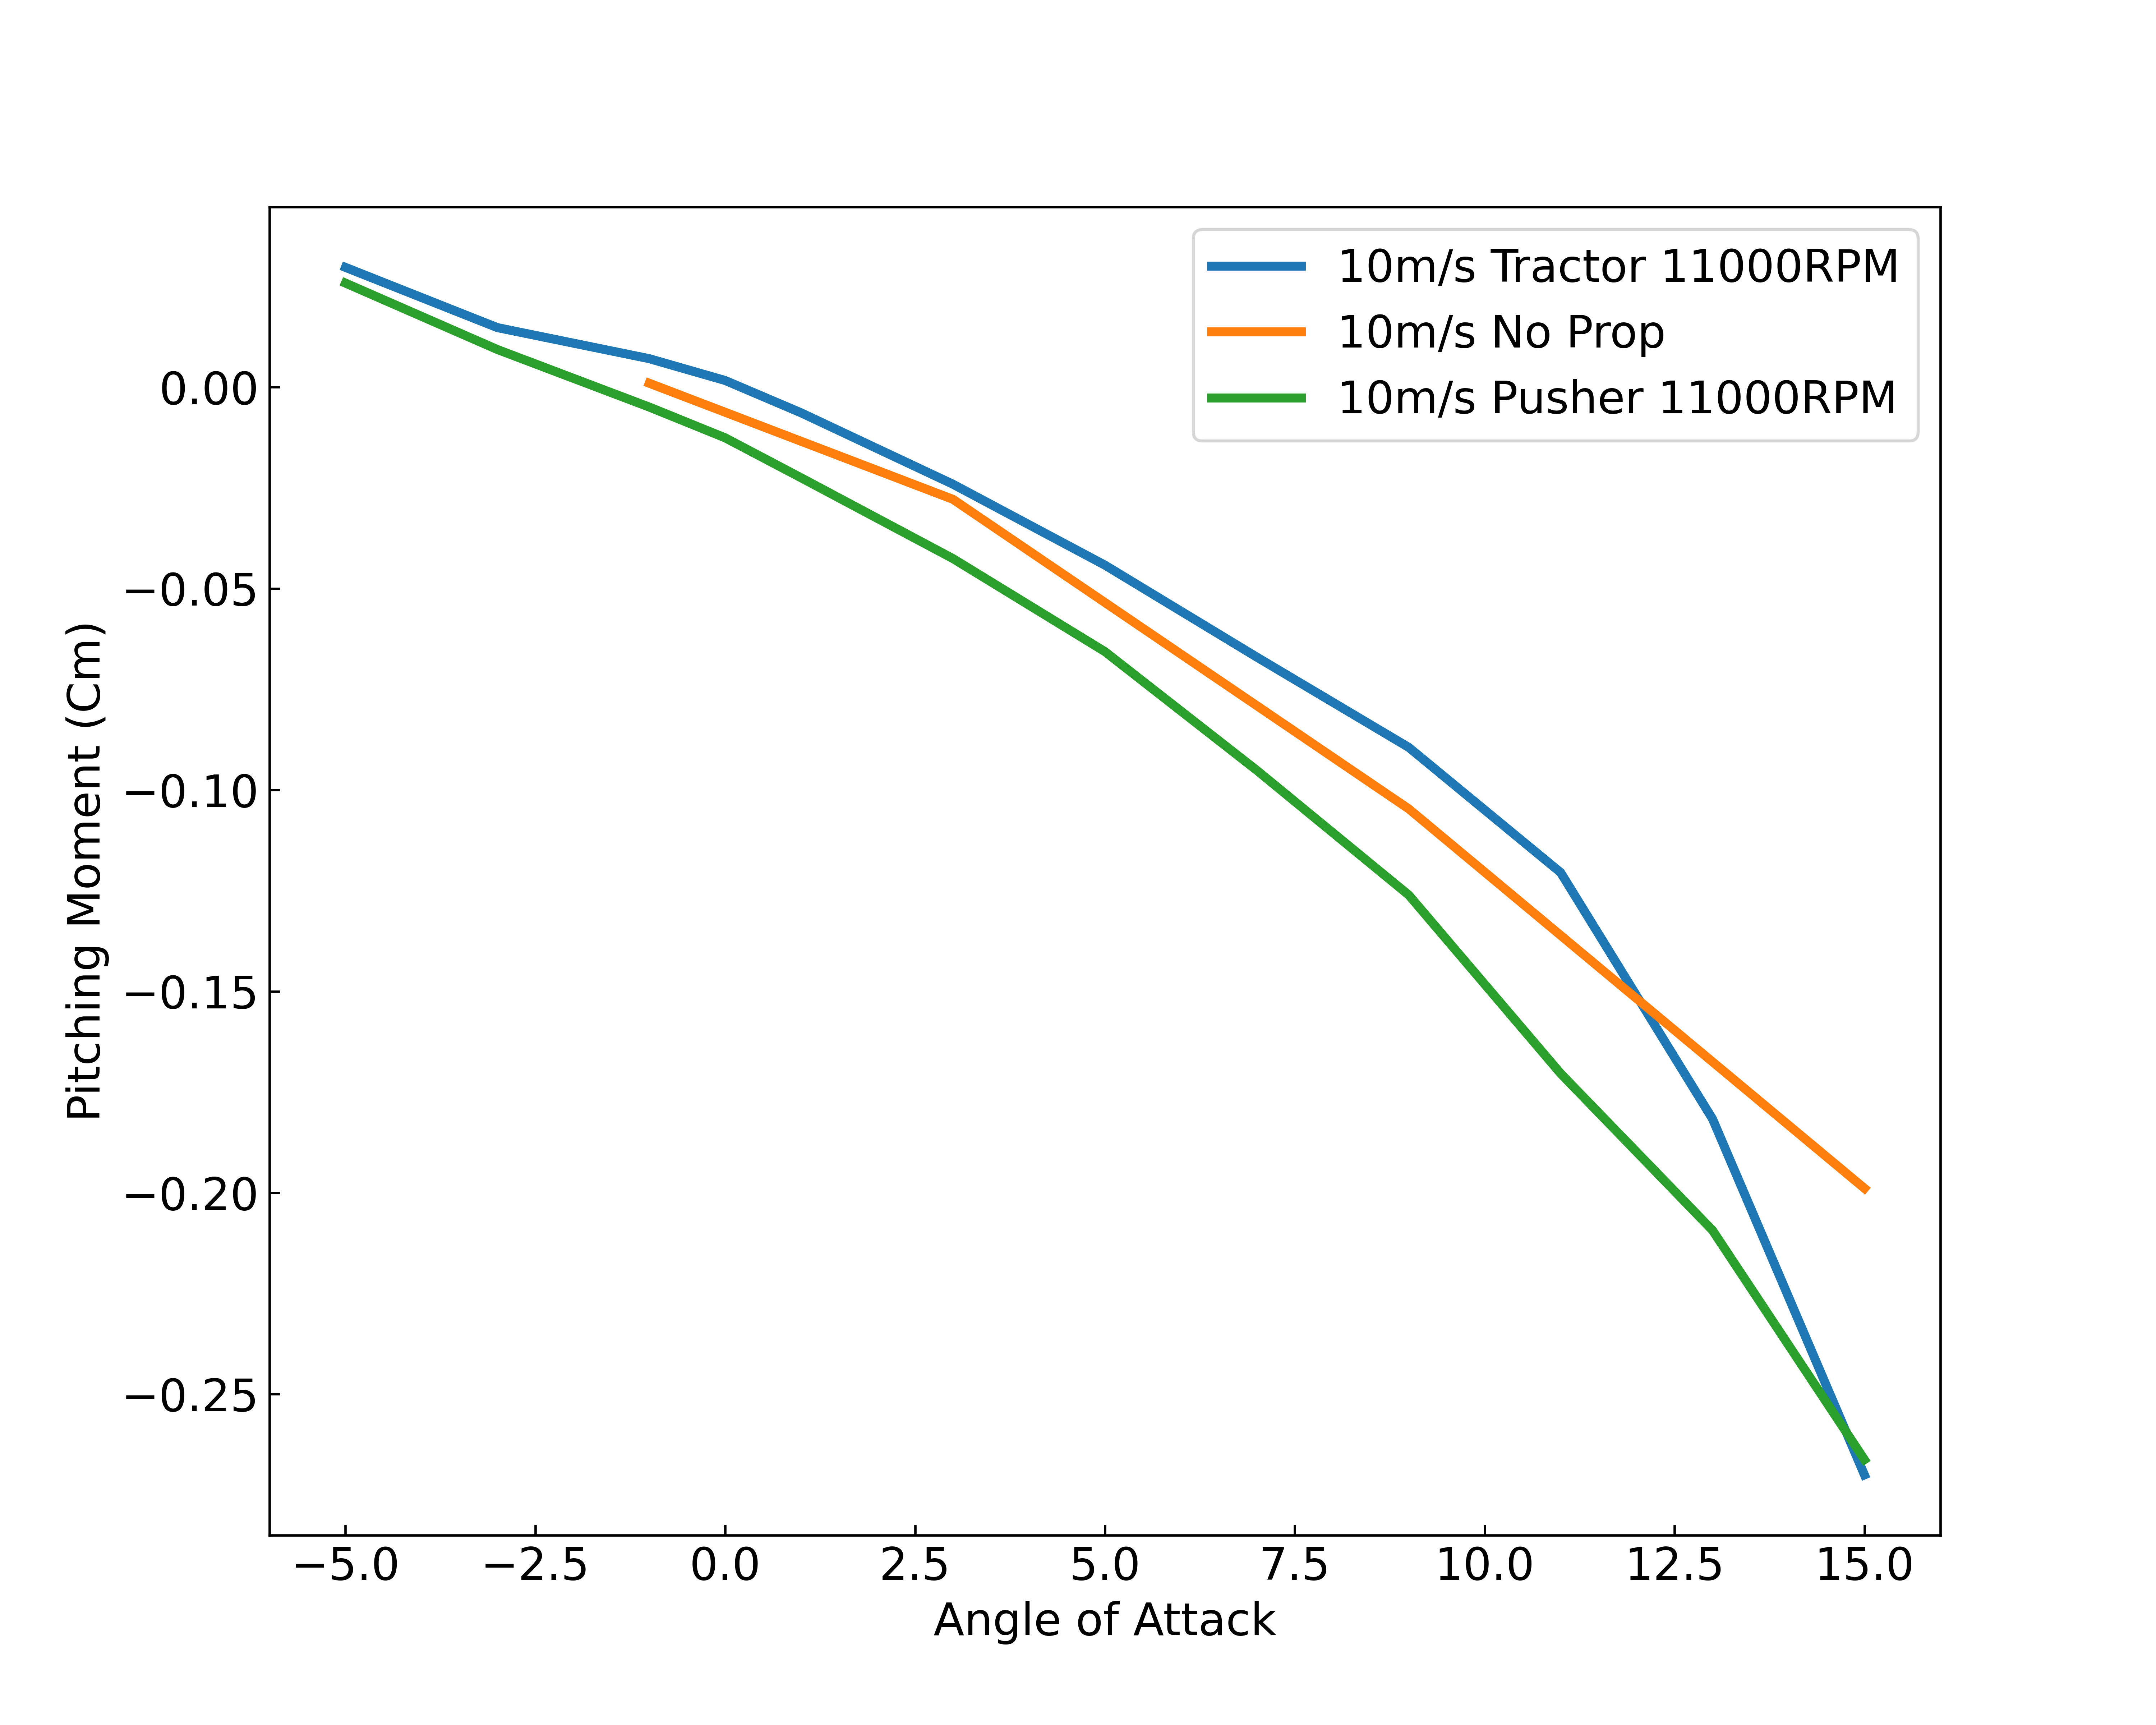
\includegraphics[width=\textwidth]{05_Results/Figs/Cm/10ms_11000RPM_Cm.png}
        \caption{Pitching Moment Coefficient at 10m/s airspeed and 11000RPM motor speed}
        \label{fig:Cm_10ms_11000}
    \end{subfigure}
    \begin{subfigure}[b]{0.467\textwidth}
        \centering
        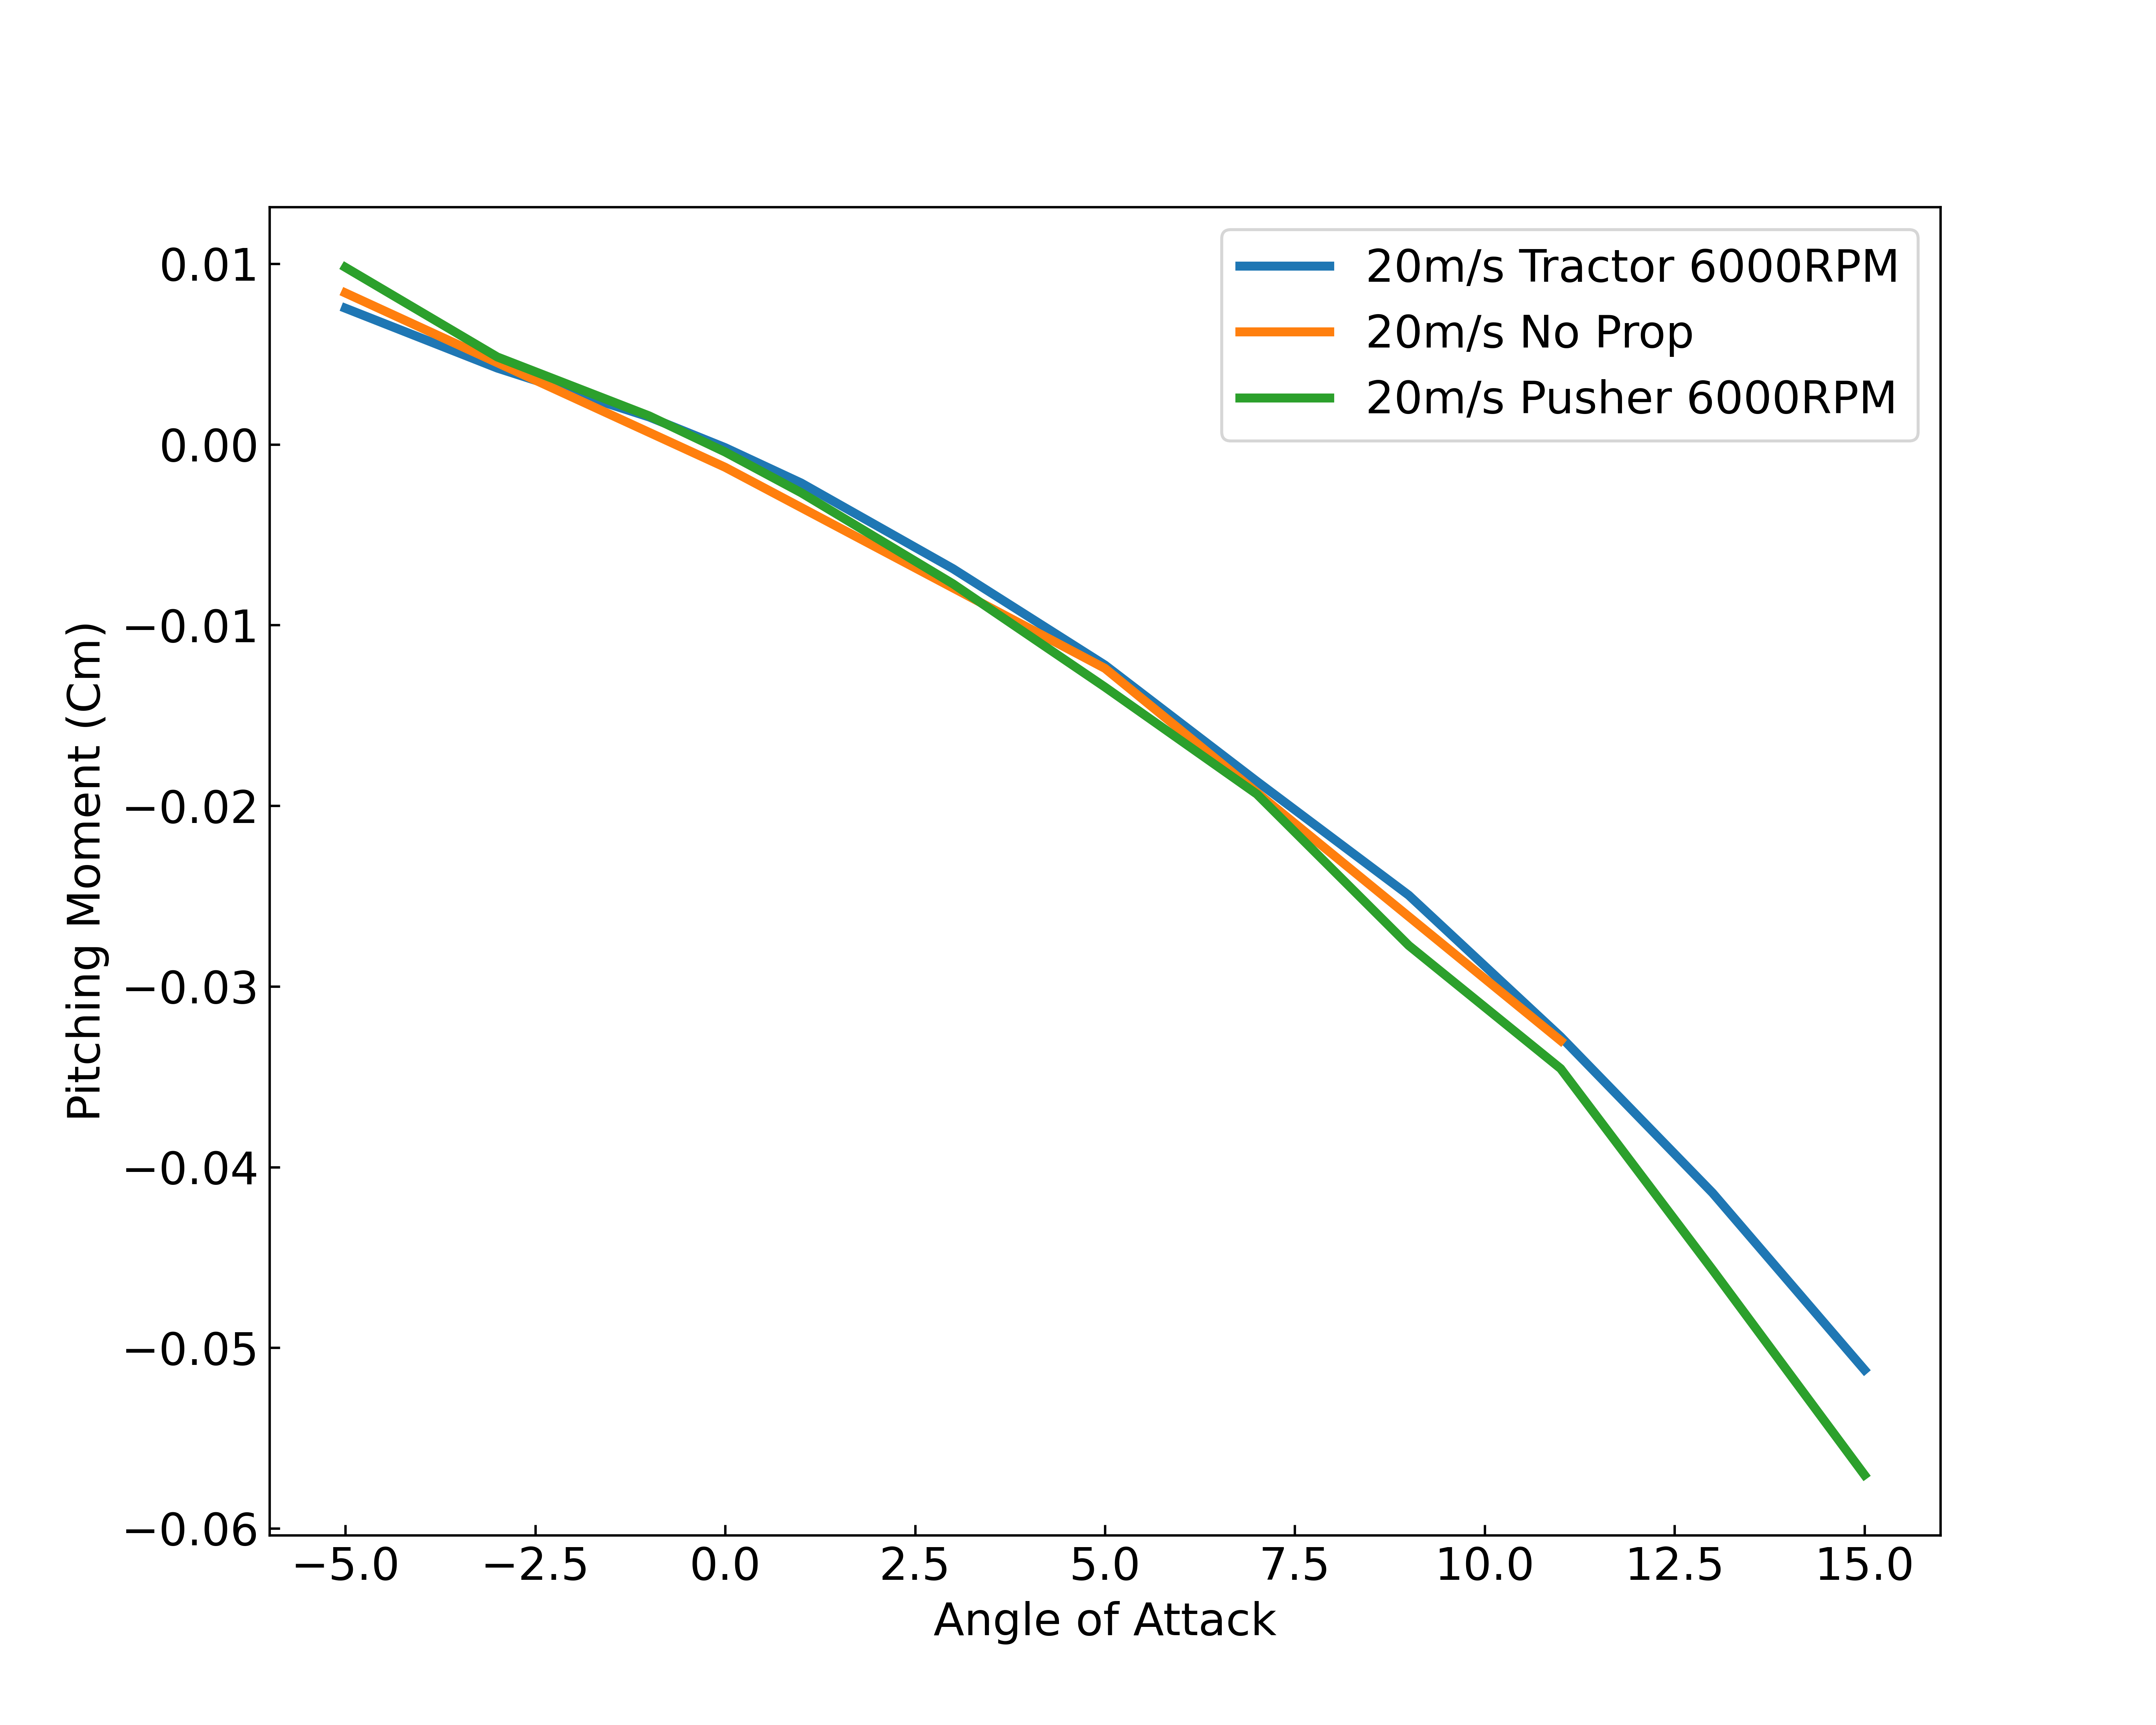
\includegraphics[width=\textwidth]{05_Results/Figs/Cm/20ms_6000RPM_Cm.png}
        \caption{Pitching Moment Coefficient at 20m/s airspeed and 6000RPM motor speed}
        \label{fig:Cm_20ms_6000}
    \end{subfigure}
    \begin{subfigure}[b]{0.467\textwidth}
        \centering
        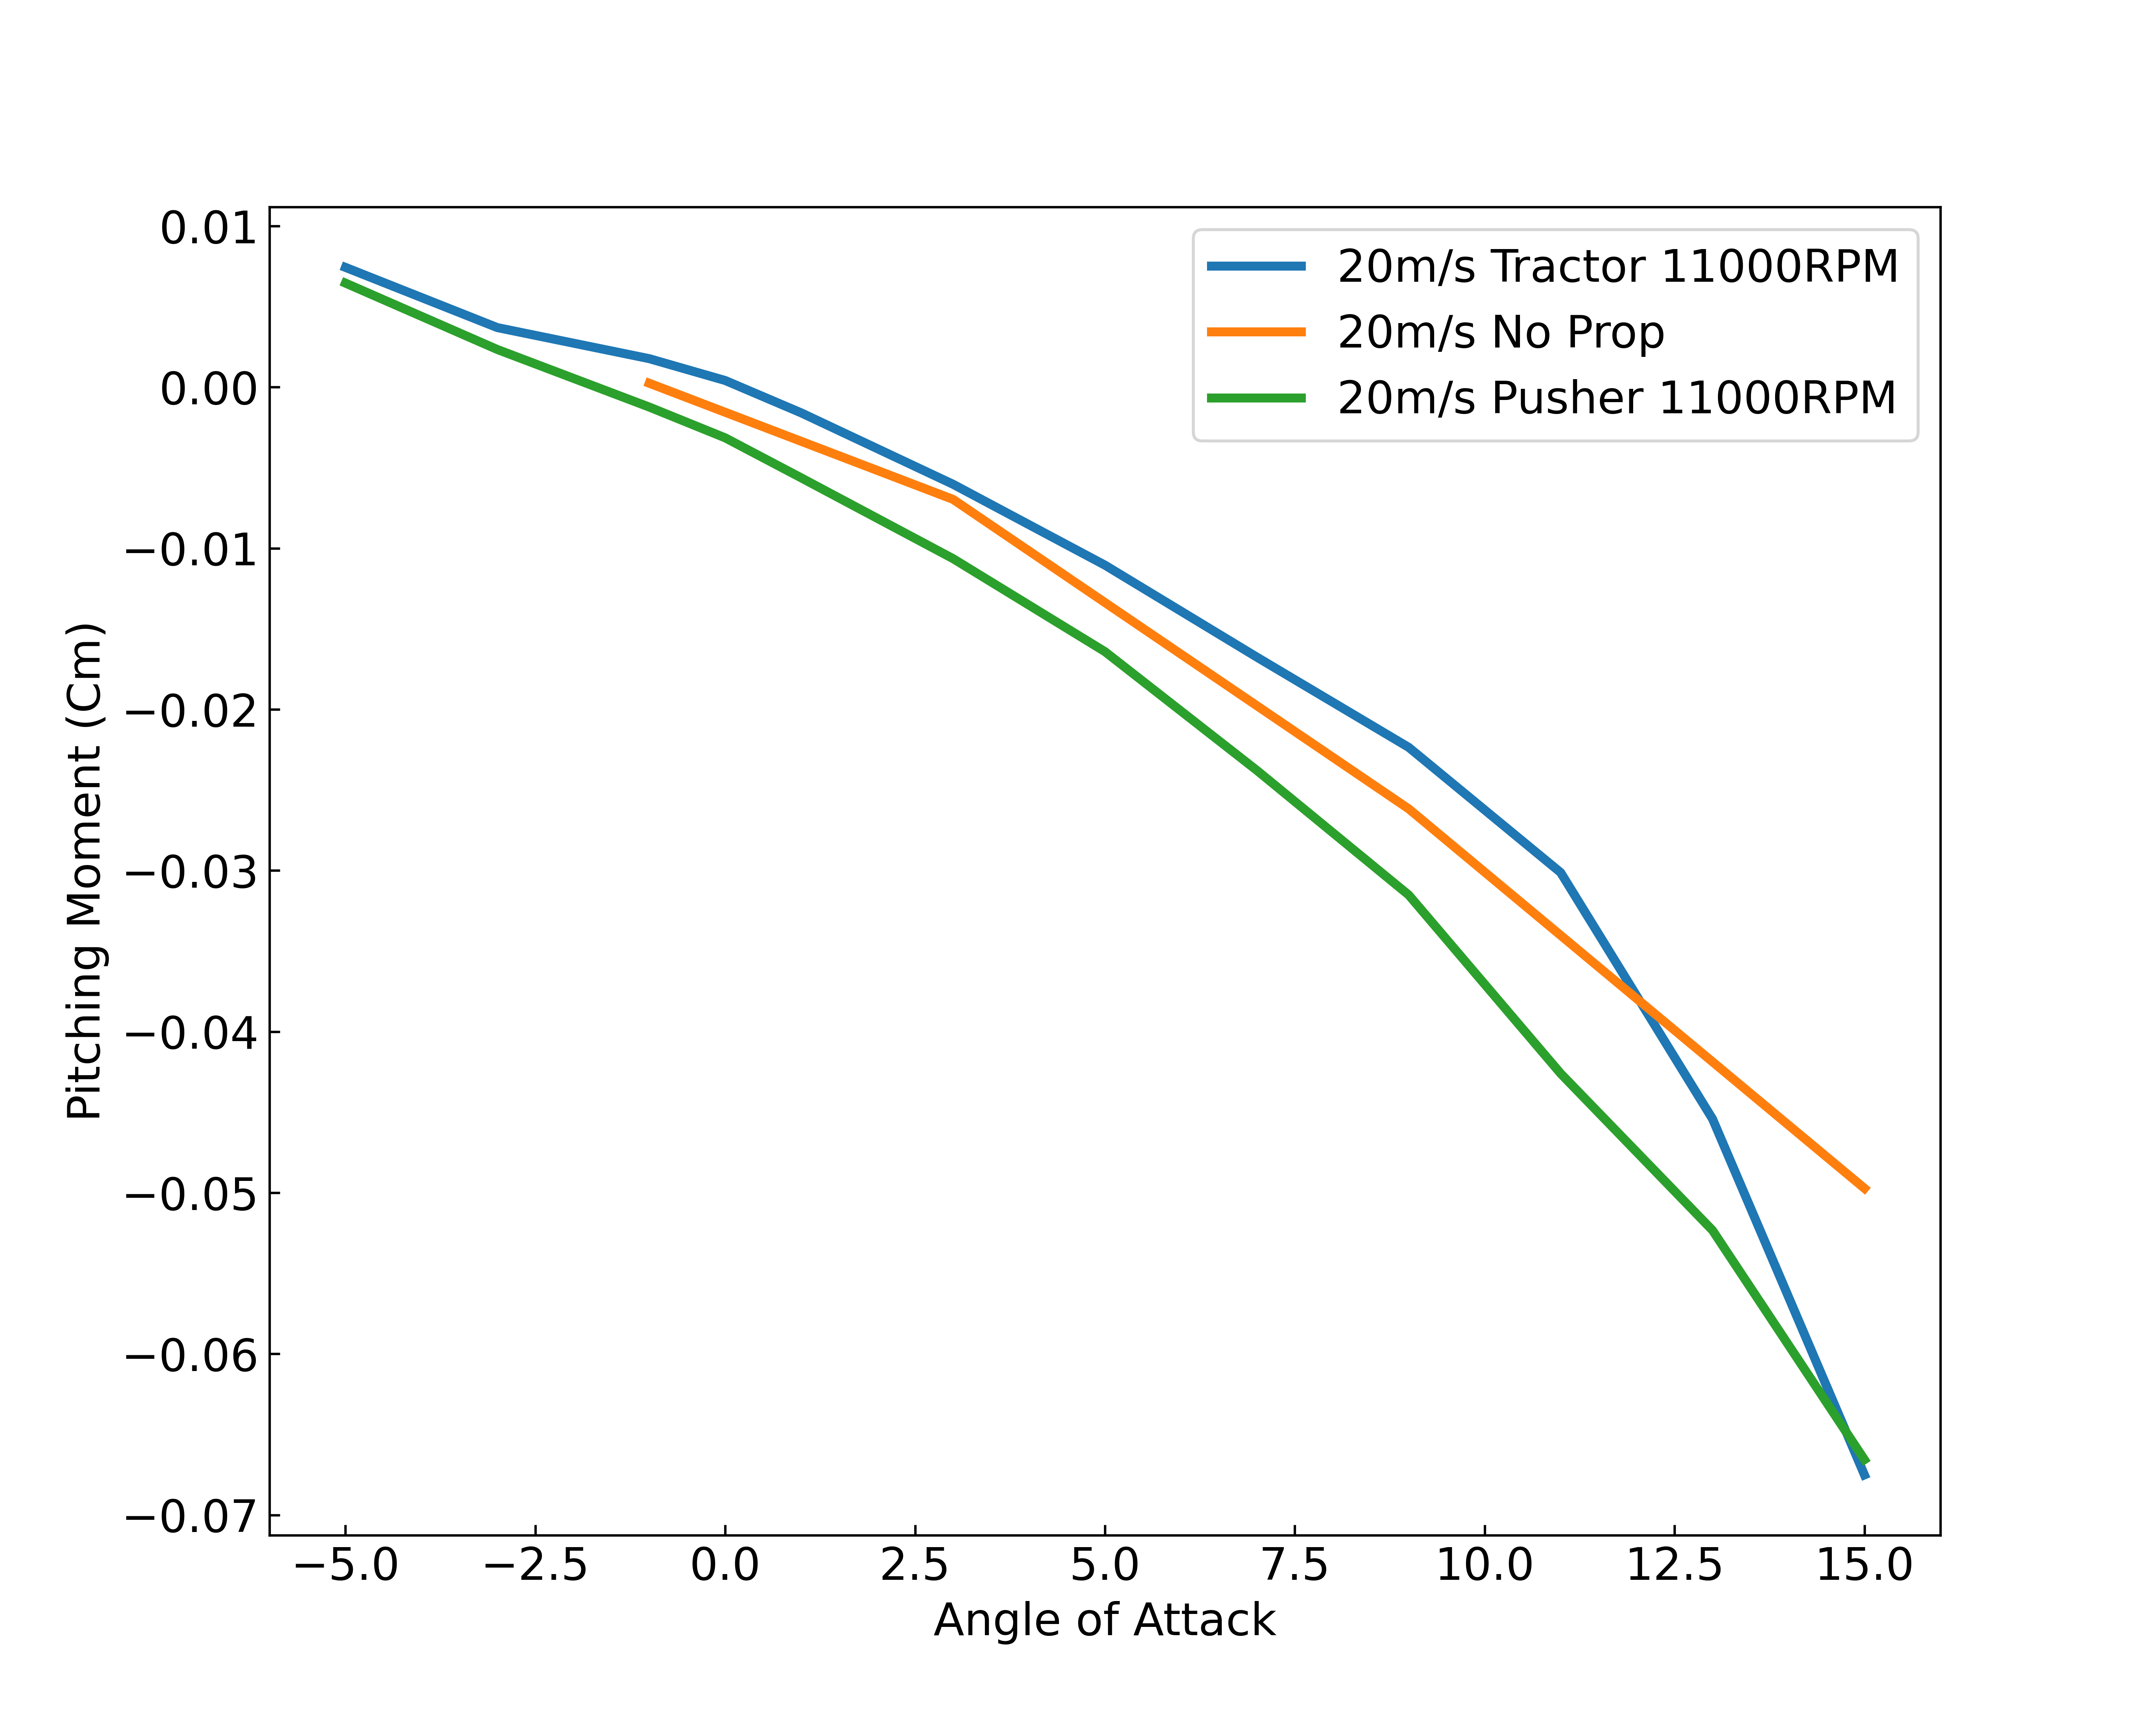
\includegraphics[width=\textwidth]{05_Results/Figs/Cm/20ms_11000RPM_Cm.png}
        \caption{Pitching Moment Coefficient at 20m/s airspeed and 11000RPM motor speed}
        \label{fig:Cm_20ms_11000}
    \end{subfigure}
    
\end{figure}

\subsection{Rolling Moment Coefficient}

Figures \ref{fig:Cl_roll_10ms_6000} to \ref{fig:Cl_roll_20ms_11000} show that the rolling moment coefficient for the tractor configuration at 6000RPM propeller speed was shifted downwards compared to both the pusher and no propeller configurations, leading to a decrease in the rolling moment for all airspeeds. At 11000RPM propeller speed, the tractor configuration did not show a significant shift downwards until a sharp drop, seen at $\approx$12.5$^{\circ}$ \acrshort{AoA}. However, the pusher configuration shows a shift upwards and an increase in the rolling coefficient for all airspeeds and propeller speeds. The rolling moment is due to the propeller torque effect due to the propeller wing interaction, previously described in Section \ref{sec:propellerWingInteraction}. The tractor configuration also experiences a flow distribution change over the wings and fuselage due to the propeller's upwash and downwash effect, as described in Section \ref{sec:propellerWingInteraction}. These propeller effects affect the lift distribution across the wings' surface, shifting the roll moment coefficient upwards as one wing is in the upwash of the propeller blades and the other in the downwash airstream. As the \acrshort{AoA} increases, the rolling moment increases until sharply dropping off as the right wing of the \acrshort{MAV} stalled first, creating a lift force imbalance as the left wing continued to produce lift. At the same time, the right-wing experiences flow separation due to stalling. The rolling moment sharply raises as the left wing also stalls and the flow over the left wing separates. The pusher configuration shifts the rolling moment to a larger extent due to having a larger moment arm from the position of the propeller to the aerodynamic centre of the \acrshort{MAV} model than the tractor configuration. The pusher configuration also shows an increase in the roll moment coefficient at 0$^{\circ}$ \acrshort{AoA} for all airspeeds, while the tractor configuration shows this only when the propeller is running at 11000RPM. The rolling moment also decreases after 2.5$^{\circ}$ \acrshort{AoA} for the tractor configuration when the propeller runs at 11000RPM. The increases in roll moment at 0$^{\circ}$ \acrshort{AoA} is likely due to an interaction with the wing and/or the wings wake. However, more investigation is needed to validate this.  

\begin{figure}[H]
    \centering
    \begin{subfigure}[b]{0.467\textwidth}
        \centering
        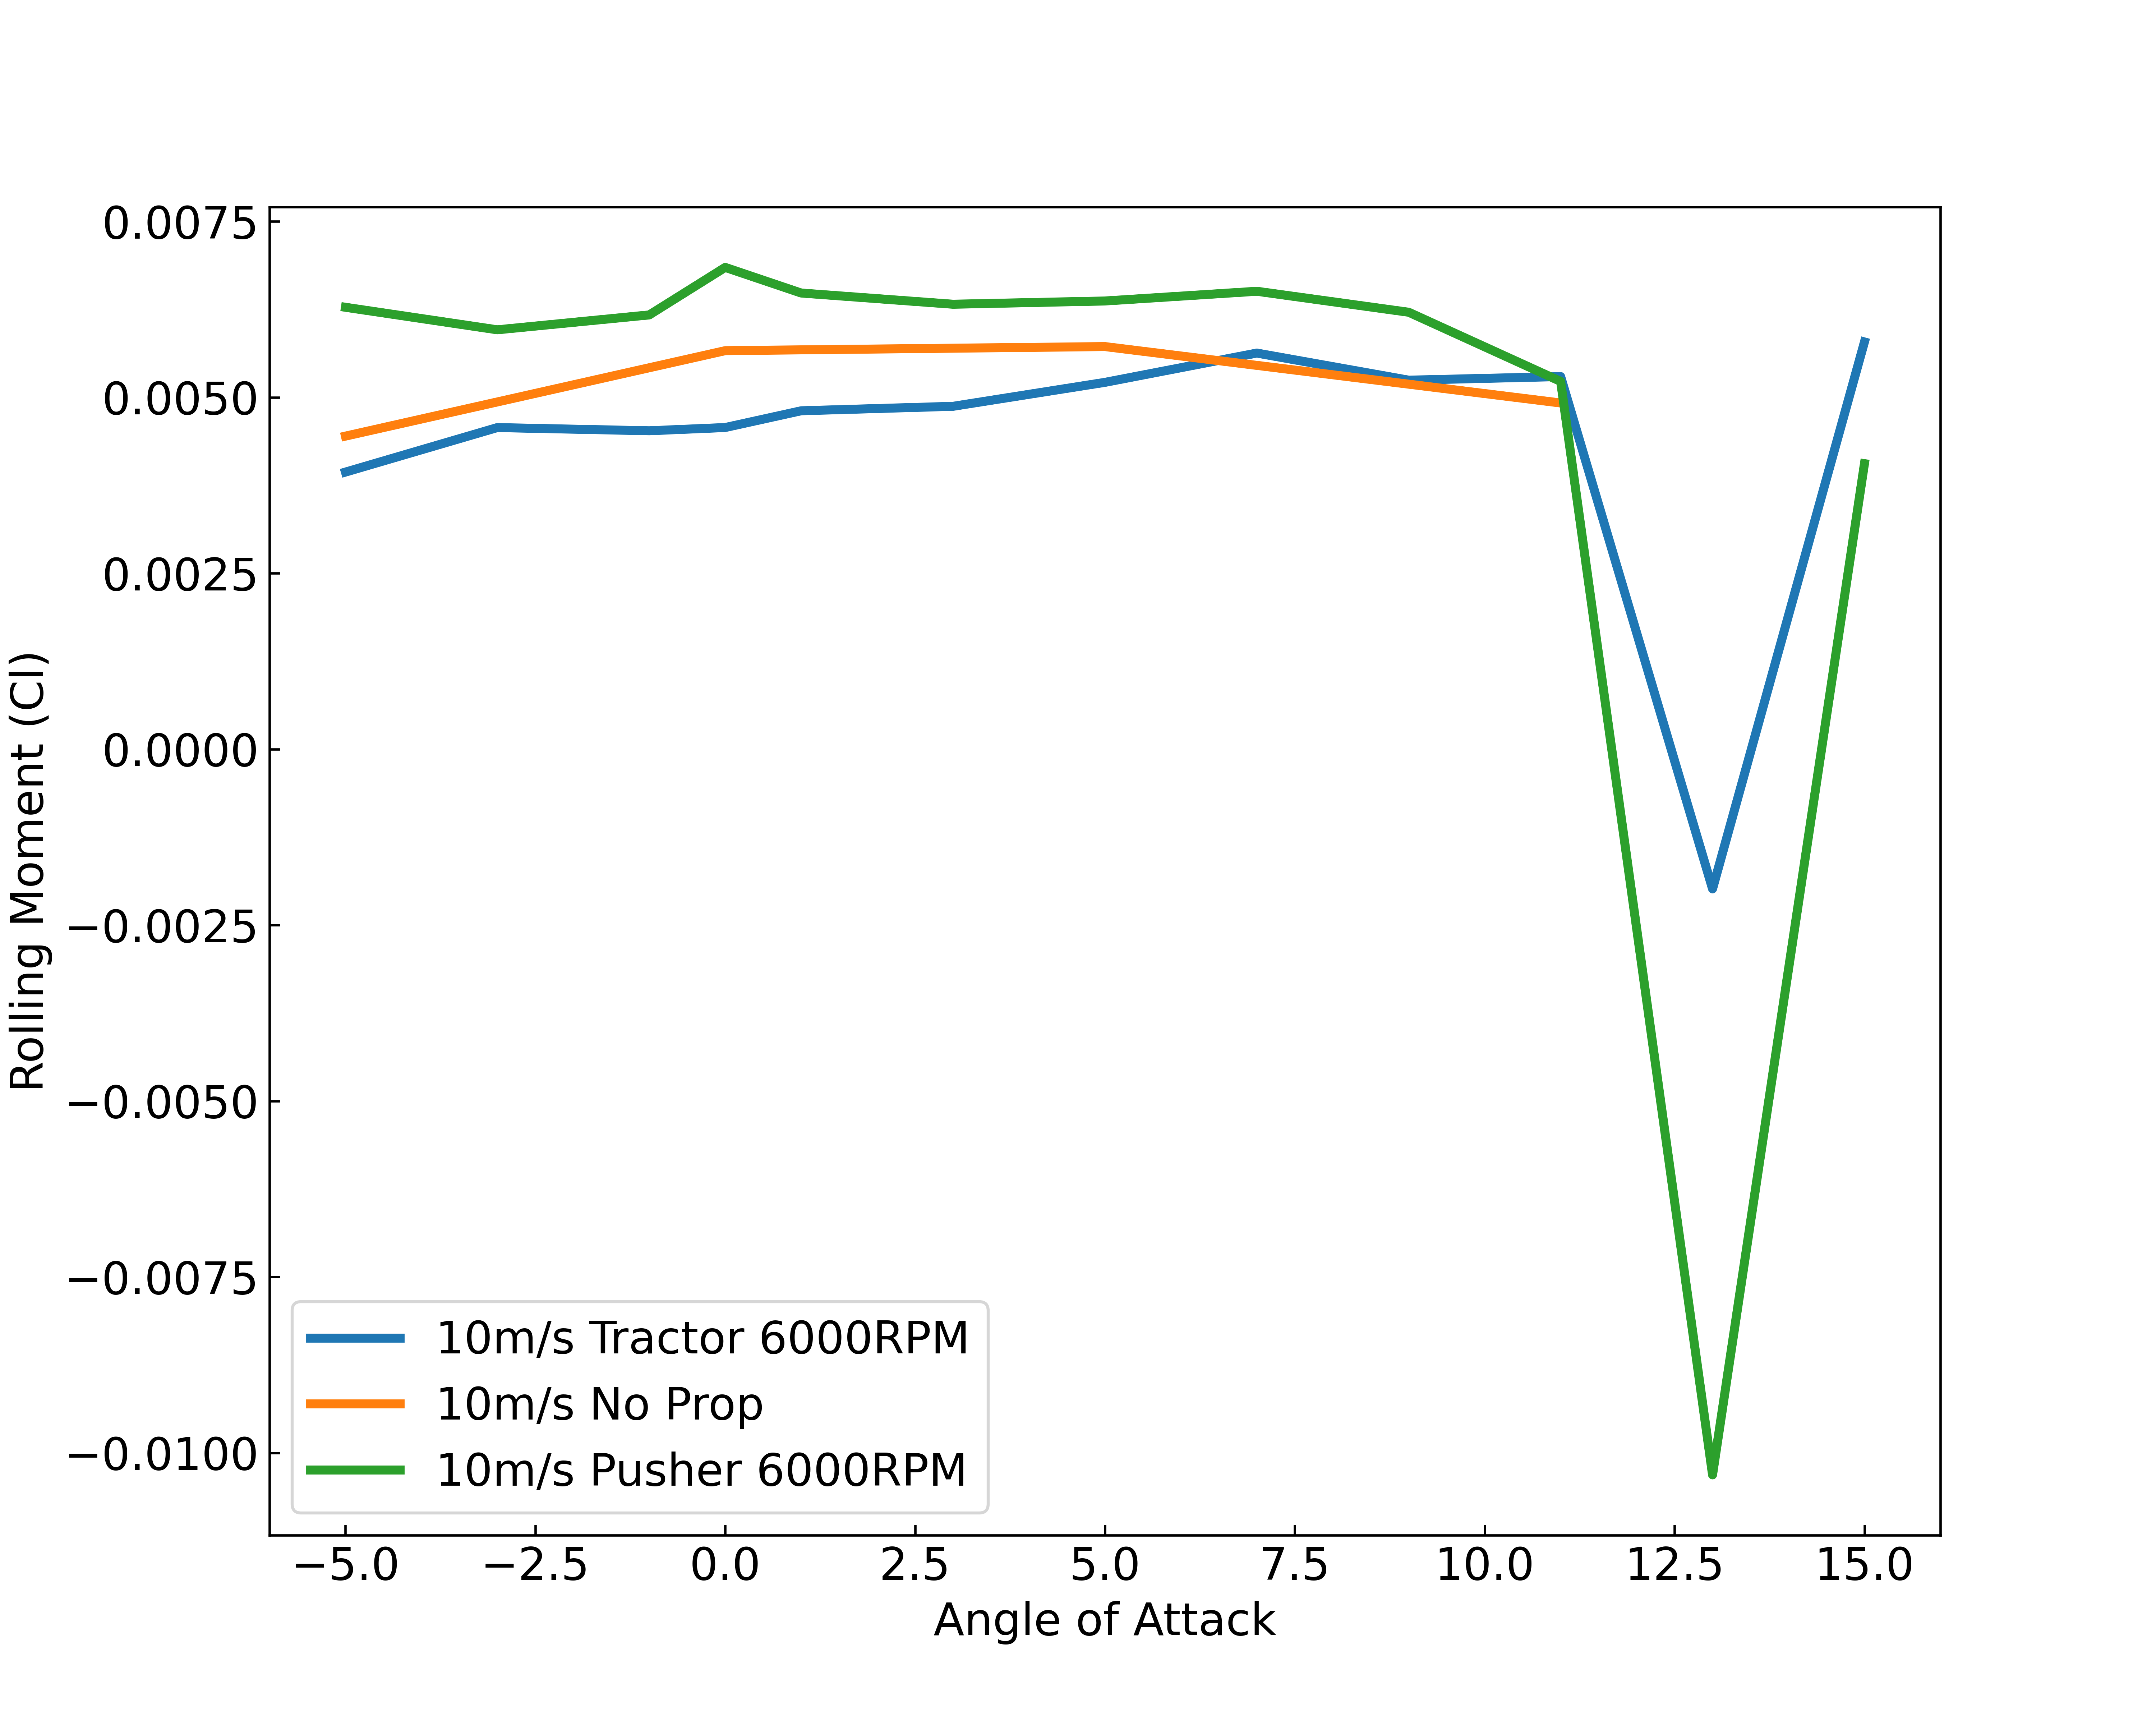
\includegraphics[width=0.8\textwidth]{05_Results/Figs/Cl_roll/10ms_6000RPM_Cl_roll.png}
        \caption{Rolling Moment Coefficient at 10m/s airspeed and 6000RPM motor speed}
        \label{fig:Cl_roll_10ms_6000}
    \end{subfigure}
    \begin{subfigure}[b]{0.467\textwidth}
        \centering
        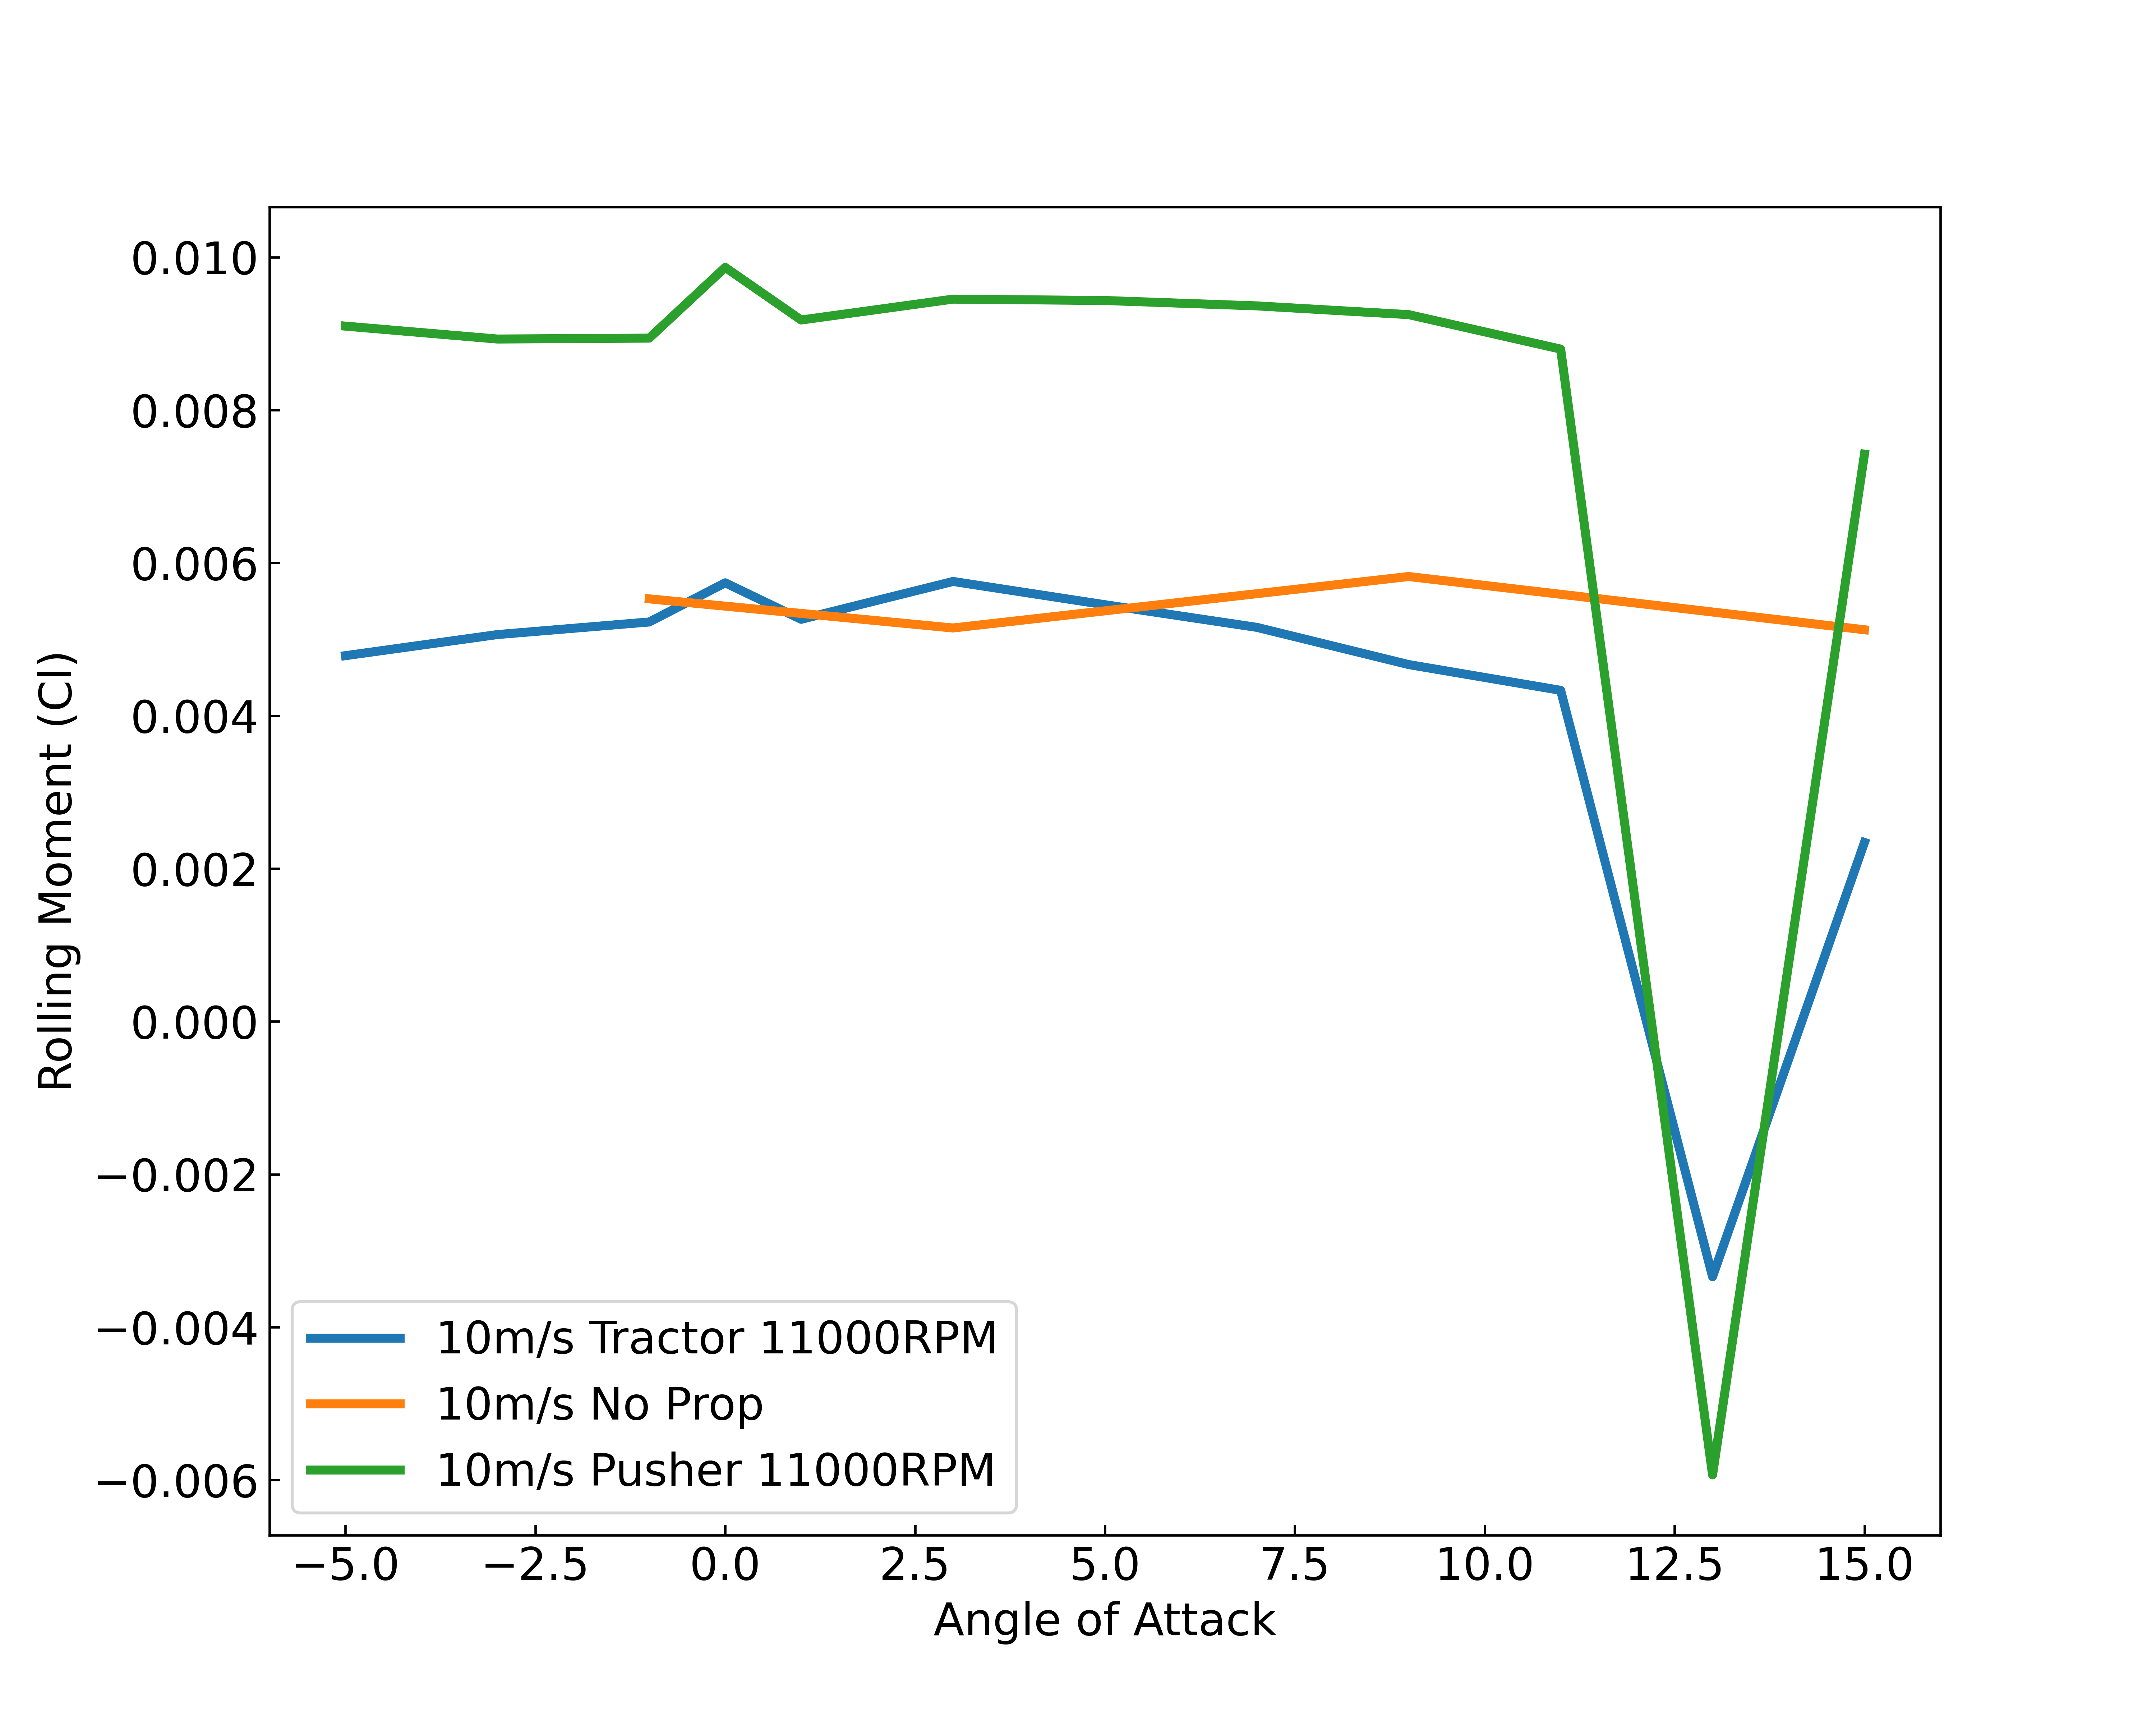
\includegraphics[width=0.8\textwidth]{05_Results/Figs/Cl_roll/10ms_11000RPM_Cl.png}
        \caption{Rolling Moment Coefficient at 10m/s airspeed and 11000RPM motor speed}
        \label{fig:Cl_roll_10ms_11000}
    \end{subfigure}
\end{figure}

\begin{figure}[H]\ContinuedFloat
    \begin{subfigure}[b]{0.467\textwidth}
        \centering
        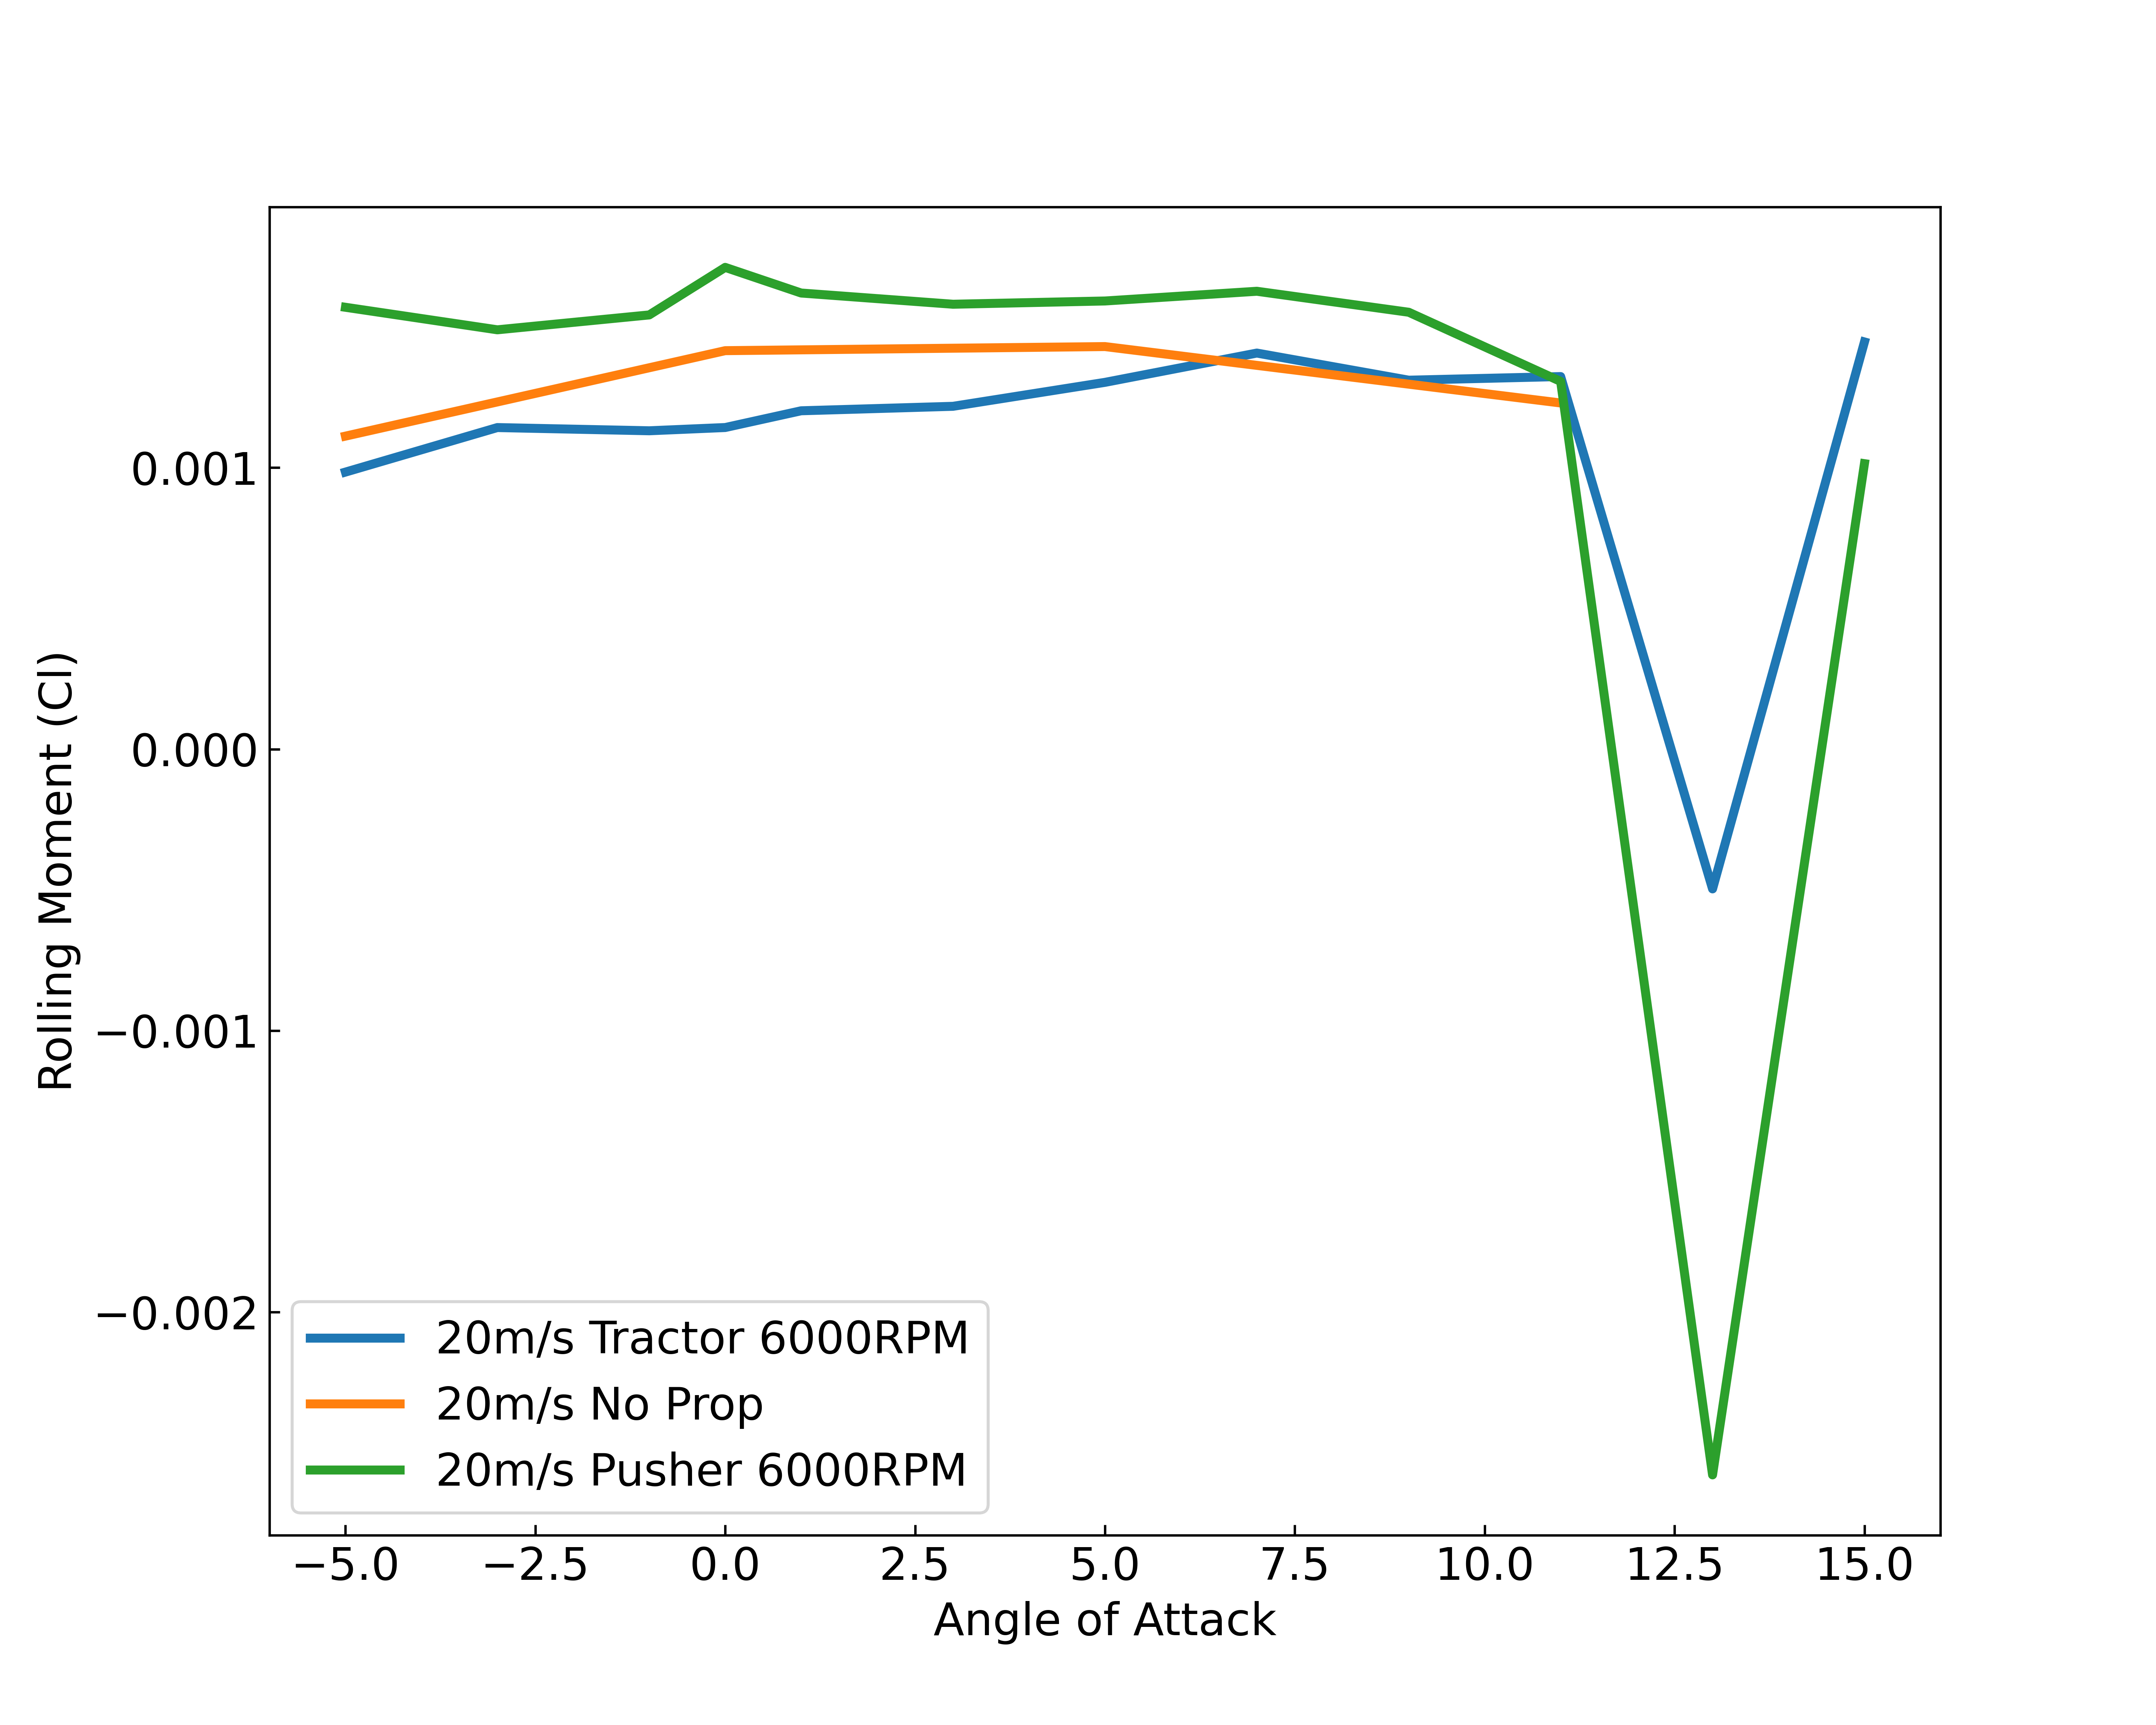
\includegraphics[width=0.8\textwidth]{05_Results/Figs/Cl_roll/20ms_6000RPM_Cl_roll.png}
        \caption{Rolling Moment Coefficient at 20m/s airspeed and 6000RPM motor speed}
        \label{fig:Cl_roll_20ms_6000}
    \end{subfigure}
    \begin{subfigure}[b]{0.467\textwidth}
        \centering
        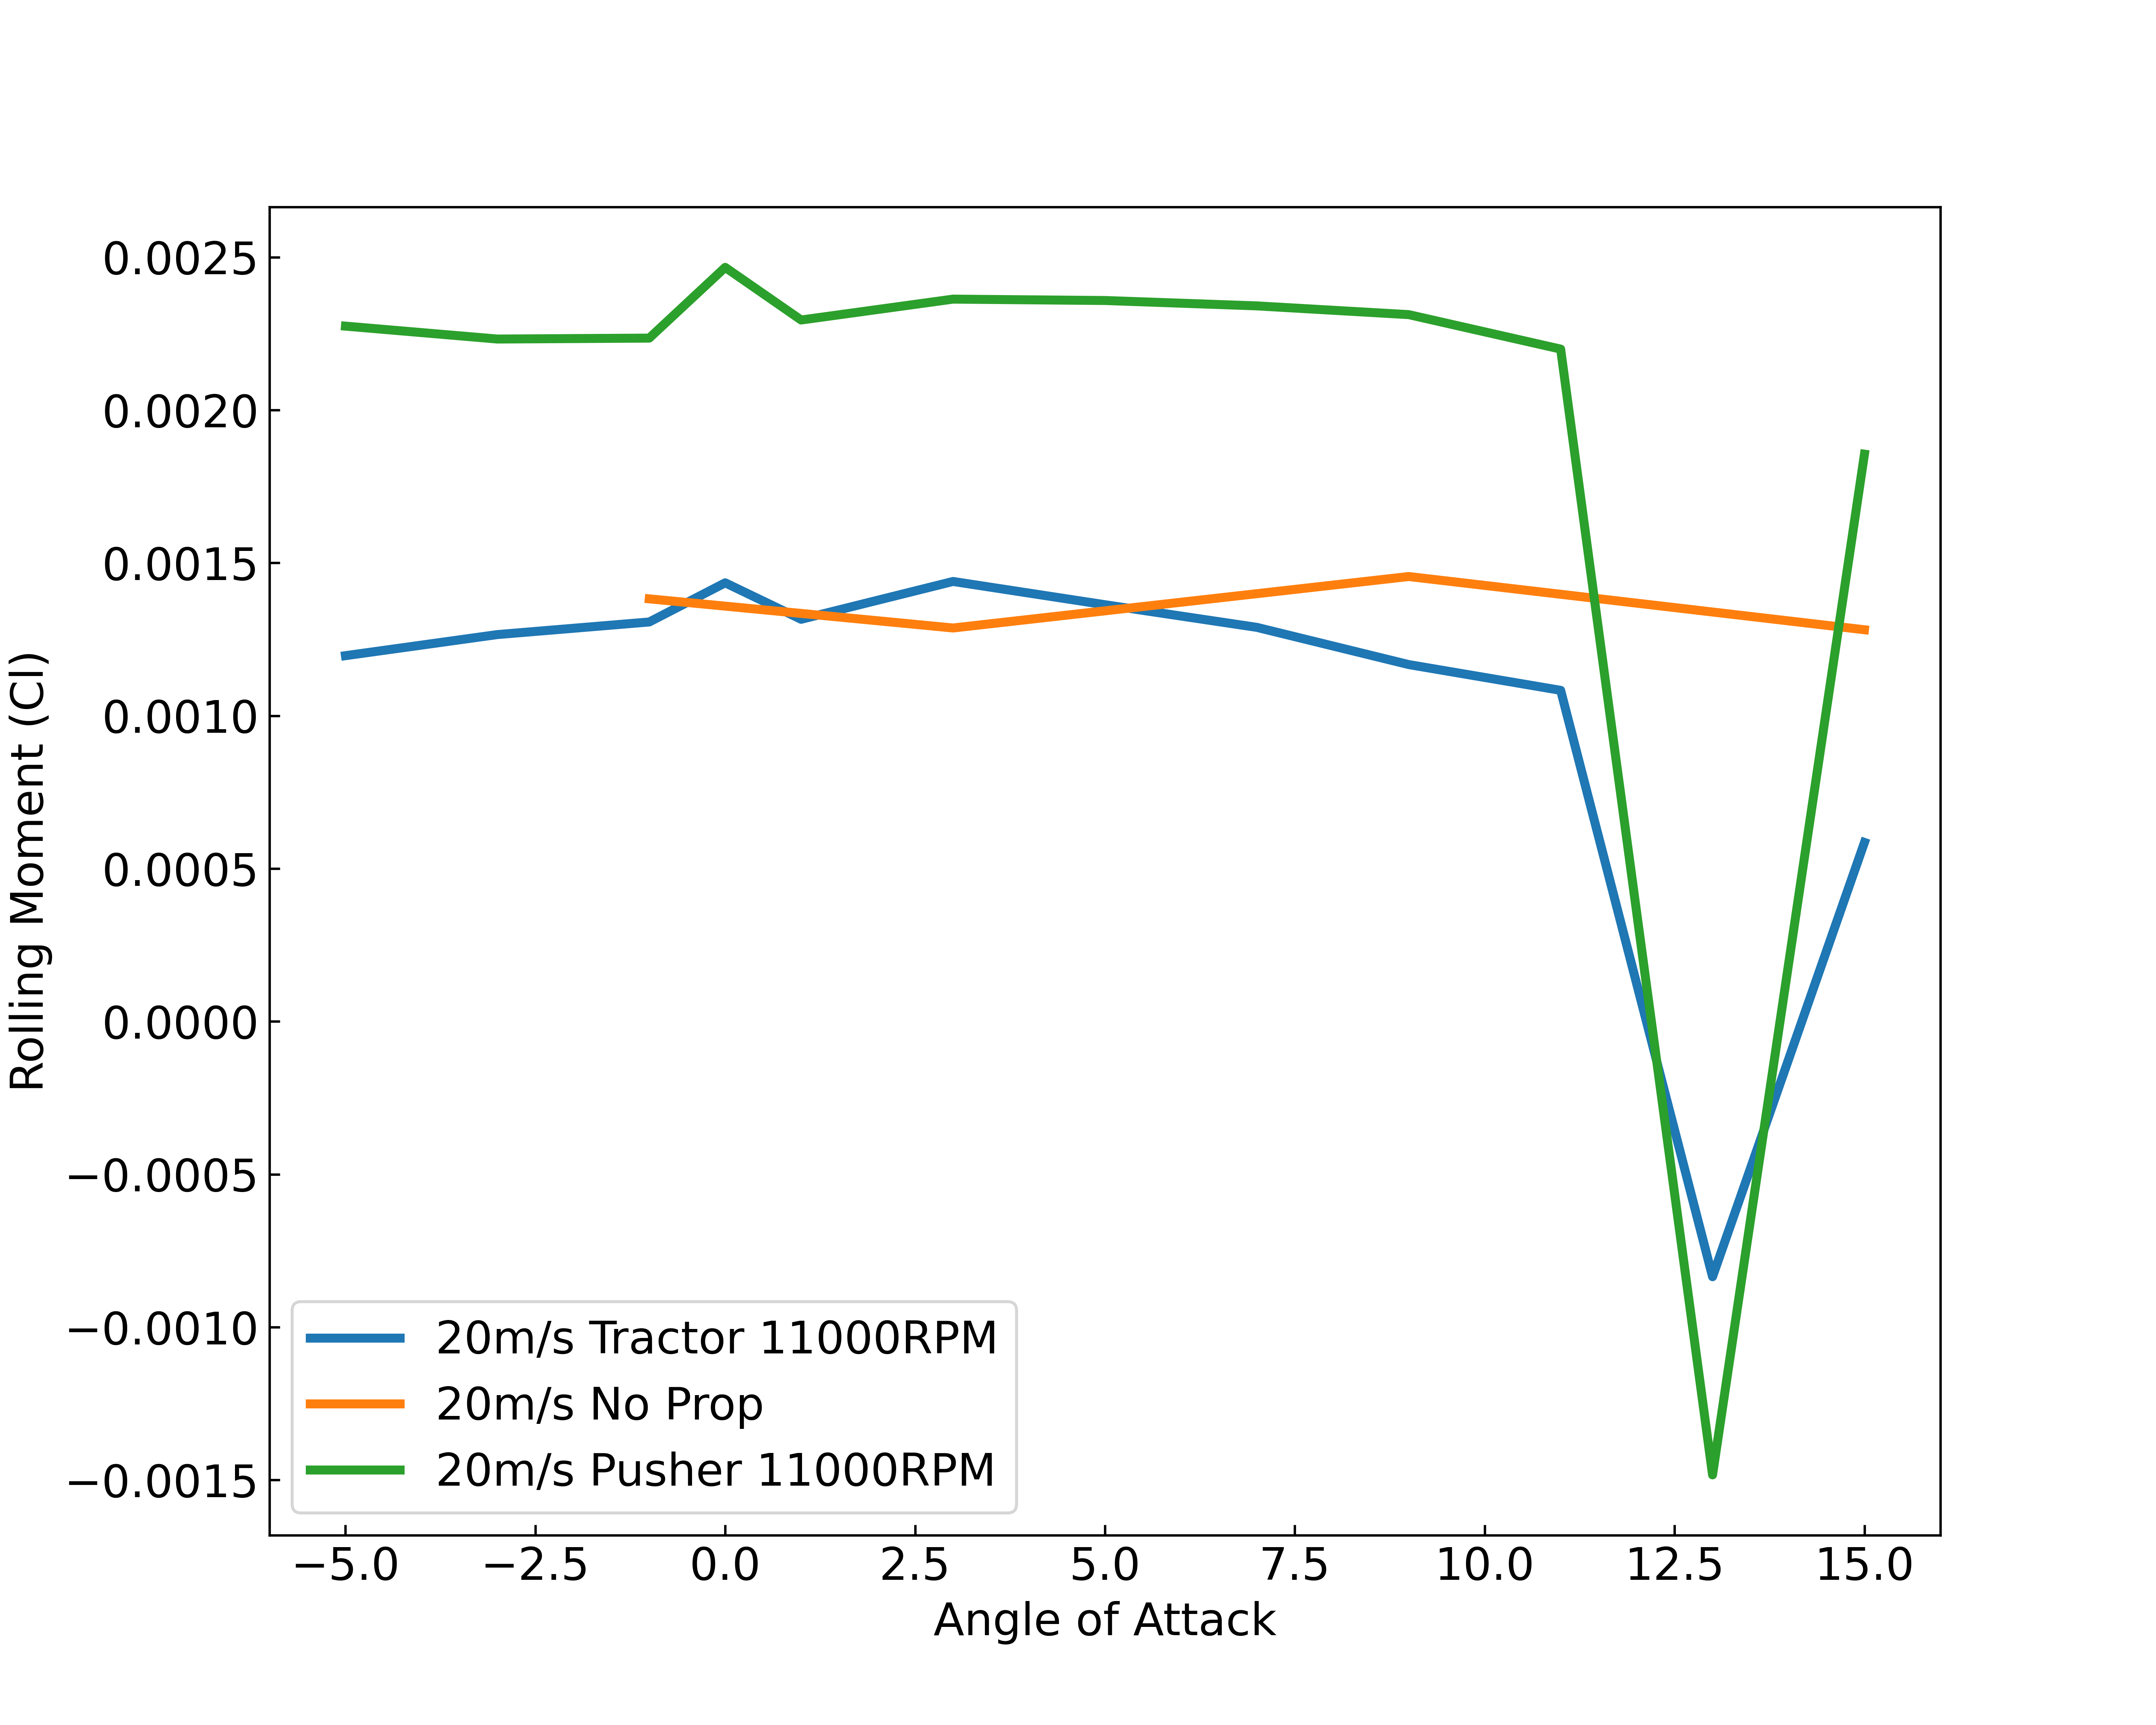
\includegraphics[width=0.8\textwidth]{05_Results/Figs/Cl_roll/20ms_11000RPM_Cl.png}
        \caption{Rolling Moment Coefficient at 20m/s airspeed and 11000RPM motor speed}
        \label{fig:Cl_roll_20ms_11000}
    \end{subfigure}
\end{figure}


\subsection{Yawing Moment Coefficient}
 Figures \ref{fig:Cl_roll_10ms_6000} to \ref{fig:Cl_roll_20ms_11000} show that the yaw coefficient for the tractor configuration was shifted upwards compared to the pusher and no propeller configurations. The yawing moment is produced as a consequence of the roll moment. The aircraft roll moment remains relatively constant until the stall of the right wing at $\approx$12.5$^{\circ}$ \acrshort{AoA}. Hence the increase in the yawing moment as the aircraft \acrshort{AoA} increases is likely due to the effects of the roll being magnified as flow separation occurs. The roll moment causes an adverse yaw effect where the \acrshort{MAV} naturally tends to yaw in the opposite direction of the roll \cite{Arivoli2011}. This is due to the different lift and drag acting on each wing. As the angle of attack increases, the difference between the two wings in lift and drag increases, leading to an increase in the yaw moment for all configurations, airspeeds and propeller speeds except for the no propeller configuration when run at 20m$s^{-1}$. As the angle of attack increases, the yaw moment increases until sharply dropping off in Figures \ref{fig:Cl_roll_10ms_6000} to \ref{fig:Cl_roll_20ms_11000}. This is also due to the stall of the right-wing, creating a lift force imbalance as the left wing continues to produce a lift force while the right-wing experiences flow separation due to the increase in \acrshort{AoA}. The yawing moment also sharply raises as the flow over the left wing also separates and stalls beyond $\approx$12.5$^{\circ}$ \acrshort{AoA}. Several kinks are seen in Figures \ref{fig:Cl_roll_10ms_6000} to \ref{fig:Cl_roll_20ms_11000}, the most notable being the changes in gradient seen for the pusher configuration with a propeller speed of 6000RPM in Figures \ref{fig:Cl_roll_10ms_6000} and \ref{fig:Cl_roll_20ms_6000} at $\approx$0$^{\circ}$, $\approx$2.5$^{\circ}$ and $\approx$7.5$^{\circ}$\acrshort{AoA}. These changes can be partially attributed to the roll moment changes seen in Figures \ref{fig:Cl_roll_10ms_6000} to \ref{fig:Cl_roll_20ms_11000}, which creates an adverse yaw effect that acts opposite to the roll. 

\begin{figure}[H]
    \centering
    \begin{subfigure}[b]{0.467\textwidth}
        \centering
        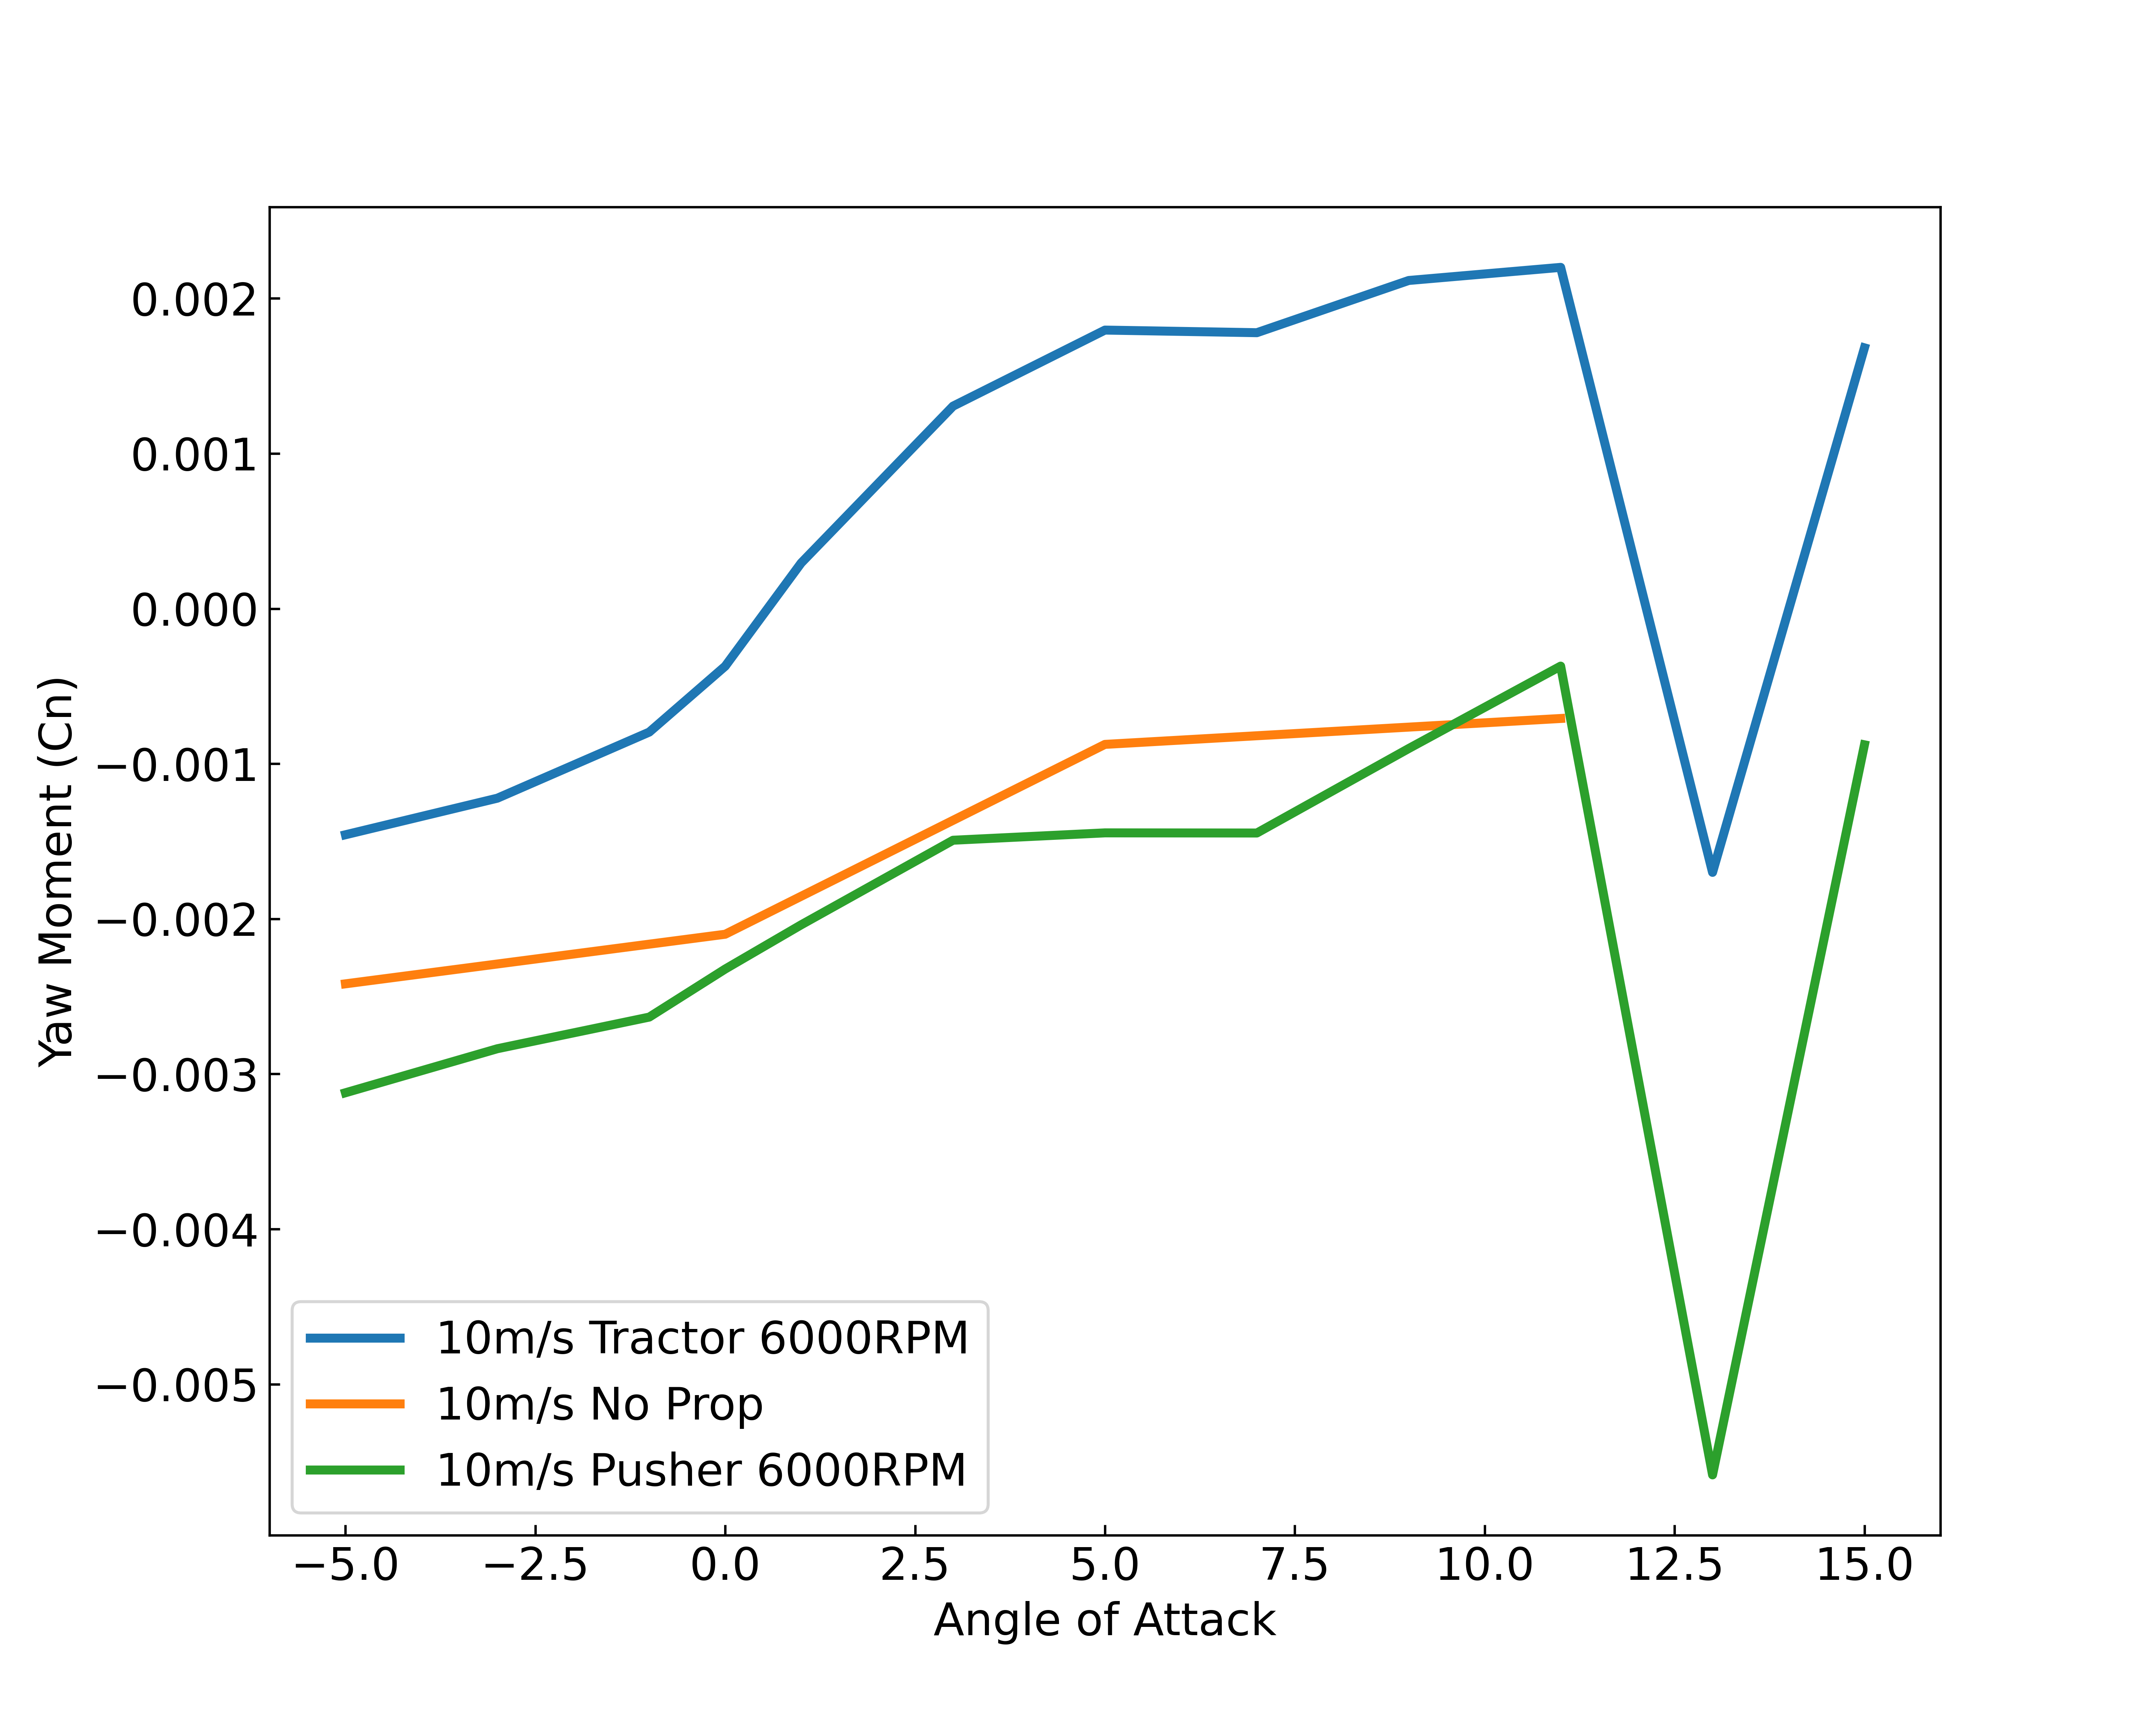
\includegraphics[width=\textwidth]{05_Results/Figs/Cn/10ms_6000RPM_Cn.png}
        \caption{Yawing Moment Coefficient at 10m/s airspeed and 6000RPM motor speed}
        \label{fig:Cn_10ms_6000}
    \end{subfigure}
    \begin{subfigure}[b]{0.467\textwidth}
        \centering
        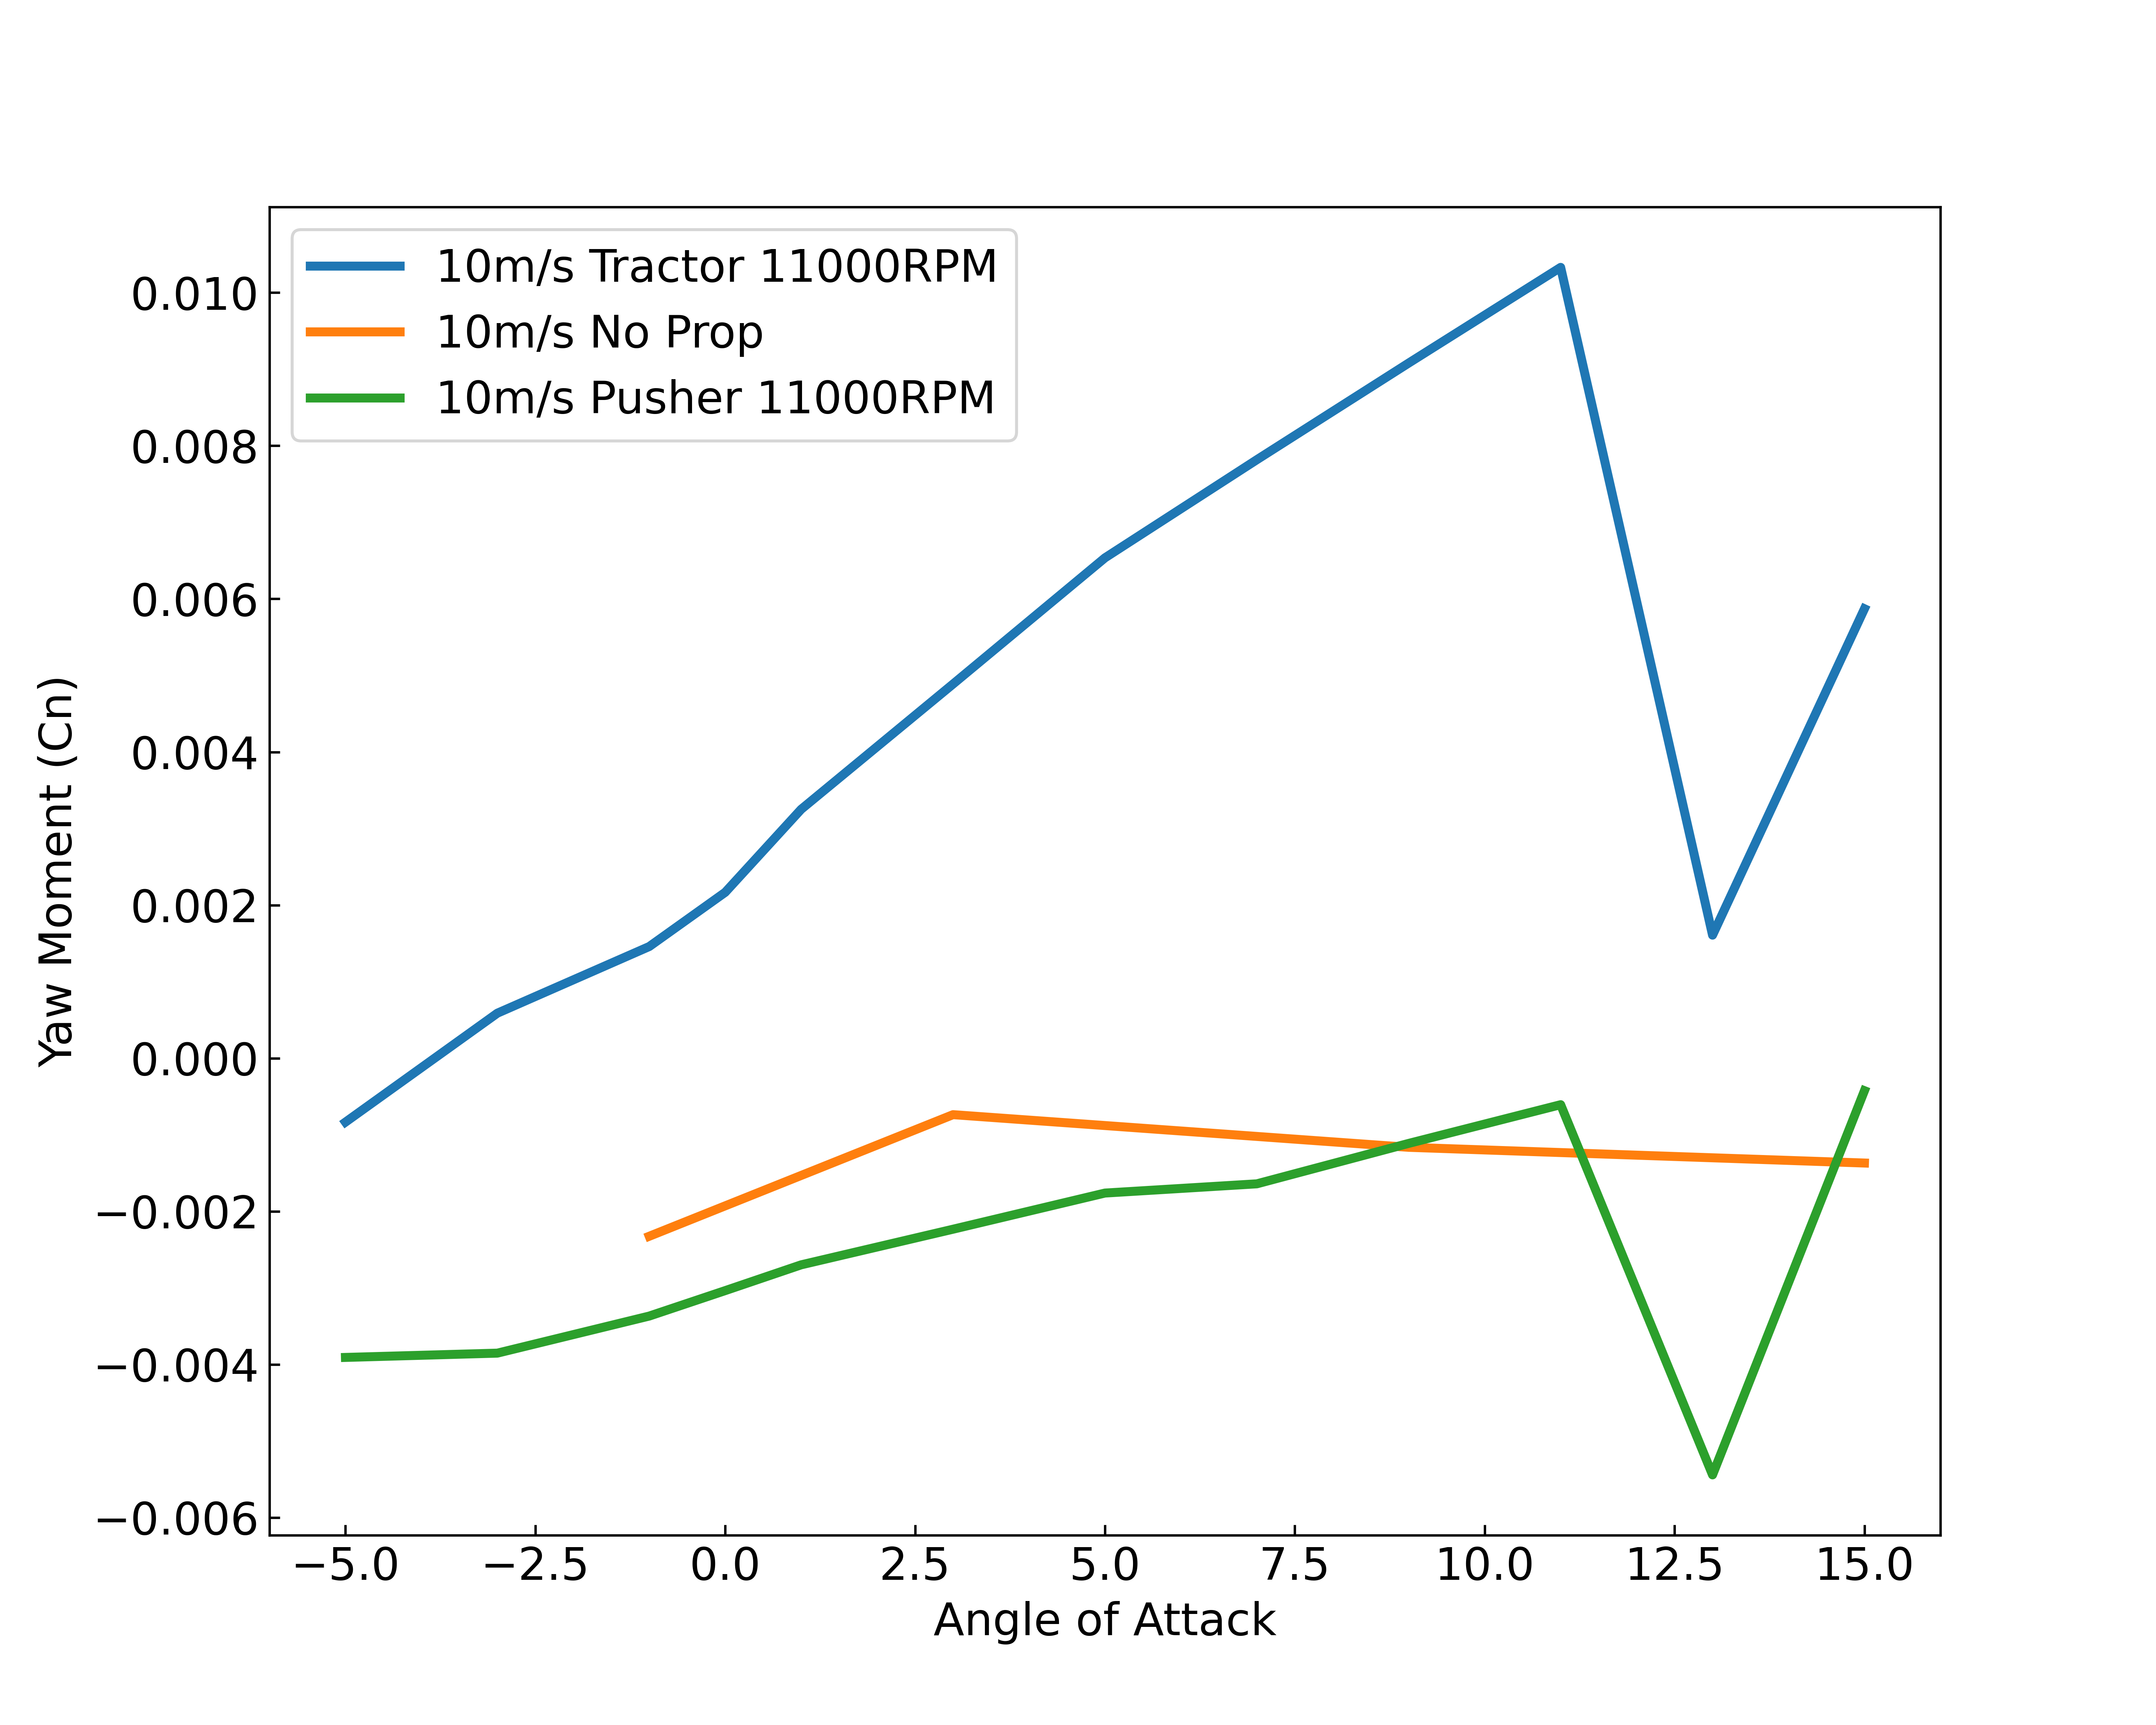
\includegraphics[width=\textwidth]{05_Results/Figs/Cn/10ms_11000RPM_Cn.png}
        \caption{Yawing Moment Coefficient at 10m/s airspeed and 11000RPM motor speed}
        \label{fig:Cn_10ms_11000}
    \end{subfigure}
    \begin{subfigure}[b]{0.467\textwidth}
        \centering
        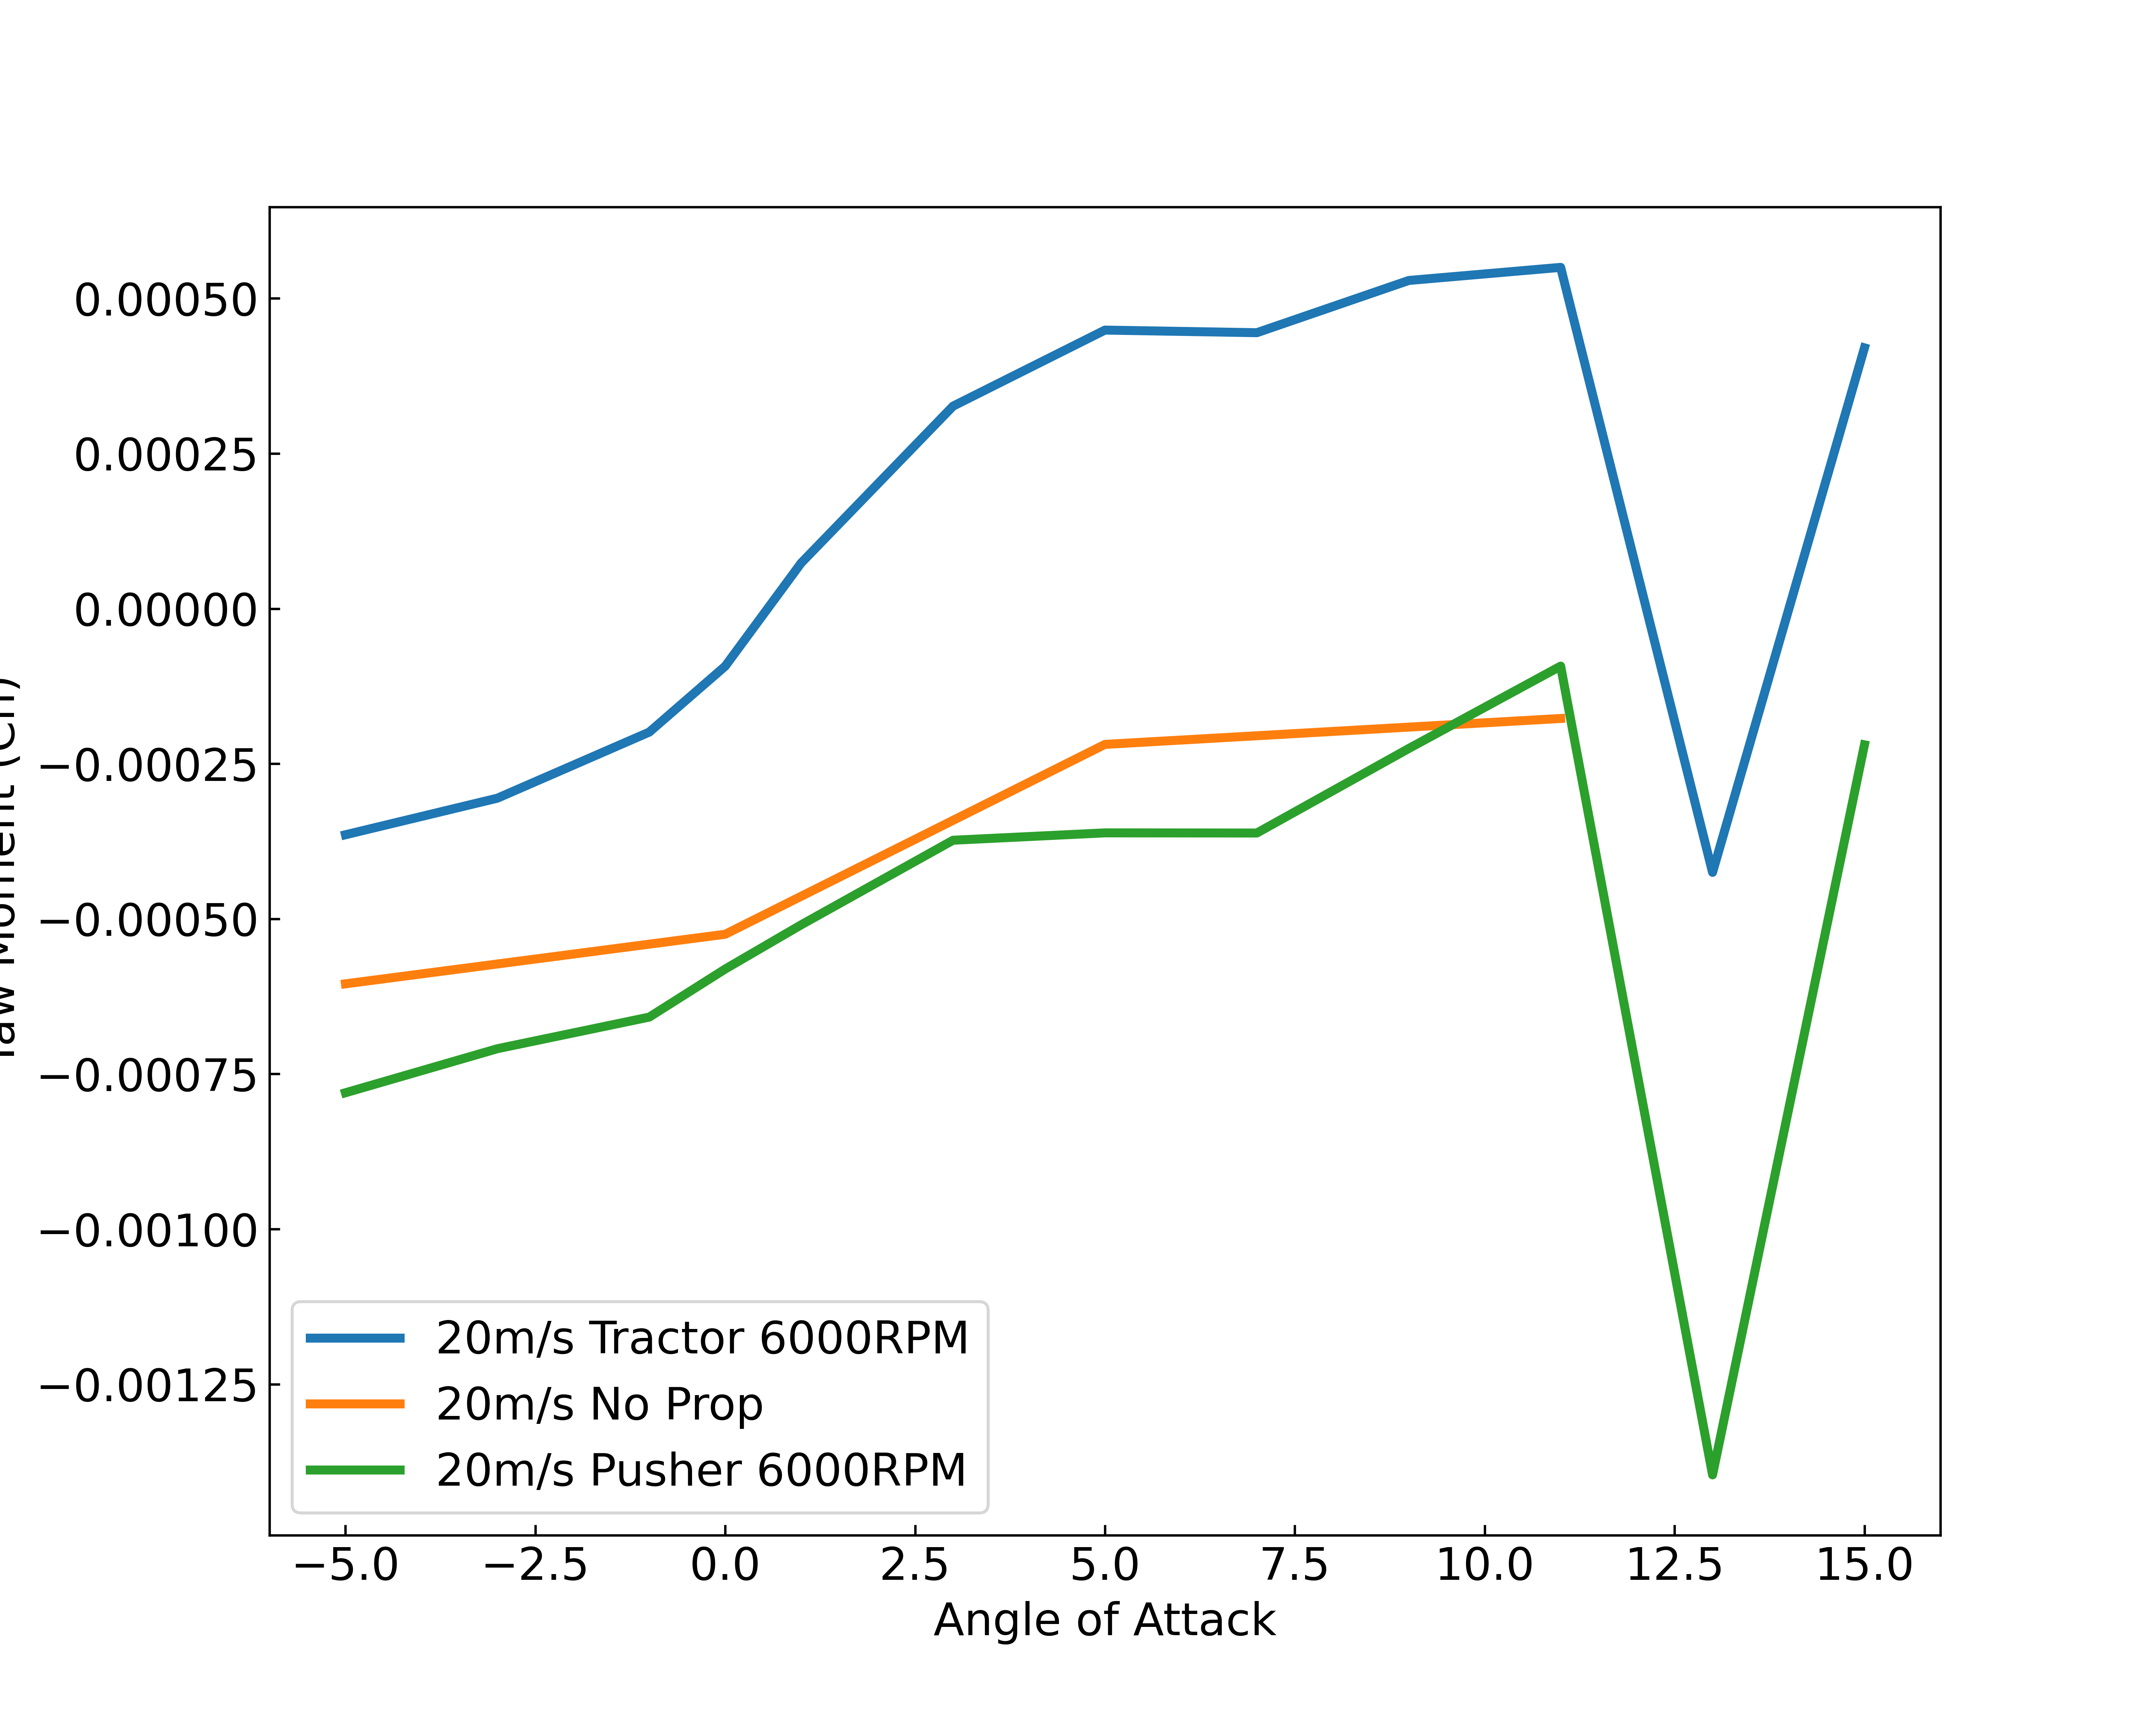
\includegraphics[width=\textwidth]{05_Results/Figs/Cn/20ms_6000RPM_Cn.png}
        \caption{Yawing Moment Coefficient at 20m/s airspeed and 6000RPM motor speed}
        \label{fig:Cn_20ms_6000}
    \end{subfigure}
    \begin{subfigure}[b]{0.467\textwidth}
        \centering
        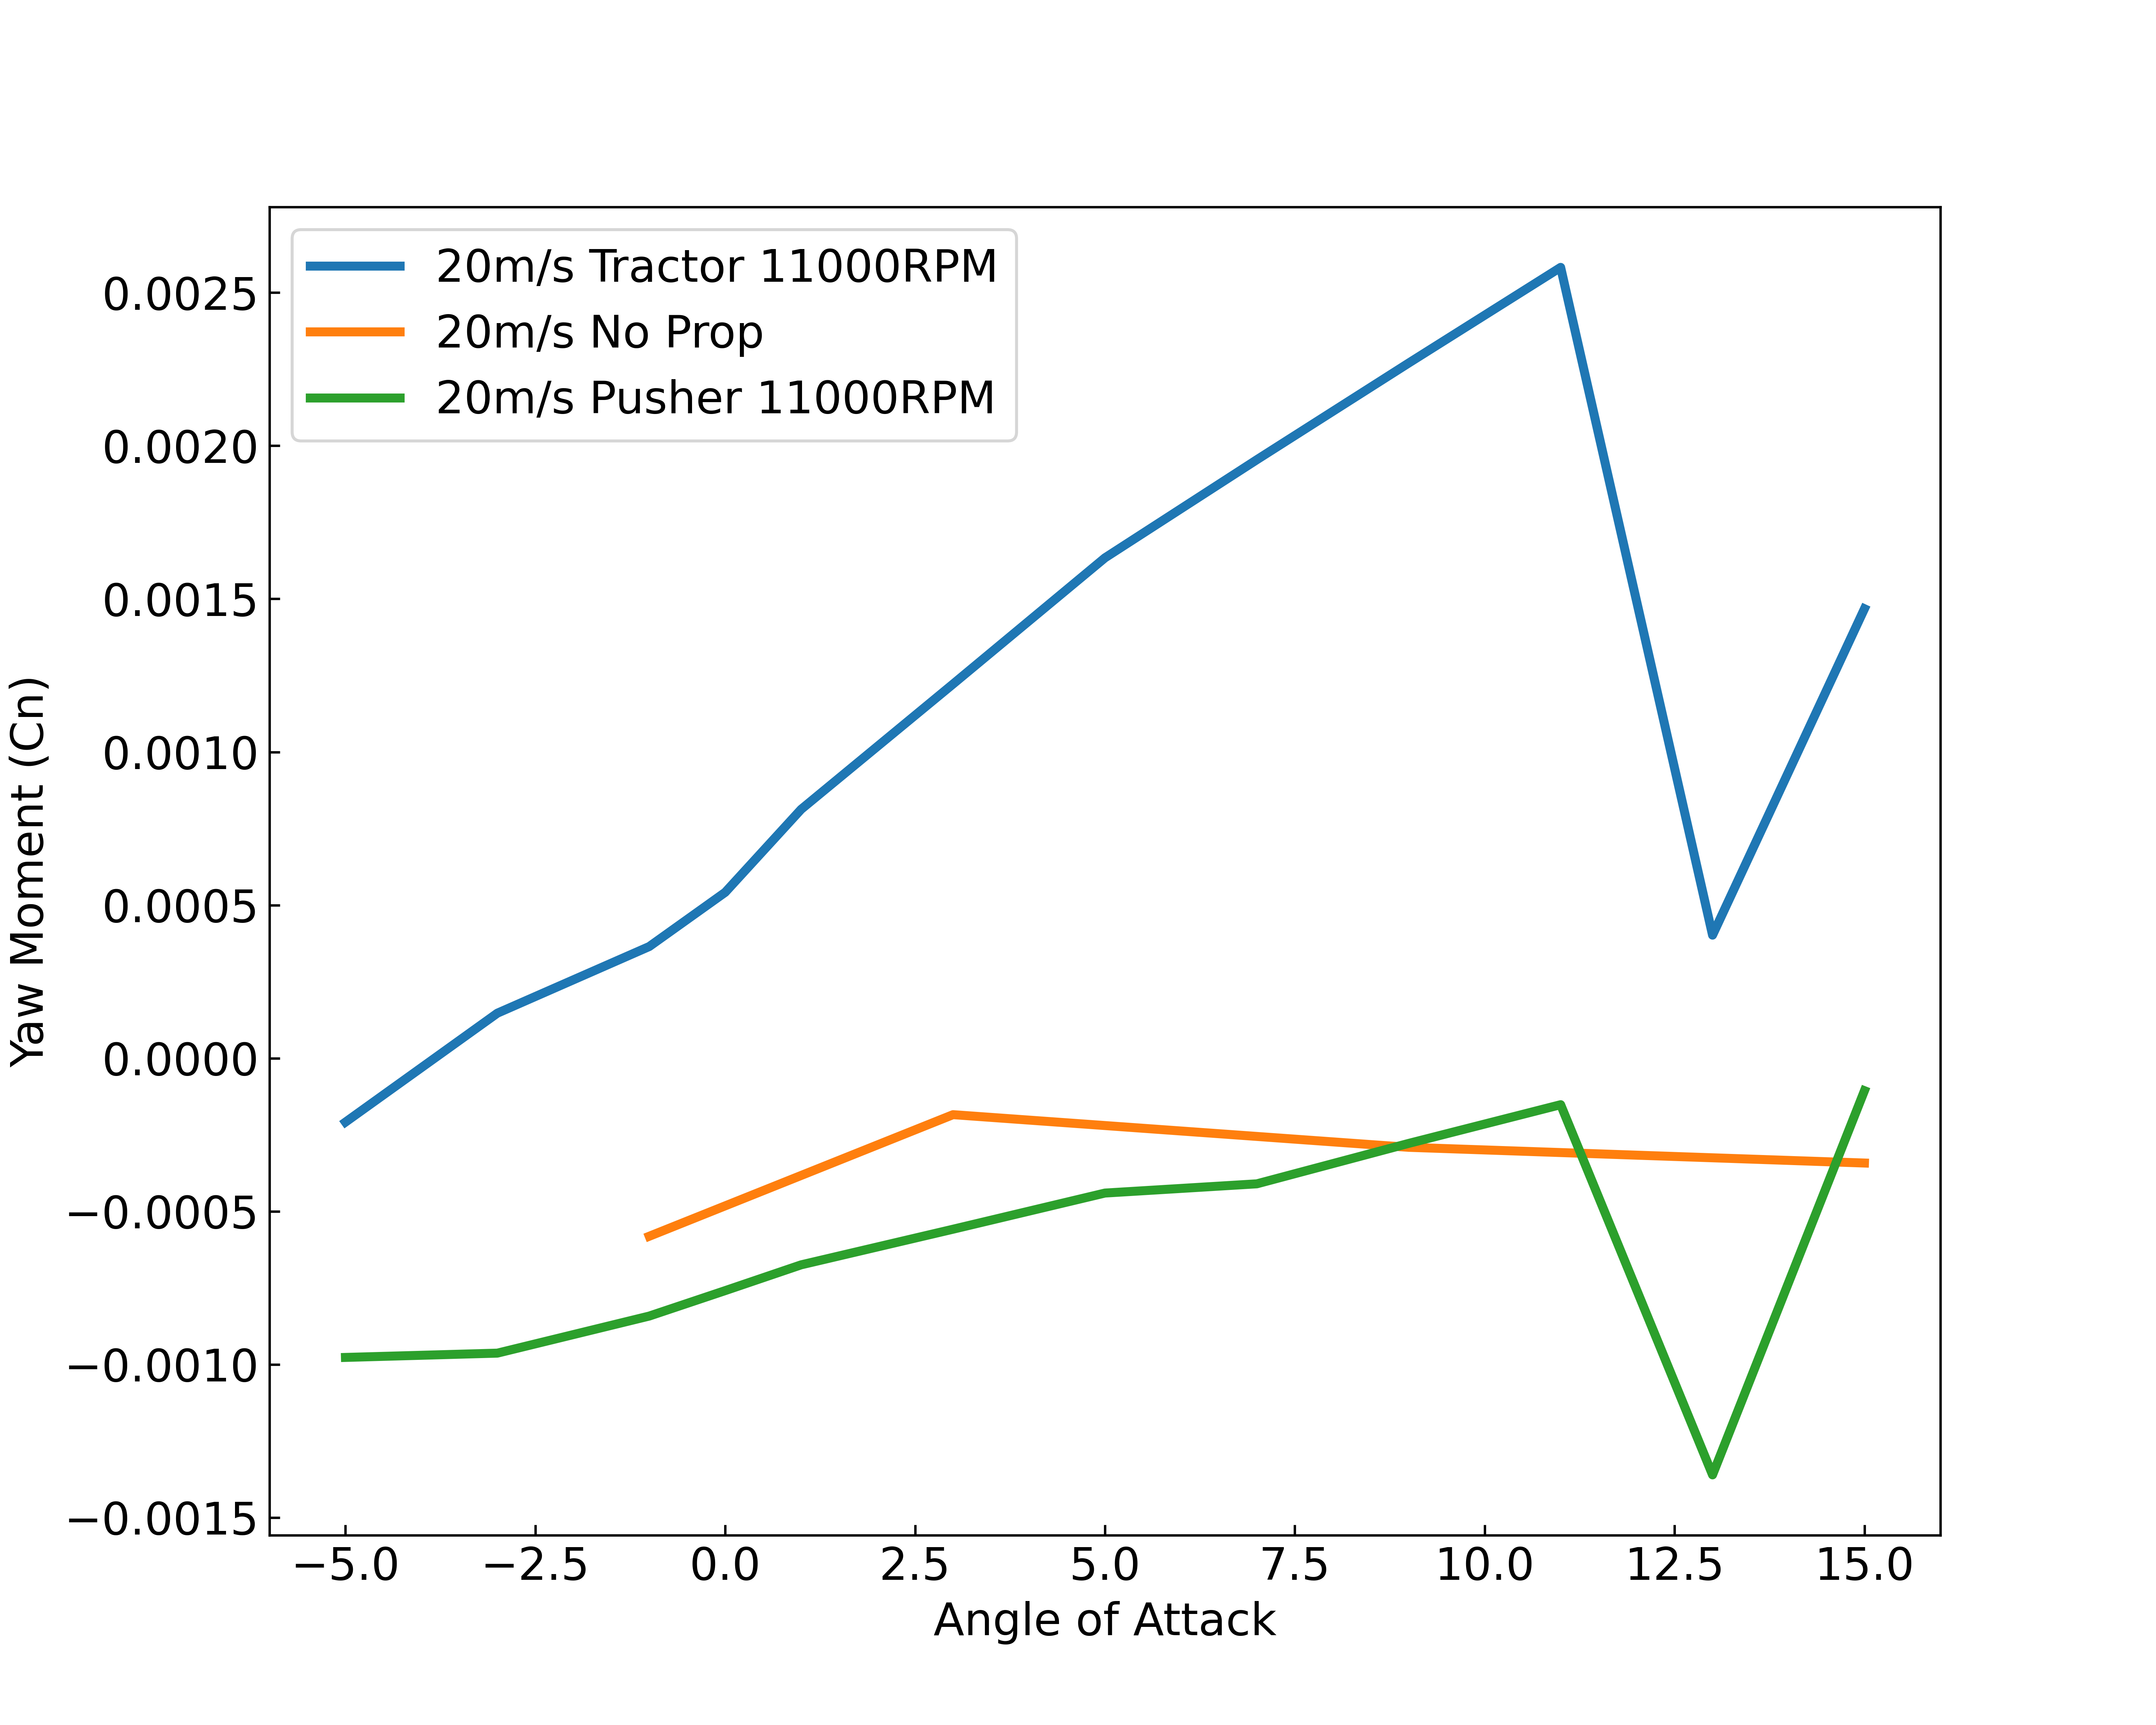
\includegraphics[width=\textwidth]{05_Results/Figs/Cn/20ms_11000RPM_Cn.png}
        \caption{Yawing Moment Coefficient at 20m/s airspeed and 11000RPM motor speed}
        \label{fig:Cn_20ms_11000}
    \end{subfigure}
\end{figure}




\subsection{Static Margin}
Figures \ref{fig:CmCl_10ms_6000} to \ref{fig:CmCl_20ms_11000} shows that the static margin for all configurations, airspeeds and propeller speeds tested was stable. The tractor configuration decreased the stability of the MAV except for the 10m$s^{-1}$ at 6000RPM propeller speed. This is also seen more clearly in Table \ref{tab:staticMargin} as static margin decreases from -0.155 to -0.107 when comparing the no propeller and tractor configurations at 11000RPM and  10m$s^{-1}$. At 6000RPM propeller speed, the tractor configuration became less stable when airspeed increased from 10m$s^{-1}$ to 20m$s^{-1}$, with the static margin decreasing from -0.116 to -0.106. This same trend was also seen for the pusher configuration at 6000RPM propeller speed, decreasing from -0.117 to -0.108. The opposite trend was seen when the propeller speed was increased to 11000RPM. The tractor and pusher configurations became more stable, increasing from -0.107 to -0.118 and from -0.156 to -0.173, respectively, when airspeed increased from 10m$s^{-1}$ to 20m$s^{-1}$. The no propeller configuration became more stable at all propeller speeds as the airspeed increased from 10m$s^{-1}$ to 20m$s^{-1}$.

\begin{table}
\caption{Static margin of all three configurations tested at airspeeds of 10m$s^{-1}$ and 20m$s^{-1}$, and propeller speeds of 6000RPM and 11000RPM}
\begin{tabular}{ |c|c|c|c| }

 \hline
 Configuration & Airspeed (ms$^{-1}$ &  Propeller Speed (\acrshort{RPM}) & Static Margin\\
 \hline
 Tractor & 10 & 6000 & -0.116 \\
 Tractor & 20 & 6000 & -0.106\\
No Propeller & 10 & 6000 & -0.100\\
  No Propeller & 20 & 6000 & -0.107 \\
 Pusher & 10 & 6000 & -0.117 \\
  Pusher & 20 & 6000 & -0.108 \\
  \hline
 Tractor & 10 & 11000 & -0.107 \\
 Tractor & 20 & 11000 & -0.118\\
 No Propeller & 10 & 11000 & -0.155\\
 No Propeller& 20 & 11000 & -0.159\\
 Pusher & 10 & 11000 & -0.156 \\
 Pusher & 20 & 11000 & -0.173 \\
 \hline
 

\end{tabular}
 \label{tab:staticMargin}
\end{table}
 


\begin{figure}[H]
    \centering
    \begin{subfigure}[b]{0.467\textwidth}
        \centering
        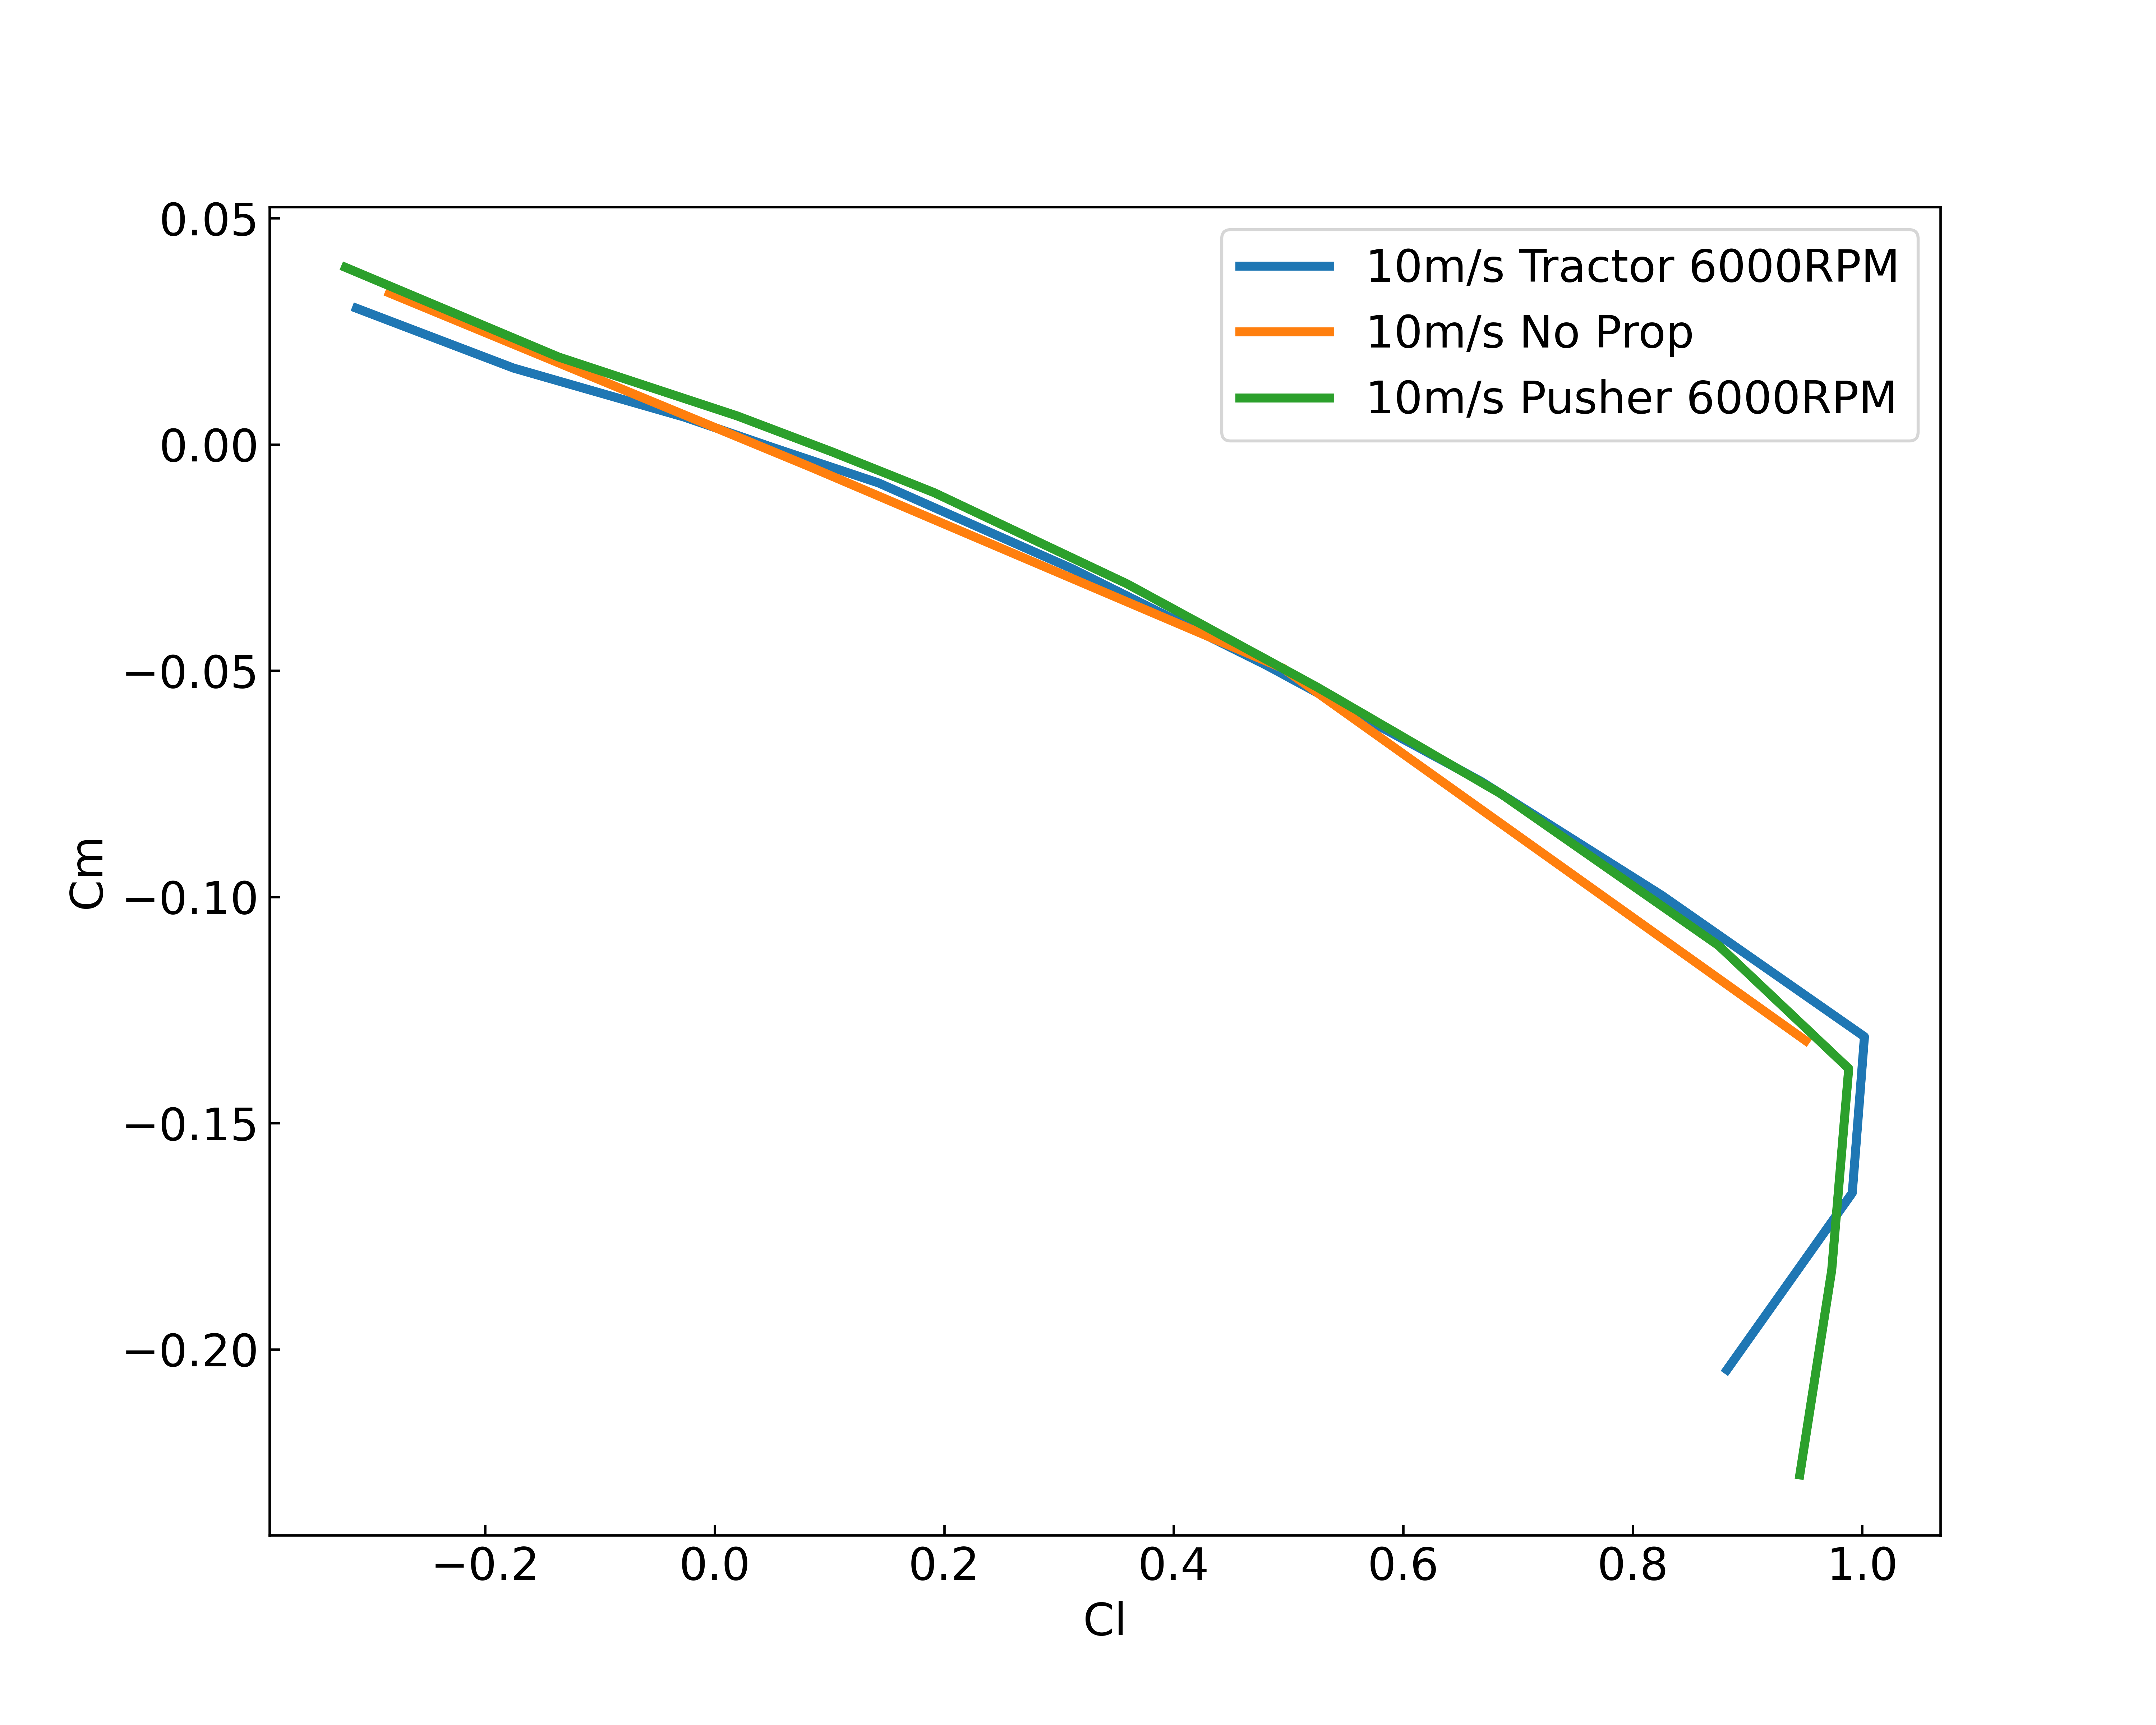
\includegraphics[width=\textwidth]{05_Results/Figs/ClCm/10ms_6000RPM_CmCl.png}
        \caption{Rolling Moment Coefficient at 10m/s airspeed and 6000RPM motor speed}
        \label{fig:CmCl_10ms_6000}
    \end{subfigure}
    \begin{subfigure}[b]{0.467\textwidth}
        \centering
        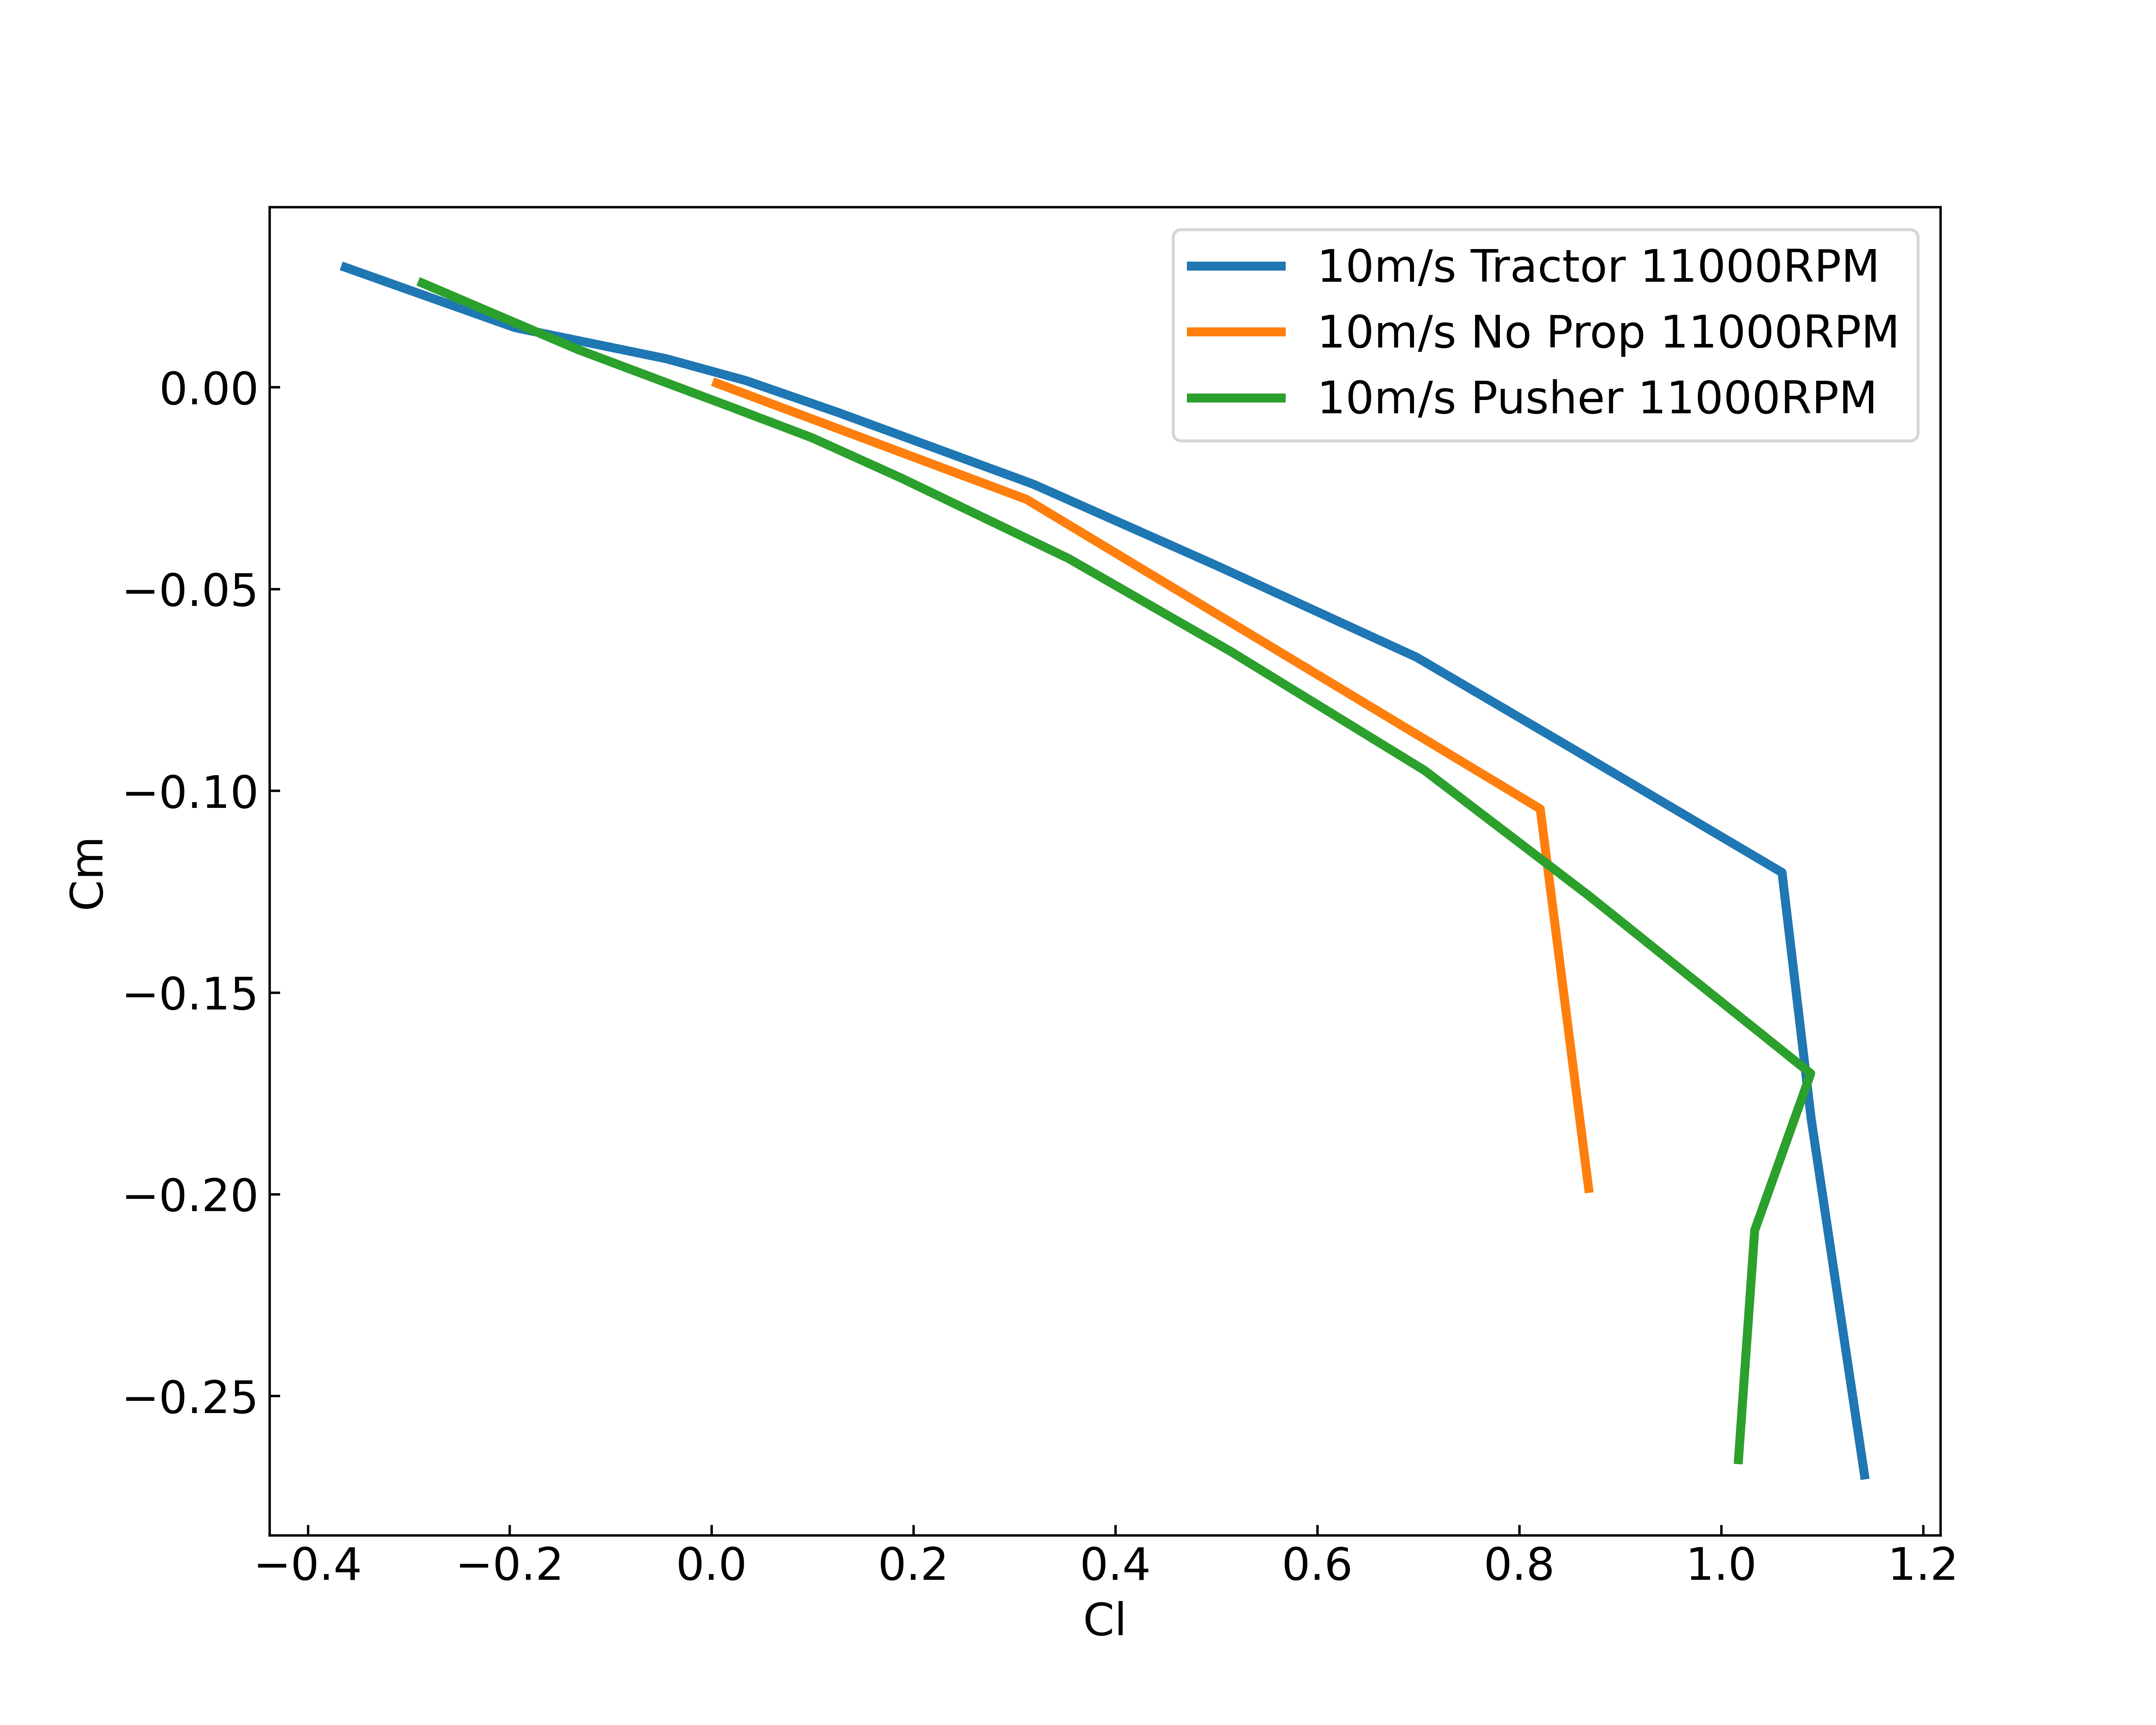
\includegraphics[width=\textwidth]{05_Results/Figs/ClCm/10ms_11000RPM_CmCl.png}
        \caption{Rolling Moment Coefficient at 10m/s airspeed and 11000RPM motor speed}
        \label{fig:CmCl_10ms_11000}
    \end{subfigure}
    \begin{subfigure}[b]{0.467\textwidth}
        \centering
        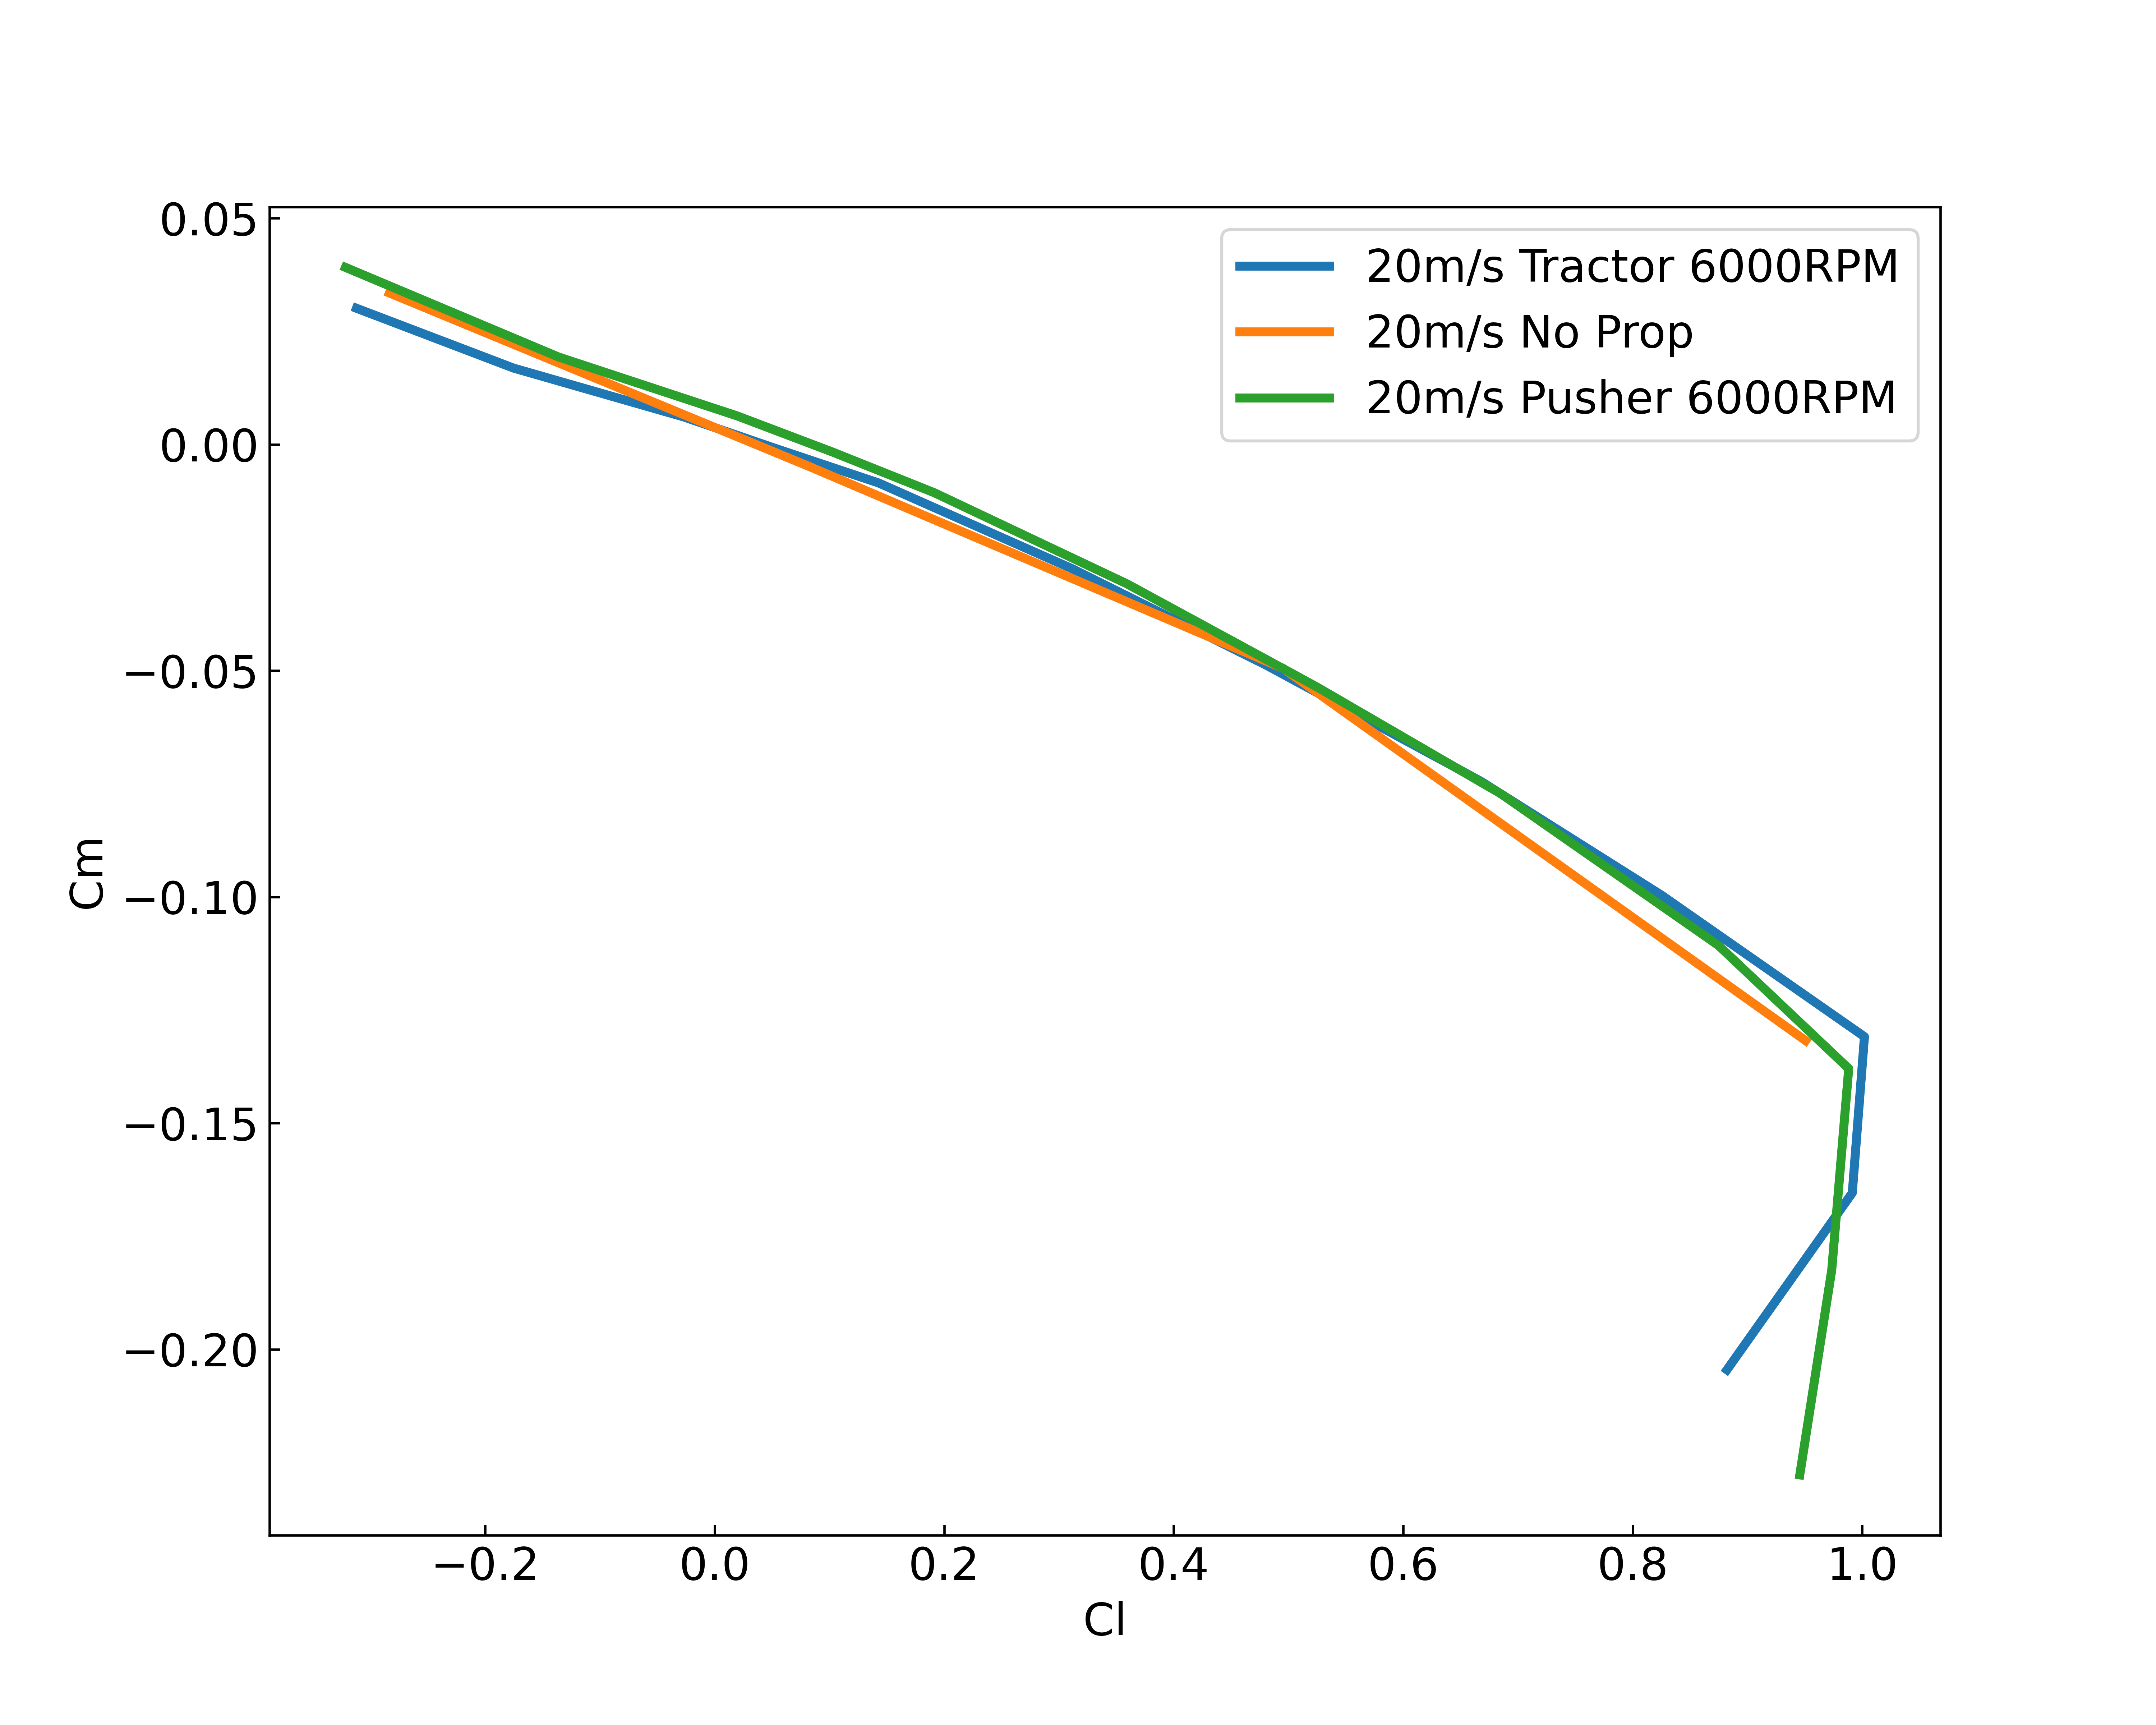
\includegraphics[width=\textwidth]{05_Results/Figs/ClCm/20ms_6000RPM_CmCl.png}
        \caption{Rolling Moment Coefficient at 20m/s airspeed and 6000RPM motor speed}
        \label{fig:CmCl_20ms_6000}
    \end{subfigure}
    \begin{subfigure}[b]{0.467\textwidth}
        \centering
        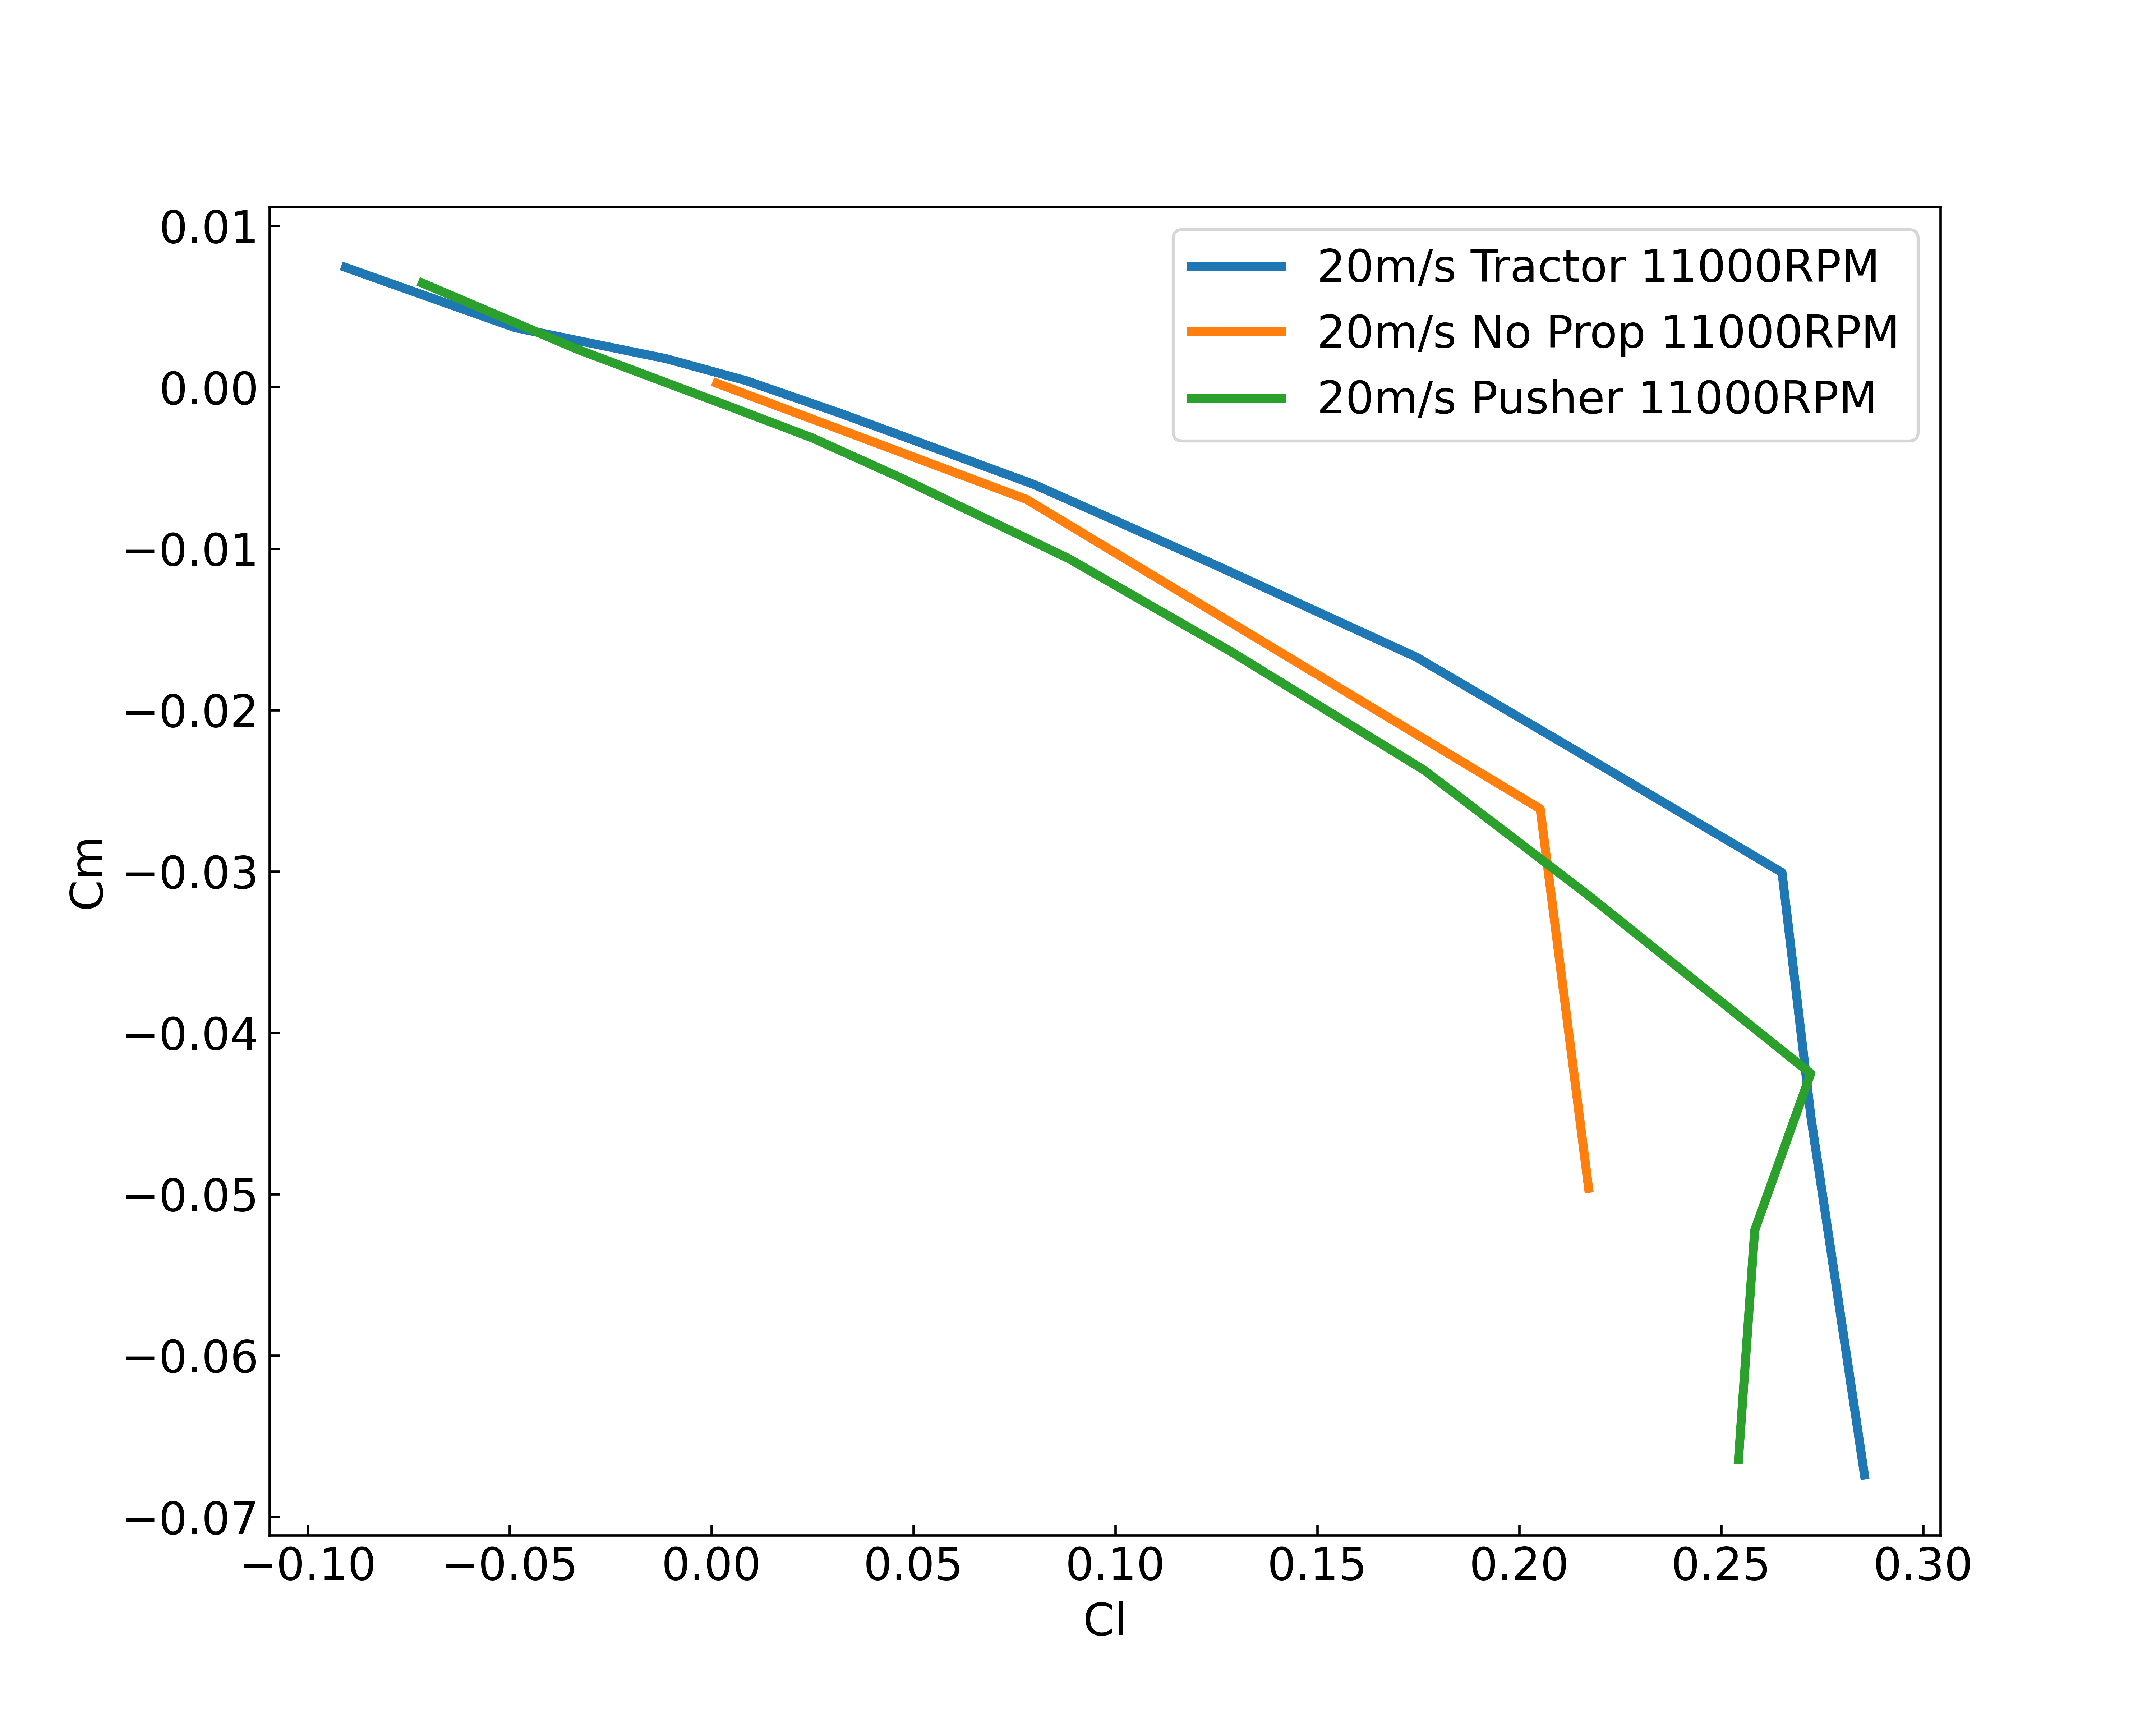
\includegraphics[width=\textwidth]{05_Results/Figs/ClCm/20ms_11000RPM_CmCl.png}
        \caption{Rolling Moment Coefficient at 20m/s airspeed and 11000RPM motor speed}
        \label{fig:CmCl_20ms_11000}
    \end{subfigure}
\end{figure}


\section{VAP 3.5 Validation}
Low-speed aerodynamics are described by complex flow distributions and phenomena as discussed in Sections \ref{sec:Reynolds} and \ref{sec:Reynolds2}. To evaluate the use of VAP 3.5 for the wind tunnel tests conducted, a wing validation and model validation was performed with comparison to the \acrshort{GenMAV} model, which has been previously evaluated with the Athena Vortex Lattice (\acrshort{AVL}) method to estimate the stability derivatives and moments of the \acrshort{GenMAV}. A rectangle wing shape was used in this analysis with the S5010, a root chord of 0.17m, \acrshort{AR} of 3 and three taper configurations which are 0.3, 0.5 and 1.


\subsection{Wing Validation}
 Figures \ref{fig:wing0300} to Figure \ref{fig:001000b} show a wing validation against Fluent \acrshort{CFD} results \cite{Trips}. This data was taken at a Reynolds number of 2.32 $\times 10^{5}$ at a freestream velocity of 20$m/s$ and density 1.225$kg/m^3$. Figures \ref{fig:wing0300} to \ref{fig:001000b} showed strong agreement with the \acrshort{CFD} results for the coefficient of lift and L/D ratios for the three tapered wings. 

\begin{figure}[H]
     \centering
     \begin{subfigure}[b]{0.45\textwidth}
         \centering
         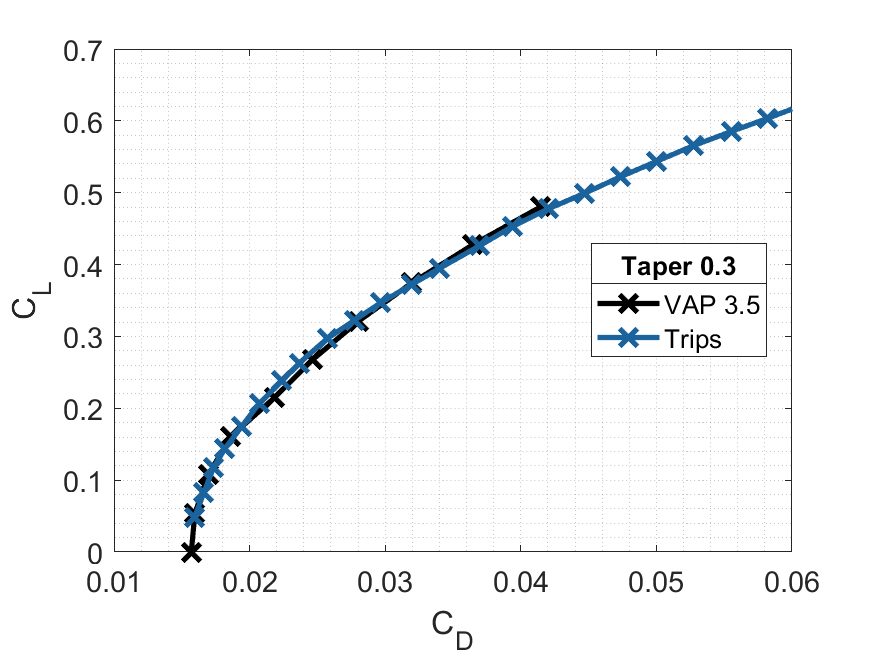
\includegraphics[width=\textwidth]{05_Results/Figs/VAP/genMAV/taper3a.png}
         \caption{}
         \label{fig:wing0300}

     \end{subfigure}
     \hfill
     \begin{subfigure}[b]{0.45\textwidth}
         \centering
         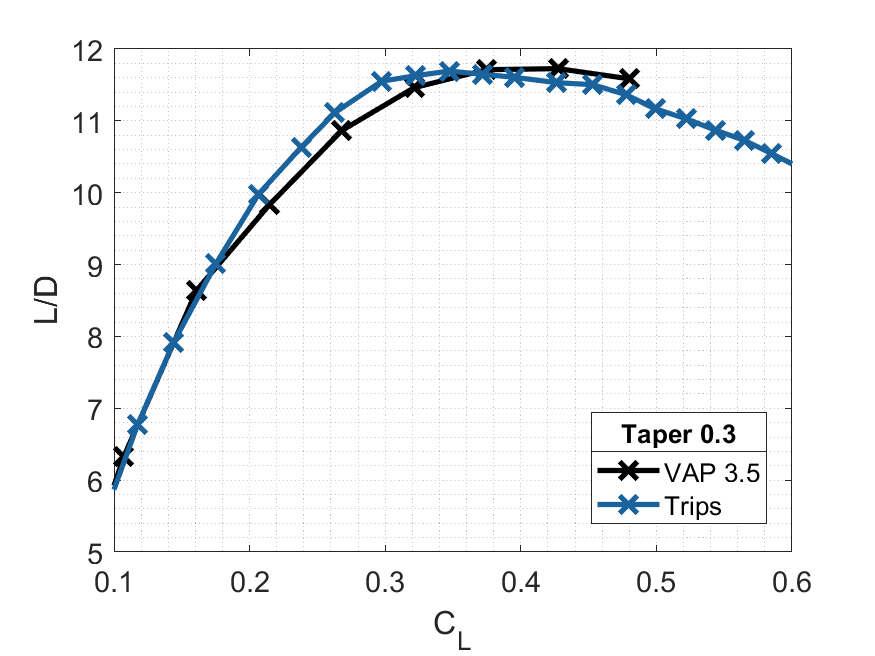
\includegraphics[width=\textwidth]{05_Results/Figs/VAP/genMAV/taper3b.png}
         \caption{}
         \label{fig:wing0300b}
      
     \end{subfigure}
     \hfill

        
\end{figure}


\begin{figure}[H]
     \centering
     \begin{subfigure}[b]{0.45\textwidth}
         \centering
         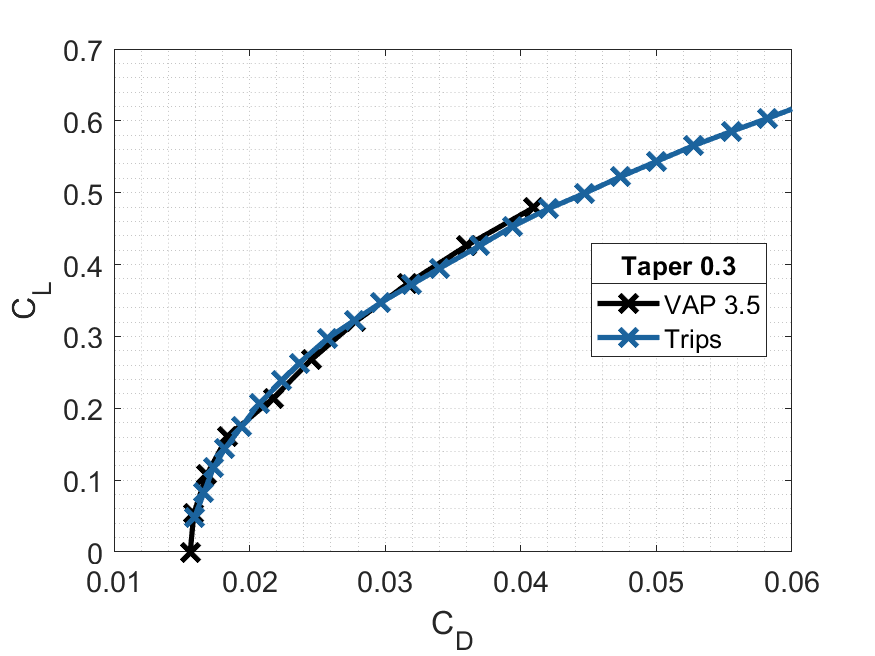
\includegraphics[width=\textwidth]{05_Results/Figs/VAP/genMAV/taper5a.png}
        \label{fig:morelabel}
     \end{subfigure}
     \hfill
     \begin{subfigure}[b]{0.45\textwidth}
         \centering
         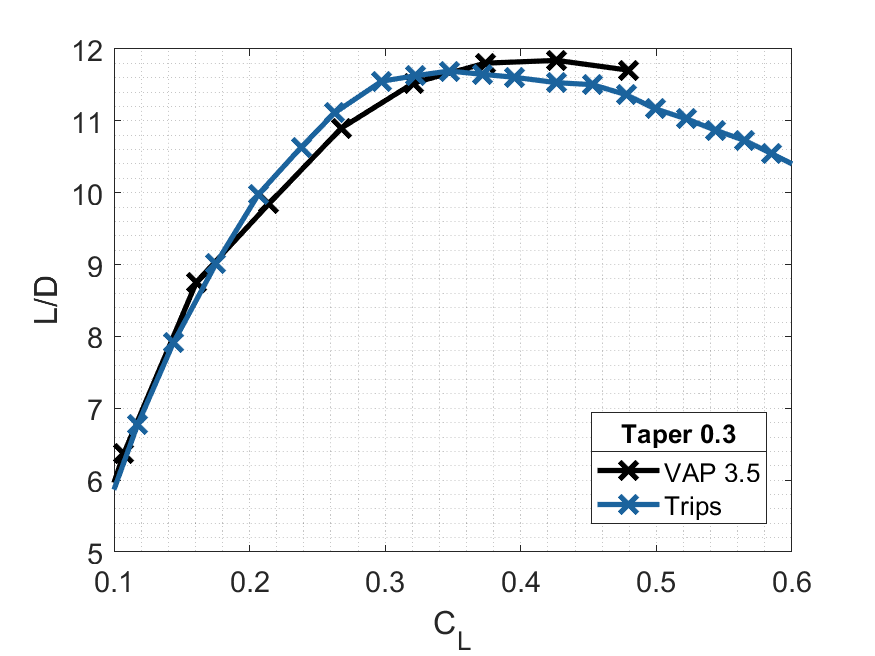
\includegraphics[width=\textwidth]{05_Results/Figs/VAP/genMAV/taper5b.png}
         \label{fig:forlabel}
      
     \end{subfigure}
     \hfill

        
\end{figure}


\begin{figure}[H]
     \centering
     \begin{subfigure}[b]{0.45\textwidth}
         \centering
         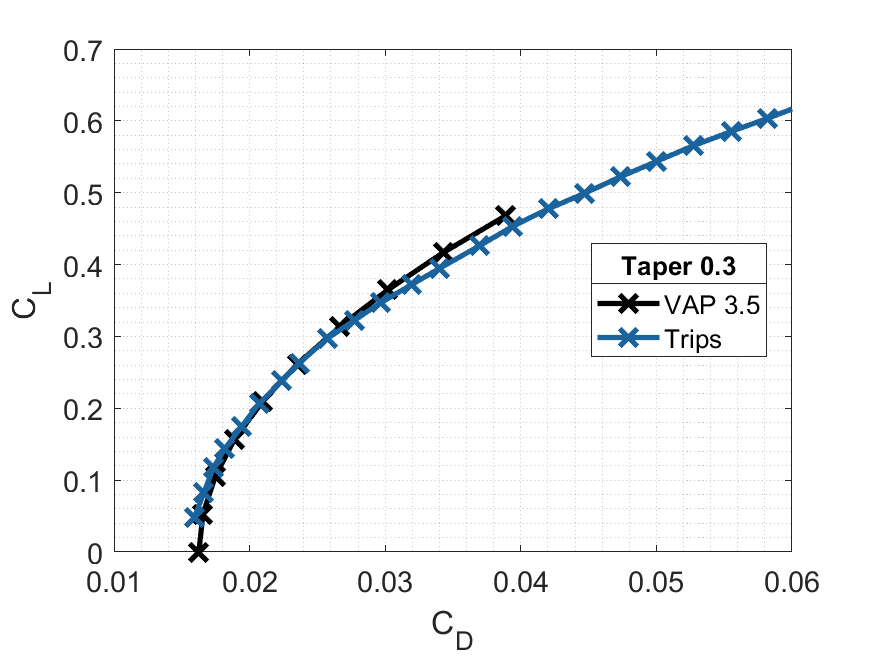
\includegraphics[width=\textwidth]{05_Results/Figs/VAP/genMAV/taper10a.png}
         \label{fig:thinkin2}

     \end{subfigure}
     \hfill
     \begin{subfigure}[b]{0.45\textwidth}
         \centering
         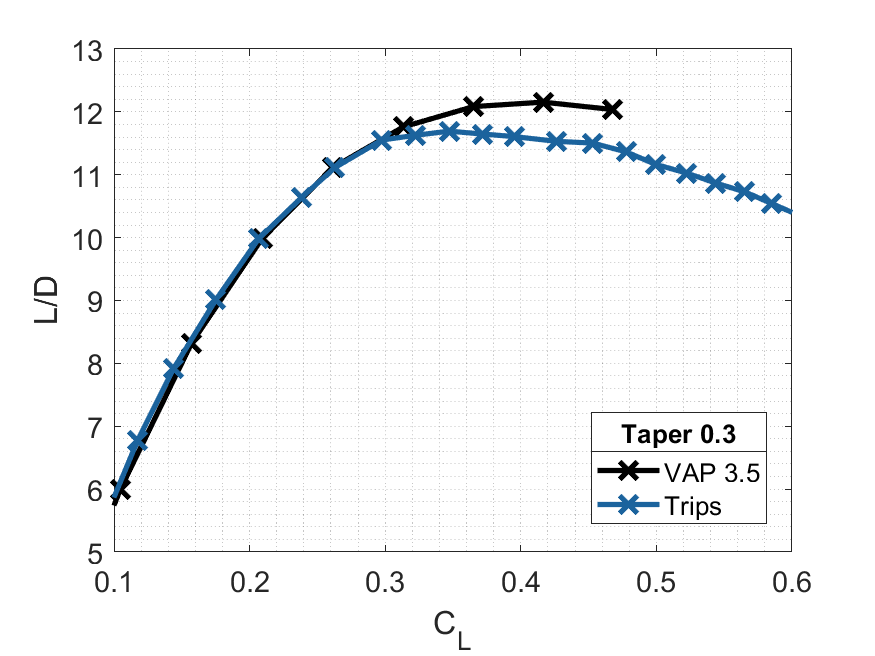
\includegraphics[width=\textwidth]{05_Results/Figs/VAP/genMAV/taper10b.png}
         \caption{}
         
      \label{fig:001000b}
     \end{subfigure}
     \hfill

        
\end{figure}





\subsection{\acrshort{GenMAV} model validation}
A model validation was also conducted in order to assess how accurate the stability coefficient calculations were for a non-propelled \acrshort{MAV}. A validation against a propelled \acrshort{MAV} could not be completed due to a lack of data. The GenMAV is a baseline \acrshort{MAV} designed for further development and testing. Due to this it features many typical \acrshort{MAV} aspects for its configuration. It features a conventional wing and empennage with a thin cambered plate airfoil. The thin cambered plate was approximated with the Eppler E387 in order to best match the camber of the GenMAV airfoil. The stability coefficients shown in Figures \ref{fig:genMAV_Cm} to \ref{fig:genMAV_Cn} show reasonable agreement with the \acrshort{AVL} method \cite{Stewart2007}. The inaccurarcies seen below 0$^\circ$ \acrshort{AoA} in Figure \ref{fig:genMAV_Cm} for the pitching moment are due to the way in which VAP 3.5 calculates the forces acting on the model. Discrepancies are also seen in Figures \ref{fig:genMAV_Cl_roll} and \ref{fig:genMAV_Cn}, however to a lesser extent. These discrepancies are more likely due to the geometry used to model the GenMAV not being exactly the same as features such as the curve of a fuselage profile are not implemented in current software \cite{Stewart2007}.

\begin{figure}[H]
     \centering
     \begin{subfigure}[b]{0.45\textwidth}
          \centering
        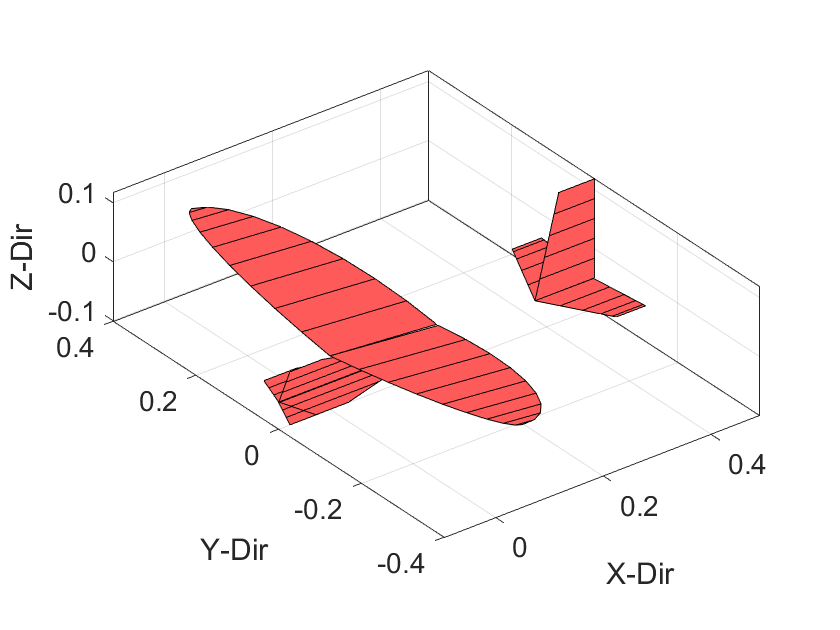
\includegraphics[width=\textwidth]{05_Results/Figs/VAP/genMAV/modelb.png}
        \caption{VAP 3.5 model of GenMAV}
            \label{fig:genMAVDimensions}
            

     \end{subfigure}
     \begin{subfigure}[b]{0.45\textwidth}
                \centering
            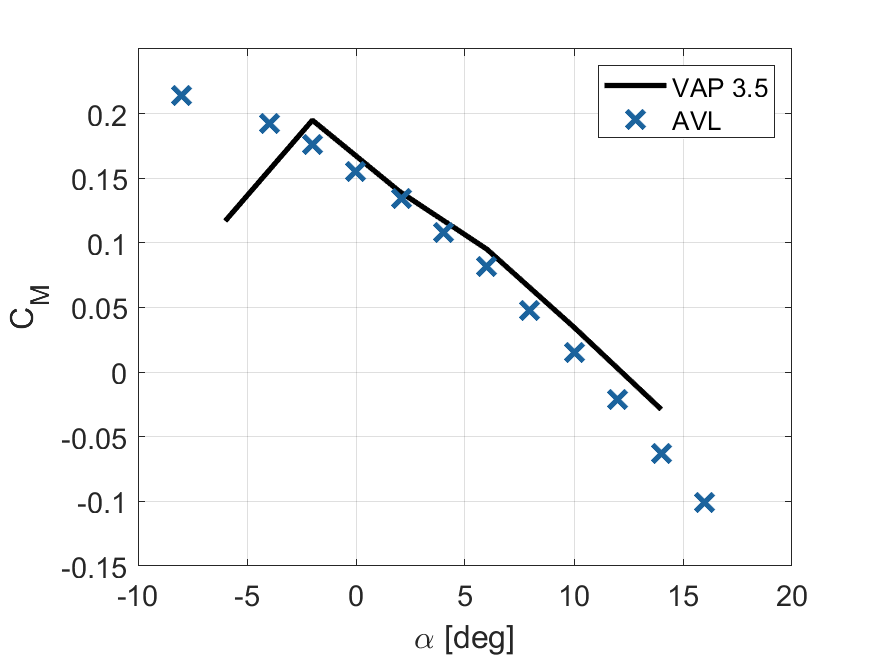
\includegraphics[width=\textwidth]{05_Results/Figs/VAP/genMAV/GenMAVModelValidation1.png}
            
              \caption{Pitching moment comparison for GenMAV between VAP 3.5 and AVL \cite{Stewart2007}}
               \label{fig:genMAV_Cm}
     \end{subfigure}
     \begin{subfigure}[b]{0.45\textwidth}
            \centering
         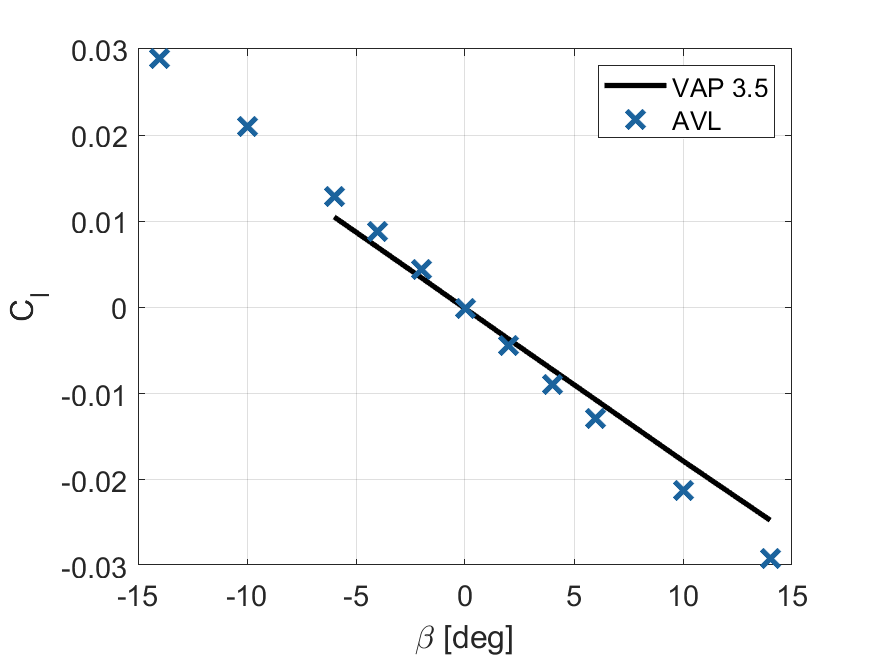
\includegraphics[width=\textwidth]{05_Results/Figs/VAP/genMAV/GenMAVModelValidation2.png}
        
         \caption{Rolling moment comparison for GenMAV between VAP 3.5 and AVL \cite{Stewart2007}}
          \label{fig:genMAV_Cl_roll}

     \end{subfigure}
     \begin{subfigure}[b]{0.45\textwidth}
               \centering
         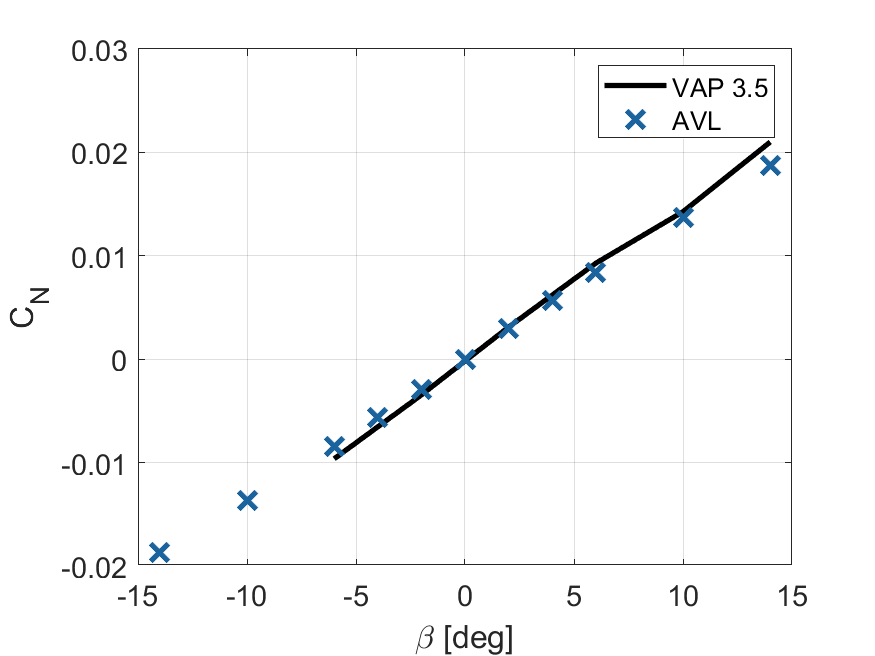
\includegraphics[width=\textwidth]{05_Results/Figs/VAP/genMAV/GenMAVModelValidation3.png}
         
         \caption{Yawing moment comparison for GenMAV between VAP 3.5 and AVL \cite{Stewart2007}}
         \label{fig:genMAV_Cn}
     \end{subfigure}
\end{figure}








\subsection{Validation of Wind Tunnel Results with VAP 3.5}

In order to determine the accuracy of the wind tunnel results obtained and assess VAP 3.5's ability to calculate the stability coefficients which define the MAV. A comparison has been made between the results seen in the wind tunnel and the results obtained when running VAP 3.5 for the developed model for the three configurations analysed.



\subsubsection{No Propeller Configuration}
 Figure \ref{fig:nopropmodelVAP} outlines a partially completed run. All no-propeller VAP 3.5 analyses were run until the wing wake and tail wake had fully developed to most accurately determine the stability coefficients acting on the model.
 \begin{figure}
 \centering
        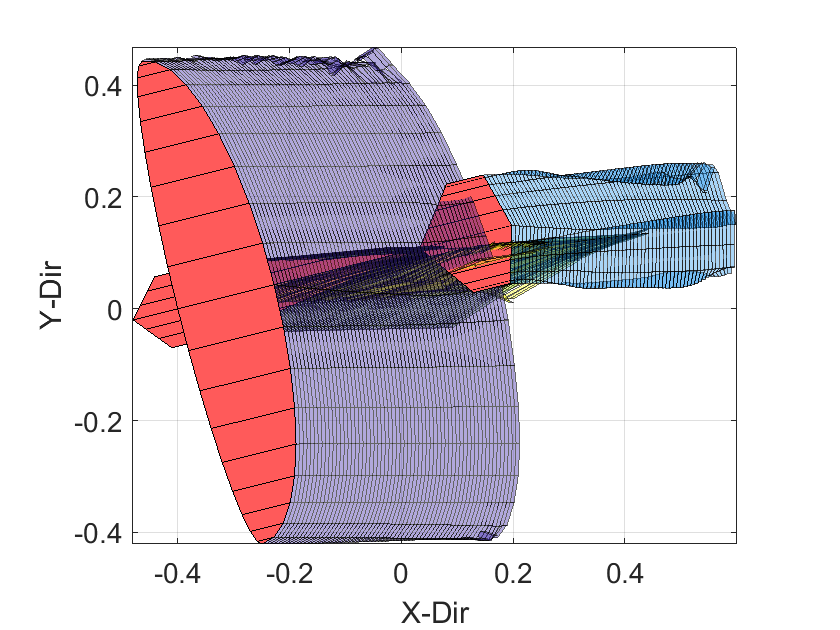
\includegraphics[width=0.5\textwidth]{05_Results/Figs/wake.png}
        \caption{No propeller configuration showing the start of the wake interference when run through VAP 3.5}
        \label{fig:nopropmodelVAP}
\end{figure}
 
Figures \ref{fig:VAP_noProp_Cm_10ms_6000} to \ref{fig:VAP_NoProp_Cl_20ms_11000} show that the rolling moment shows significant discrepancies for the no propeller configuration in all tested cases. The current side force and moments calculations are still being tested in VAP 3.5 and are currently highly dependent on the geometry defined. While the geometry of the \acrshort{MAV} model has been kept the same where possible, several features, such as the curve of the fuselage and wing, have been approximated with flat plates and approximate equations, respectively.


\begin{figure}[H]
    \centering
    \begin{subfigure}[b]{0.4\textwidth}
        \centering
        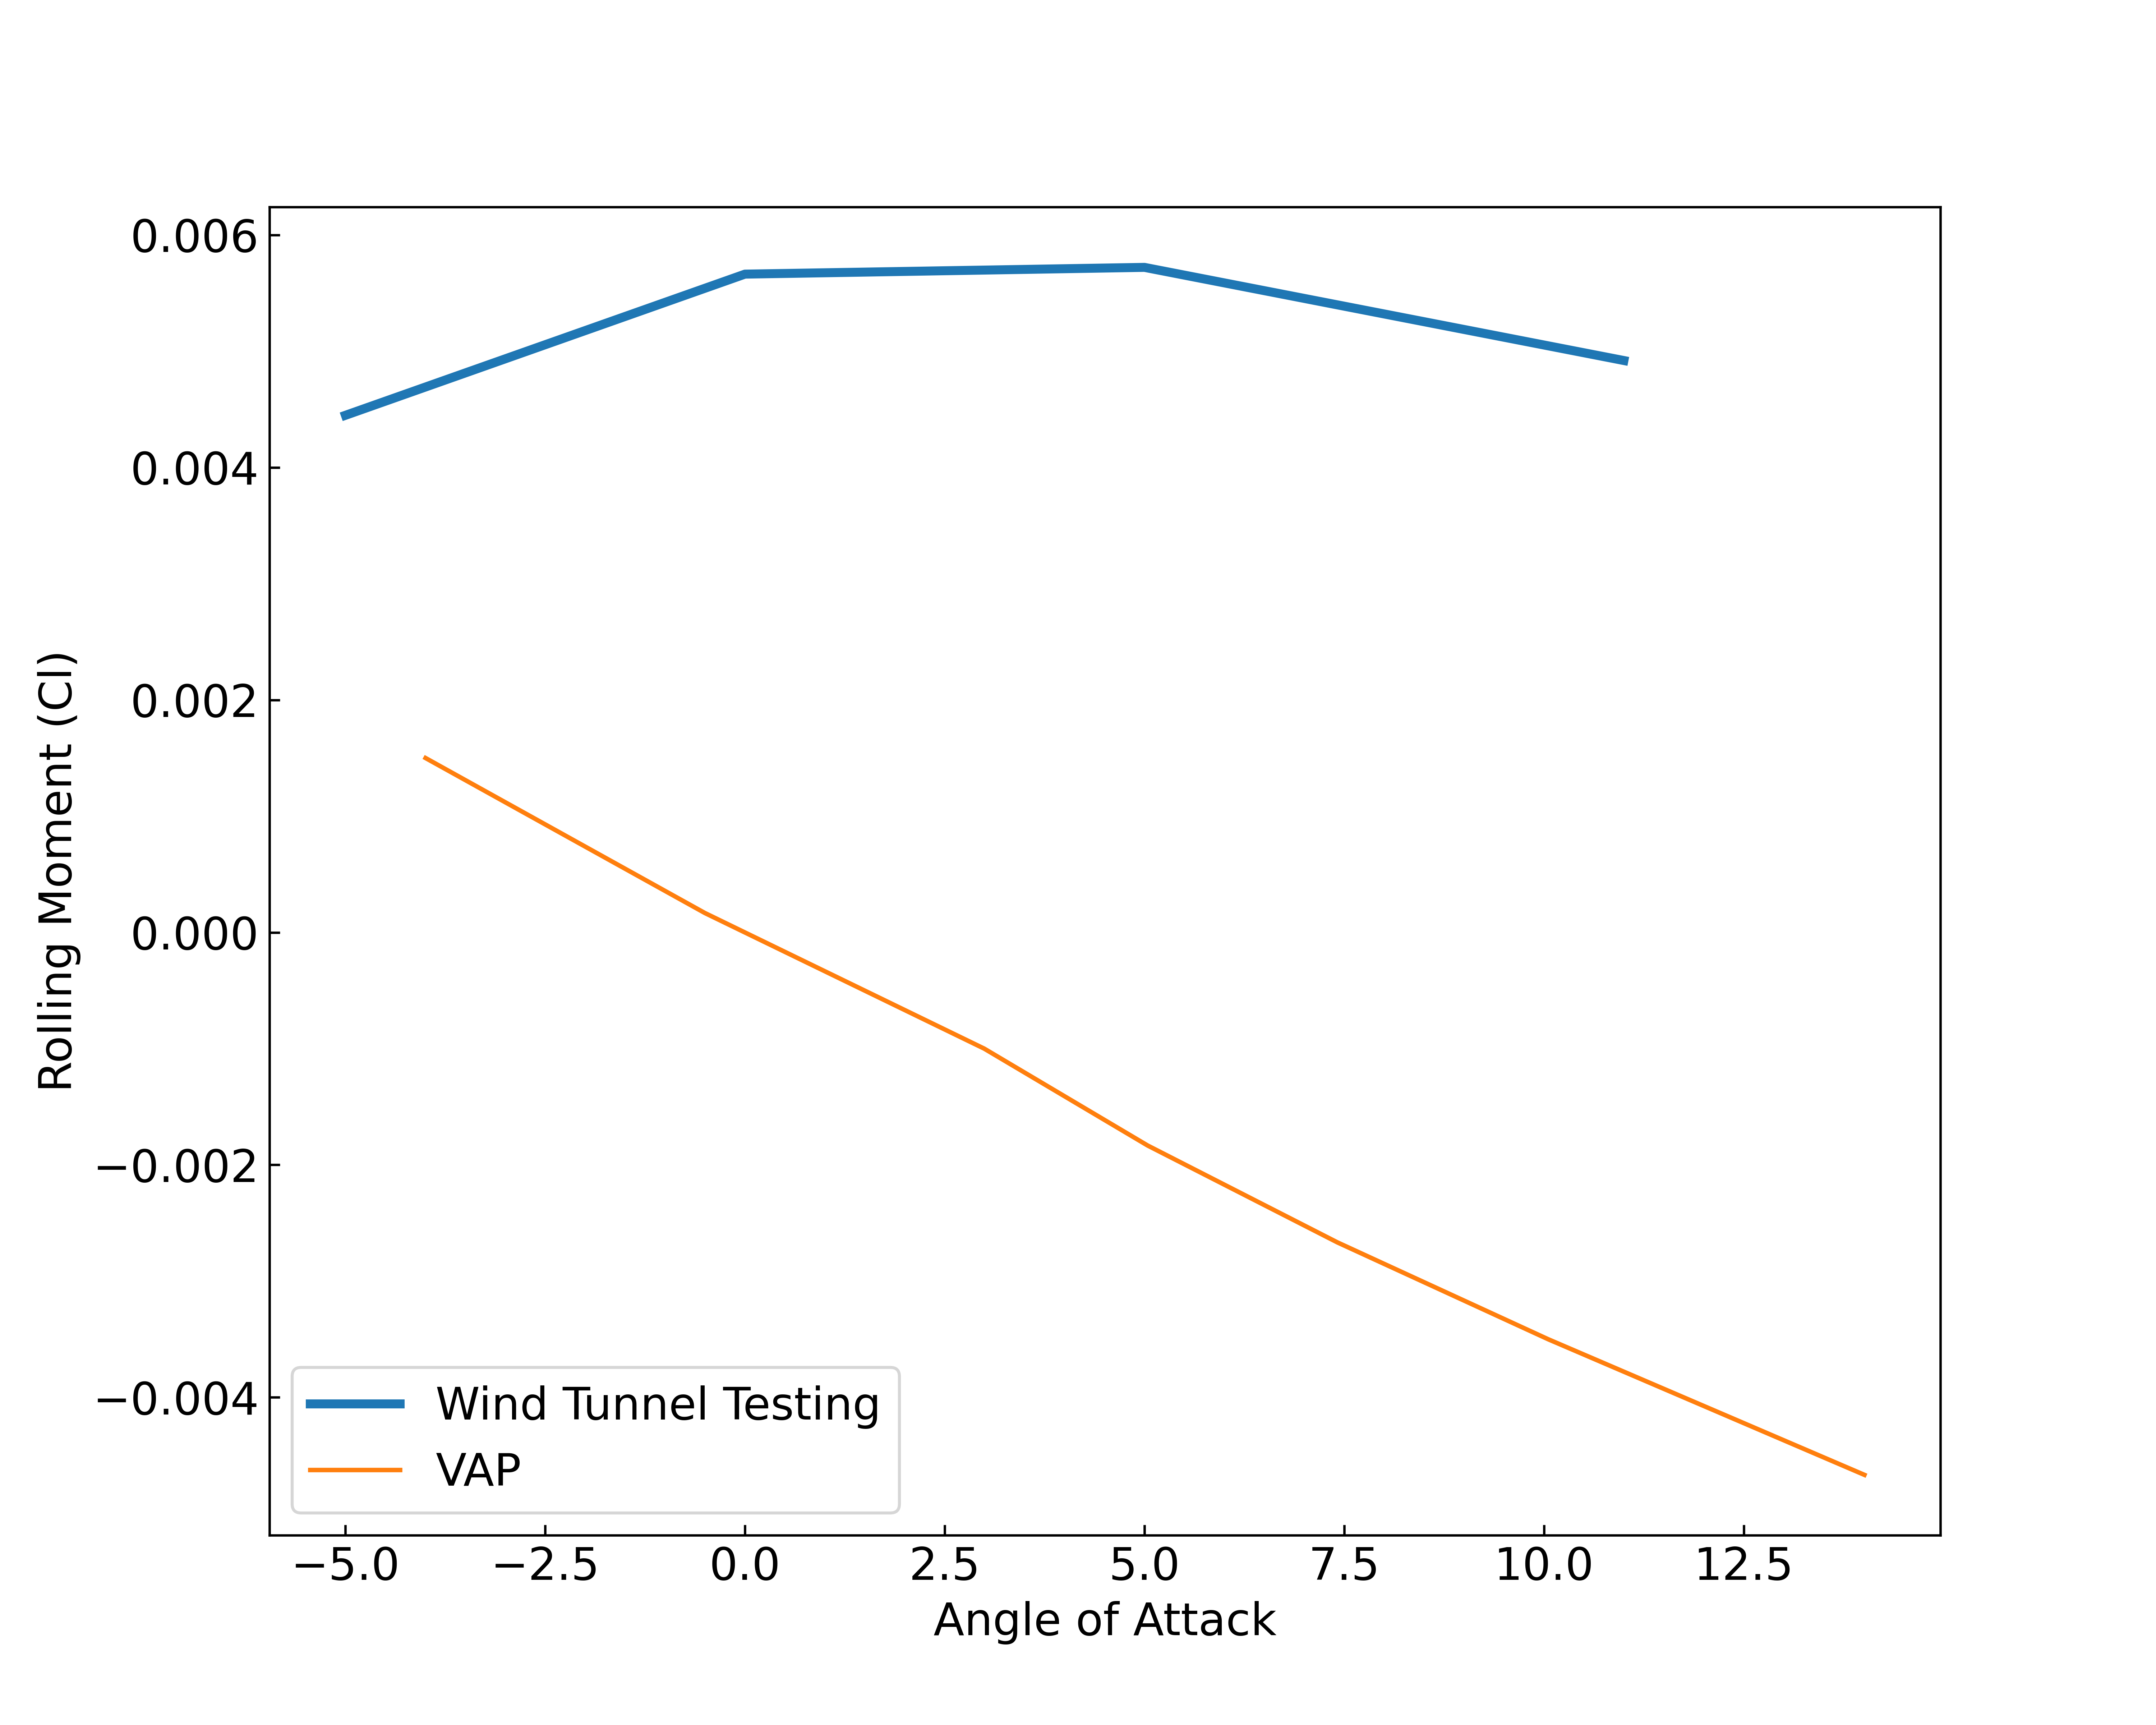
\includegraphics[width=\textwidth]{05_Results/VAP/noProp/Cl/10ms_6000RPM_Cl.png}
        \caption{Rolling Moment Coefficient at 10m/s airspeed for no propeller configuration}
        \label{fig:VAP_NoProp_Cl_10ms_6000}
    \end{subfigure}
    \begin{subfigure}[b]{0.46\textwidth}
        \centering
        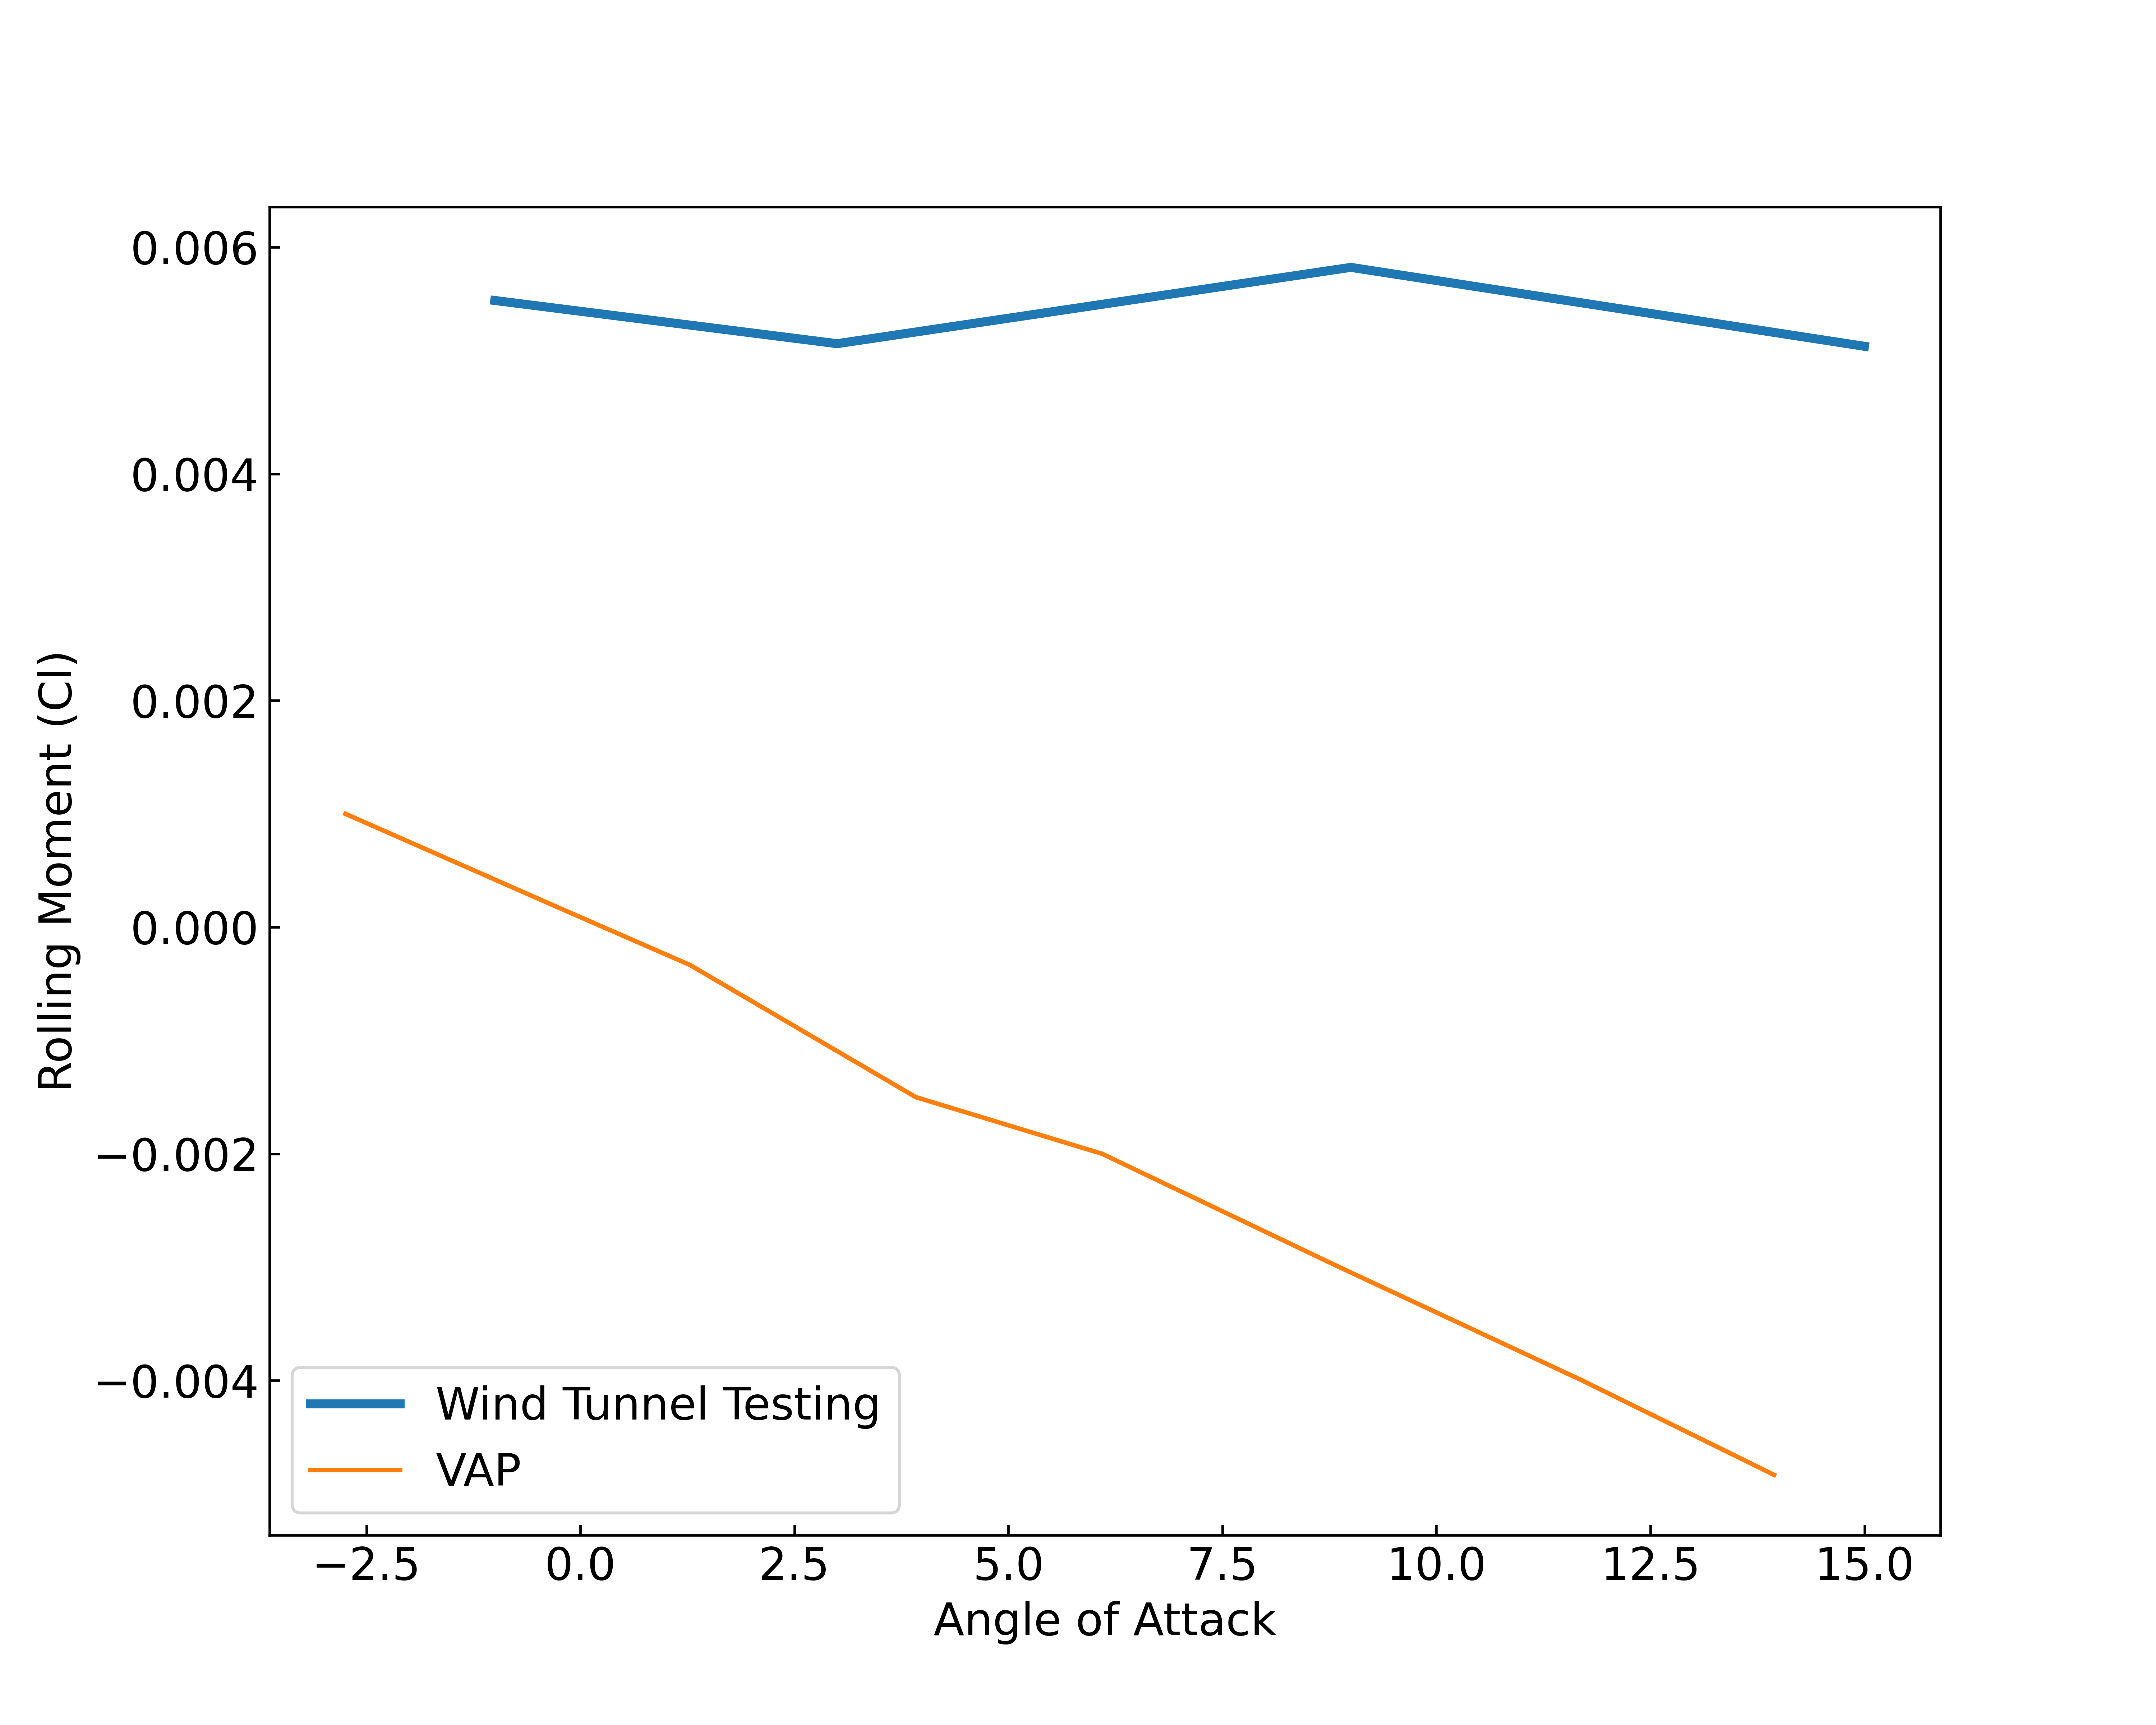
\includegraphics[width=\textwidth]{05_Results/VAP/noProp/Cl/10ms_11000RPM_Cl.png}
        \caption{Rolling Moment Coefficient at 10m/s airspeed for no propeller configuration}
        \label{fig:VAP_NoProp_Cl_10ms_11000}
    \end{subfigure}
    \begin{subfigure}[b]{0.467\textwidth}
        \centering
        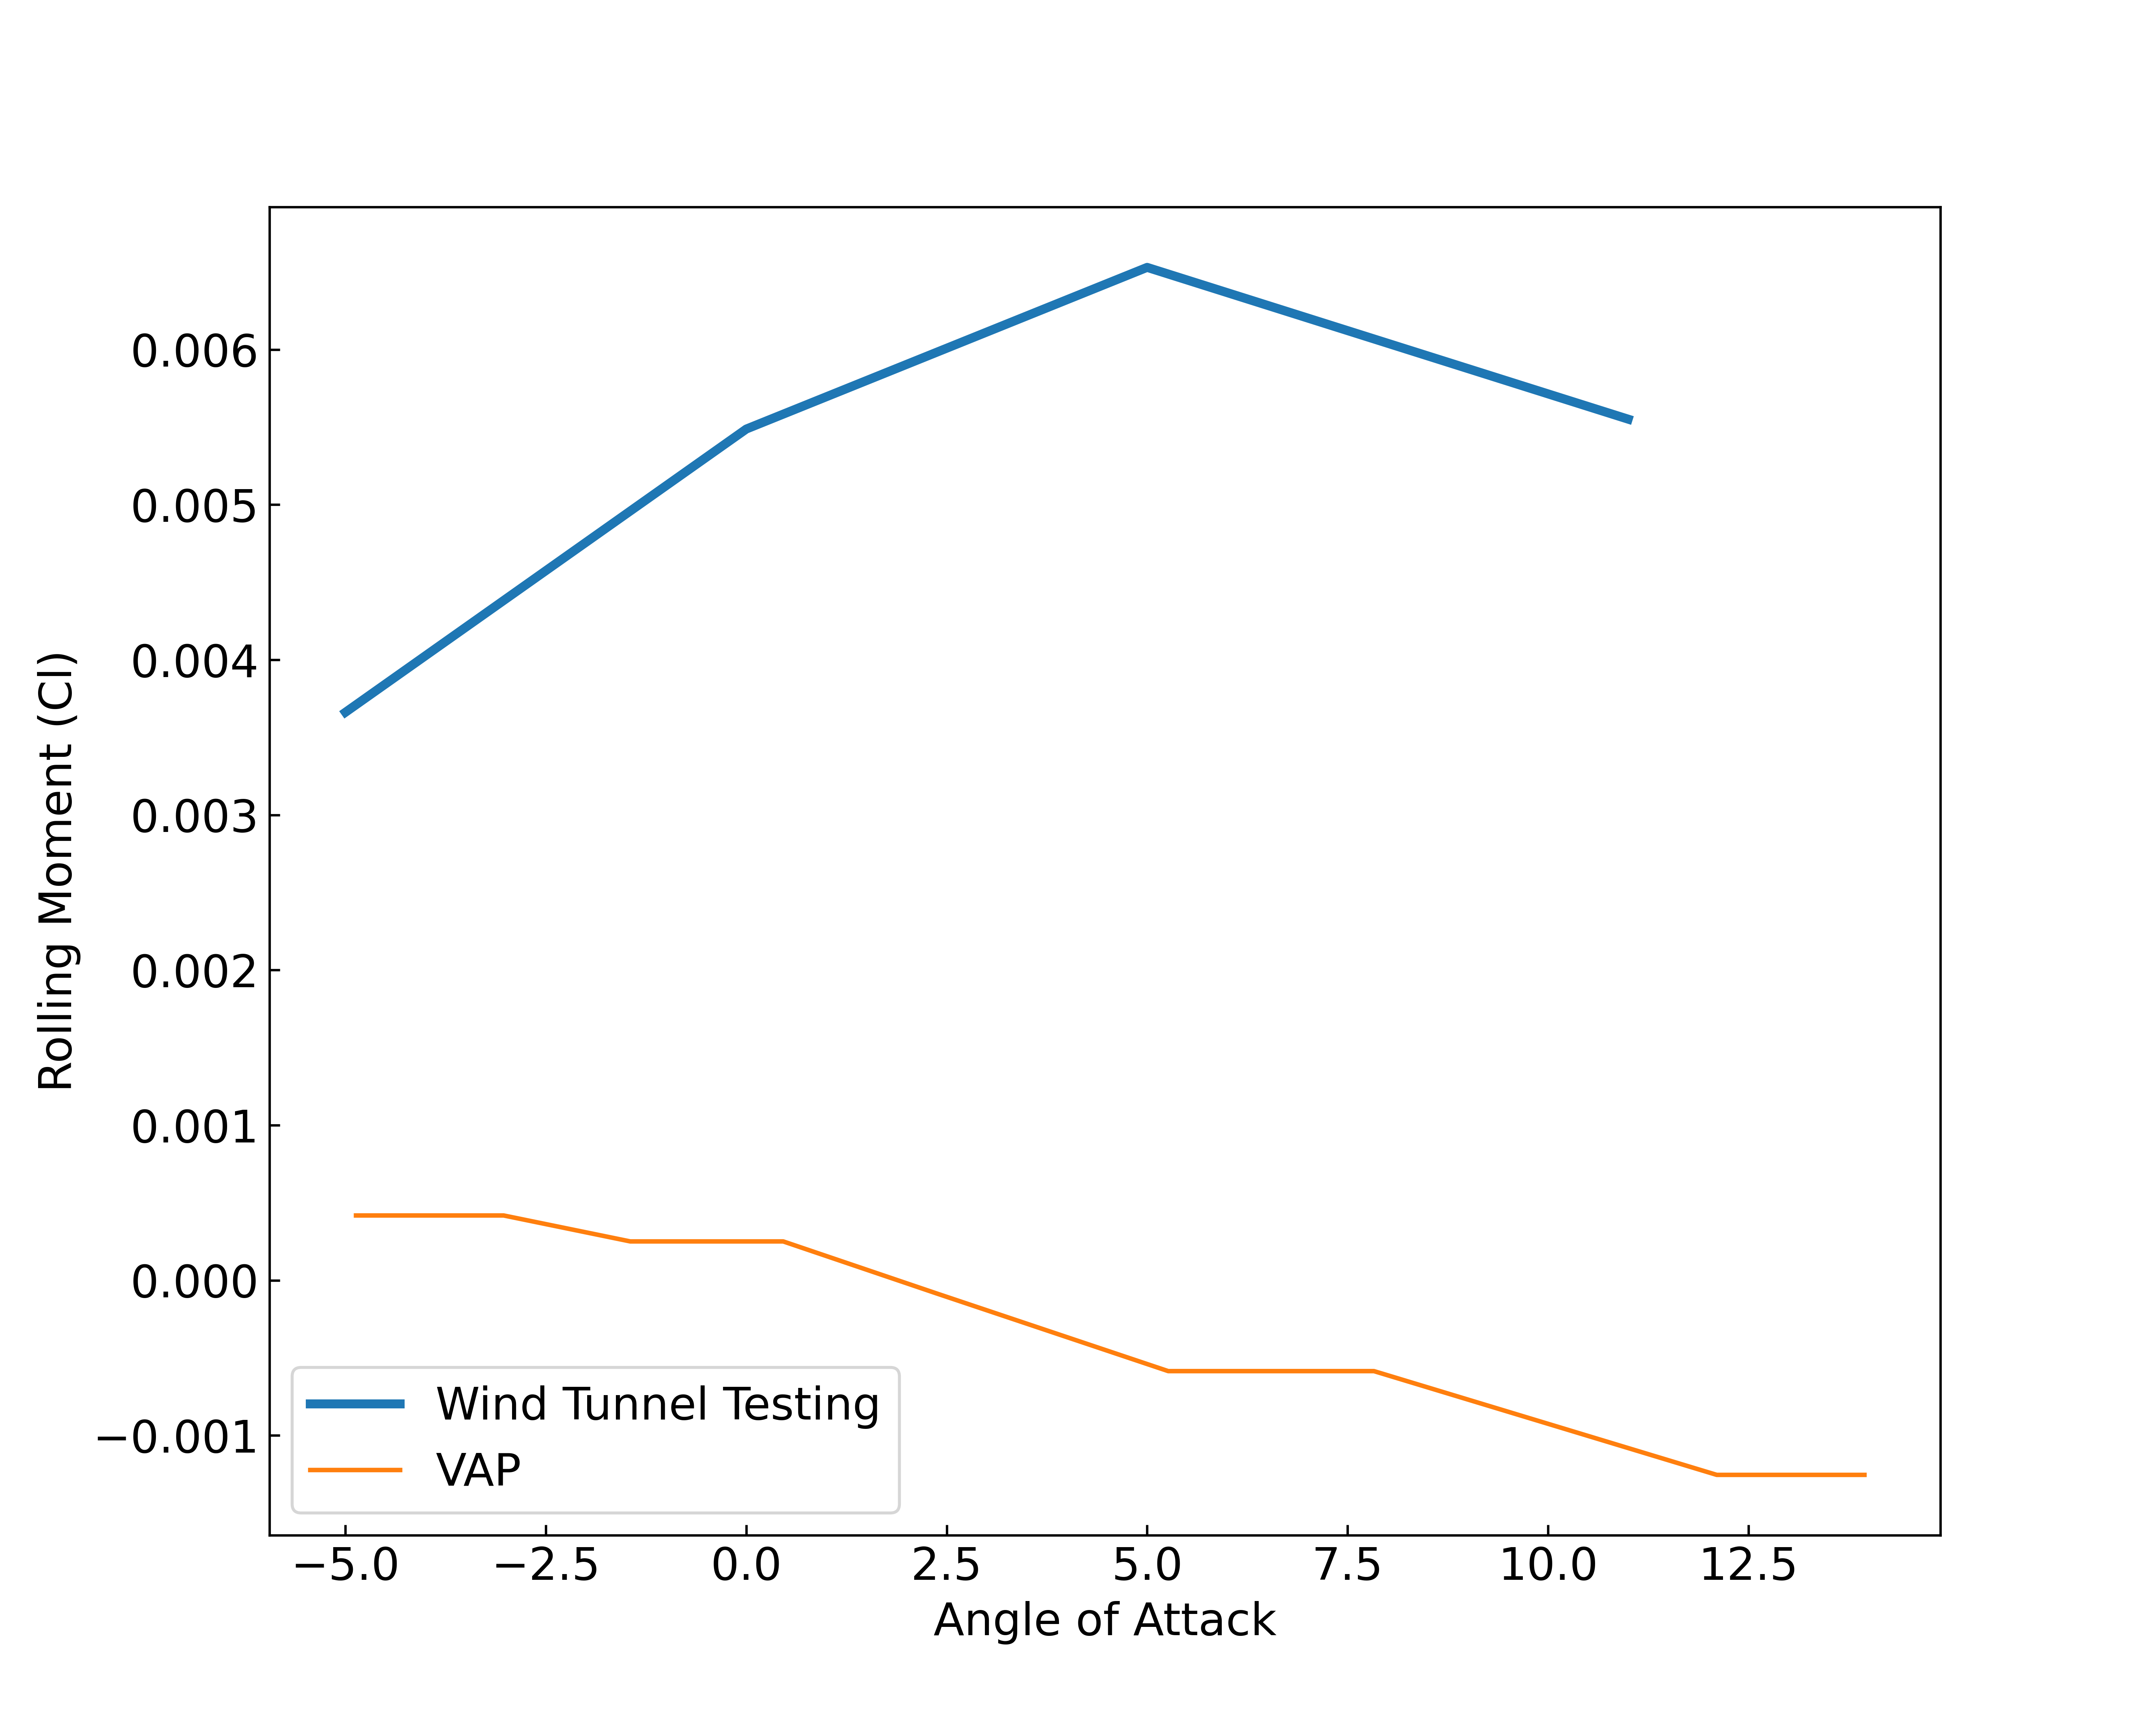
\includegraphics[width=\textwidth]{05_Results/VAP/noProp/Cl/20ms_6000RPM_Cl.png}
        \caption{Rolling Moment Coefficient at 20m/s airspeed for no propeller configuration}
        \label{fig:VAP_NoProp_Cl_20ms_6000}
    \end{subfigure}
    \begin{subfigure}[b]{0.467\textwidth}
        \centering
        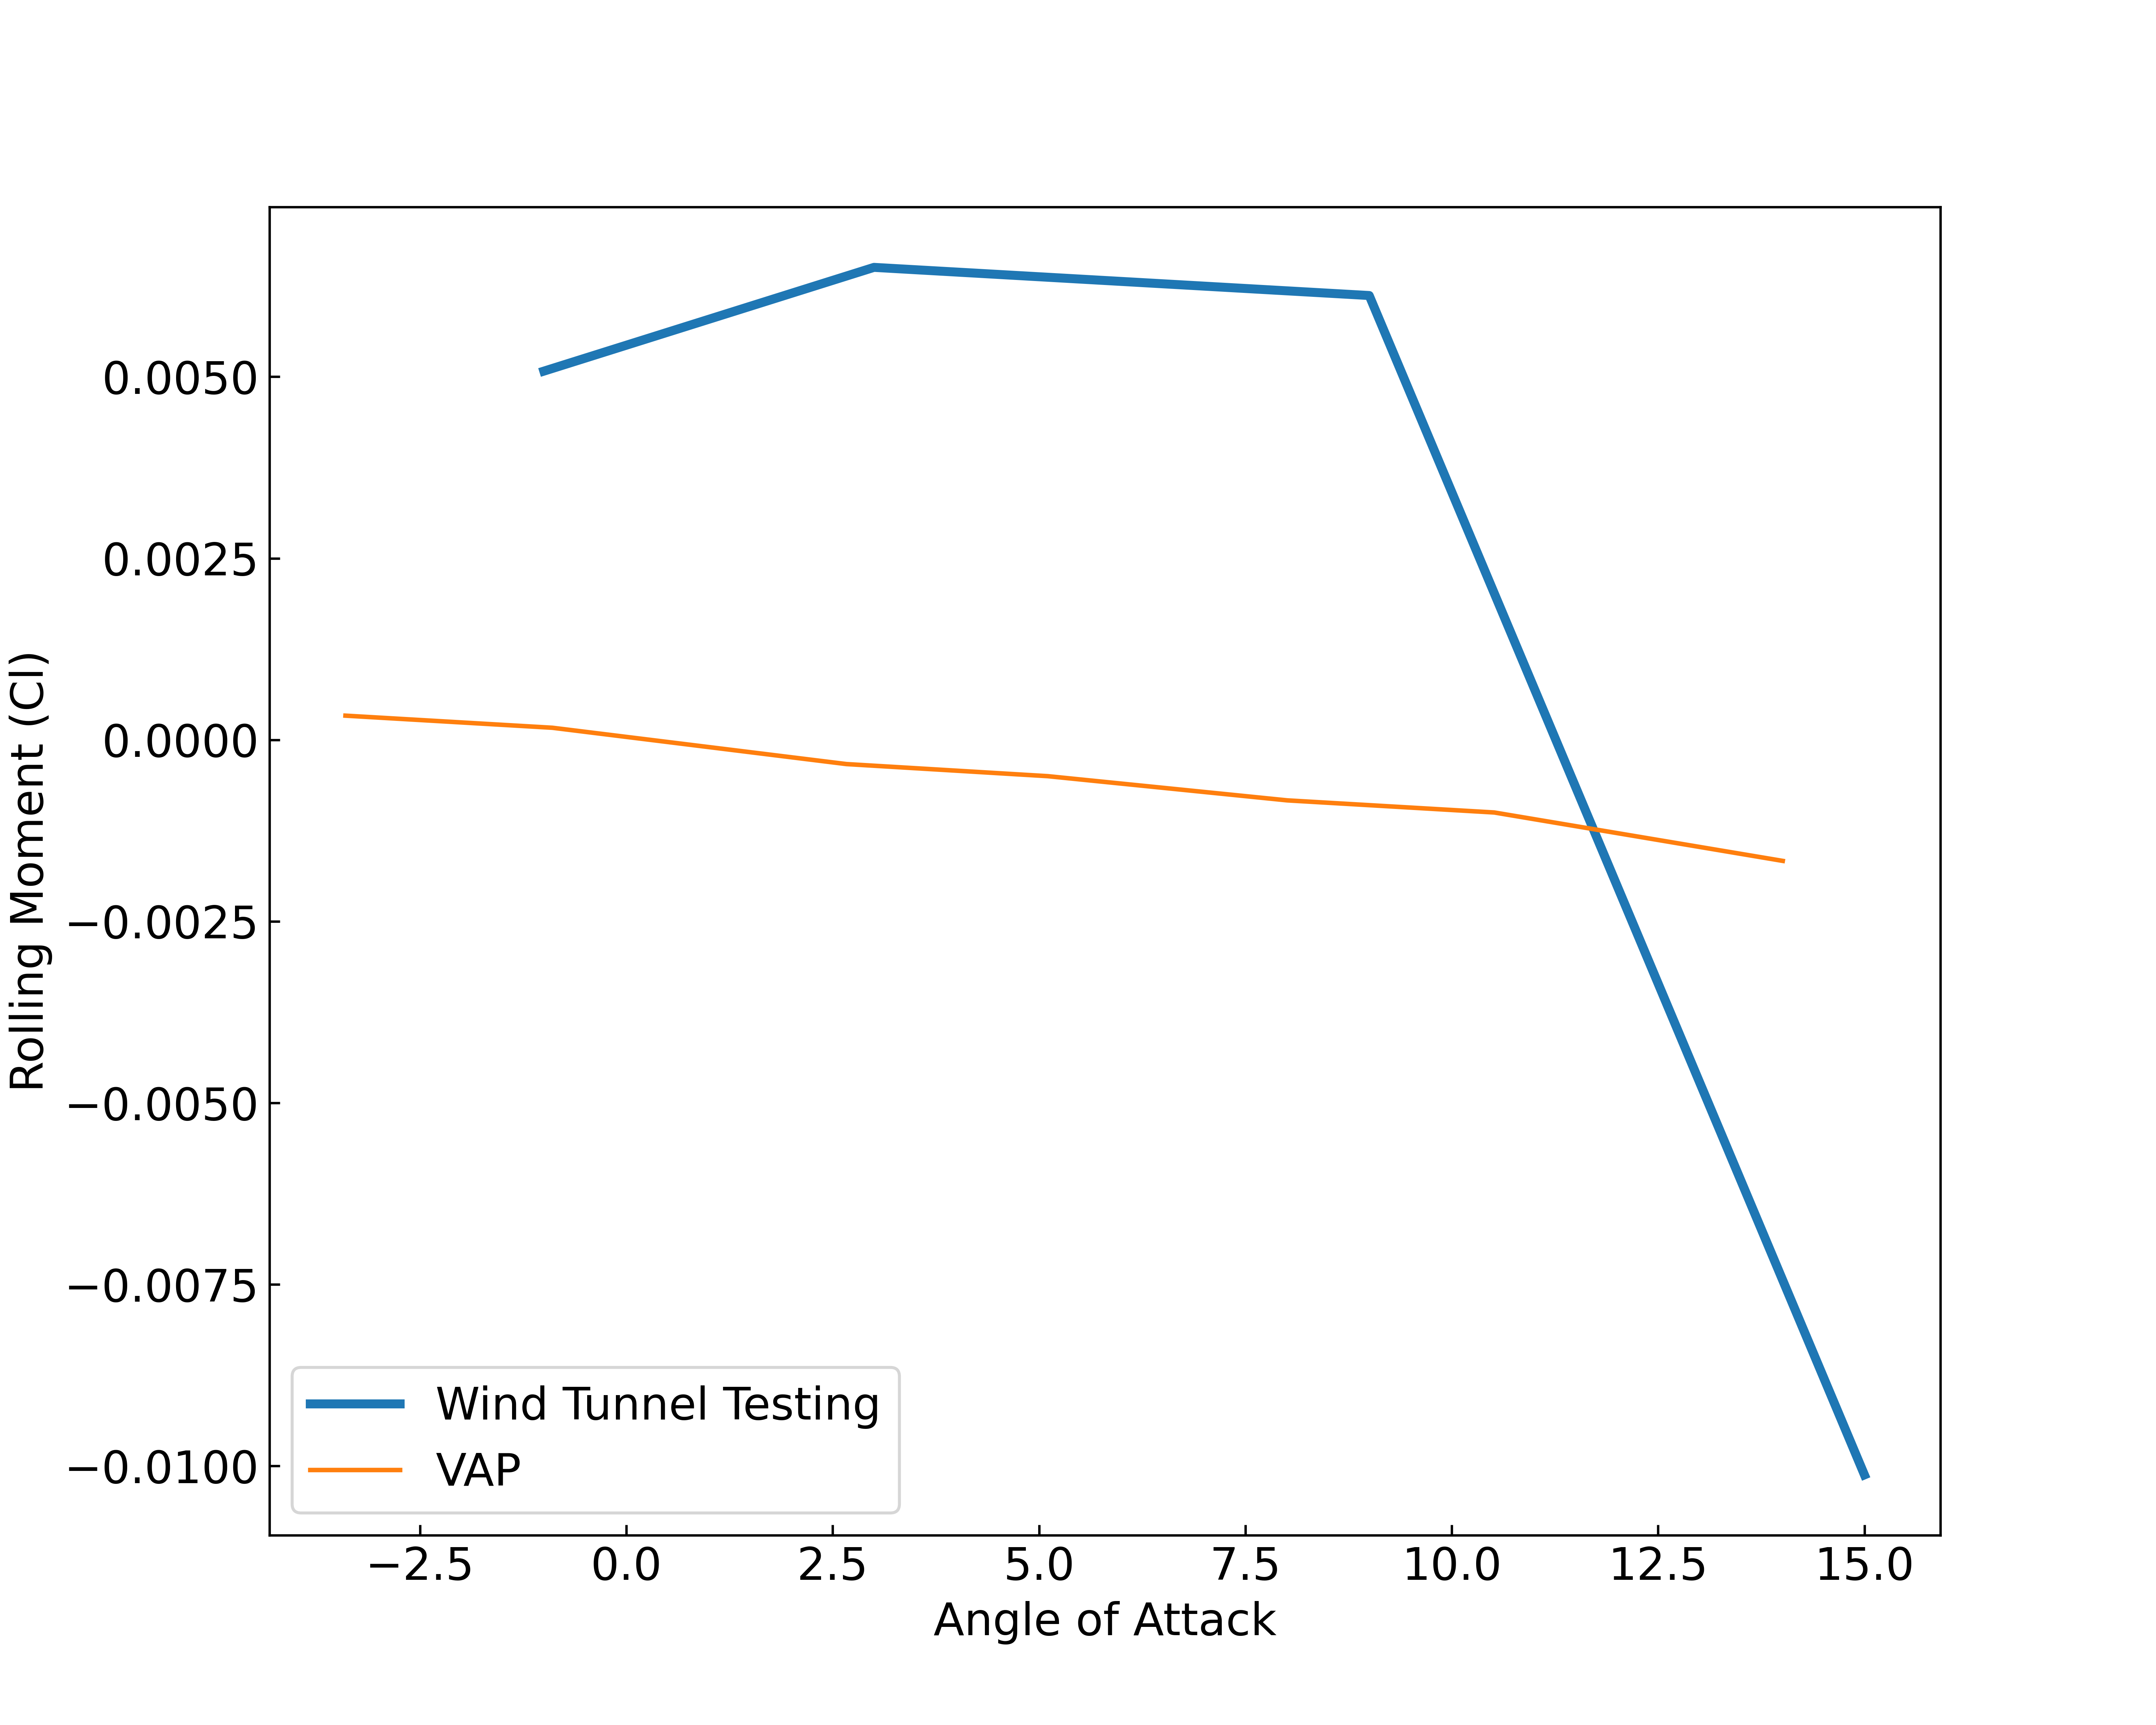
\includegraphics[width=\textwidth]{05_Results/VAP/noProp/Cl/20ms_11000RPM_Cl.png}
        \caption{Rolling Moment Coefficient at 20m/s airspeed for no propeller configuration}
        \label{fig:VAP_NoProp_Cl_20ms_11000}
    \end{subfigure}
\end{figure}


Figures \ref{fig:VAP_NoProp_Cm_10ms_6000} to \ref{fig:VAP_NoProp_Cm_20ms_11000} show that the pitching moment has similar slopes between the VAP 3.5 and wind tunnel results. This indicates a similar $C_{m_{\alpha}}$, which describes the stability of the model in terms of the pitching moment. However, the magnitude of the pitching moment force is incorrectly calculated by the VAP 3.5 software. VAP 3.5 does not predict the forces at \acrshort{AoA}s lower than 0$^\circ$ well. Hence these discrepancies are expected. Results indicate that further development is needed, and refinement of the geometry's detail could account for the offset seen in the pitching moment. 


\begin{figure}[H]
    \centering
    \begin{subfigure}[b]{0.467\textwidth}
        \centering
        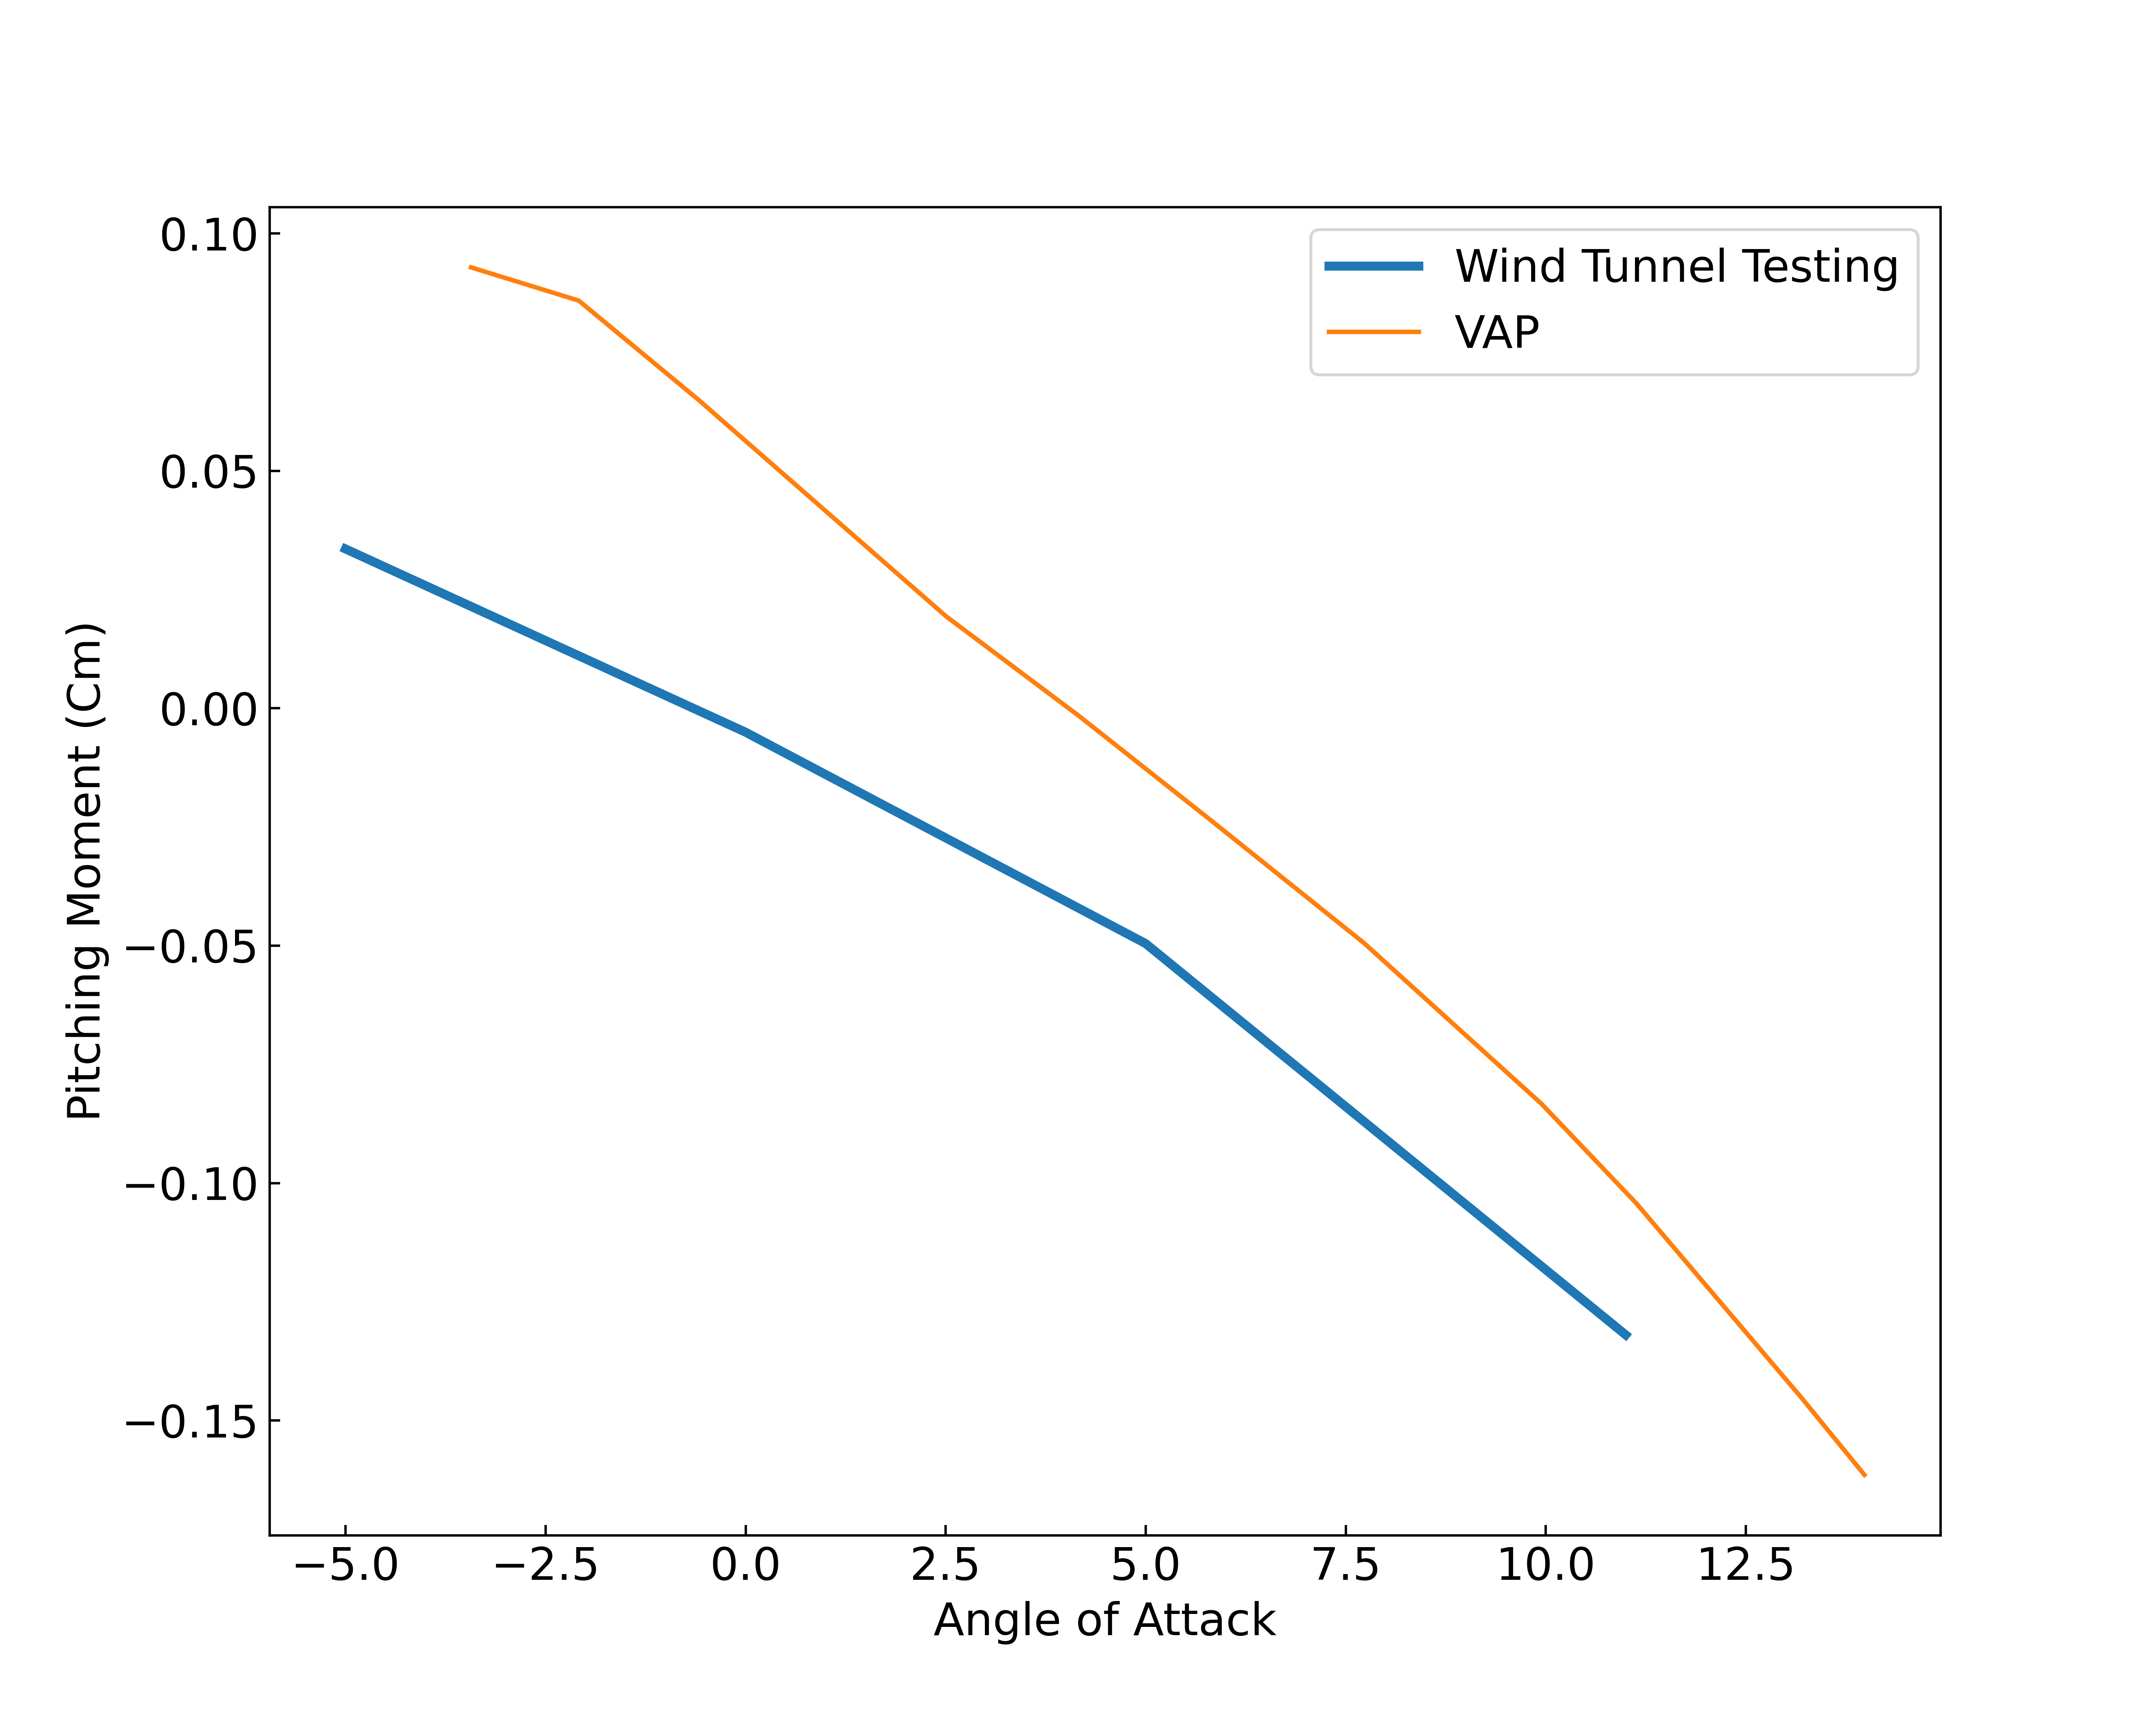
\includegraphics[width=\textwidth]{05_Results/VAP/noProp/Cm/10ms_6000RPM_Cm.png}
        \caption{Pitching Moment Coefficient at 10m/s airspeed for no propeller configuration}
        \label{fig:VAP_NoProp_Cm_10ms_6000}
    \end{subfigure}
    \begin{subfigure}[b]{0.467\textwidth}
        \centering
        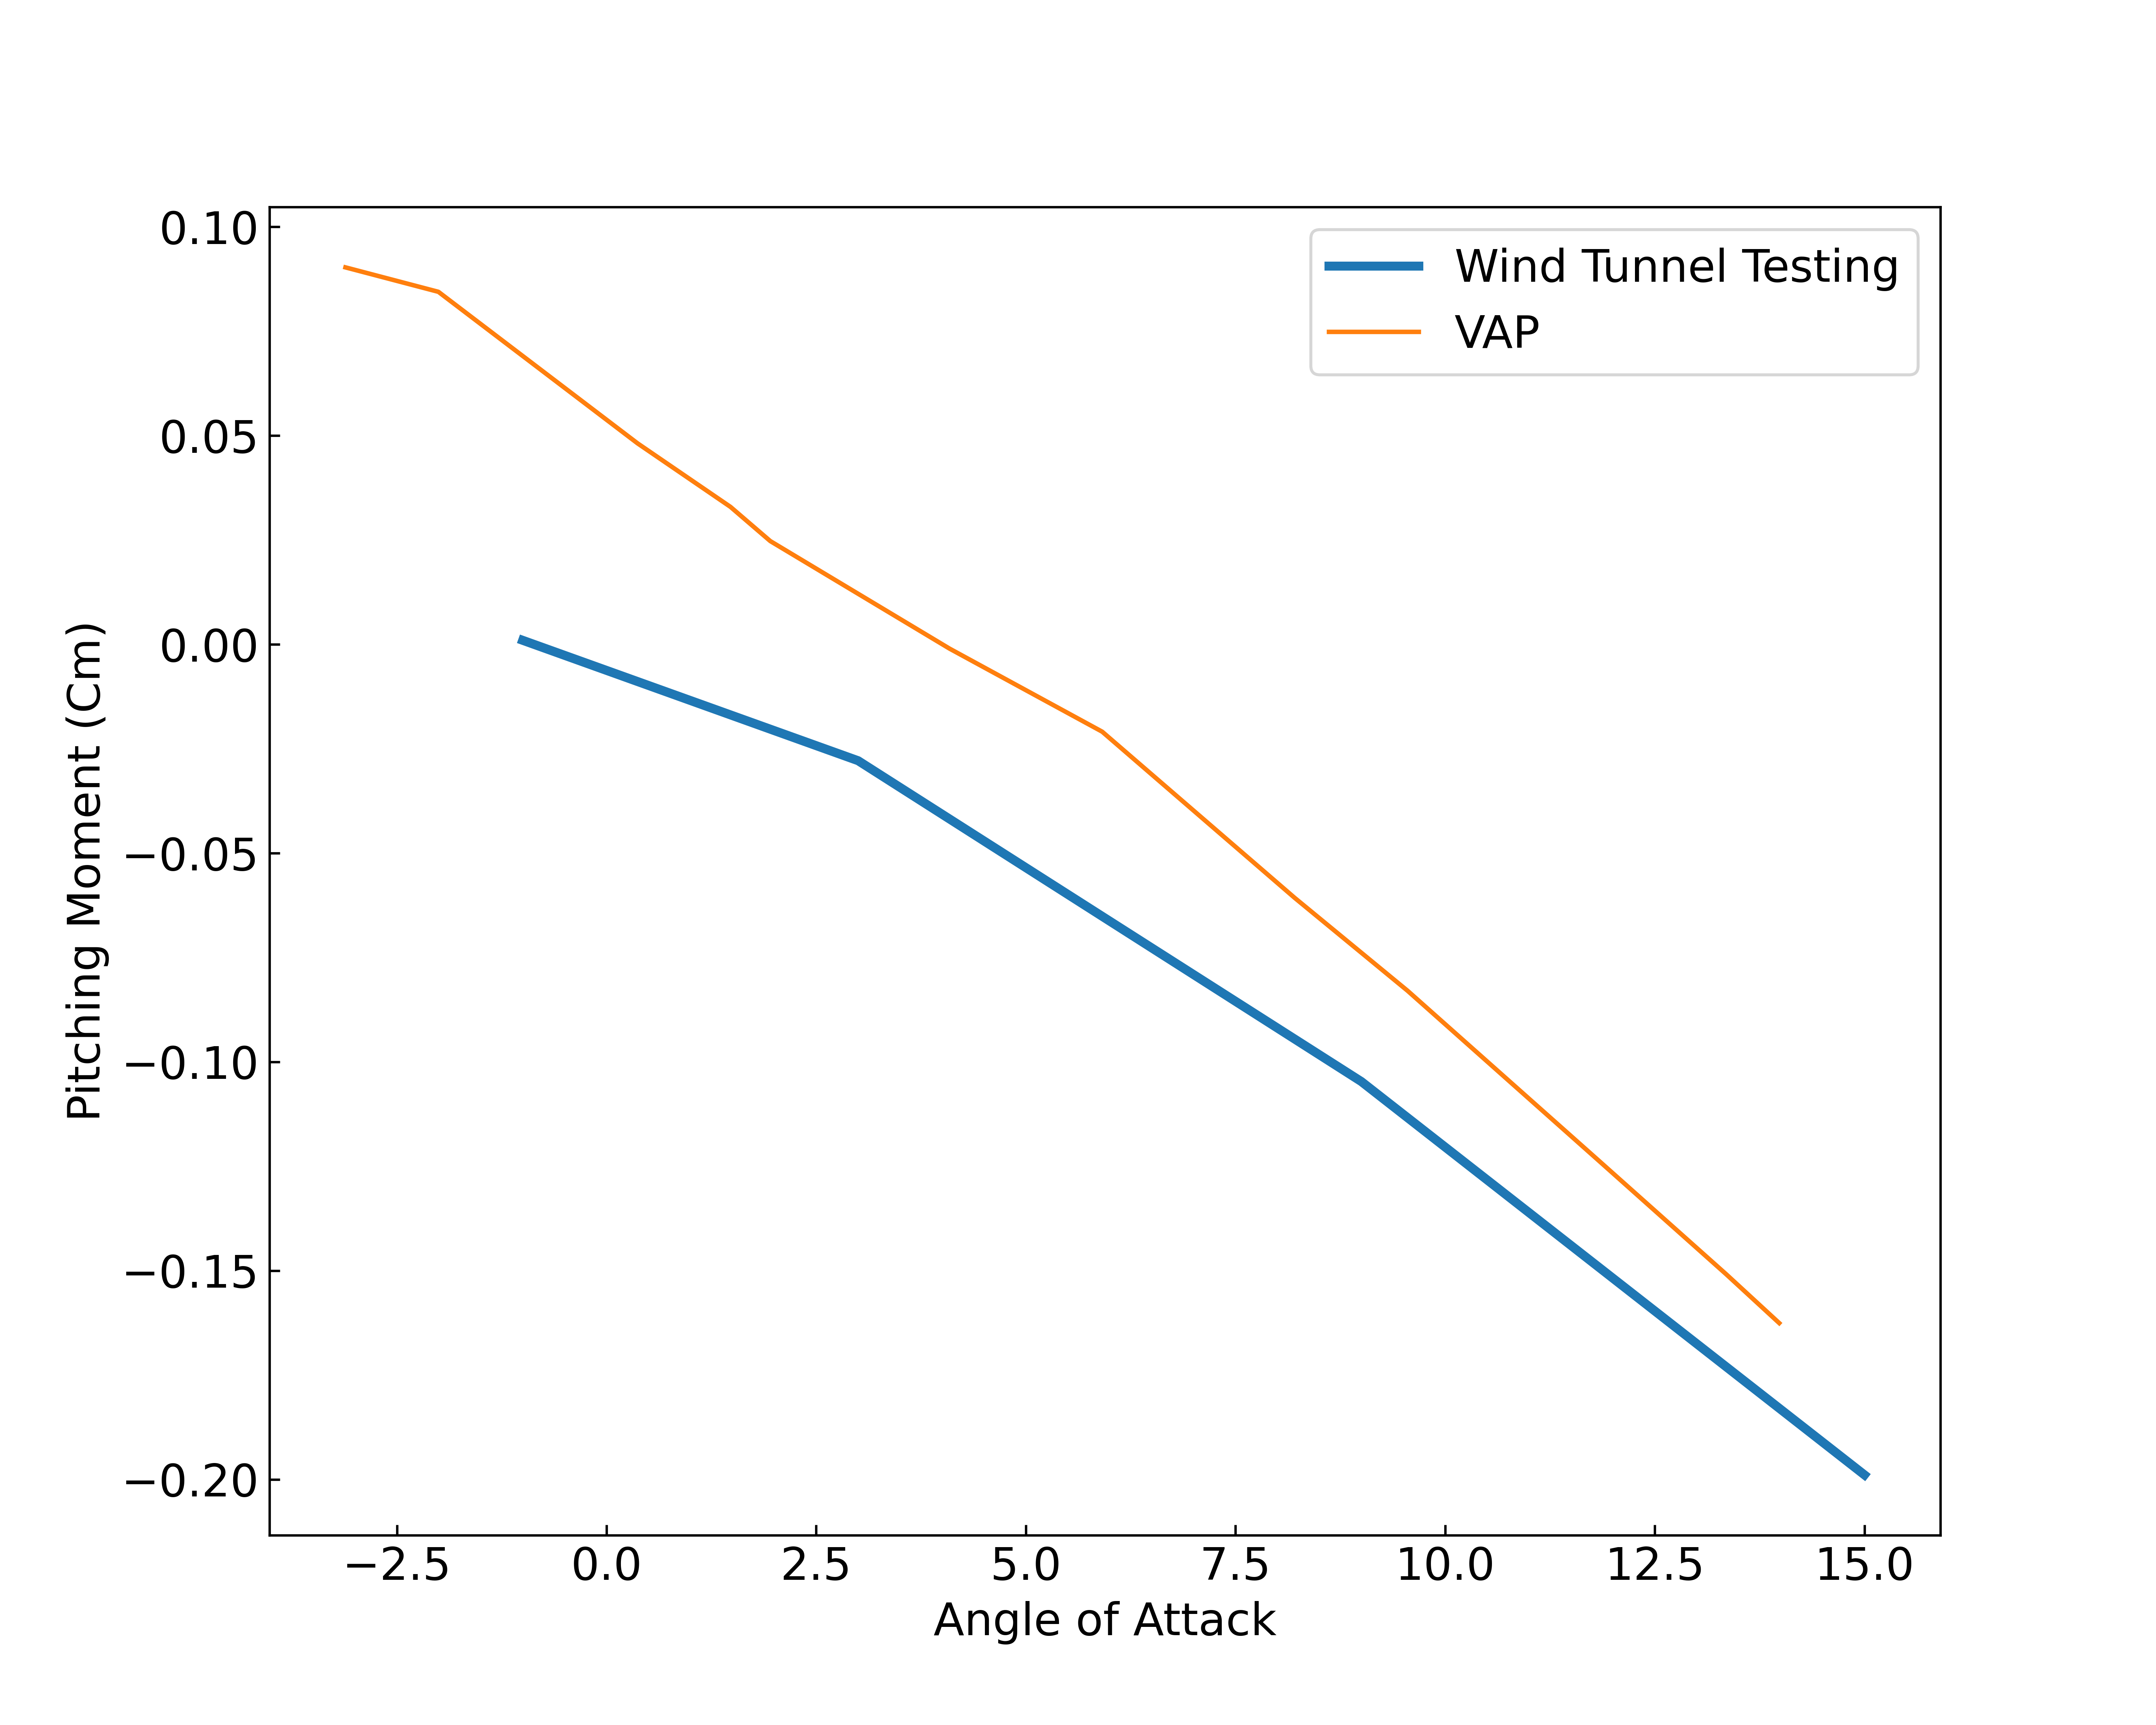
\includegraphics[width=\textwidth]{05_Results/VAP/noProp/Cm/10ms_11000RPM_Cm.png}
        \caption{Pitching Moment Coefficient at 10m/s airspeed for no propeller configuration}
        \label{fig:VAP_NoProp_Cm_10ms_11000}
    \end{subfigure}
    \begin{subfigure}[b]{0.467\textwidth}
        \centering
        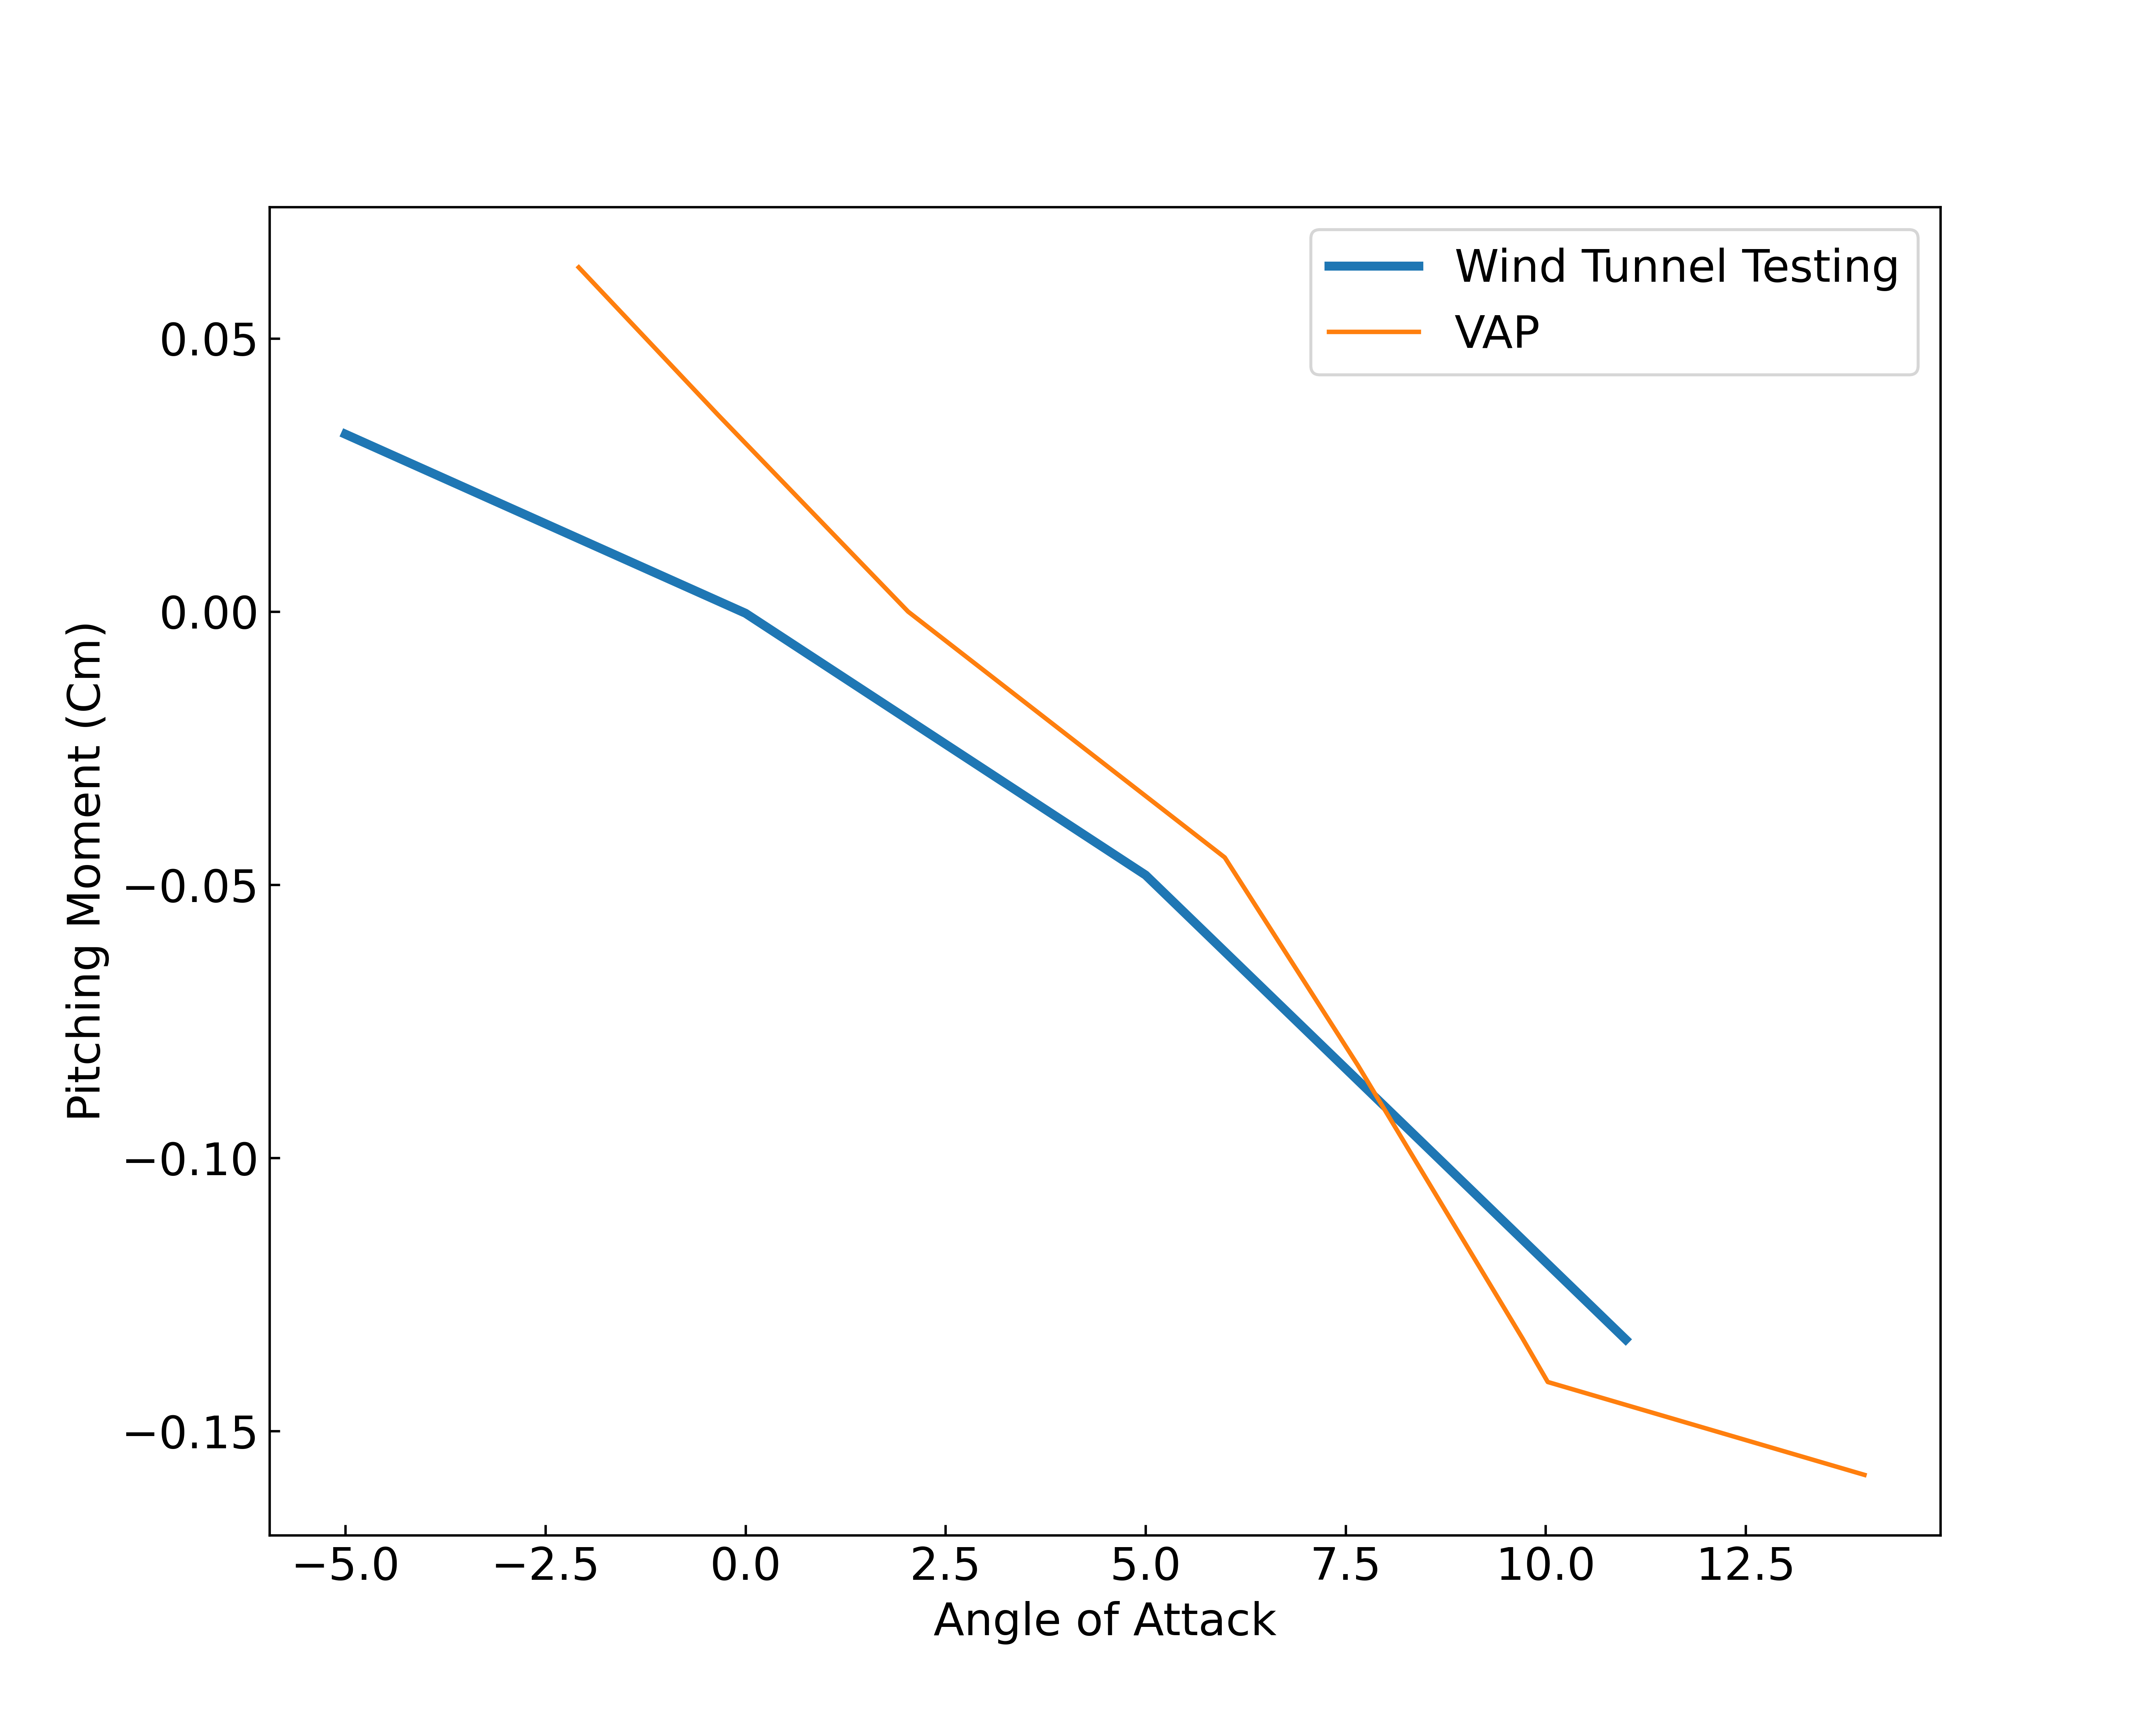
\includegraphics[width=\textwidth]{05_Results/VAP/noProp/Cm/20ms_6000RPM_Cm.png}
        \caption{Pitching Moment Coefficient at 20m/s airspeed for no propeller configuration}
        \label{fig:VAP_NoProp_Cm_20ms_6000}
    \end{subfigure}
    \begin{subfigure}[b]{0.467\textwidth}
        \centering
        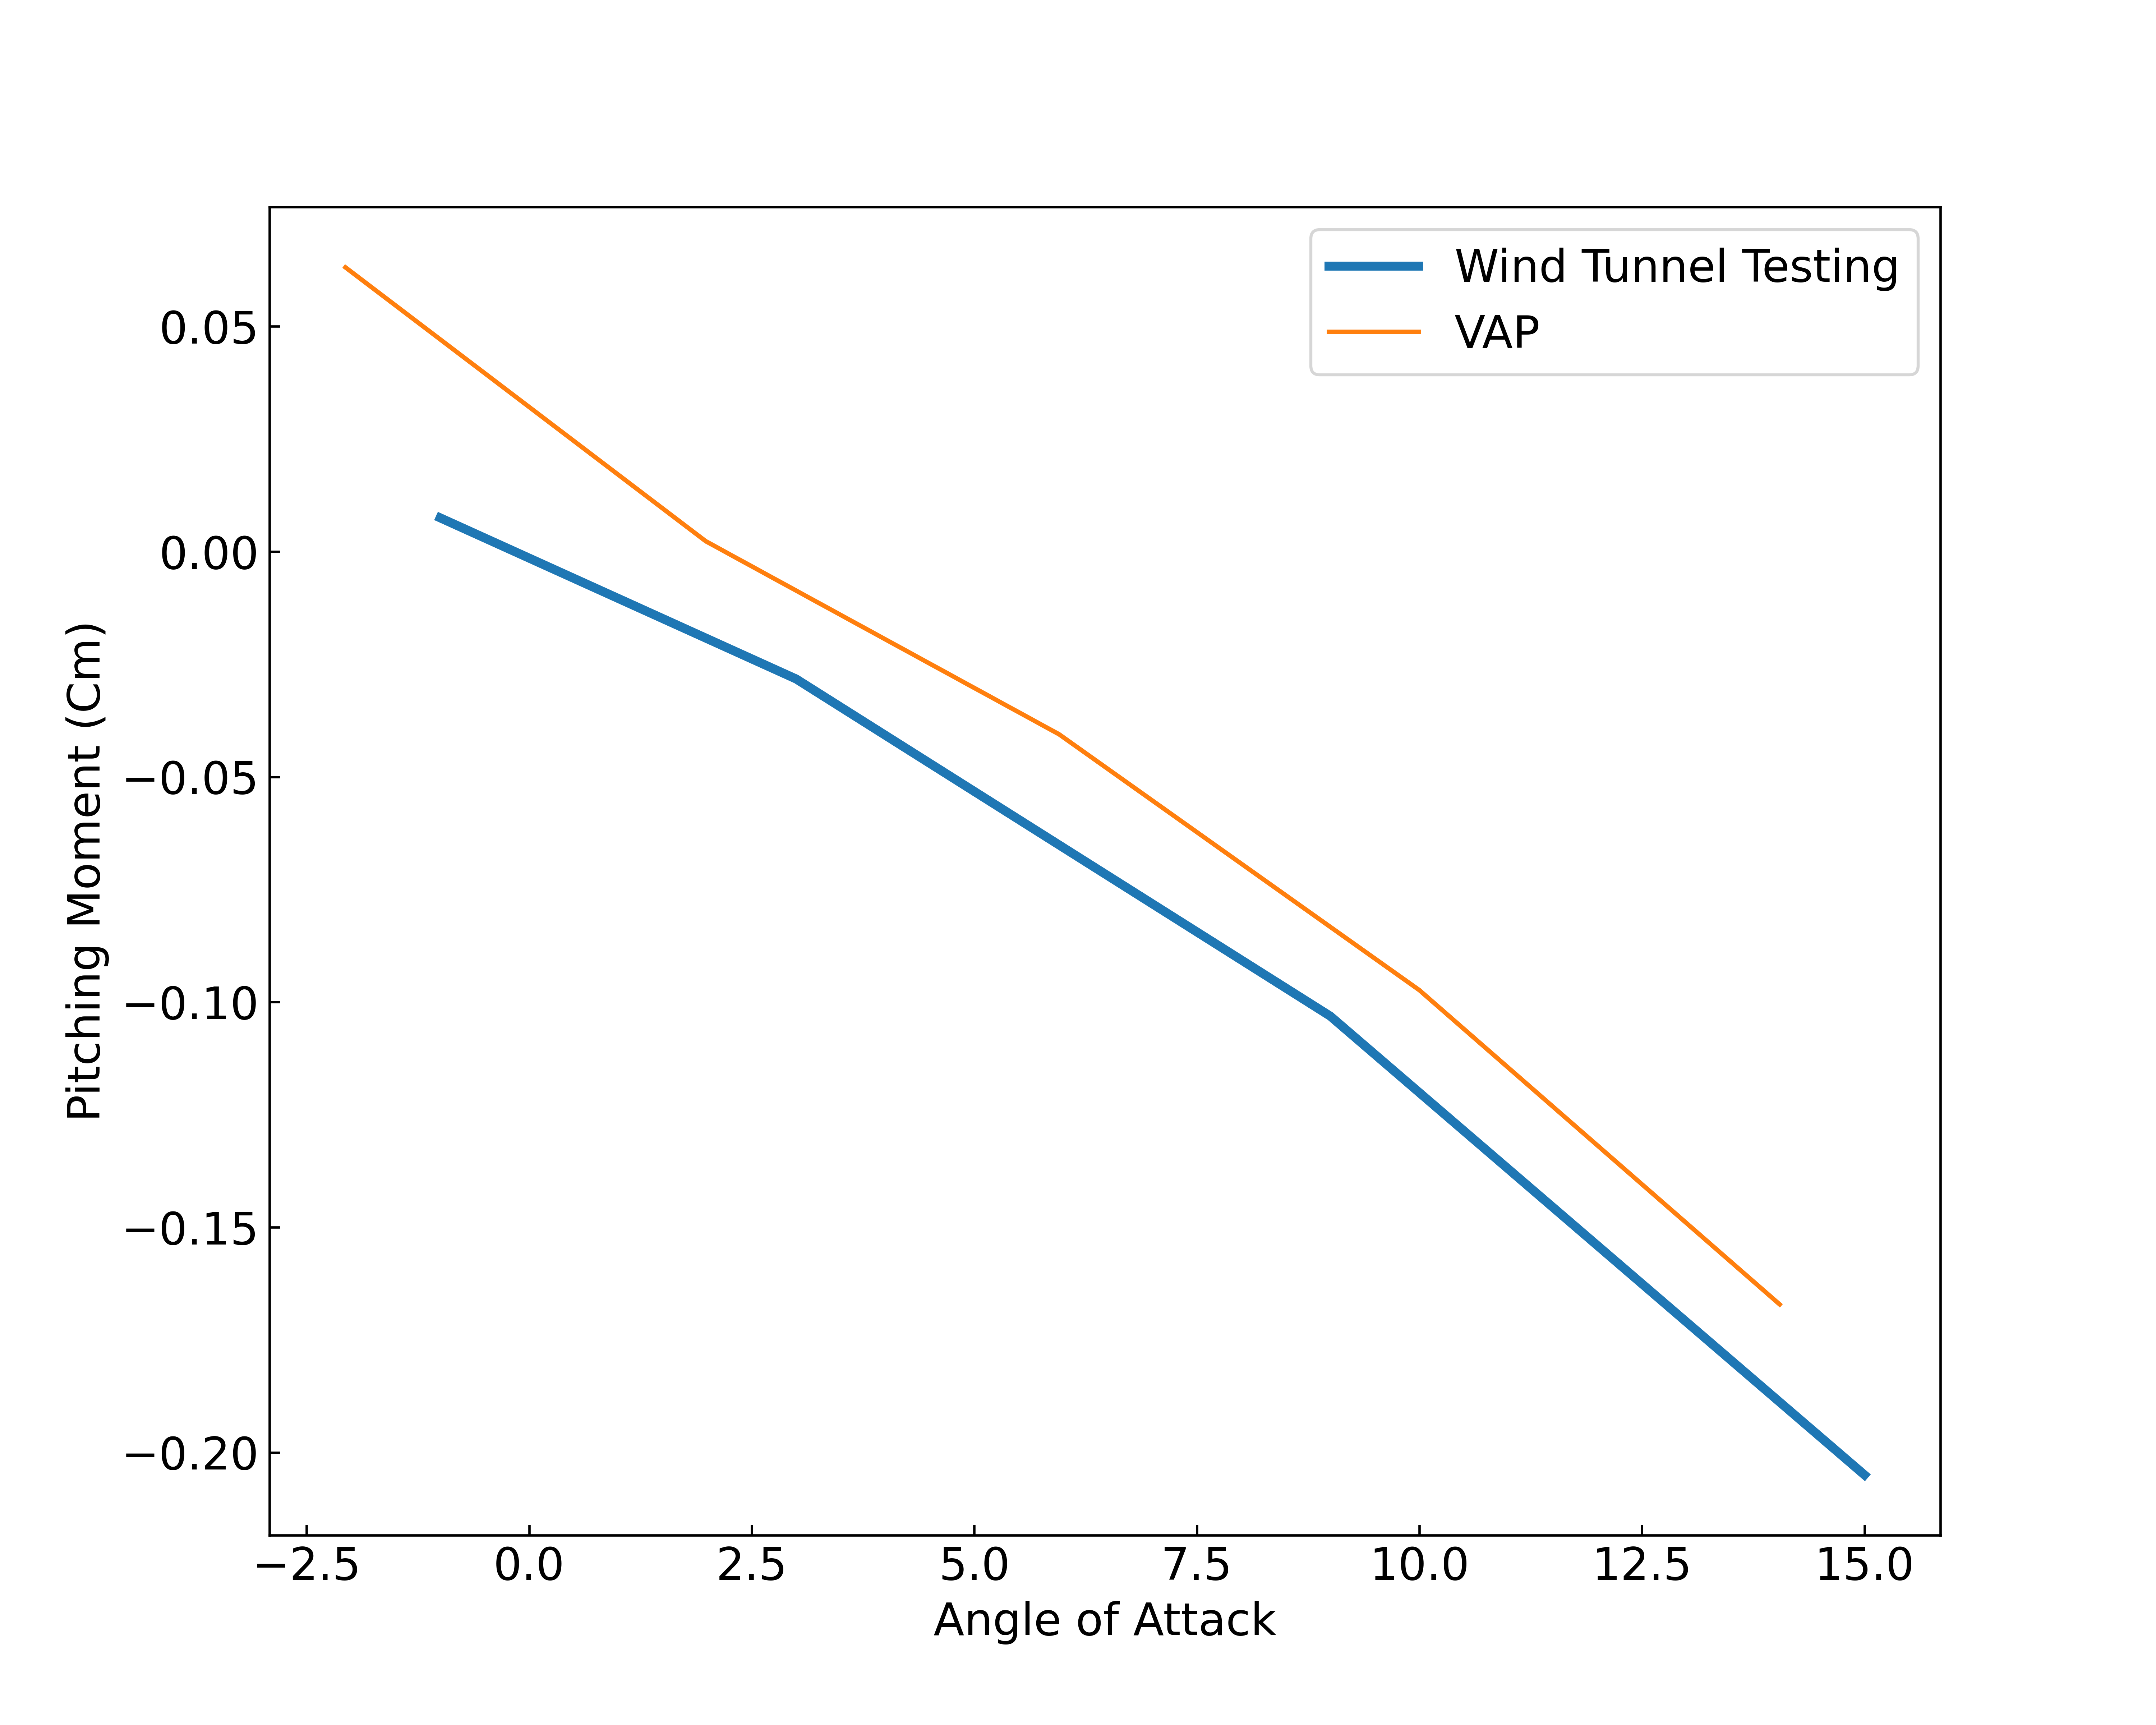
\includegraphics[width=\textwidth]{05_Results/VAP/noProp/Cm/20ms_11000RPM_Cm.png}
        \caption{Pitching Moment Coefficient at 20m/s airspeed for no propeller configuration}
        \label{fig:VAP_NoProp_Cm_20ms_11000}
    \end{subfigure}
\end{figure}

Figures \ref{fig:VAP_noProp_Cn_10ms_6000} to \ref{fig:VAP_noProp_Cn_20ms_11000} show the yawing moment coefficient for the no propeller configuration.

%\todo{HELP}

\begin{figure}[H]
    \centering
    \begin{subfigure}[b]{0.467\textwidth}
        \centering
        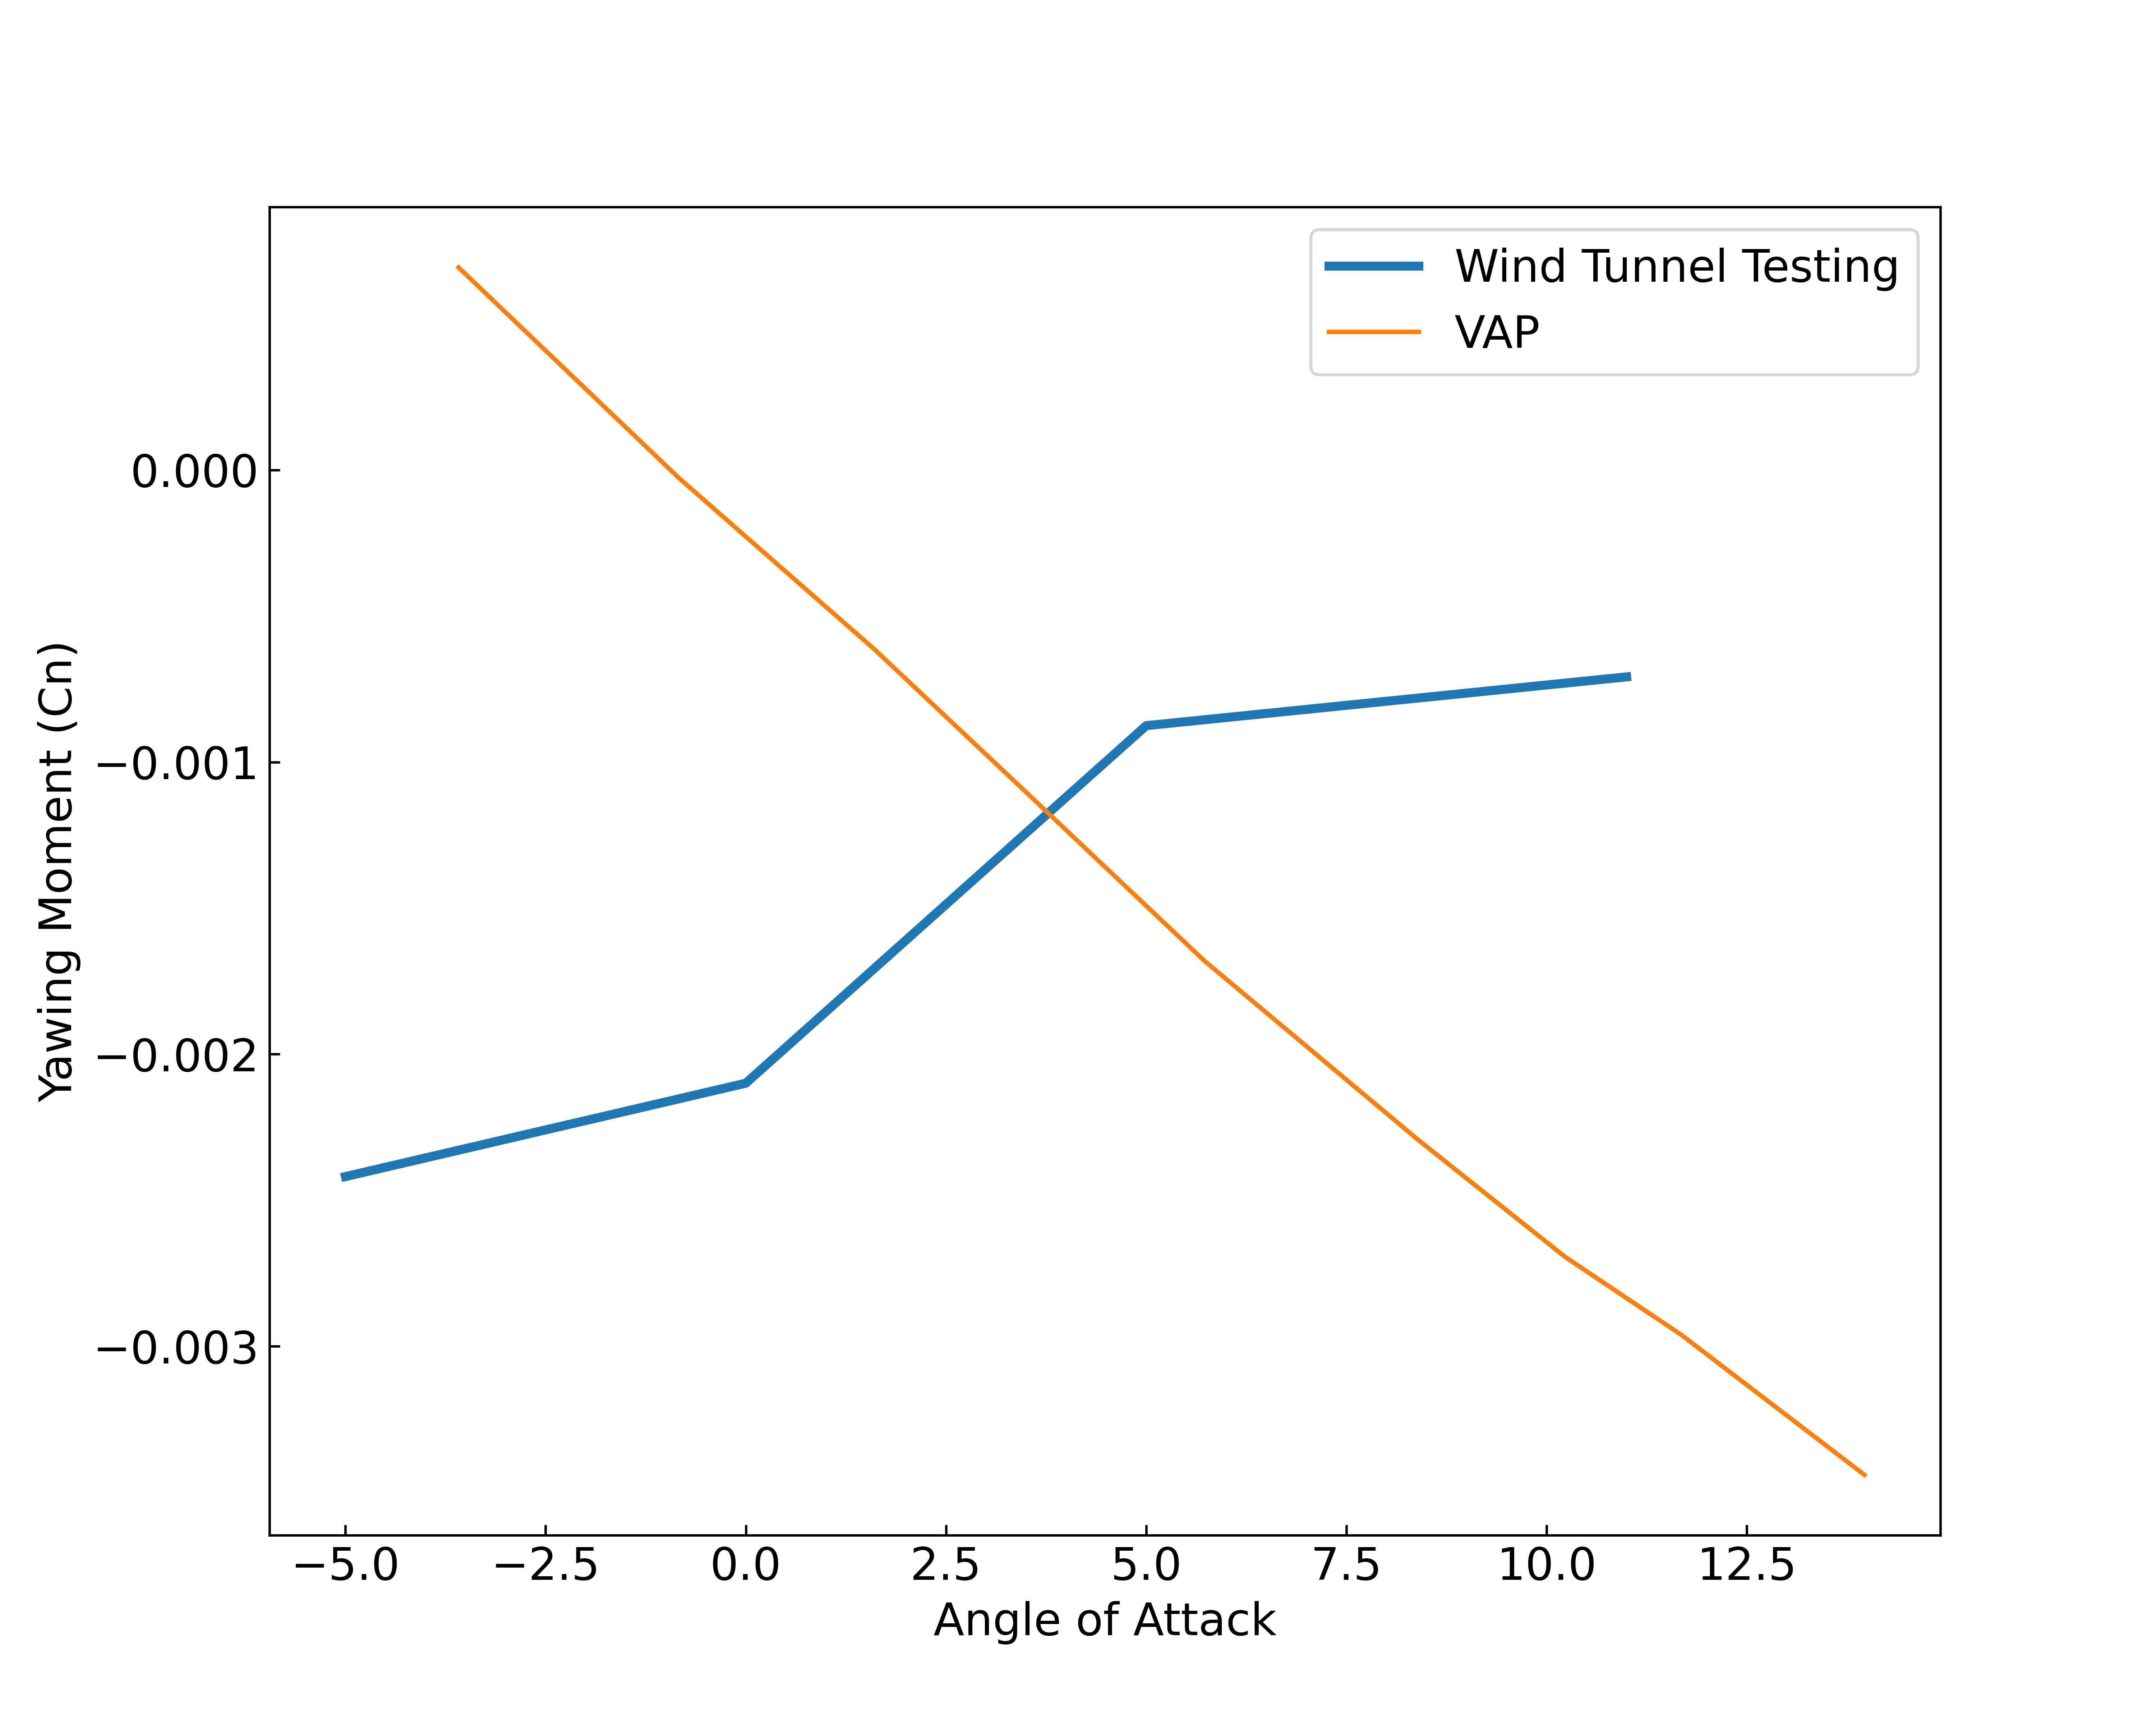
\includegraphics[width=\textwidth]{05_Results/VAP/noProp/Cn/10ms_6000RPM_Cn.png}
        \caption{Yawing Moment Coefficient at 10m/s airspeed for no propeller configuration}
        \label{fig:VAP_noProp_Cn_10ms_6000}
    \end{subfigure}
    \begin{subfigure}[b]{0.467\textwidth}
        \centering
        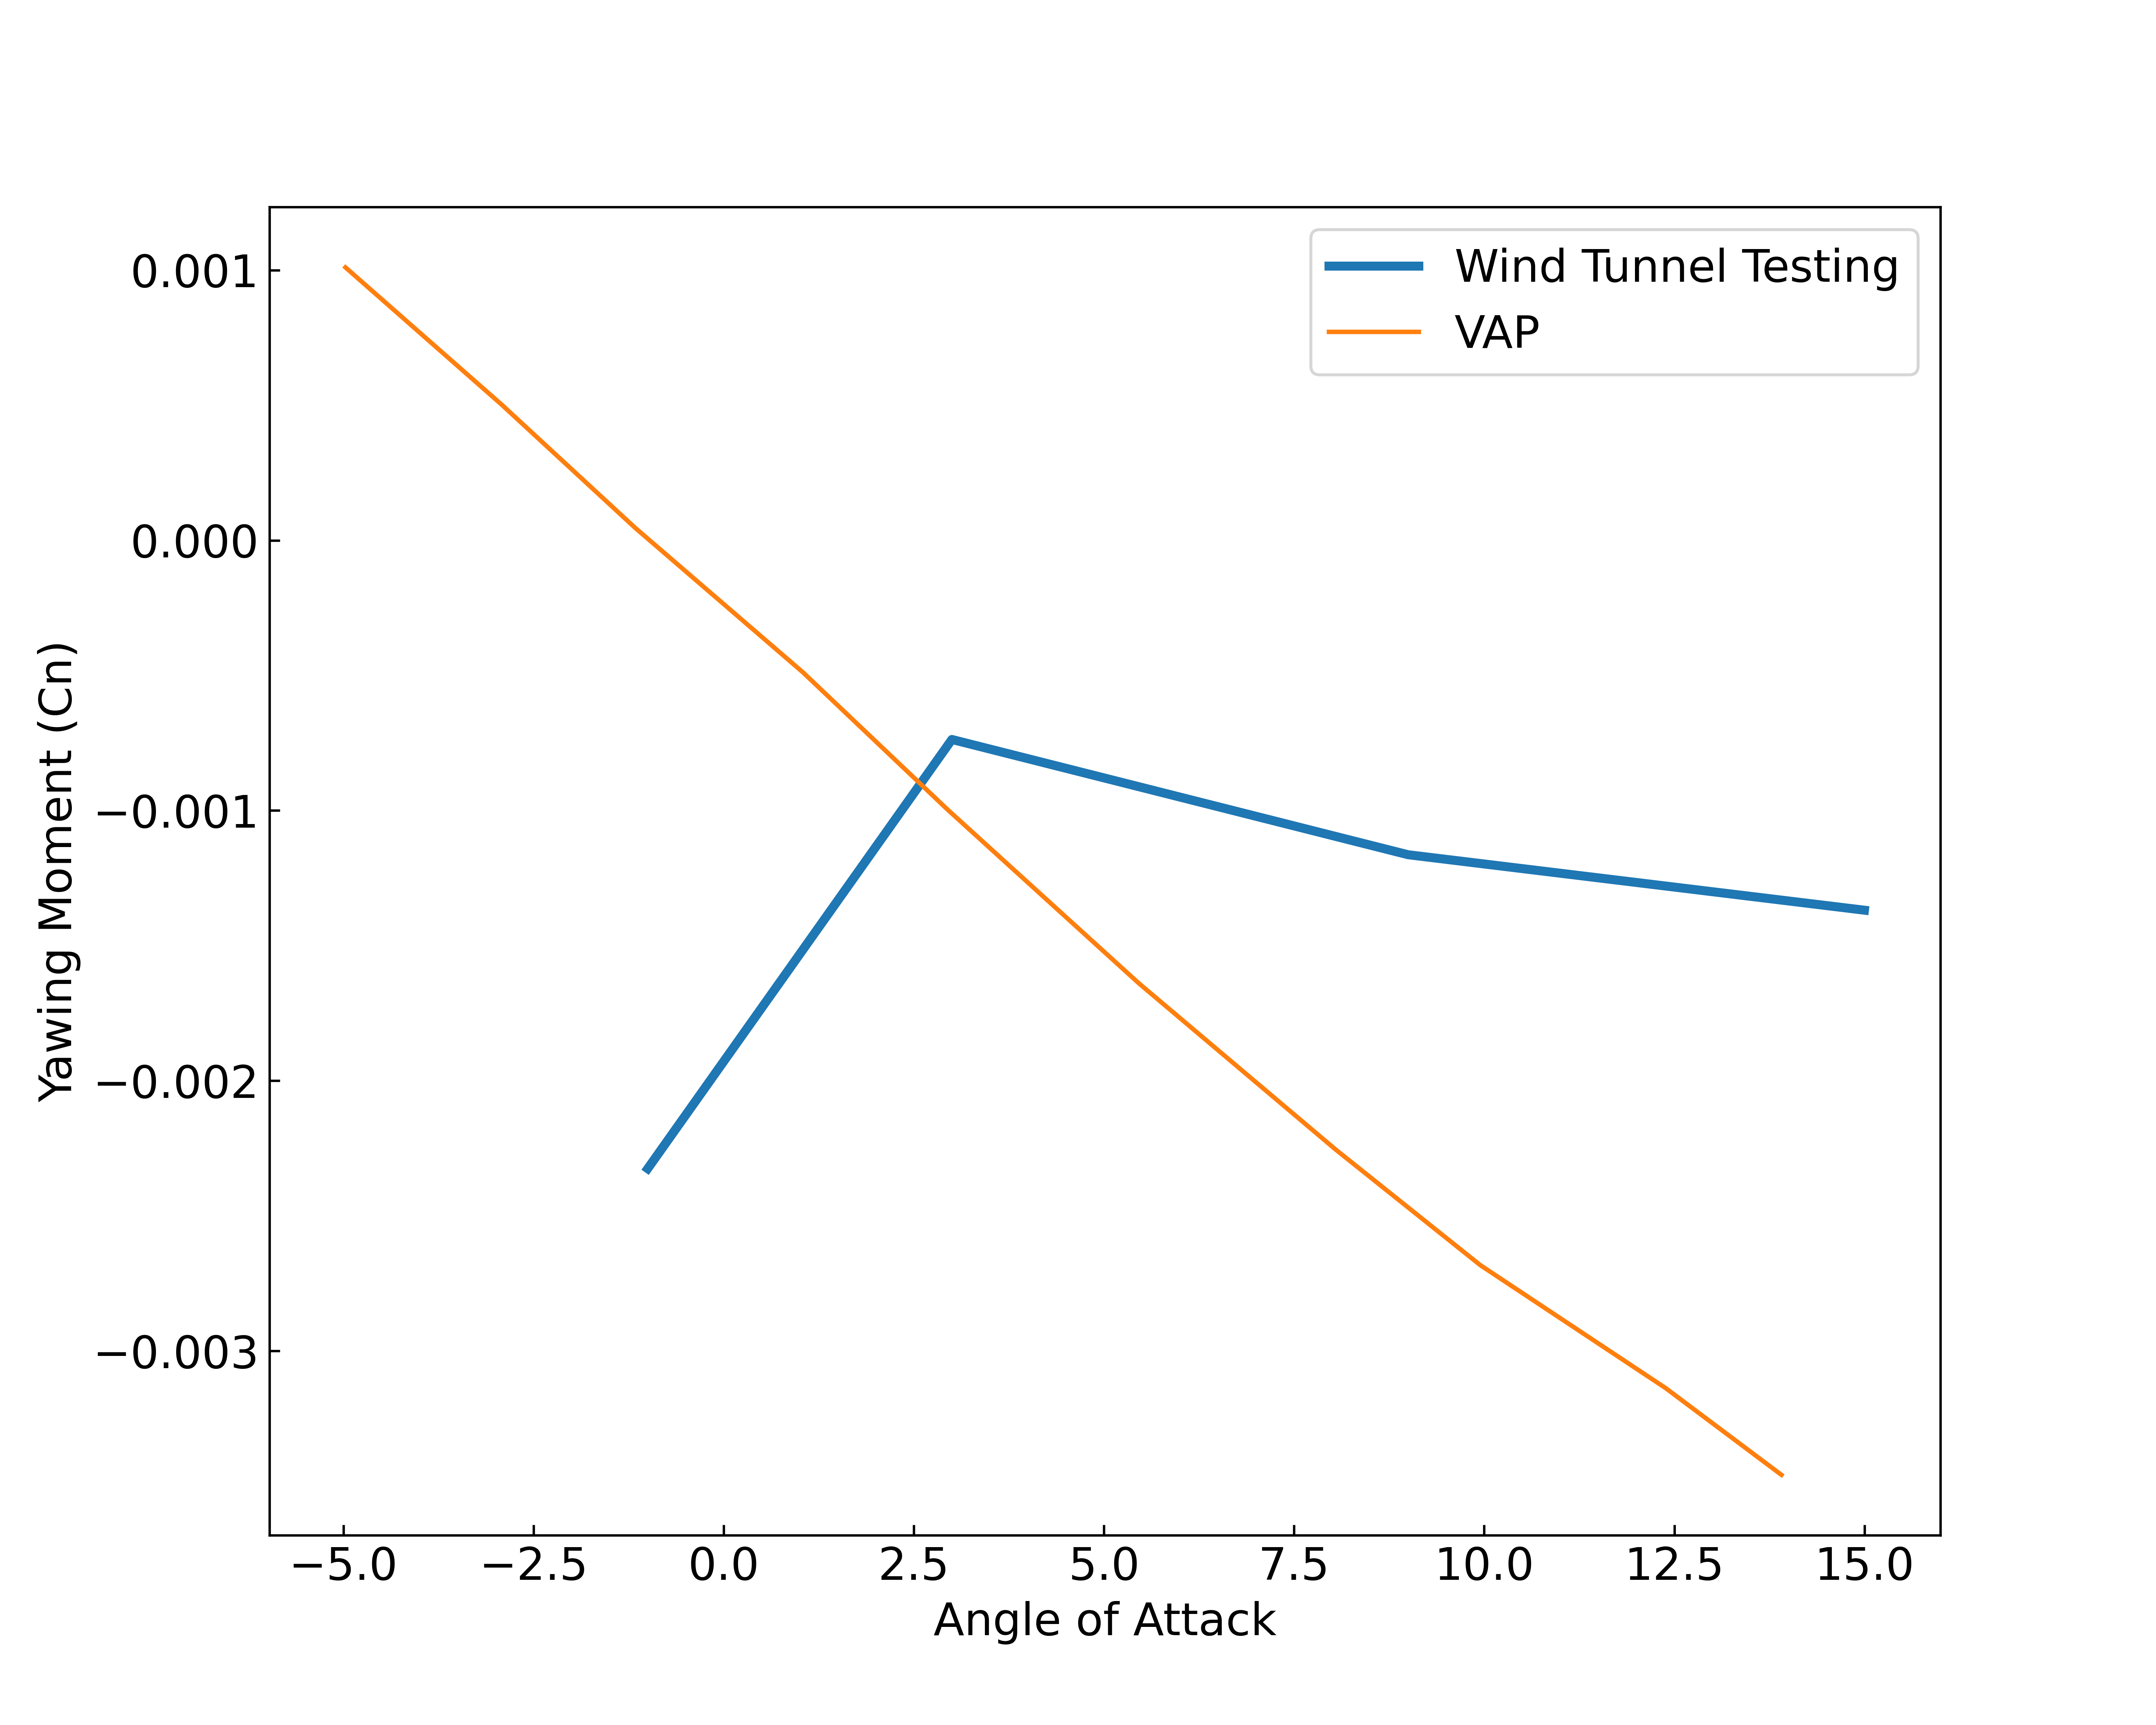
\includegraphics[width=\textwidth]{05_Results/VAP/noProp/Cn/10ms_11000RPM_Cn.png}
        \caption{Yawing Moment Coefficient at 10m/s airspeed for no propeller configuration}
        \label{fig:VAP_noProp_Cn_10ms_11000}
    \end{subfigure}
    \begin{subfigure}[b]{0.467\textwidth}
        \centering
        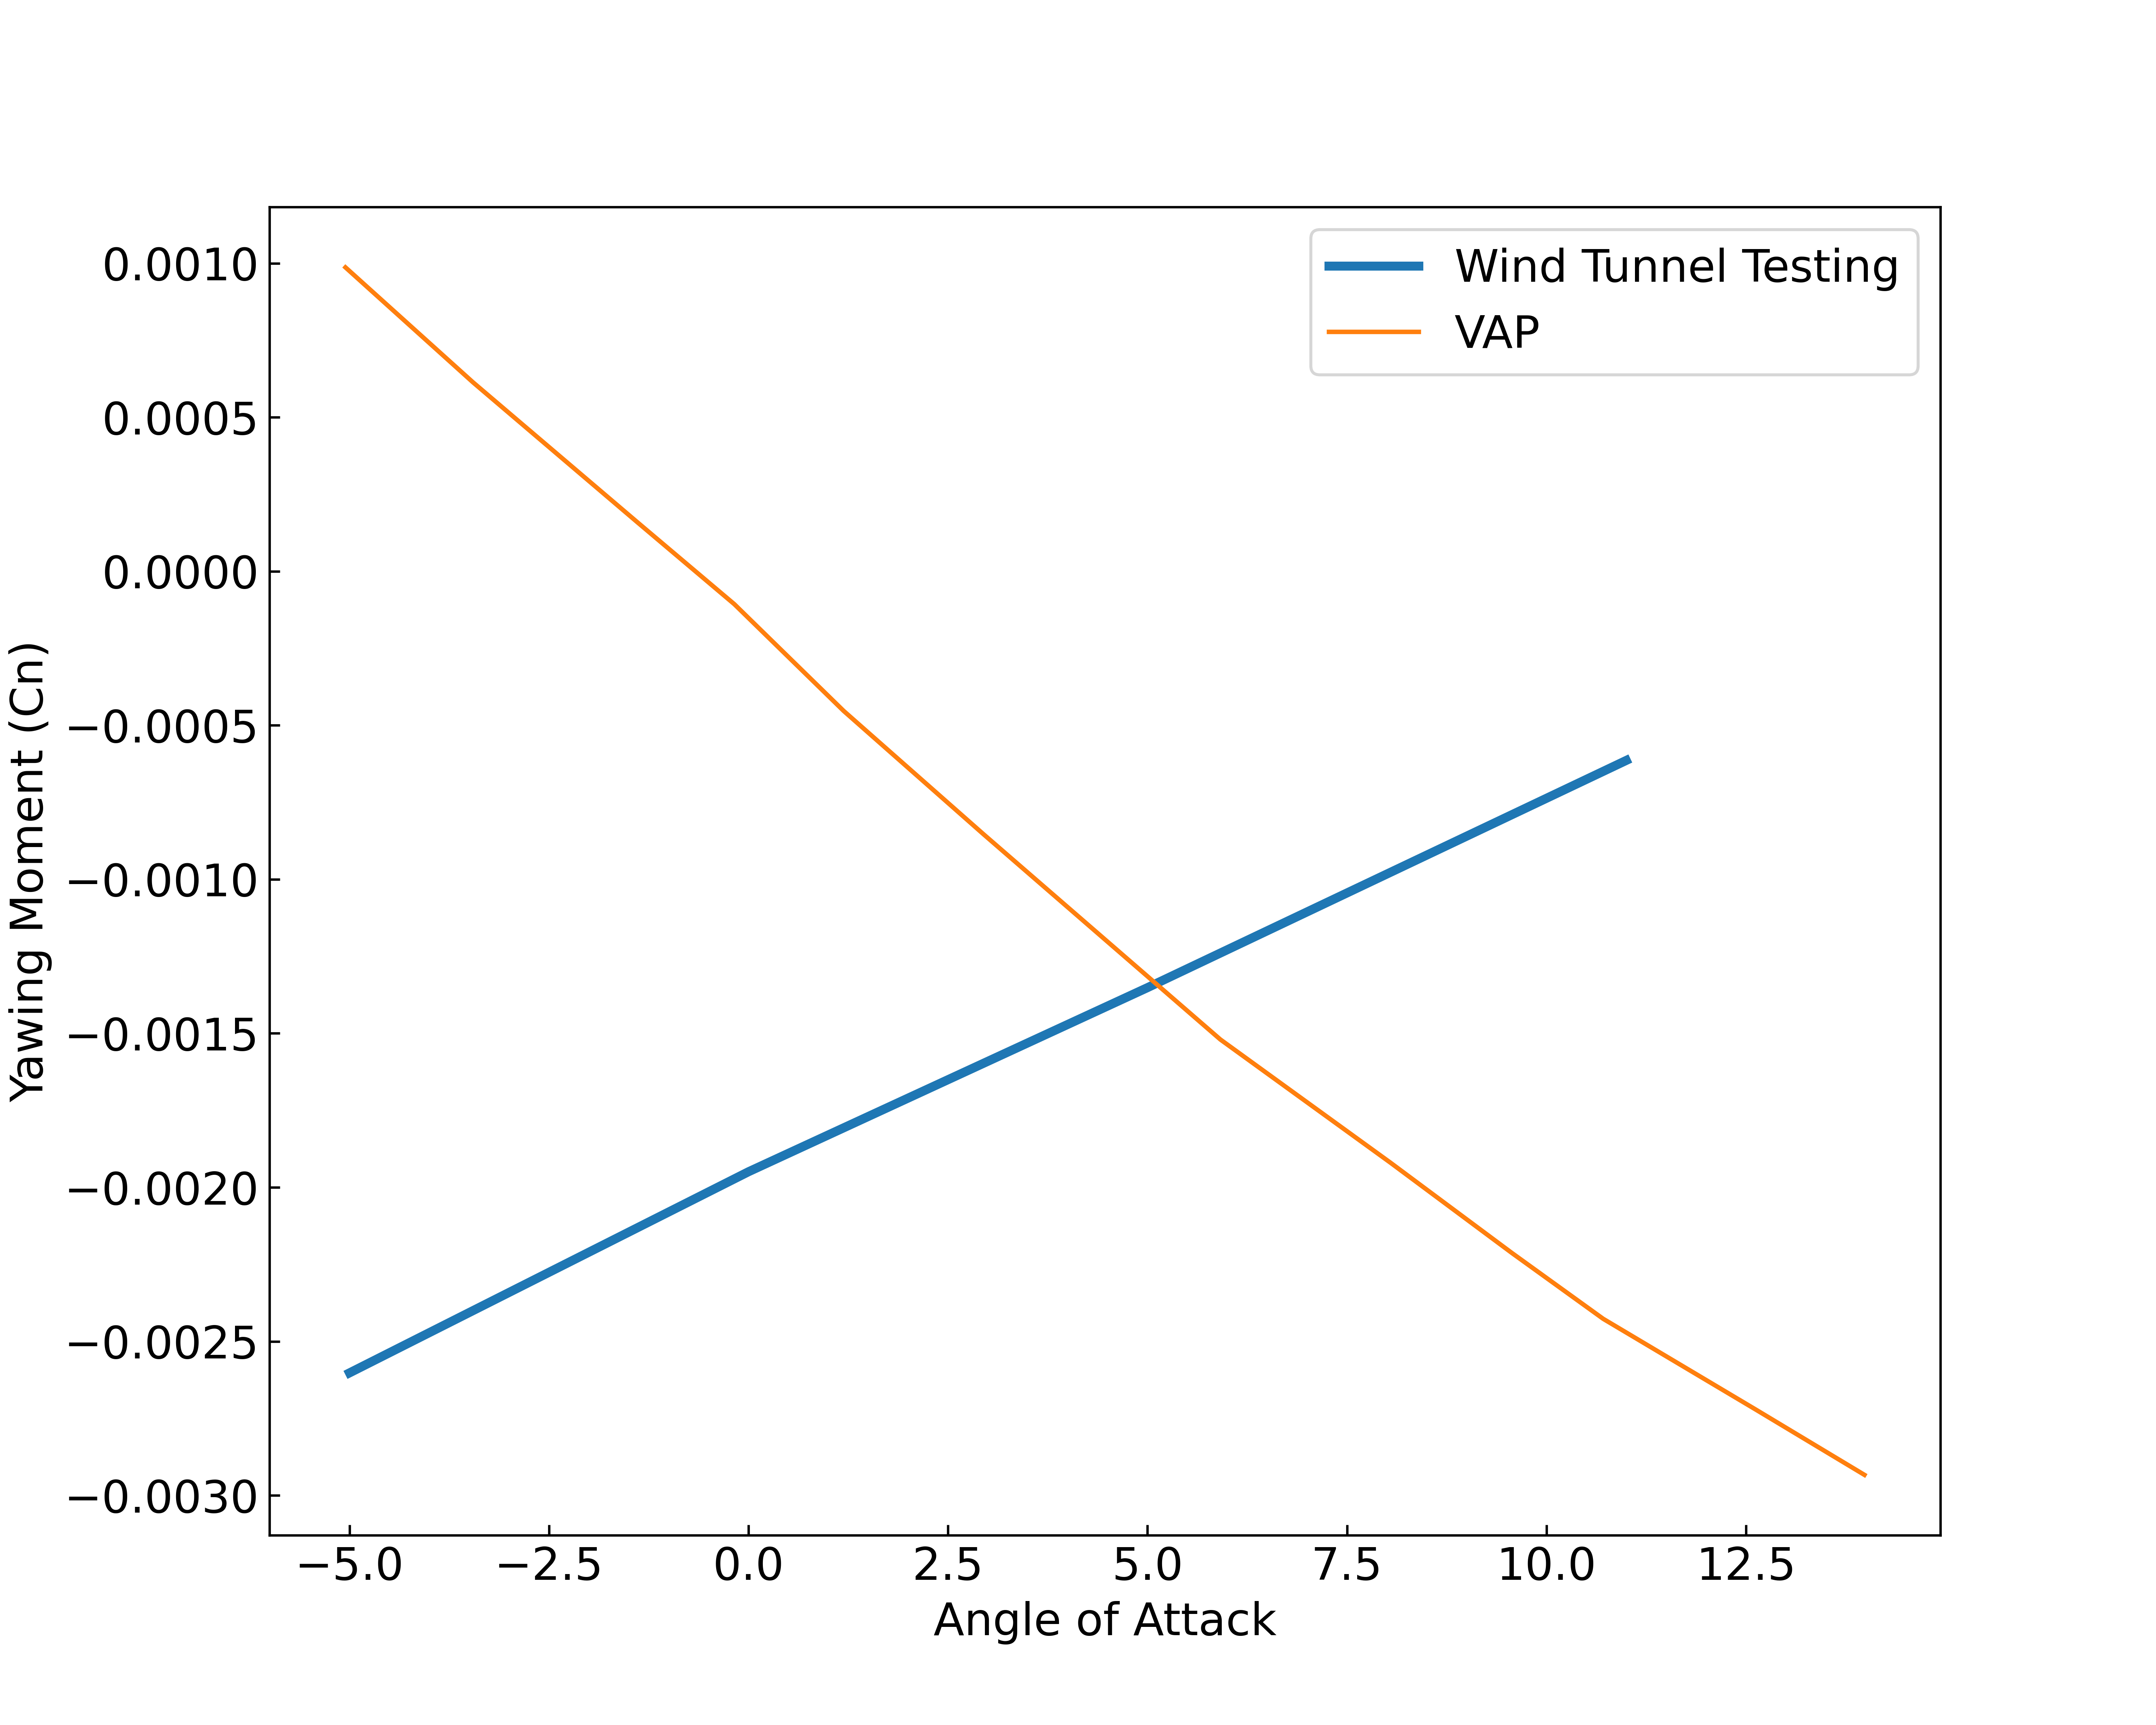
\includegraphics[width=\textwidth]{05_Results/VAP/noProp/Cn/20ms_6000RPM_Cn.png}
        \caption{Yawing Moment Coefficient at 20m/s airspeed for no propeller configuration}
        \label{fig:VAP_noProp_Cn_20ms_6000}
    \end{subfigure}
    \begin{subfigure}[b]{0.467\textwidth}
        \centering
        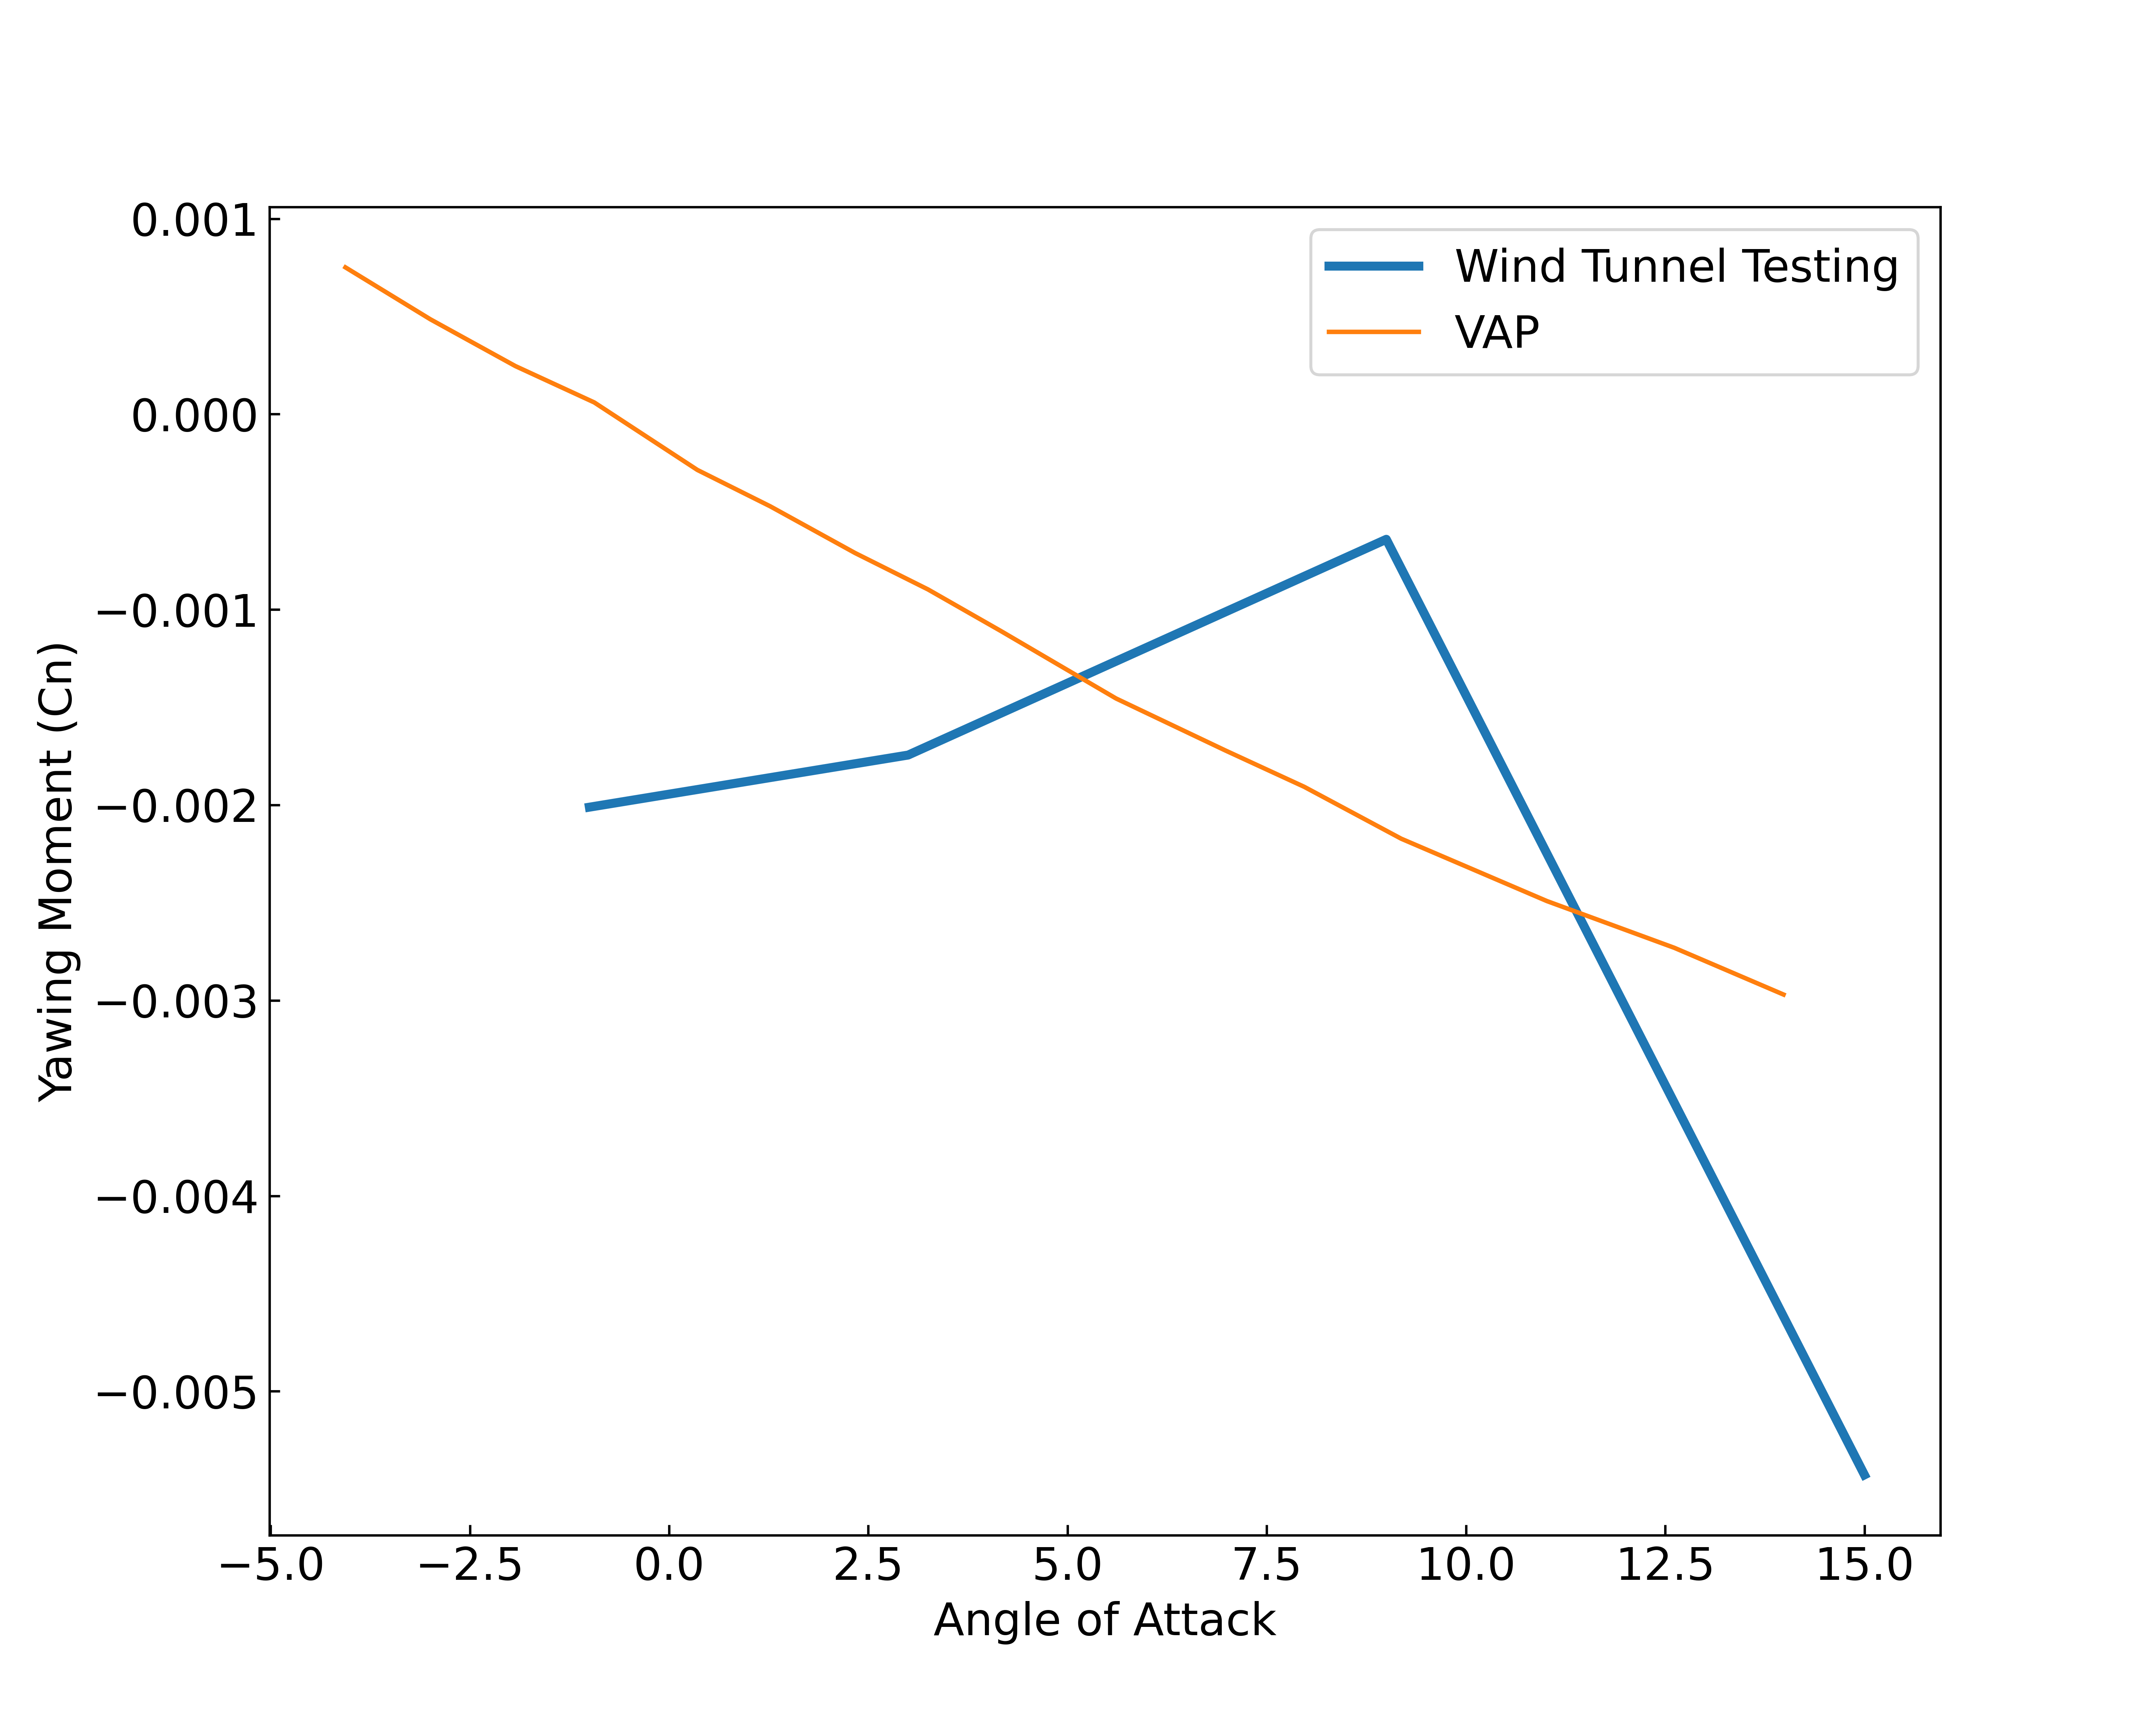
\includegraphics[width=\textwidth]{05_Results/VAP/noProp/Cn/20ms_11000RPM_Cn.png}
        \caption{Yawing Moment Coefficient at 20m/s airspeed for no propeller configuration}
        \label{fig:VAP_noProp_Cn_20ms_11000}
    \end{subfigure}
\end{figure}



\subsubsection{Tractor Configuration}

The tractor configuration introduced a propeller in the VAP 3.5 simulations. As VAP 3.5 is still currently testing these calculations. For propeller calculations, the side forces and moment calculation methods are still in testing. The simulation for the tractor configuration was run until the propeller wake passed over the tail so that the wake interactions had been fully developed to assess the stability coefficients. Figure \ref{fig:tractorwake} shows a partially developed wake.

\begin{figure}[H]
\centering
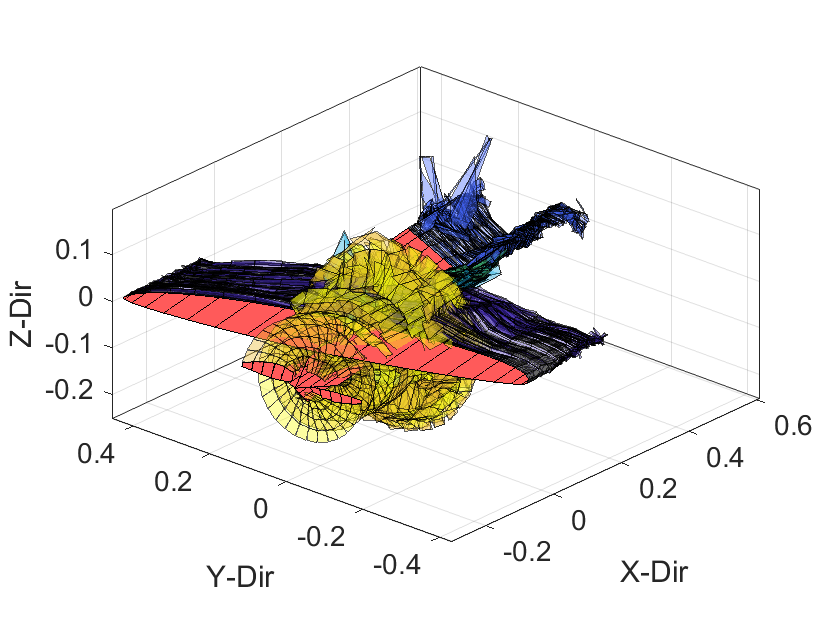
\includegraphics[width=0.5\linewidth]{05_Results/Figs/VAP/model.png}
\caption{VAP 3.5 simulation of tractor configuration showing propeller-wing wake interference}
\label{fig:tractorwake}
\end{figure}

The rolling moment of the VAP 3.5 software showed substantial discrepancies in magnitude and trend for Figures \ref{fig:VAP_Cl_10ms_6000} to \ref{fig:VAP_Cl_20ms_6000}. Figure \ref{fig:VAP_Cl_20ms_11000} begins to show similar trends to the wind tunnel tested results. However, the discrepancy is still too large to show an agreement. This is likely caused by the force and moments from the propeller and has not been tested with accurate results. The discrepancy can also be attributed to the geometry of the VAP 3.5 model, as it simplifies the actual \acrshort{MAV} geometry.


\begin{figure}[H]
    \centering
    \begin{subfigure}[b]{0.467\textwidth}
        \centering
        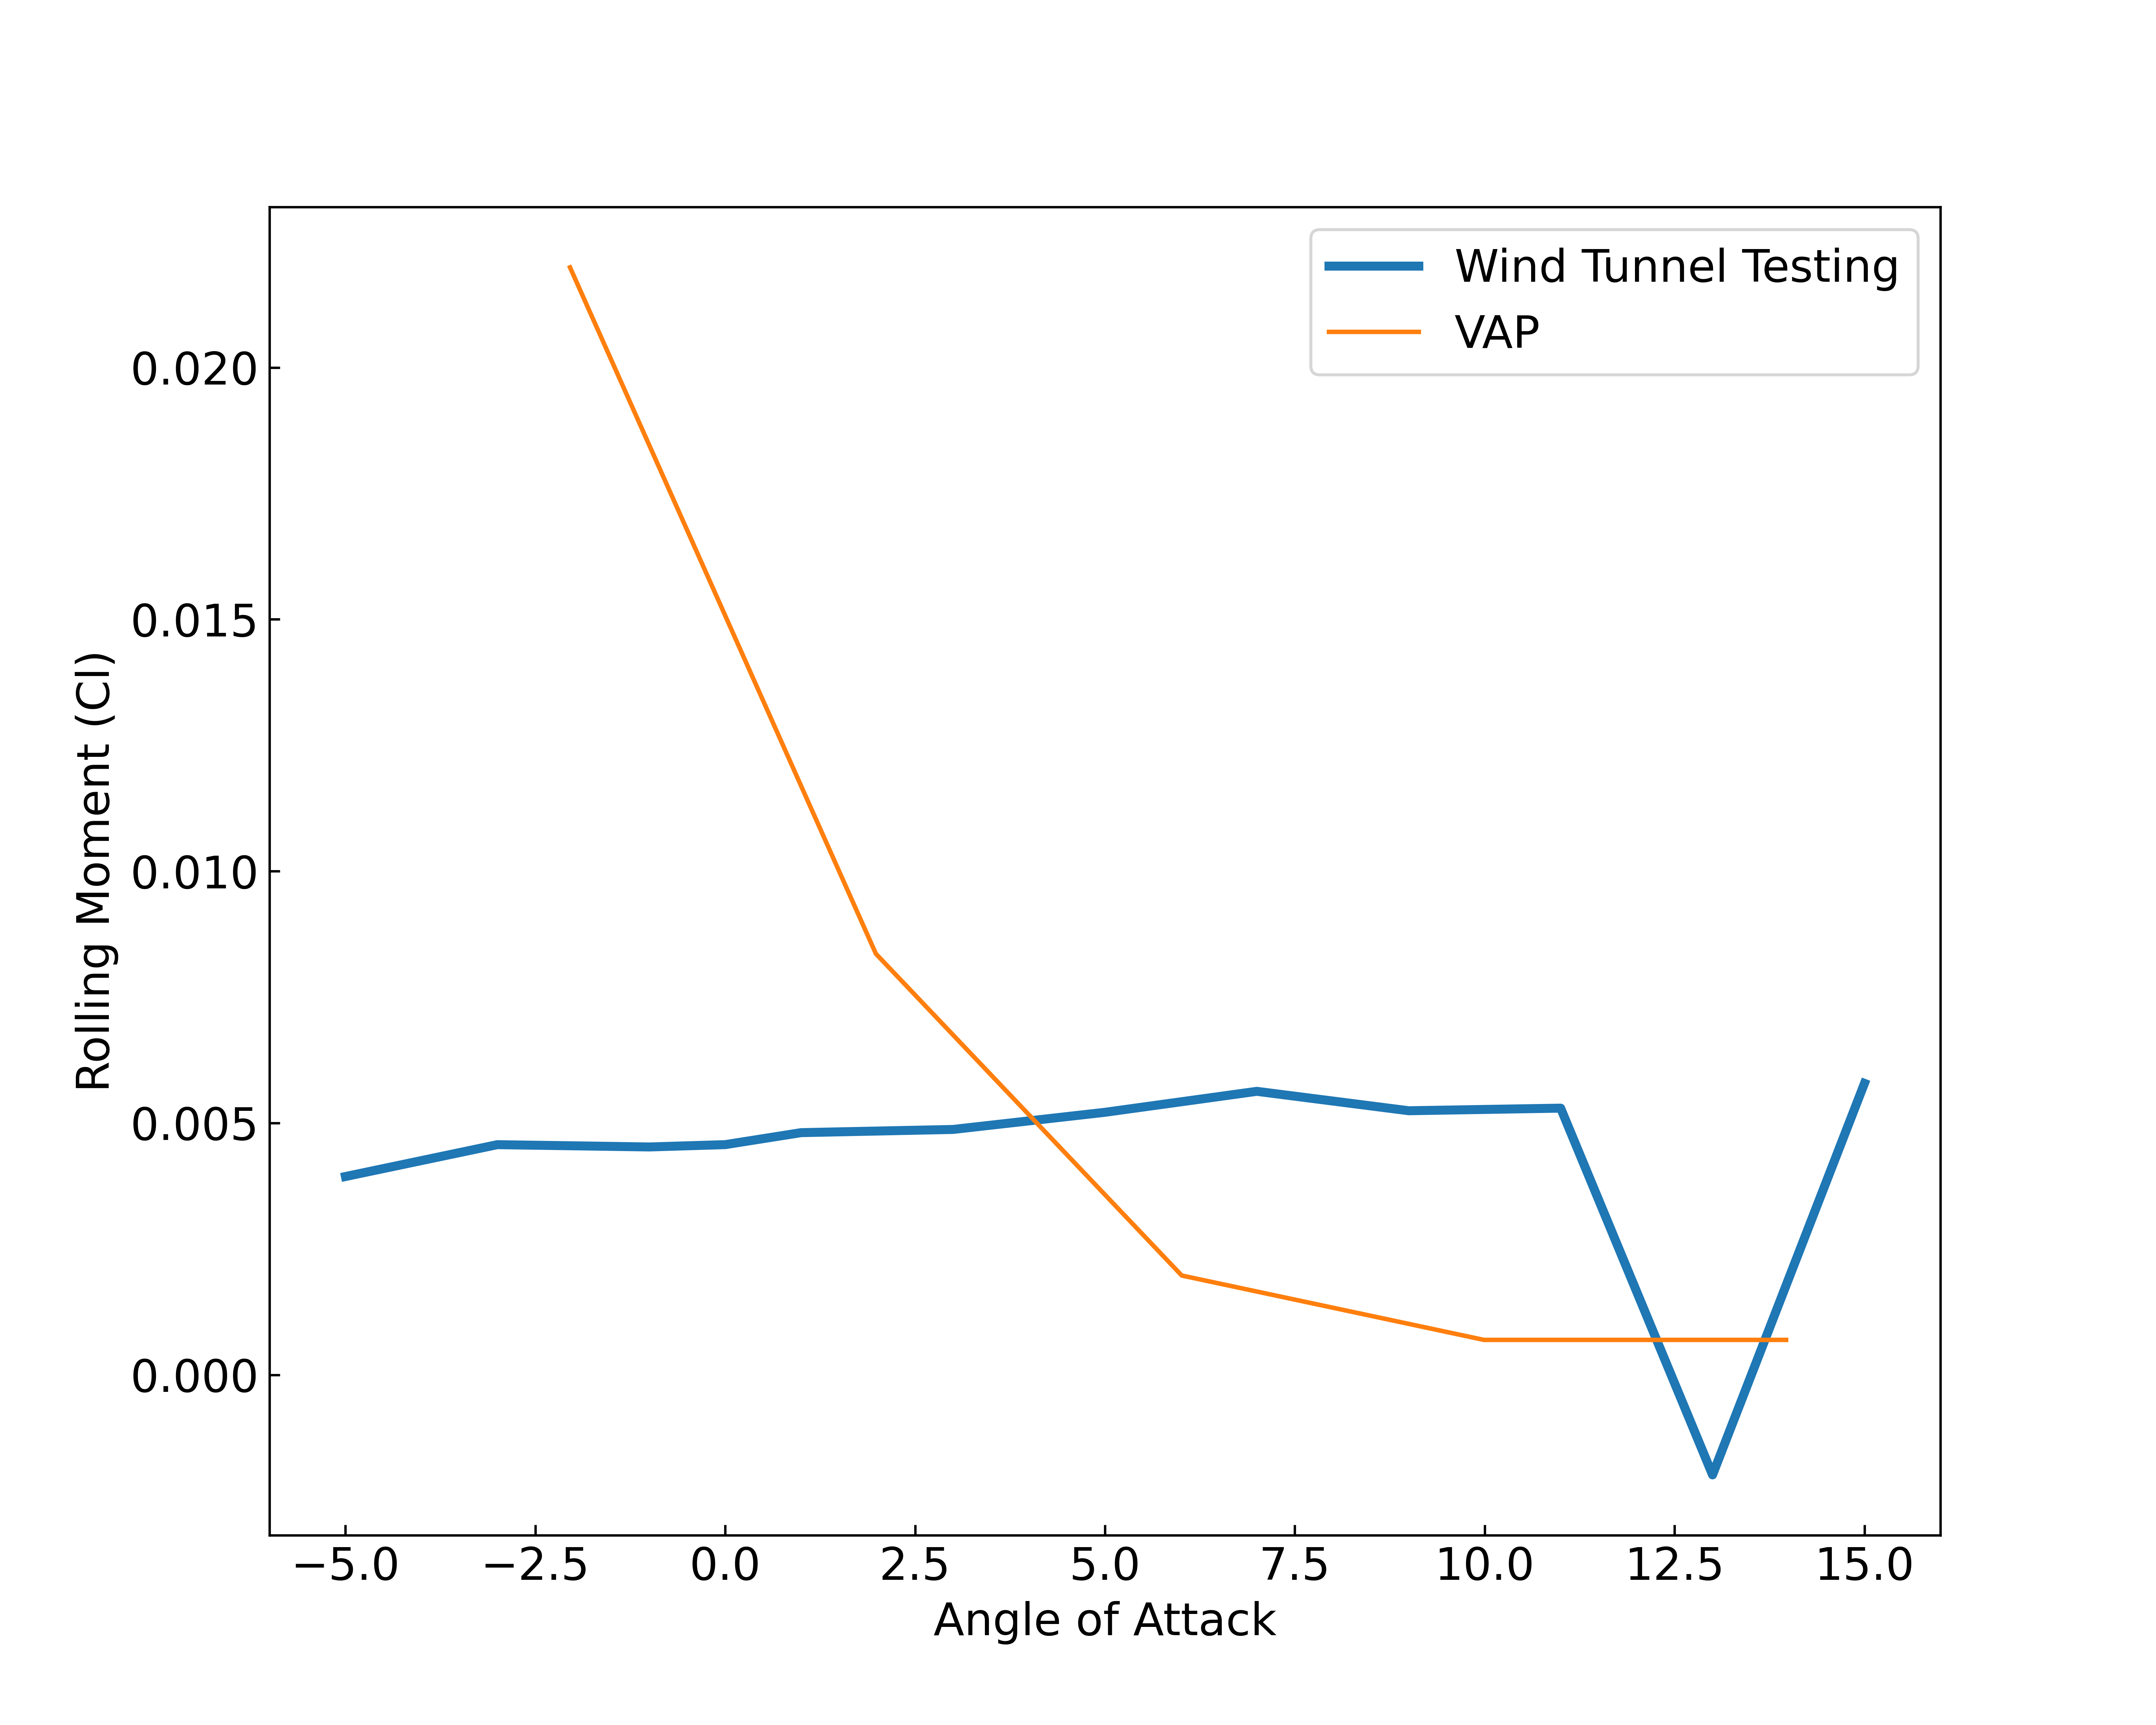
\includegraphics[width=\textwidth]{05_Results/VAP/tractor/Cl/10ms_6000RPM_Cl.png}
        \caption{Rolling Moment Coefficient at 10m/s airspeed and 6000RPM motor speed}
        \label{fig:VAP_Cl_10ms_6000}
    \end{subfigure}
    \begin{subfigure}[b]{0.467\textwidth}
        \centering
        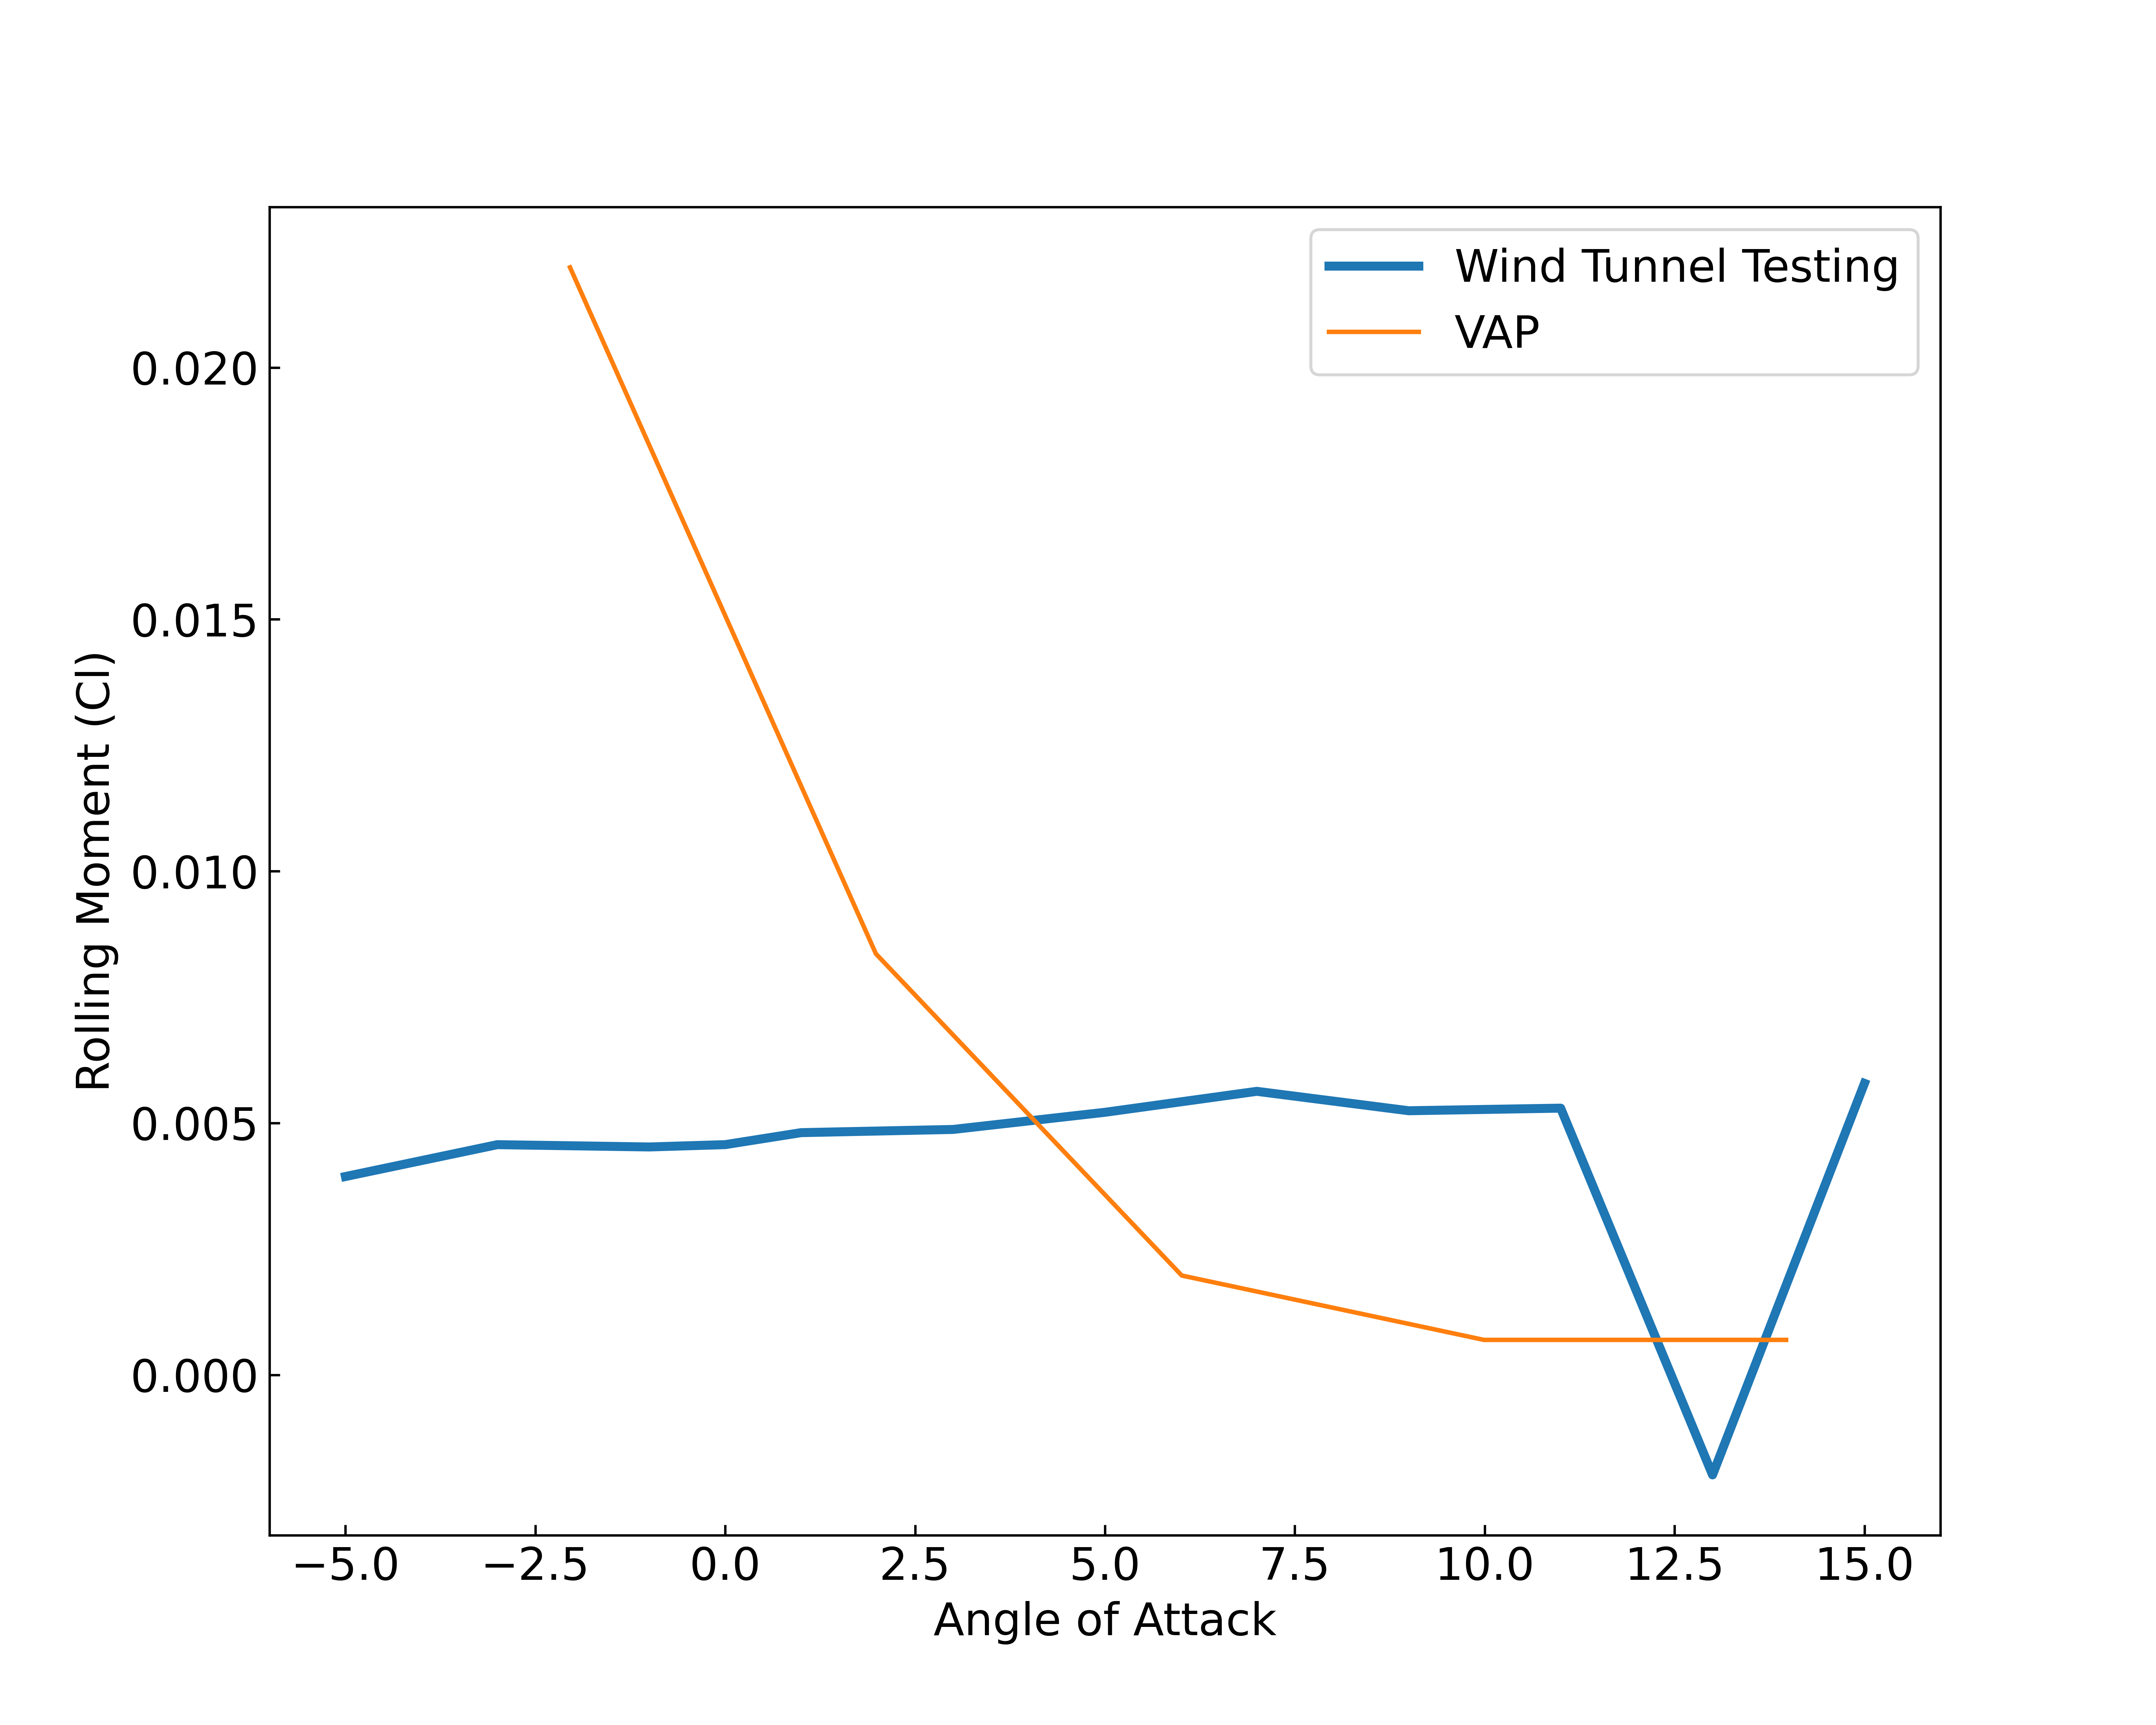
\includegraphics[width=\textwidth]{05_Results/VAP/tractor/Cl/10ms_6000RPM_Cl.png}
        \caption{Rolling Moment Coefficient at 10m/s airspeed and 11000RPM motor speed}
        \label{fig:Missing2}
    \end{subfigure}
    \begin{subfigure}[b]{0.467\textwidth}
        \centering
        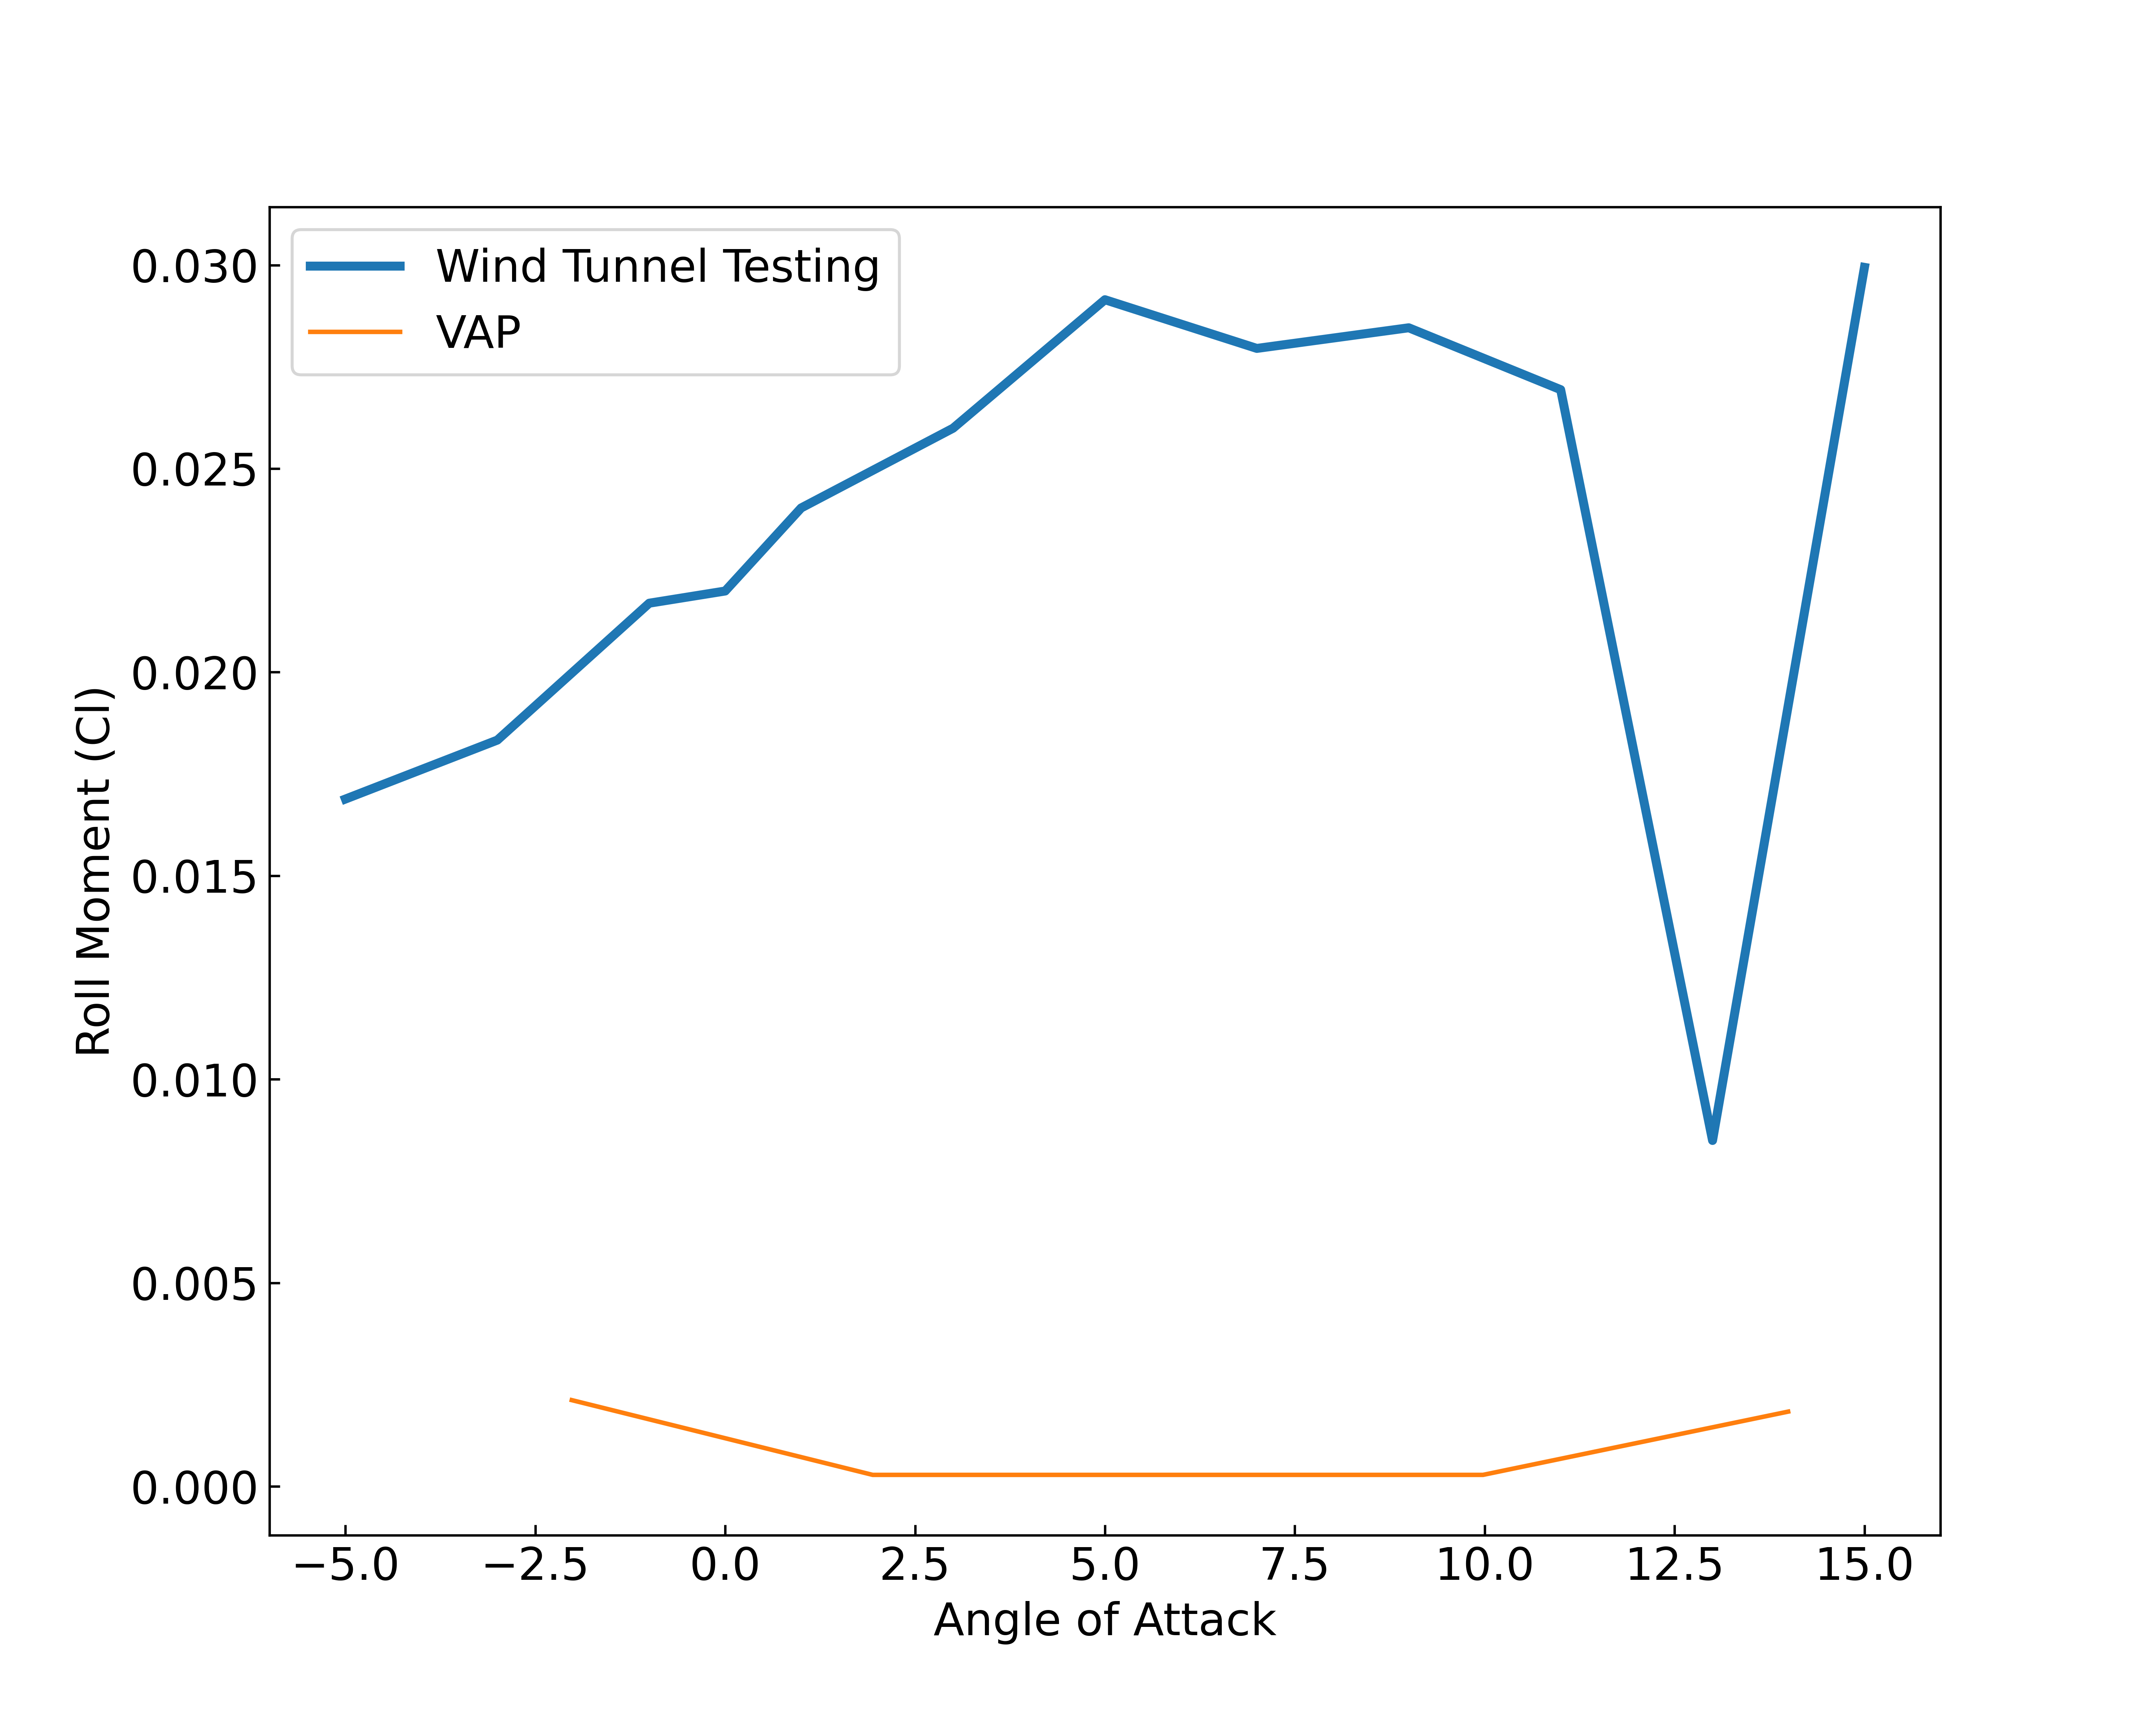
\includegraphics[width=\textwidth]{05_Results/VAP/tractor/Cl/20ms_6000RPM_Cl.png}
        \caption{Rolling Moment Coefficient at 20m/s airspeed and 6000RPM motor speed}
        \label{fig:VAP_Cl_20ms_6000}
    \end{subfigure}
    \begin{subfigure}[b]{0.467\textwidth}
        \centering
        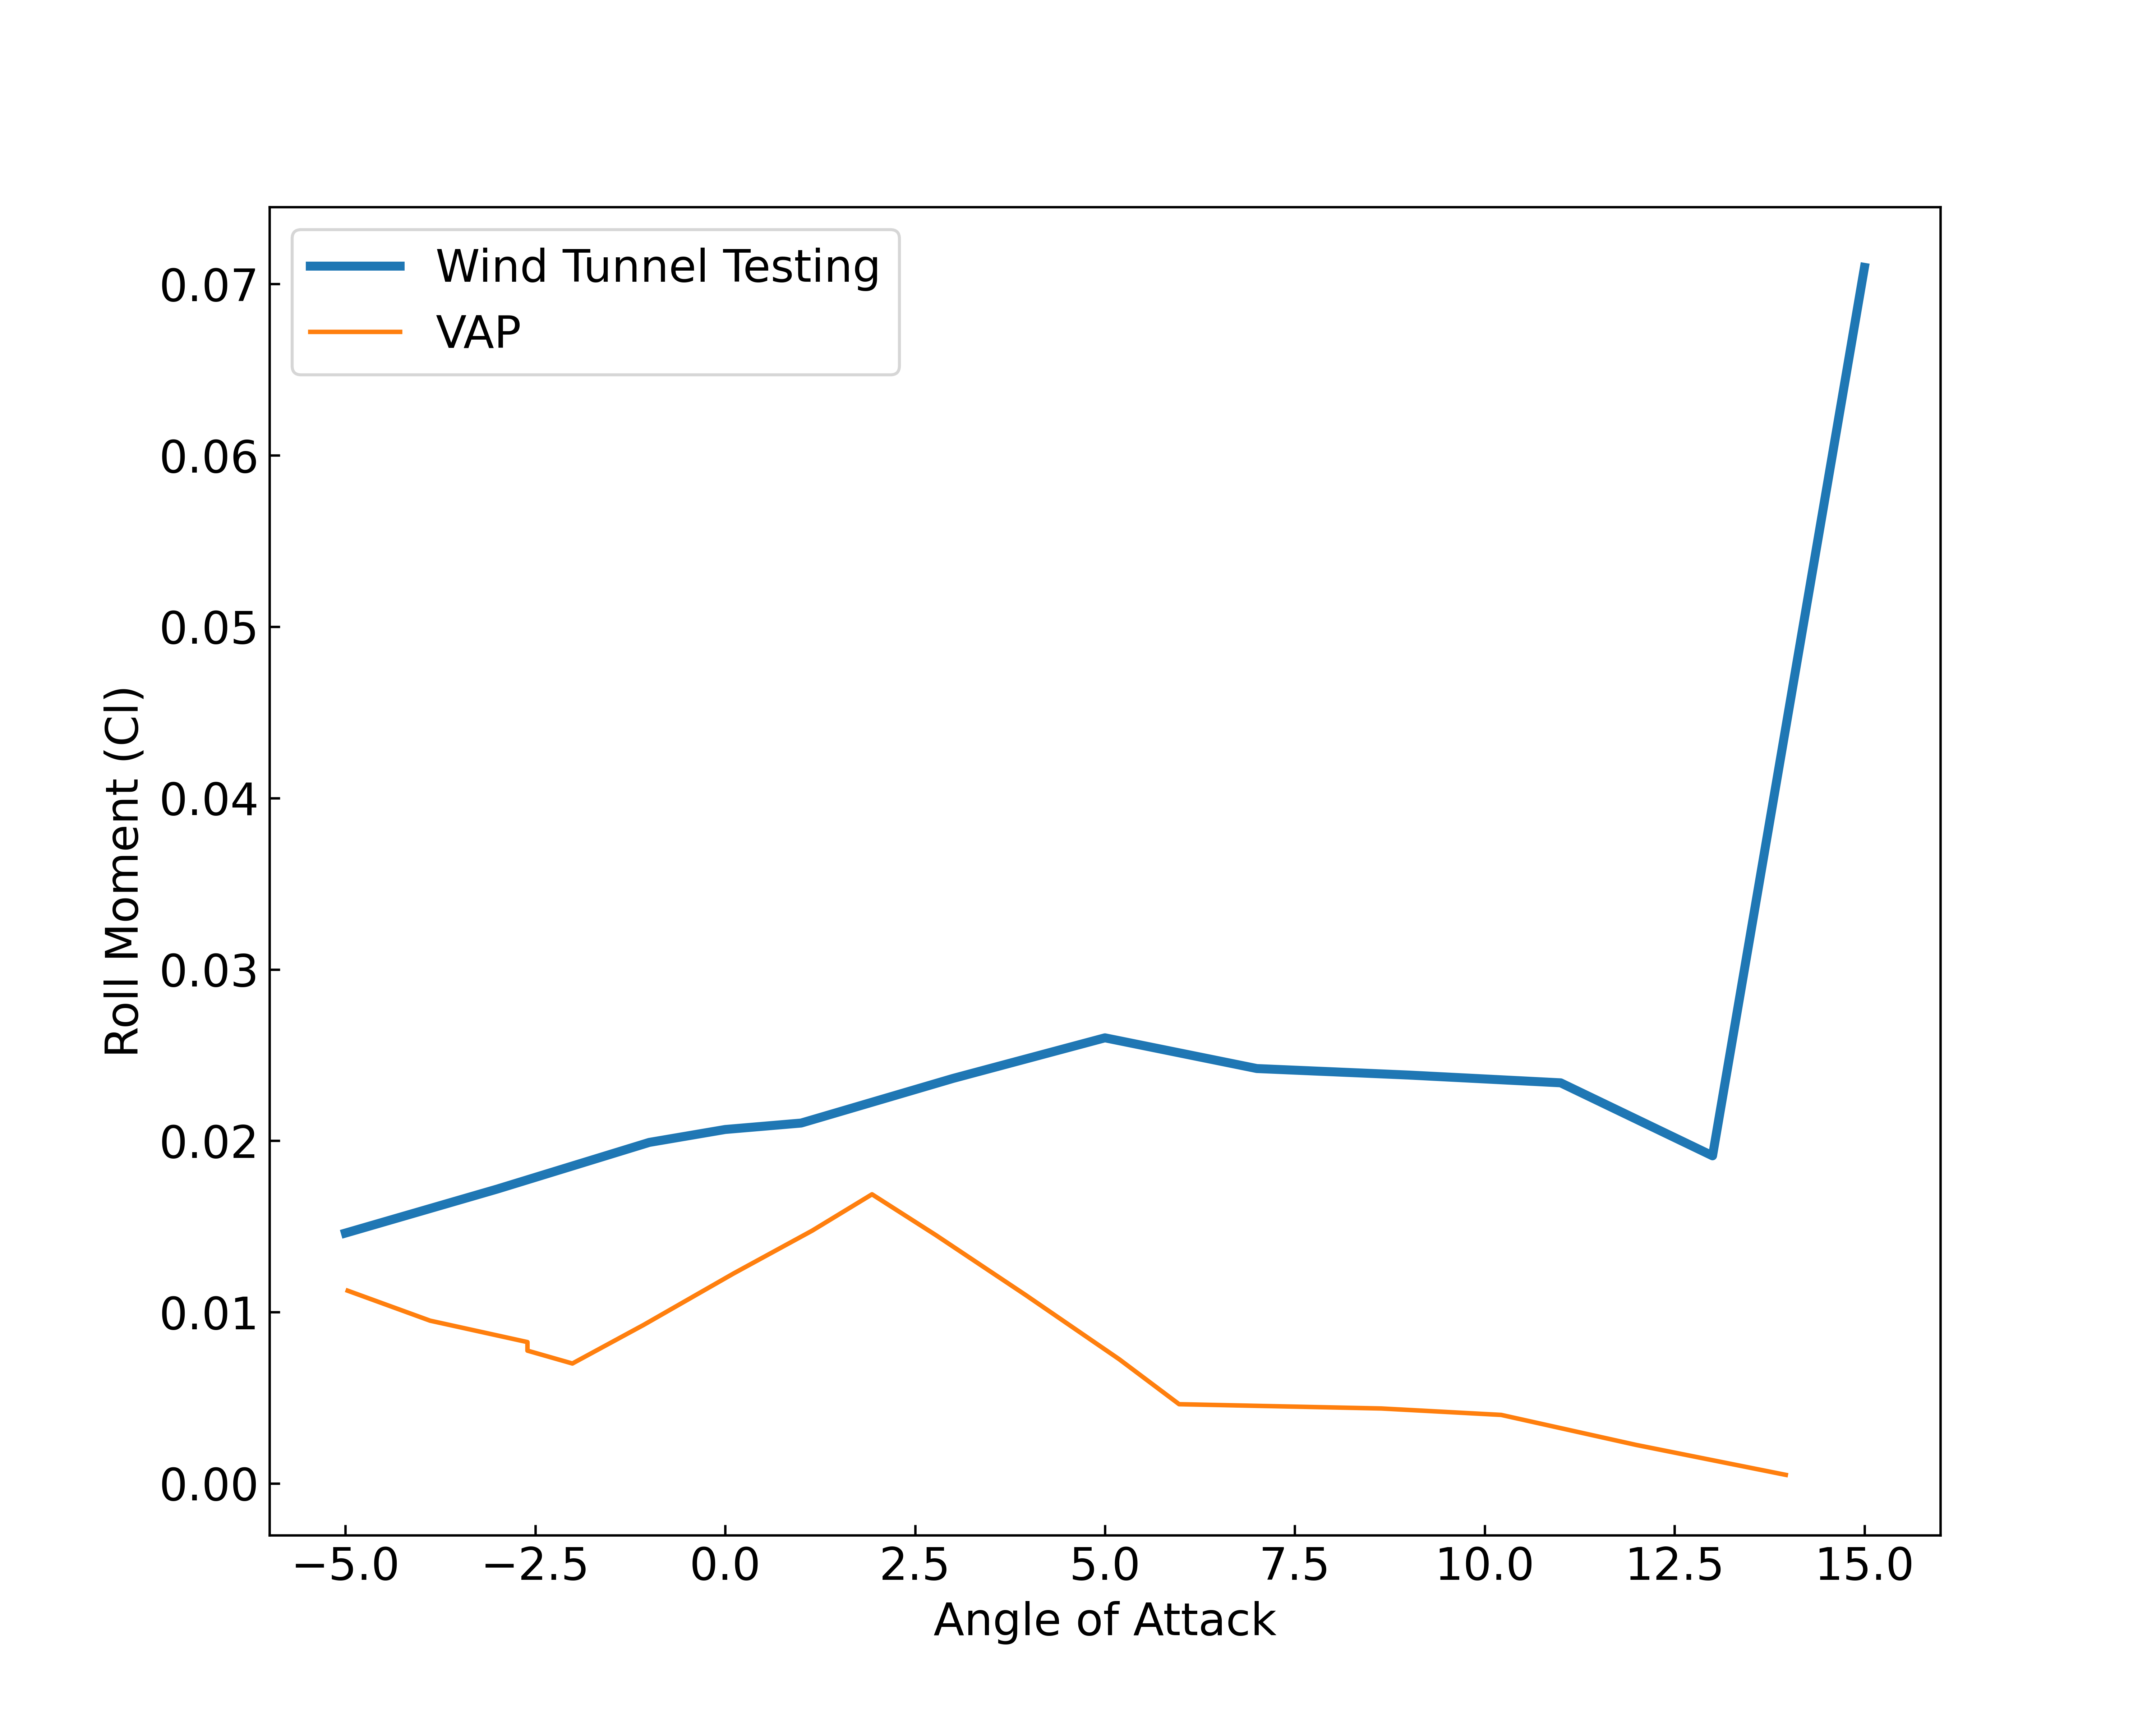
\includegraphics[width=\textwidth]{05_Results/VAP/tractor/Cl/20ms_11000RPM_Cl.png}
        \caption{Rolling Moment Coefficient at 20m/s airspeed and 11000RPM motor speed}
        \label{fig:VAP_Cl_20ms_11000}
    \end{subfigure}
\end{figure}

While the pitching moment showed the same general trend for the no-propeller analysis, the addition of the propeller significantly reduced the accuracy of the pitching moment coefficient. The addition of random increases in pitching moment such as that seen at 7$^\circ$ \acrshort{AoA} in Figure \ref{fig:VAP_Cl_10ms_6000} are unexpected and shows that there still needs to be a further improvement on the method which is being used to calculate the forces and moments created by the aircraft, along with how these translate to the main \acrshort{MAV} model. 

\begin{figure}[H]
    \centering
    \begin{subfigure}[b]{0.467\textwidth}
        \centering
        \includegraphics[width=\textwidth]{05_Results/VAP/tractor/Cm/10ms_6000RPM_Cm.png}
        \caption{Pitching Moment Coefficient at 10m/s airspeed and 6000RPM motor speed}
        \label{fig:VAP_Cm_10ms_6000}
    \end{subfigure}
    \begin{subfigure}[b]{0.467\textwidth}
        \centering
        \includegraphics[width=\textwidth]{05_Results/VAP/tractor/Cm/10ms_11000RPM_Cm.png}
        \caption{Pitching Moment Coefficient at 10m/s airspeed and 11000RPM motor speed}
        \label{fig:VAP_Cm_10ms_11000}
    \end{subfigure}
    \begin{subfigure}[b]{0.467\textwidth}
        \centering
        \includegraphics[width=\textwidth]{05_Results/VAP/tractor/Cm/20ms_6000RPM_Cm.png}
        \caption{Pitching Moment Coefficient at 20m/s airspeed and 6000RPM motor speed}
        \label{fig:VAP_Cm_20ms_6000}
    \end{subfigure}
    \begin{subfigure}[b]{0.467\textwidth}
        \centering
        \includegraphics[width=\textwidth]{05_Results/VAP/tractor/Cm/20ms_11000RPM_Cm.png}
        \caption{Pitching Moment Coefficient at 20m/s airspeed and 11000RPM motor speed}
        \label{fig:VAP_Cm_20ms_11000}
    \end{subfigure}
\end{figure}


Figures \ref{fig:VAP_tractor_10ms_11000} to \ref{fig:VAP_Cn_20ms_11000} show the yaw moment comparison between the VAP 3.5 and wind tunnel results. The yawing moment is primarily influenced by the roll of the \acrshort{MAV}, and wind tunnel testing showed a sharp drop in some instances due to the right wing stalling before the left. There is a significant gradient change in Figure \ref{fig:VAP_tractor_10ms_11000} as the \acrshort{AoA} transitions from negative to positive. From 6$^\circ$ \acrshort{AoA}, the gradient of the yawing moment is significantly closer to what is expected. However, there is no general agreement between the VAP 3.5 and wind tunnel results in all cases analysed. The higher 20m$s^{-1}$ results shown in Figure \ref{fig:VAP_Cn_20ms_6000} and \ref{fig:VAP_Cn_20ms_11000} in particular show a trend which is opposite to what is expected from wind tunnel testing and again is likely due to the same force and moment methods still being under development and testing. 

\begin{figure}[H]
    \centering
    \begin{subfigure}[b]{0.467\textwidth}
        \centering
        \includegraphics[width=\textwidth]{05_Results/VAP/tractor/Cn/10ms_11000RPM_Cn.png}
        \caption{Yawing Moment Coefficient at 10m/s airspeed and 11000RPM motor speed}
        \label{fig:VAP_tractor_10ms_11000}
    \end{subfigure}
    \begin{subfigure}[b]{0.467\textwidth}
        \centering
        \includegraphics[width=\textwidth]{05_Results/VAP/tractor/Cn/20ms_6000RPM_Cn.png}
        \caption{Yawing Moment Coefficient at 20m/s airspeed and 6000RPM motor speed}
        \label{fig:VAP_Cn_20ms_6000}
    \end{subfigure}
    \begin{subfigure}[b]{0.467\textwidth}
        \centering
        \includegraphics[width=\textwidth]{05_Results/VAP/tractor/Cn/20ms_11000RPM_Cn.png}
        \caption{Yawing Moment Coefficient at 20m/s airspeed and 11000RPM motor speed}
        \label{fig:VAP_Cn_20ms_11000}
    \end{subfigure}
\end{figure}


\subsubsection{Pusher Configuration}

A fully developed wake flow for the pusher configuration is shown in Figures \ref{fig:TractorCofigurationWake} and \ref{fig:TractorCofigurationWake2}. The simulation was run until the wake from the wing had passed over the propeller at the rear of the \acrshort{MAV} model.

\begin{figure}[H]
    \centering
    \begin{subfigure}[b]{0.467\textwidth}
      \centering
        \includegraphics[width=\textwidth]{05_Results/Figs/VAP/fullyDevelopedWake.png}
        \caption{Side view of the fully developed wake for the pusher configuration in VAP 3.5}
        \label{fig:TractorCofigurationWake}
         \end{subfigure}
          \begin{subfigure}[b]{0.467\textwidth}
      \centering
        \includegraphics[width=\textwidth]{05_Results/Figs/VAP/fullyDevelopedWake2.png}
        \caption{Top view of the fully developed wake for the pusher configuration in VAP 3.5}
        \label{fig:TractorCofigurationWake2}
         \end{subfigure}
\end{figure}


The rolling moment of the VAP 3.5 software showed substantial discrepancies in magnitude and trend for Figures \ref{fig:VAP_pusher_Cl_10ms_6000} to \ref{fig:VAP_pusher_Cl_20ms_11000}. As the pusher configuration also includes a propeller, the discrepancy is likely caused by the force and moments from the propeller, as previously explained. Figure \ref{fig:VAP_psuher_Cl_20ms_6000} also implies that the motor torque effect has not been included in calculations to determine the stability coefficients as the rolling moment is very close to 0, which is unexpected due to the propeller torque effect, which should be generated as the wings experience an upwash on one side and a downwash on the other side of the propeller wake.

\begin{figure}[H]
    \centering
    \begin{subfigure}[b]{0.467\textwidth}
        \centering
        \includegraphics[width=0.8\textwidth]{05_Results/VAP/pusher/Cl/10ms_6000RPM_Cl.png}
        \caption{Rolling Moment Coefficient at 10m/s airspeed and 6000RPM motor speed}
        \label{fig:VAP_pusher_Cl_10ms_6000}
    \end{subfigure}
    \begin{subfigure}[b]{0.467\textwidth}
        \centering
        \includegraphics[width=0.8\textwidth]{05_Results/VAP/pusher/Cl/10ms_11000RPM_Cl.png}
        \caption{Rolling Moment Coefficient at 10m/s airspeed and 11000RPM motor speed}
        \label{fig:VAP_pusher_Cl_10ms_11000}
    \end{subfigure}
    \begin{subfigure}[b]{0.467\textwidth}
        \centering
        \includegraphics[width=0.8\textwidth]{05_Results/VAP/pusher/Cl/20ms_6000RPM_Cl.png}
        \caption{Rolling Moment Coefficient at 20m/s airspeed and 6000RPM motor speed}
        \label{fig:VAP_psuher_Cl_20ms_6000}
    \end{subfigure}
    \begin{subfigure}[b]{0.467\textwidth}
        \centering
        \includegraphics[width=0.8\textwidth]{05_Results/VAP/pusher/Cl/20ms_11000RPM_Cl.png}
        \caption{Rolling Moment Coefficient at 20m/s airspeed and 11000RPM motor speed}
        \label{fig:VAP_pusher_Cl_20ms_11000}
    \end{subfigure}
\end{figure}

Figures \ref{fig:VAP_pusher_Cm_10ms_6000} to \ref{fig:VAP_pusher_Cm_20ms_11000} show that the pitching moment was estimated to be larger in magnitude for the VAP 3.5 simulations. The same curve shown in all conditions analysed is not seen in the VAP 3.5 estimations, which are more linear than expected. These discrepancies are likely due to the missing propeller effects that need to be accounted for in a propelled model. 


\begin{figure}[H]
    \centering
    \begin{subfigure}[b]{0.467\textwidth}
        \centering
        \includegraphics[width=\textwidth]{05_Results/VAP/pusher/Cm/10ms_6000RPM_Cm.png}
        \caption{Pitching Moment Coefficient at 10m/s airspeed and 6000RPM motor speed}
        \label{fig:VAP_pusher_Cm_10ms_6000}
    \end{subfigure}
    \begin{subfigure}[b]{0.467\textwidth}
        \centering
        \includegraphics[width=\textwidth]{05_Results/VAP/pusher/Cm/10ms_11000RPM_Cm.png}
        \caption{Pitching Moment Coefficient at 10m/s airspeed and 11000RPM motor speed}
        \label{fig:VAP_pusher_Cm_10ms_11000}
    \end{subfigure}
    \begin{subfigure}[b]{0.467\textwidth}
        \centering
        \includegraphics[width=\textwidth]{05_Results/VAP/pusher/Cm/20ms_6000RPM_Cm.png}
        \caption{Pitching Moment Coefficient at 20m/s airspeed and 6000RPM motor speed}
        \label{fig:VAP_pusher_Cm_20ms_6000}
    \end{subfigure}
    \begin{subfigure}[b]{0.467\textwidth}
        \centering
        \includegraphics[width=\textwidth]{05_Results/VAP/pusher/Cm/20ms_11000RPM_Cm.png}
        \caption{Pitching Moment Coefficient at 20m/s airspeed and 11000RPM motor speed}
        \label{fig:VAP_pusher_Cm_20ms_11000}
    \end{subfigure}
\end{figure}


 Figures \ref{fig:VAP_pusher_Cn_10ms_6000} to \ref{fig:VAP_pusher_Cn_20ms_11000}, similarly to the tractor configuration, show a trend that is opposite to what is expected from wind tunnel testing and again is likely due to the same force and moment methods still being under development and testing. 
 
\begin{figure}[H]
    \centering
    \begin{subfigure}[b]{0.467\textwidth}
        \centering
        \includegraphics[width=\textwidth]{05_Results/VAP/pusher/Cn/10ms_6000RPM_Cn.png}
        \caption{Yawing Moment Coefficient at 10m/s airspeed and 6000RPM motor speed}
        \label{fig:VAP_pusher_Cn_10ms_6000}
    \end{subfigure}
    \begin{subfigure}[b]{0.467\textwidth}
        \centering
        \includegraphics[width=\textwidth]{05_Results/VAP/pusher/Cn/10ms_11000RPM_Cn.png}
        \caption{Yawing Moment Coefficient at 10m/s airspeed and 11000RPM motor speed}
        \label{fig:VAP_pusherr_Cn_10ms_11000}
    \end{subfigure}
    \begin{subfigure}[b]{0.467\textwidth}
        \centering
        \includegraphics[width=\textwidth]{05_Results/VAP/pusher/Cn/20ms_6000RPM_Cn.png}
        \caption{Yawing Moment Coefficient at 20m/s airspeed and 6000RPM motor speed}
        \label{fig:VAP_pusher_Cn_20ms_6000}
    \end{subfigure}
    \begin{subfigure}[b]{0.467\textwidth}
        \centering
        \includegraphics[width=\textwidth]{05_Results/VAP/pusher/Cn/20ms_11000RPM_Cn.png}
        \caption{Yawing Moment Coefficient at 20m/s airspeed and 11000RPM motor speed}
        \label{fig:VAP_pusher_Cn_20ms_11000}
    \end{subfigure}
\end{figure}


